\documentclass[a4paper,fleqn]{cas-dc}
%\documentclass[a4paper,fleqn,longmktitle]{cas-dc}
\def\input@path{/home/isaac/geomagnetic_local_effects_p1/cas-dc.cls}

% If the frontmatter runs over more than one page
% use the longmktitle option.



\usepackage[numbers]{natbib}
%\usepackage[authoryear]{natbib}
\usepackage{comment}

%\usepackage{lastpage}
%\usepackage{blindtext}
%\usepackage[authoryear,longnamesfirst]{natbib}

%%%Author macros
\def\tsc#1{\csdef{#1}{\textsc{\lowercase{#1}}\xspace}}
\tsc{WGM}
\tsc{QE}
%%%
% Uncomment and use as if needed
%\newtheorem{theorem}{Theorem}
%\newtheorem{lemma}[theorem]{Lemma}
%\newdefinition{rmk}{Remark}
%\newproof{pf}{Proof}
%\newproof{pot}{Proof of Theorem \ref{thm}}
\begin{document}
\let\WriteBookmarks\relax
\def\floatpagepagefraction{1}
\def\textpagefraction{.001}

% Short title
\shorttitle{Geomagnetic local response associated with geomagnetic storms}    

% Short author
\shortauthors{Castellanos-Velazco, C. I. et al.}  

% Main title of the paper
\title [mode = title]{Low latitude geomagnetic response associated with intense geomagnetic storms: regional space weather in Mexico}  

% Title footnote mark
% eg: \tnotemark[1]
%\tnotemark[<tnote number>] 

% Title footnote 1.
% eg: \tnotetext[1]{Title footnote text}
%\tnotetext[<tnote number>]{<tnote text>} 

%First author

\author[1]{Castellanos-Velazco, C. I.} [type=editor, orcid=0000-0001-8818-5318]

% Footnote of the first author
%\fnmark[<footnote mark no>]

% Email id of the first author
\ead{ccastellanos@igeofisica.unam.mx}

% URL of the first author
%\ead[url]{<URL>}

\credit{Methodology, Conceptualization, Data analysis, Software, Writing - Original Draft}

%Second author
\author[2]{Corona-Romero, P.}[orcid=0000-0002-2573-2967]
\credit{Conceptualization, Methodology, Software, Writing - Review \& Editing}
\ead{p.coronaromero@igeofisica.unam.mx}

\author[2]{ González-Esparza, J. A.}[orcid=0000-0003-4774-1829]
\credit{Data revision, Review \& Editing}
\ead{americo@igeofisica.unam.mx}

\author[3]{ Caccavari-Garza, A. L.}[]
\credit{Regional magnetic data, Review \& Editing}
\author[2]{ Sergeeva, M. A.}[]
\credit{Local ionospheric data, Review \& Editing}
% Corresponding author indication
\cormark[2]

% Footnote of the second author
%\fnmark[2]

% Email id of the second author


% URL of the second author
%\ead[url]{}

% Credit authorship


% Address/affiliation
\affiliation[1]{organization={Programa de Posgrado en ciencias de la Tierra, Instituto de Geof\'isica Unidad Michoac\'an, Universidad Nacional Aut\'onoma de M\'exico},
            addressline={}, 
            city={Morelia},
%          citysep={}, % Uncomment if no comma needed between city and postcode
            postcode={58341}, 
            state={Michoac\'an},
            country={M\'exico}}

% Address/affiliation
\affiliation[2]{organization={Investigadores por M\'exico-CONACYT, Servicio de Clima Espacial M\'exico, Laboratorio Nacional de Clima Espacial, Instituto de Geof\'isica Unidad Michoac\'an, Universidad Nacional Aut\'onoma de M\'exico},
            addressline={}, 
            city={Morelia},
%          citysep={}, % Uncomment if no comma needed between city and postcode
            postcode={58089}, 
            state={Michoac\'an},
            country={M\'exico}}

% Address/affiliation
\affiliation[3]{organization={Investigadores por M\'exico-CONACYT, Servicio Magn\'etico, Instituto de Geof\'isica, Universidad Nacional Aut\'onoma de M\'exico},
            addressline={}, 
            city={M\'exico city},
%          citysep={}, % Uncomment if no comma needed between city and postcode
            postcode={04150}, 
            %state={Michoac\'an},
            country={M\'exico}}

% Corresponding author text
\cortext[cor1]{Corresponding author}
%\cortext[cor2]{Principal corresponding author}
% Here goes the abstract

% Research highlights
\begin{highlights} 
	
	\item Investigation into space weather dynamics in central Mexico.
	
	\item Analysis of disparities between local and planetary geomagnetic responses during geomagnetic storms. 
	\item In-depth study of ionospheric currents as drivers of local geomagnetic fluctuations. 
\end{highlights}

\begin{abstract}
This study investigates regional space weather phenomena in central Mexico by isolating local geomagnetic responses from their planetary counterparts. Through the analysis of 20 intense geomagnetic storms, we discerned the ionospheric contributions within regional geomagnetic data recorded in central Mexico. Our findings underscore the predominant role of ionospheric disturbances in driving local geomagnetic responses. Notably, the \emph{Disturbed Polar Current Number 2} and the \emph{Disturbed Dynamo Current} emerged as particularly influential factors in regional geomagnetic activity. Importantly, our research establishes that regional geomagnetic responses can be accurately approximated by considering the combined impacts of planetary geomagnetic responses and the magnetic perturbations prompted by the aforementioned ionospheric currents.
\end{abstract}



% Keywords
% Each keyword is seperated by \sep
\begin{keywords}
 \sep Space Weather \sep Geomagnetic Storms \sep Regional Response \sep Ionospheric Currents \sep Disturbed Dynamo \sep Disturbed Polar Current 2  
\end{keywords}

\maketitle
% Main text
%\section{}\label{}
\section{Introduction}
     \label{S-Introduction} 

%Space Weather is defined as the conditions presented in the sun, interplanetary environment, solar wind,  magnetosphere, thermosphere and ionosphere \citep{space_weather, tesis_yo}. Solar magnetic activity has a strong influence on the behavior of the Earth’s magnetic field (EMF). When a disturbance is produced on the solar atmosphere, it propagates through the interplanetary space. This is the case of the Coronal Mass Ejections (CME) and the Stream Interaction Regions (SIR). 


Geomagnetic storms (GS) are significant phenomena within space weather, as they can adversely impact various systems such as communications, navigation, and energy supply \citep{schrijver2015}. GSs are closely tied to solar activity and primarily involve a temporary weakening of the Earth's magnetic field (EMF), among other effects \citep{gonzalestgm}. These storms arise when solar wind material penetrates the EMF through magnetic reconnection between the interplanetary magnetic field (IMF) and the EMF \cite{l_basic_spaceplasmaphysic, l_russell}.

Geomagnetic storms are typically identified using geomagnetic indices, which quantify their magnitude. Various geomagnetic indices exist, each designed to capture specific aspects of geomagnetic disturbances. In the context of middle and low latitudes, the most commonly used indices are the planetary K index (${\rm K_P}$) and the disturbance storm time index (${\rm Dst}$). These indices are especially effective in regions where the geomagnetic perturbation can be observed on the Earth's magnetic field's horizontal component (H). The \href{https://www.gfz-potsdam.de/en/section/geomagnetism/data-products-services/geomagnetic-kp-index}{${\rm K_P}$ index} quantifies the maximum variation in H observed at mid-latitudes over three-hour intervals. Similarly, the \href{https://wdc.kugi.kyoto-u.ac.jp/dstae/index.html}{${\rm Dst}$ index} represents an hourly average of perturbations in H as measured near the Earth's magnetic equator. These planetary indices, namely ${\rm K_P}$ and ${\rm Dst}$, have regional counterparts that rely on regional data instead of planetary averages \citep{mayaud1980}.


While geomagnetic storms are global phenomena, their manifestation at the regional scale can exhibit variability across different locations. This variation can be attributed to the Earth's heterogeneity, asymmetries in magnetospheric and ionospheric currents, and the intricate interactions between the magnetosphere and ionosphere in each region. Consequently, geomagnetic latitude, local time, and seasonal variations can influence how a geomagnetic storm unfolds at the regional level. Overlooking these regional factors may lead to uncertainties and misinterpretations when attempting to comprehend and address the potential effects of geomagnetic storm events \citep{gic_intro, gic, gic_2, gic_brazil}.

In recent decades, there has been growing interest in studying space weather phenomena within regions characterized by middle and low geomagnetic latitudes. Notably, studies by \cite{gic_czech, gic_brazil}, and \cite{gic} underscore investigating these phenomena in mid and low latitudes. Taking the case of Mexico, a country situated within these latitudinal ranges, efforts have been made to conduct regional ionospheric and geomagnetic studies \citep{MEXART2003, MEXART2005, MEXART_iono_dist, MEXART_iono_dist2, mario_rodriguez2011, lopez-montes, mario_rodriguez2014, iono-resp2016, lenica}. However, the systematic study and monitoring of regional space weather formally commenced in 2014 with the initiation of operations by the Mexican Space Weather Service (SCIESMEX) at the Geophysics Institute (IGF) of the National Autonomous University of Mexico (UNAM). Subsequently, by 2016, a significant expansion of infrastructure and technologies dedicated to studying and monitoring regional space weather was achieved by establishing the Mexican Space Weather National Laboratory (LANCE) at IGF-UNAM \citep{sciesmex_art}.

Through collaborative efforts and resource sharing, the SCIESMEX/LANCE collaboration has identified the potential role of ionospheric disturbances in driving regional geomagnetic response during geomagnetic storm periods \citep[see][]{esmeralda, dramaria_1, dramaria7, P-corona1, P-corona2}. This finding aligns with other studies conducted in mid and low latitudes, as it is known that for these latitudinal ranges, two primary sources of geomagnetic fluctuations driven by ionospheric currents exist: the \emph{disturbed polar current number 2} (DP2) \citep{nishida_68_coherence, nishida_68_fluctuations, nishida_66_knee}, and the \emph{disturbed dynamo current} (Ddyn) \citep{blanc_ddyn}.

On one hand, the DP2 current is linked to electric fields induced during the magnetic reconnection between the interplanetary magnetic field and the EMF. These electric fields are then transported along the Birkeland currents \citep{dp2PPEF, dp2_diag}, eventually reaching high ionospheric latitudes where they give rise to a pattern of two ionospheric convective twin cells known as DP2 currents. The charged particles within these cells are carried by the centrifugal and curvature effects of the EMF, resulting in the induction of a polarized electric field \citep{Hepner_a, Hepner_b, Pudovkin, blanc_caudal, Denisenko}. During the main phase of a geomagnetic storm, this polarized electric field, coupled with the DP2 current, can extend beyond high latitudes, encompassing mid and even low latitudes \citep{nishida_66_knee, nishida_68_coherence, nishida_andobayashi_67}.

On the other hand, Ddyn currents represent amplifications of the polar ionospheric currents due to the precipitation of energetic particles during the main phase of a geomagnetic storm. The resulting Joule heating in the thermosphere generates the circulation of neutral winds and charged particles in the equatorward direction. The Coriolis force induces a westward shift in the direction of these polar-equatorial flows at mid and low latitudes \citep{blanc_ddyn, ddyn2005, angeoddyn}. Equatorward Pedersen currents are induced in this process, leading to the accumulation of charged particles along the dip equator. This accumulation, in turn, triggers the generation of poleward-directed electric fields and a second Pedersen current in the same direction but opposing the first one. Consequently, Hall currents are driven eastward at mid-latitudes (approximately $45^\circ$), and these currents are interrupted at termination points \citep{blanc_ddyn}. This sequence of events results in currents diverging and closing at adjacent latitudes, forming the distinct vortex-shaped currents known as \emph{Disturbed dynamo currents}.

Given that the Ddyn and DP2 ionospheric currents possess the potential to influence the geomagnetic response in mid and low latitudes, it raises the question of whether these ionospheric mechanisms are responsible for linking regional geomagnetic response to local ionospheric perturbations in central Mexico. This inquiry constitutes the primary motivation for our study. Throughout this work, we first seek to identify disparities between regional and planetary geomagnetic activities to isolate regional geomagnetic responses during geomagnetic storms. With this regional response isolated, we search for evidence of Ddyn and DP2 mechanisms as sources of such regional geomagnetic response. Our approach involves identifying their respective signatures within magnetic records. Subsequently, we validate our findings by comparing planetary and regional geomagnetic activity indices, culminating in a discussion of our concluding remarks.

In the next section, we present the methodology employed to accomplish these objectives and provide further insights into the specifics of our investigation.


%In order to do so, bu following \cite{ddyn2005}, we need to remove the contributions of the ring current and the baseline variations from the horizontal (H) component of the regional geomagnetic registers. Hence, by hypothesis, the non-regular ionospheric contribution should be the only significant remainder on the H component. Thus, at middle and low latitudes, this non-regular ionospheric contribution should be product of the combined effects of Ddyn and DP2. Subsequently, we shall use frequency filters to separating the magnetic effects of each current.

%The frequency filters focus on the periods associated with the geomagnetic effects induced by each ionospheric current. According to \cite{amory2020_filtros}, DP2's magnetic fluctuations oscillate in periods between 4 h and 30 min \citep{nishida_68_coherence, nishida_68_fluctuations}. In contrast, the magnetic fluctuations induced by Ddyn show periods in the range of 30 h and 14 h \citep{ddyn_diag2, angeoddyn}.





%Hence, the ionospheric contribution should be the only significant remainder geomagnetic source within the data. They assumed that, at middle and low latitudes, this magnetic fluctuations are driven by the combination of Ddyn and DP2 magnetic effects. To separate this combined effects, they started from considering that during the main phase of the GS, all magnetic perturbations were consequence of DP2 currents. This supposition is based in the fact that DP2 is directly related to the reconection and GS main phase. After about a day later, when the auroral electrojet activity have ceased, all local magnetic perturbation is driven by Ddyn currents, while DP2 contribution during recovery phase should be 0. 

%A more recent useful method consist in separating their magnetic influence implementing frequency filters. According to \cite{amory2020_filtros}, DP2's magnetic fluctuations oscillate in periods between 4 h and 30 min approximately \citep{nishida_68_coherence, nishida_68_fluctuations}; on the other hand, Ddyn presents it's magnetic fluctuations in periods which can vary between 30 h and 14 h \citep{ddyn_diag2, angeoddyn}. Hence, it is required to set a high-pass filter to get an approximation of DP2 magnetic signature and a pass-band filter in the case of Ddyn.

%\subsection{Center of Mexico's case}

%The monitoring of the local EMF activity related to space weather is done through observations from ground magnetometers. These instruments are placed within magnetic stations and magnetic observatories \cite{l_handbook_geof_sw_Geom_field}, which are disposed around the world. So to study the local geomagnetic response it is necessary to use the geomagnetic data of one or more ground magnetometers near the region of interest. 


%The data used on this study is sampled hourly because of recurrent gaps within the recordings of TEO. Using minute data resolution may lead to a data management problem due to the significant presence of NaN values. However, this presents a limitation for detecting certain short time fluctuations. So, for a first study it may be an acceptable start the use of hourly sampled data.

\section{Methodology}
\label{Methodology}

\subsection{Local geomagnetic response}
\label{local response}
We analyzed 20 geomagnetic storm (GS) events to identify regional geomagnetic responses. These events spanned from 2003 to 2018, encompassing the descending phase of solar cycle 23 and a significant portion of solar cycle 24. The observations were obtained from the Geomagnetic Observatory of Teoloyucan (TEO), located at $27.84^\circ$N and $28.41^\circ$W. TEO is operated by the Magnetic Service of the Geophysics Institute at the National and Autonomous University of Mexico. Specifically, we selected events with a local K index ($K_{\rm TEO}$) above 6+ and $\Delta {H_{\rm TEO}}$ (the regional equivalent of the ${\rm Dst}$ index) below -120 nT. Table \ref{table1:GS_descp} provides details of all the analyzed events.

%Although there were multiple events during the period 2003-2018, we missed most of them due to TEO's registers are discontinuous for this period. Additionally, our analysis procedure requires data registers to be almost absent of data gaps, reason for which we set a threshold of $5\%$ to dismiss events with larger amount of data gaps, condition that reduced even more our selected events. 


\begin{table*}[h!]
\normalsize
\centering
    \caption{Study cases: Event number, GS main phase beginning date, minimum (maximum) values reached during the events for ${\rm Dst}$(${\rm K_P}$) and ${\rm \Delta H_{TEO}}$(${\rm K_{TEO}}$) geomagnetic indices, respectively.}
    \label{table1:GS_descp}
\begin{tabular}{cccccc}
\toprule
Event & Beginning of & $^a {\rm Dst}$ minimum
 & $^b{\rm \Delta H}$ minimum
 & $^a{\rm K_p}$ & $^b {\rm K_{TEO}}$ \\
\#    & main phase & [nT] & [nT] & maximum & maximum\\
\midrule
1 & 2003/05/29 & -144 & -190 & 8+ & 9 \\ 
2 & 2003/10/14 & -85 & -126 & 7+ & 7- \\ 
3 & 2003/11/20 & -422 & -441 & 9- & 9 \\ 
4 & 2004/07/22 & -170 & -167 & 9- & 8+ \\ 
5 & 2004/08/30 & -129 & -154 & 7 & 7- \\ 
6 & 2004/11/08 & -374 & -398 & 9- & 9 \\ 
7 & 2005/05/15 & -247 & -206 & 8+ & 7 \\ 
8 & 2005/06/12 & -106 & -120 & 7+ & 6+ \\ 
9 & 2005/08/24 & -184 & -138 & 9- & 9- \\ 
10 & 2005/08/31 & -122 & -125 & 7 & 6+ \\ 
11 & 2006/08/19 & -79 & -131 & 6 & 7- \\ 
12 & 2006/12/14 & -162 & -247 & 8+ & 9 \\ 
13 & 2015/03/15 & -222 & -282 & 8 & 8- \\ 
14 & 2015/10/07 & -124 & -143 & 7+ & 7+ \\ 
15 & 2015/12/20 & -155 & -189 & 7- & 7 \\ 
16 & 2016/03/06 & -98 & -120 & 6 & 7 \\ 
17 & 2016/10/13 & -104 & -128 & 6+ & 6+ \\ 
18 & 2017/05/27 & -125 & 145 & 7 & 8 \\ 
19 & 2017/09/07 & -124 & -170 & 8+ & 8+ \\ 
20 & 2018/09/25 & -175 & -176 & 7+ & 7- \\ 
\bottomrule
\multicolumn{6}{L}{Comments for the Table.} \\
\multicolumn{6}{L}{$^a$ Dst and Kp were obtained from the \href{http://isgi.unistra.fr/data_download.php}{International Service of Geomagnetic Indices (ISGI)}.}\\
\multicolumn{6}{L}{$^b$ Regional geomagnetic indices $\mathrm{\Delta H_{TEO}}$ and ${\rm K_{TEO}}$ were computed by the Space Weather} \\
\multicolumn{6}{L}{National Laboratory, using TEO geomagnetic records.}    \end{tabular}
\end{table*}

We hypothesize that the significant discrepancies observed between regional and planetary geomagnetic indices are due to local geomagnetic responses. To explore this, we directly compared ${\rm Dst}$ with $\Delta H_{\rm TEO}$ for the analyzed events. The dispersion plot in Figure \ref{fig:disp} illustrates this comparison, plotting regional response on the vertical axis against its planetary counterpart on the horizontal axis. The plot reveals two distinct trends in data distribution: 

\begin{enumerate}
    \item For events with ${\rm Dst} \ge {\rm -100\, nT}$, the data points closely adhere to the identity line (solid black line).
    \item For events with ${\rm Dst} < {\rm -100\, nT}$ (green-shadowed region), the data points deviate from the identity line.
\end{enumerate}

These trends align with correlation indices, yielding $R^2=0.77$ for the former and $R^2=0.42$ for the latter.

In light of the differences observed between regional and planetary geomagnetic indices during our analysis of these events, local mechanisms (likely ionospheric) may contribute to the deviations in the regional geomagnetic field from its planetary counterpart. Consequently, our next objective is to identify signatures within the regional geomagnetic records that can be attributed to the magnetic contributions of these ionospheric mechanisms \citep{ddyn2005, angeoddyn, amorymazaudier_2017, amory2020_filtros}. We will now proceed with the investigation of these mechanisms.

\begin{figure}
    \centering
     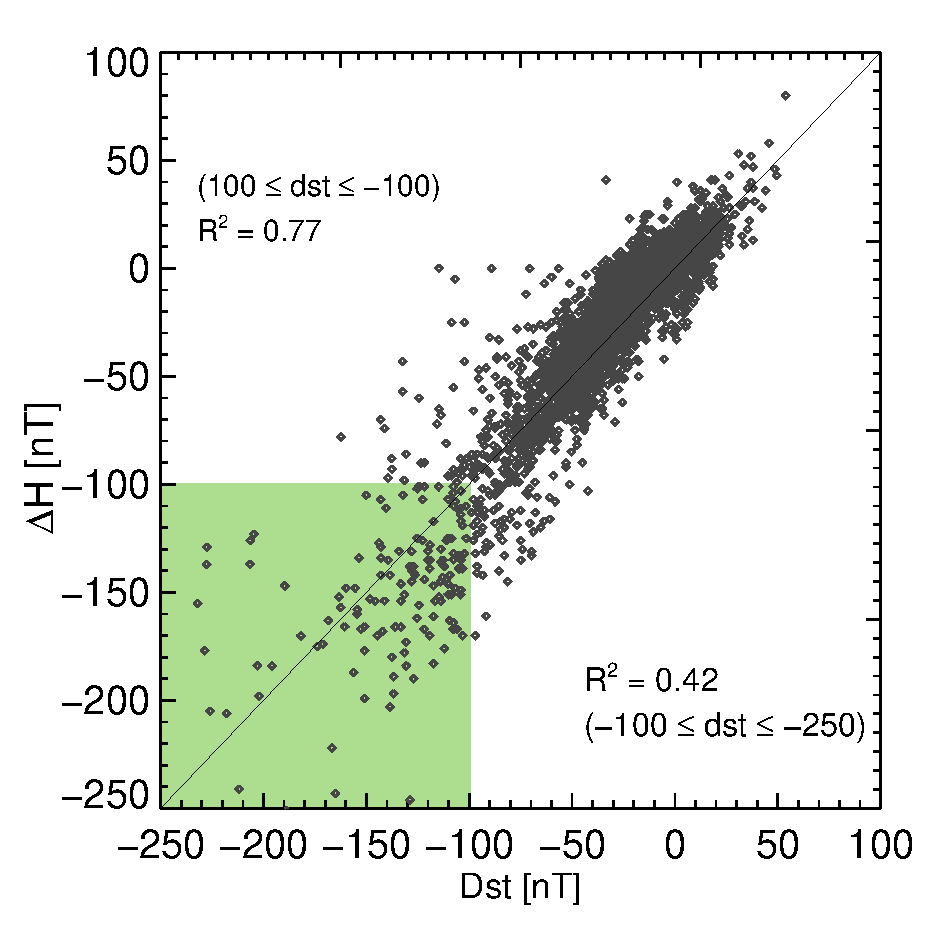
\includegraphics[width=0.45\textwidth]{images/disp_dst_v_dh/dispersion_general_dst.eps}
      \caption{Dispersion plot of $\Delta$H (vertical axis) with respect to Dst (horizontal axis) for all GS events. The green region represents a -100 nT threshold in which it was computed a second $R^2$.}
       \label{fig:disp}
\end{figure}


\subsection{Geomagnetic signatures of local ionospheric currents}
\label{diono}

The local values of the Earth's magnetic field (EMF) result from the combined contributions of various sources \citep{1969intro_to_iono_p, l_handbook_geof_sw_Geom_field, baseline_Gjerloev, vanKampt}. Specifically, for the horizontal component (H) of the local EMF, it can be expressed as follows:
\begin{equation}
    \label{eq:1}
    H = B_{SQ} + H_0 + D_{M} + D_{I},
\end{equation}
Here, $B_{SQ}$ represents the diurnal variation derived from local quiet days \citep{vanKampt}, while $H_0$ captures the day-to-day variations \citep{baseline_Gjerloev}. The final two terms, $D_{M}$ and $D_{I}$, correspond to irregular magnetic variations associated with geomagnetic activity \cite{ddyn2005, angeoddyn}. Specifically, $D_{M}$ accounts for contributions from planetary-scale magnetospheric currents, while $D_{I}$ is linked to magnetic perturbations caused by ionospheric disturbances. Notably, for mid and low latitudes, $D_{M}$ can be approximated by $Dst \cdot \cos(\lambda)$, where $\lambda$ is the geomagnetic latitude \citep{amorymazaudier_2017}. This approximation simplifies Equation \ref{eq:1} to:
\begin{equation}
\label{eq:diono}
   D_{I} \approx H -(B_{SQ} +  H_0 + Dst \cdot cos(\lambda)).
\end{equation}

Furthermore, $D_{I}$ can be decomposed into individual components as follows:
\begin{equation}
\label{eq:diono_explicit}
   D_{I} = DP2 + Ddyn + D_{others},
\end{equation}
Here, $D_{others}$ refers to ionospheric perturbations distinct from $DP2$ and $Ddyn.$

To effectively isolate the magnetic signatures attributed to $DP2$ and $Ddyn$ in Equations (\ref{eq:diono}) and (\ref{eq:diono_explicit}), we will employ frequency filters to analyze $D_{I}$ \citep{amory2020_filtros}. These filters will be designed based on the frequency range (periods) associated with magnetic fluctuations induced by each current in the local EMF. Specifically, it is established that the magnetic fluctuations induced by $Ddyn$ exhibit primary periods of approximately $24\, {\rm h}$. In contrast, the oscillation periods of fluctuations induced by $DP2$ are equal to or less than $4\, {\rm h}$ \cite{blanc_ddyn, angeoddyn}. As a result, the filters employed will be a pass-band filter for $DP2$ and a high-pass filter for $Ddyn$ \citep{nishida_68_fluctuations, blanc_ddyn}.



% ---------------------------------------------------
% ---------->    SECTION    <----------
% ---------------------------------------------------
\section{Analysis and results}
\label{results}

\subsection{Local ionospheric disturbances and induced magnetic fluctuations}
\label{analysis}
In this section, we present our analysis process through analyzing event 13. The panel (a) of Figure \ref{fig:iono_resp} shows the profiles of $Dst$ (black) and $\Delta H$ (green) indices during the GS associated with event 13 (see Table \ref{table1:GS_descp}). In the panel, we observe that both indices are \emph{quiet} up to the start of the GS's main phase, signed out by a vertical dotted line. The main phase lasts approximately one day, reaching a minimum of $Dst \sim -300\,{\rm nT}$, whereas the recovering phase extends almost three days. 

\begin{figure*}
\centering
    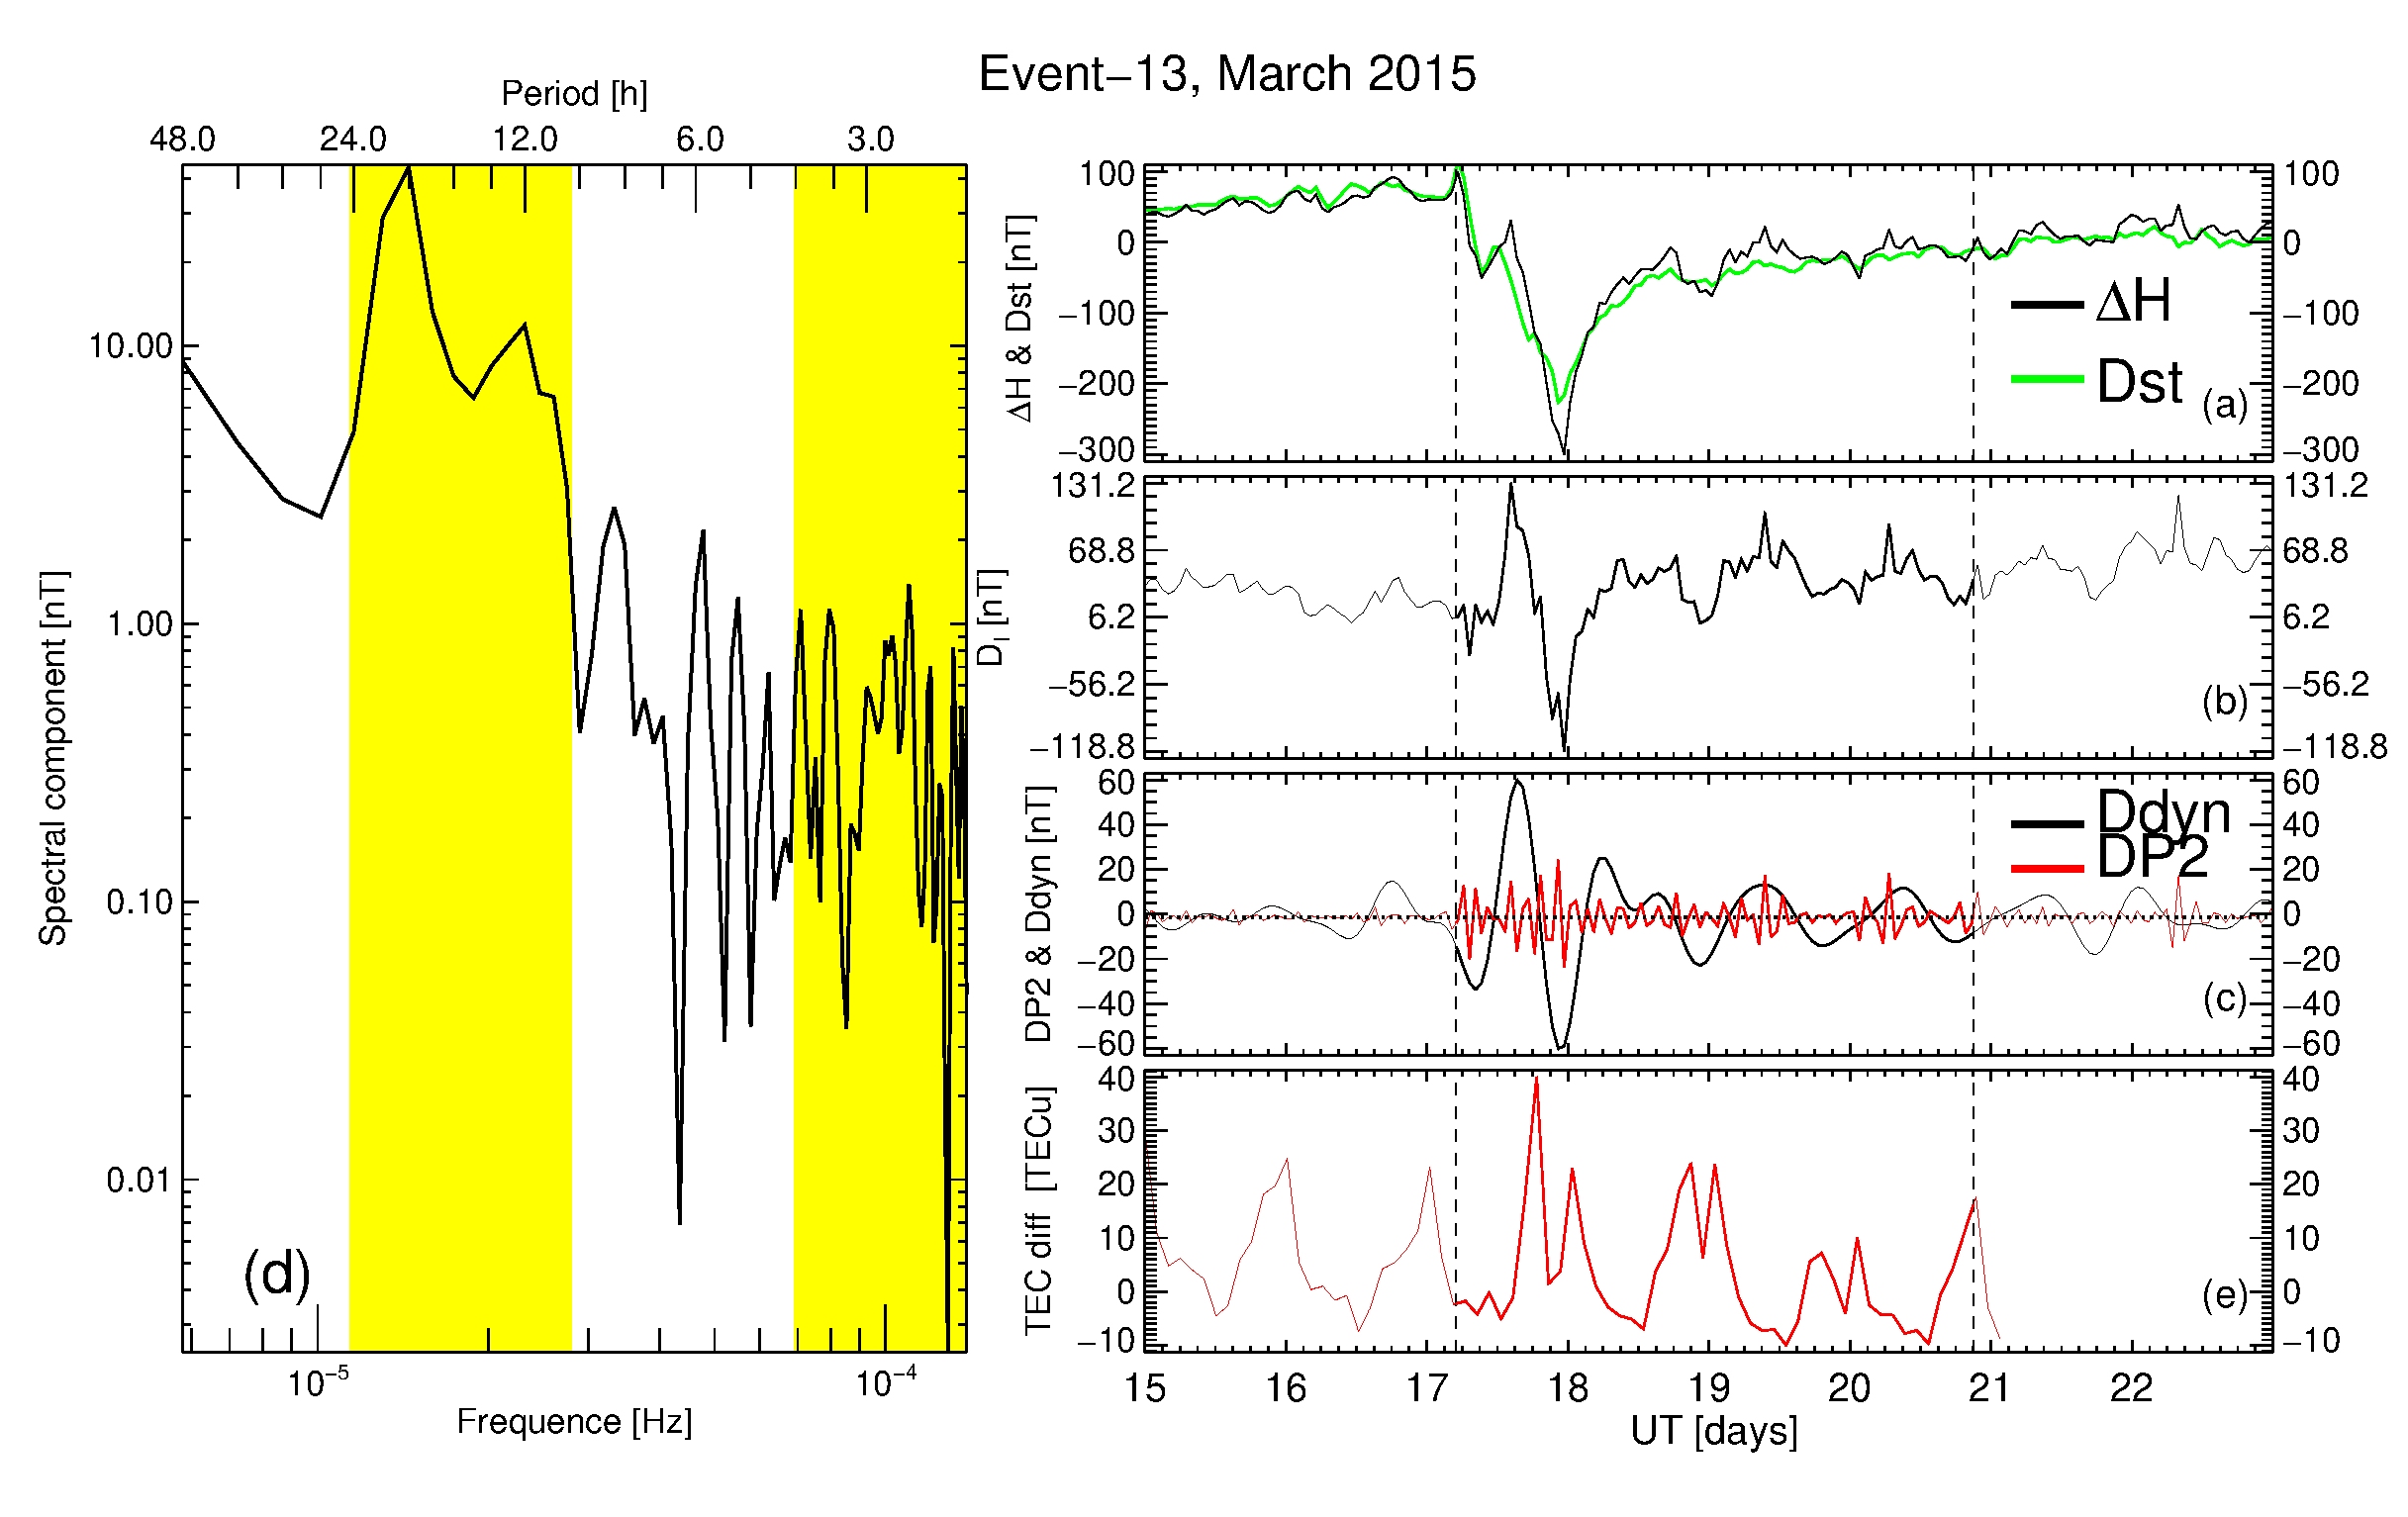
\includegraphics[width=0.85\textwidth]{images/diono/iono_PI_2015-03-15.eps}
    \caption{Analysis of study case 13. Panel (a): $Dst$ (black) and $\Delta H$ (green). Panel (b): computed value of $D_I$. Panel (c): Reconstructed profiles of the induced geomagnetic effects of Ddyn (black line) and DP2 (red line). Panel (d): Power spectrum of $D_I$. Panel (e): Measured total electron content (TEC) over the center of Mexico. Dotted vertical lines mark out GS's start (left) and end (right). Yellow shadowing regions in panel (d) highlight the bandwidths associated with $Ddyn$ (25h - 10 h) and $DP2$ (less than 4.5 h) filters.}
    \label{fig:iono_resp}
\end{figure*}

In the panel (b) of Figure \ref{fig:iono_resp}, we appreciate the resulting profile of $D_I$ (Equation (\ref{eq:diono})), which we computed using the TEO's registers and the $Dst$ reported data. Subsequently, we construct a power spectrum for our computed profile of $D_I$, which we show in panel (d) of Figure \ref{fig:iono_resp}. In the power spectrum, we highlight, by a yellow shadowing, the range of periods(frequencies) consistent with $DP2$ and $Ddyn$. In the panel, we identify $Ddyn$'s range by setting the main period and searching potency peaks within the range of possible harmonics. It is important to remark that, because our study cases might be potentially different from each other, the filtering ranges might vary slightly from case to case.

In Figure \ref{fig:iono_resp}(c) we present the profiles of the induced magnetic perturbations caused by $DP2$ (solid red line) and $Ddyn$ (solid black line). These profiles are constructed departing from the frequencies identified through the filtering process commented on in the previous paragraph. We note that the enhancements of the induced effects of $Ddyn$ and $DP2$ simultaneously occur with an increase in the total electron content over central Mexico, as the panel (e) of Figure \ref{fig:iono_resp} shows.
 
We applied the procedure presented in this section to all our study cases. The Figures \ref{fig:iono_resp2} and \ref{fig:iono_resp3} in the Appendix show the computed $D_I$ and the resulting profiles of $DP2$ and $Ddyn$, for each event in Table \ref{table1:GS_descp}. We remark on the uniqueness of each event, which is clear in the $D_I$ profiles and its associated magnetic perturbations induced by $DP2$ and $Ddyn$ currents.

From Figures \ref{fig:iono_resp2} and \ref{fig:iono_resp3}, we note that generally, the amplitude of the magnetic oscillations induced by $Ddyn$ are more intense than those induced by $DP2$. This suggests that, in most cases, $Ddyn$'s induced magnetic effects are dominant on the local EMF. Although there are events for which both effects show similar intensities. We think of two possibilities to explain that: The first is the process that triggers the GS itself, \emph{i.t.} the solar activity event, and its magnetic reconnection with the EMF. This may affect the evolution of the ionospheric response, directly modifying the evolution of $DP2$ and $Ddyn$ currents. Secondly, we have to consider that our data is sampled in hourly resolution. In this case, data sampling represents an important limitation since $DP2$ magnetic fluctuations, as mentioned in \cite{nishida_68_fluctuations}, may have periods of less than an hour or even of tens of minutes. In this scenario, we possibly missed part of $DP2$ fluctuations during our analysis. This could be solved, in principle, by using $Sym-H$ index rather than $Dst$, a task in which exploration we consider our future work.


\subsection{Validation of DP2 and Ddyn magnetic signatures}
\label{validation}

In Section \ref{local response}, we identified substantial differences between planetary and regional geomagnetic activity, attributing these distinctions to regional geomagnetic responses. In Section \ref{analysis}, we pinpointed the tentative geomagnetic mechanisms behind these responses—namely, the $Ddyn$ and $DP2$ ionospheric currents—by employing a process of frequency filtering. Furthermore, we established that these effects correlate systematically with local Total Electron Content (TEC) perturbations. To validate these findings, a multi-step approach is necessary.

Initially, we approximate the regional geomagnetic index $\Delta H$ by defining it as follows:
\begin{equation}
    \label{eq:deltaH}
    \Delta H = H - (B_{SQ} + H_0),
\end{equation}
Using Equations (\ref{eq:diono}), (\ref{eq:diono_explicit}), and (\ref{eq:deltaH}), we derive:
\begin{equation}
    \label{eq:deltaHandDst}
    \Delta H \approx Dst \cos(\lambda) + DP2 + Ddyn.
\end{equation}
To simplify, we denote $ Dst_\lambda$ as the combined effect of $ Dst\cos(\lambda)$, $DP2$, and $Ddyn$. This leads to our first validation step, confirming whether the computed $ Dst_\lambda$ approximates $\Delta H$. Additionally, we employ $ Dst_\lambda$ and the values of $K_p$ to approximate the local $K$ value.

Figure \ref{fig:iono_valid} portrays the validation process applied to event 13. The top panel juxtaposes profiles of $\Delta H$ (black), $Dst$ (green), and $Dst_\lambda$ (red). It is evident that $Dst_\lambda$ consistently tracks closer to $\Delta H$ than $Dst$, holding true during the main and recovery phases of the geomagnetic storm (GS). The bottom panel reveals that the values of planetary (green) and local (black) $K$ differ. However, when $Dst_\lambda$ is combined with $K_p$ values using uncertainty bars, the local $K$ profile generally falls within this range.

\begin{figure}
\centering
    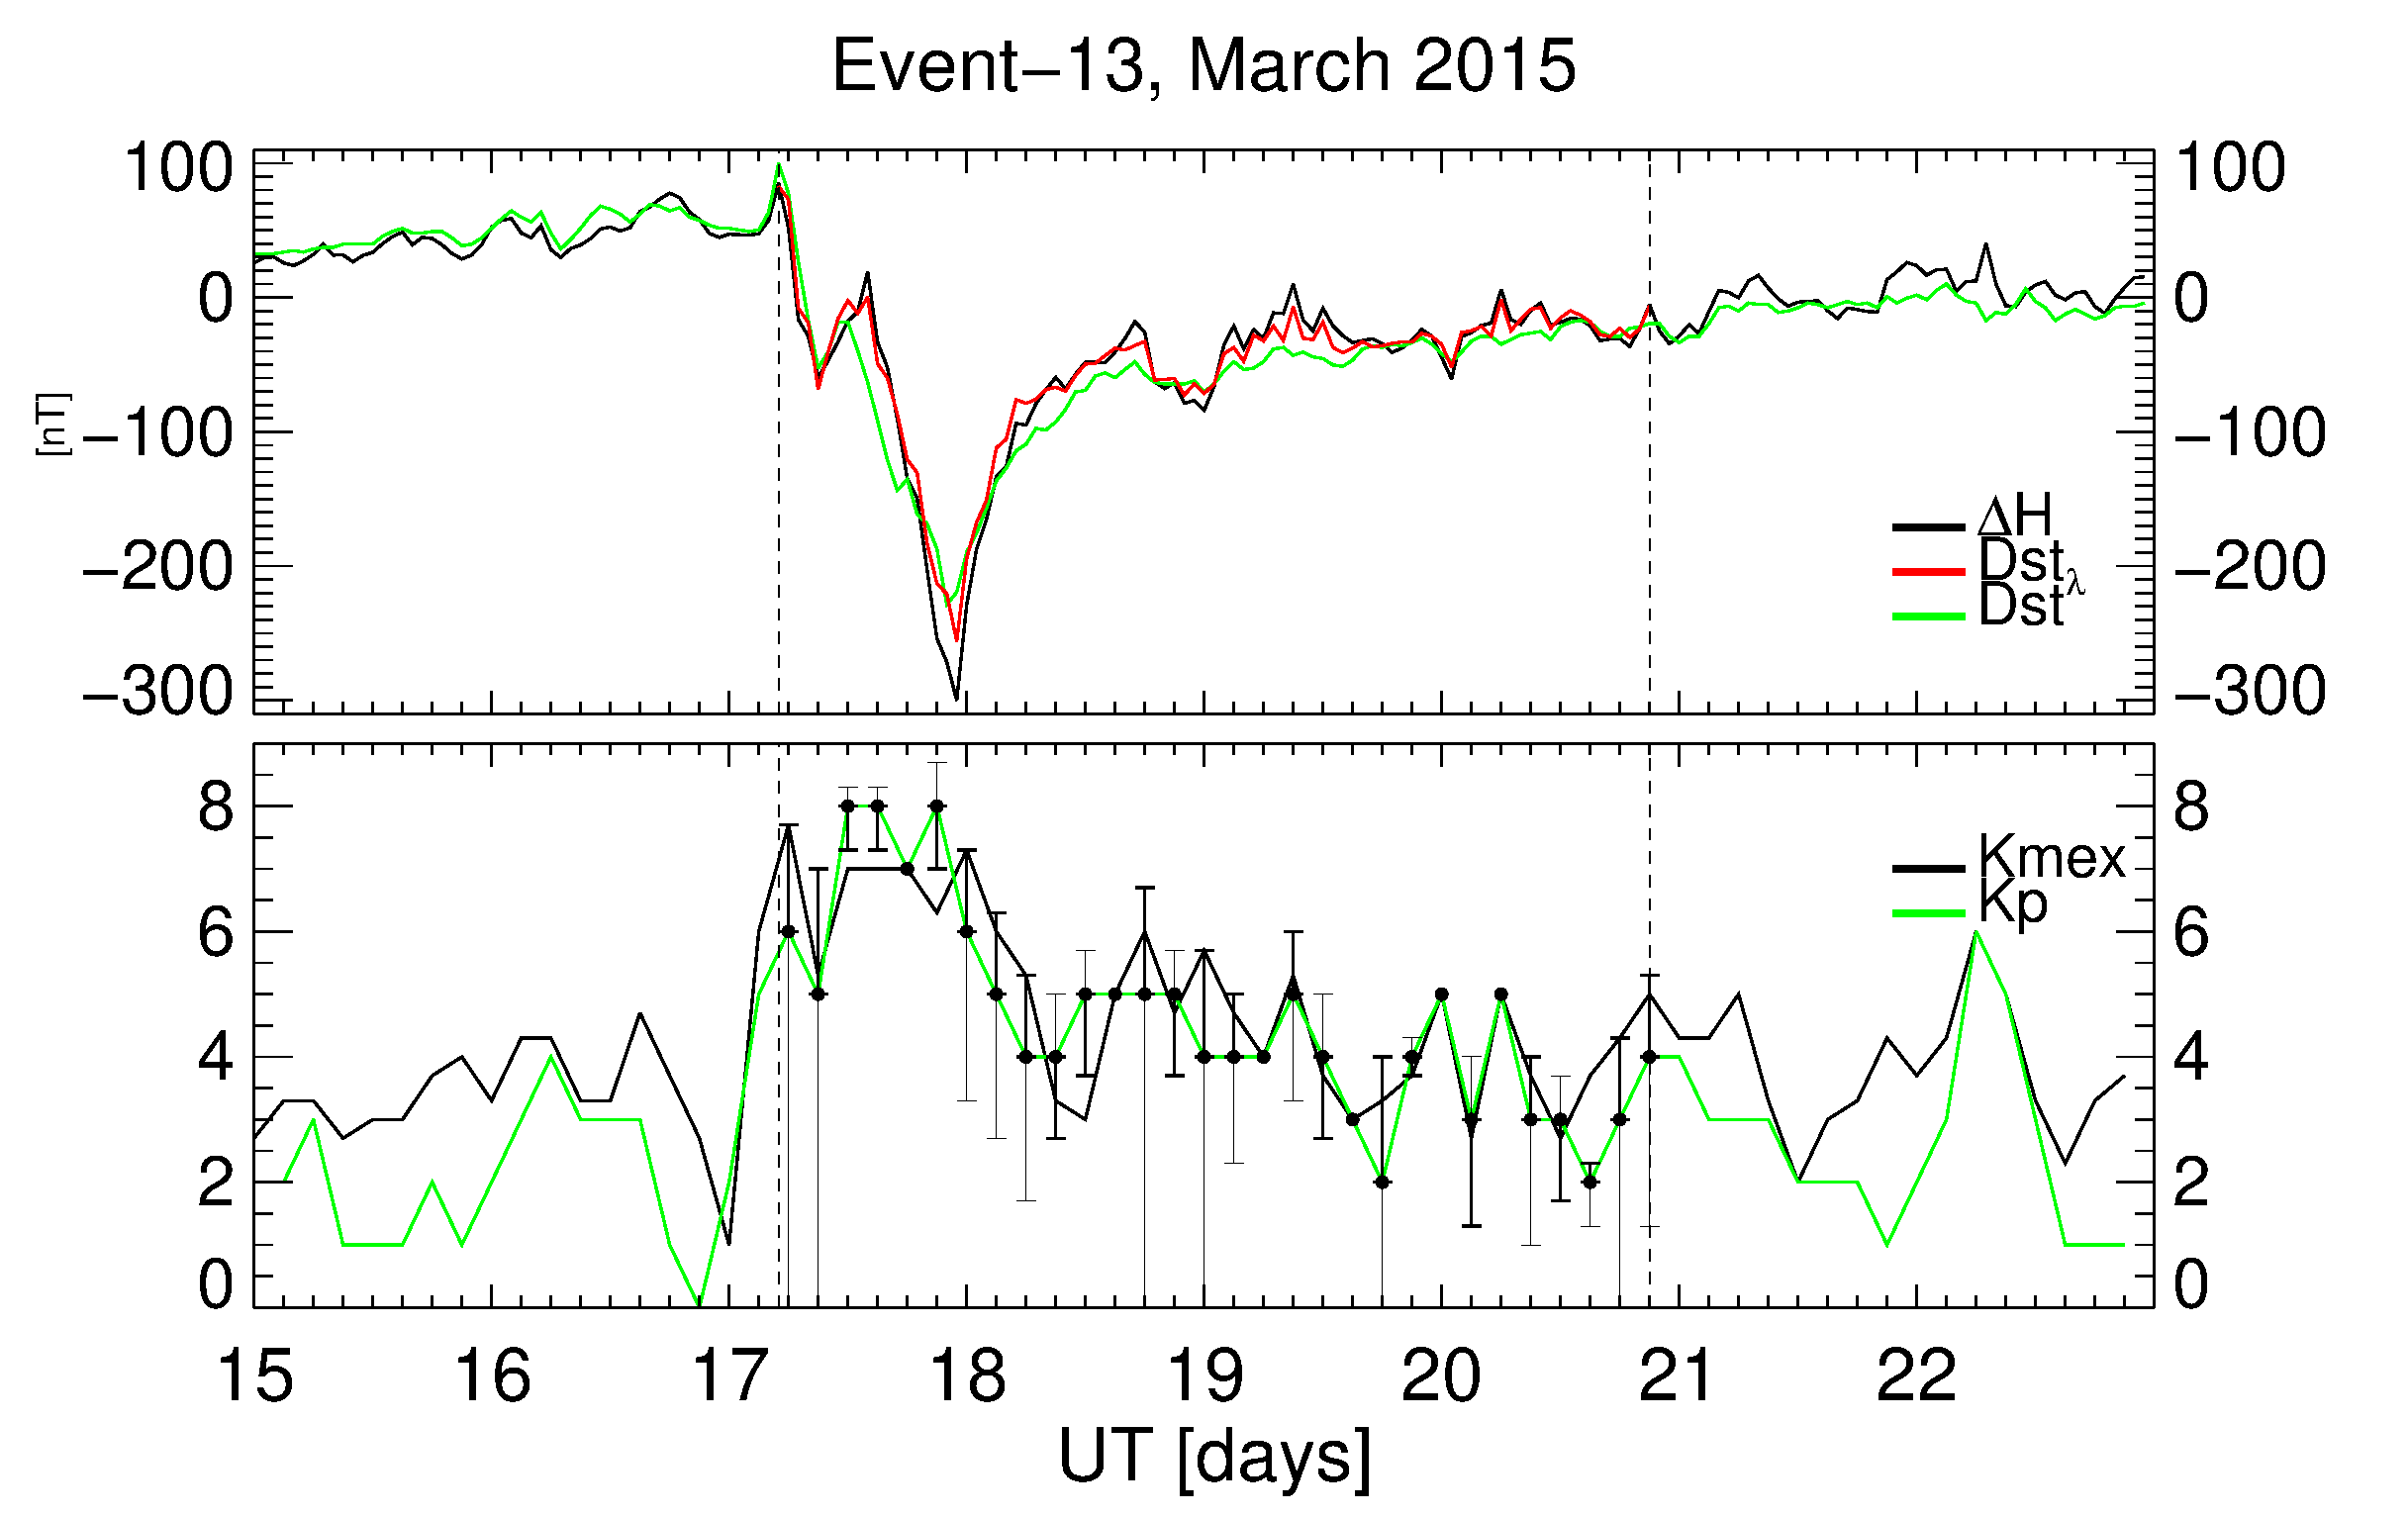
\includegraphics[width=0.45\textwidth]{images/dH_approx/diono_valid_V4_2015-03-15.eps}
    \caption{Approximation of $\Delta$H (top) and local K (bottom) geomagnetic indices. The green solid lines represent planetary indices and black solid lines represents local geomagnetic indices. The approximated $\Delta$H index is represented by the red line while the error bars represent an approximation range for Kmex index.}
    \label{fig:iono_valid}
\end{figure}

To validate comprehensively, this process is applied to all studied cases. Figures \ref{fig:iono_valid2} and \ref{fig:iono_valid3} showcase the results. Consistently, $ Dst_\lambda$ approximates $\Delta H$, and $K_p$ with the effects of $Dst_\lambda$ encapsulates regional $K$ values.

Additionally, a quantitative assessment is conducted. The average absolute differences between $\Delta H$-$Dst$ and $\Delta H$-$Dst_\lambda$ pairs across the study cases are computed. As displayed in Figure \ref{fig:valid}, the histogram illustrates the average differences between $\Delta H$-$Dst$ (blue bars) and $\Delta H$-$Dst_\lambda$ (red bars). Notably, the average difference associated with $Dst_\lambda$ consistently outperforms that of $Dst$, implying the relevance of magnetic perturbations corresponding to $DP2$ and $Ddyn$ for regional geomagnetic responses.

\begin{figure}
\centering
    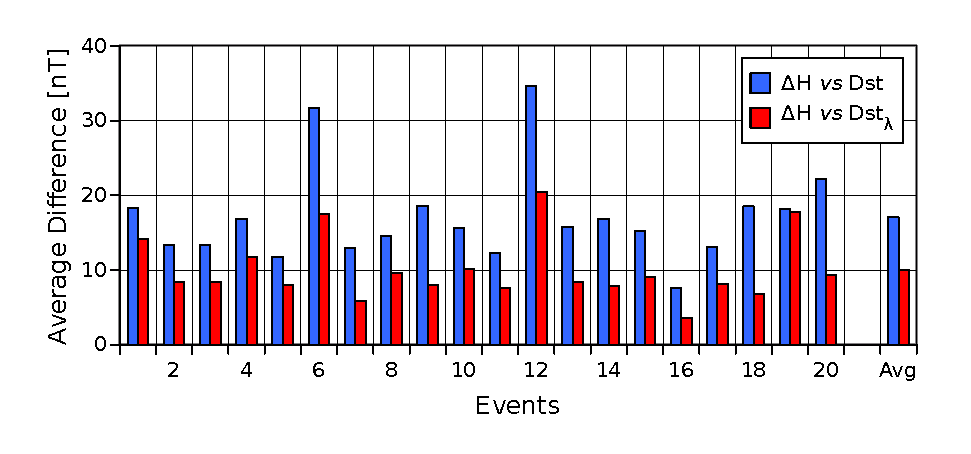
\includegraphics[width=0.45\textwidth]{images/prom_dist.eps}
    \caption{Average error (Top) measured in nT between $\Delta$H vs Dst and $\Delta$H vs $Dst_\lambda$. Error difference (bottom) between the two cases above.}
    \label{fig:valid}
\end{figure}

The final step involves remaking the dispersion plot from Figure \ref{fig:disp}, employing $Dst_\lambda$ data instead of $Dst$. The resulting Figure \ref{fig:valid_disp2} depicts data points (open diamonds) closely following the identity (solid black line), in contrast with Figure \ref{fig:disp}. Moreover, $R^2$ improves from 0.77 to 0.86 for $Dst \ge -100\, {\rm nT}$, and for $Dst < -100\, {\rm nT}$, $R^2$ rises to 0.75, a significant increase from the original $Dst$ value ($R^2=0.42$).

\begin{comment}
\begin{table*}[h!]
\normalsize
\centering
    \begin{tabular}{|c|c|c|c|}
        \hline
No. Event & \multicolumn{1}{c|}{$\frac{\delta-\delta_{DP2}}{\delta}$} & \multicolumn{1}{c|}{$\frac{\delta - \delta_{Ddyn}}{\delta}$} & \multicolumn{1}{c|}{$\frac{\delta - \delta_\lambda}{\delta}$} \\ 
  & \multicolumn{1}{c|}{[$\%$]} & \multicolumn{1}{c|}{[$\%$]} & \multicolumn{1}{c|}{[$\%$]} \\ \hline

SG-1 & 17.32 & 21.15 & 22.62 \\ \hline
SG-2 & 8.91 & 30.11 & 37.00 \\ \hline
SG-3 & 8.91 & 30.11 & 37.00 \\ \hline
SG-4 & -6.16 & 23.87 & 30.51 \\ \hline
SG-5 & 12.01 & 31.69 & 32.03 \\ \hline
SG-6 & 0.25 & 35.08 & 44.70 \\ \hline
SG-7 & 30.85 & 47.67 & 54.42 \\ \hline
SG-8 & 12.52 & 32.94 & 34.11 \\ \hline
SG-9 & 23.76 & 42.62 & 56.79 \\ \hline
SG-10 & 27.49 & 32.93 & 35.23 \\ \hline
SG-11 & 7.74 & 37.65 & 38.06 \\ \hline
SG-12 & 16.49 & 39.16 & 40.77 \\ \hline
SG-13 & 6.46 & 40.81 & 46.77 \\ \hline
SG-14 & 20.23 & 47.27 & 53.08 \\ \hline
SG-15 & 7.28 & 32.87 & 40.16 \\ \hline
SG-16 & 12.73 & 49.08 & 52.89 \\ \hline
SG-17 & 15.50 & 35.50 & 38.02 \\ \hline
SG-18 & 9.94 & 53.16 & 63.10 \\ \hline
SG-19 & -27.25 & -1.88 & 1.88 \\ \hline
SG-20 & 12.96 & 56.66 & 57.92 \\ \hline
Avr & 10.90 & 35.92 & 40.85 \\ \hline
    \end{tabular}
    \caption{Average distance reduction percentage of each GS event (first column) considering DP2 effect (second column), Ddyn effect (third column) and both (fourth column). }
    \label{table2:valid}
\end{table*}
\end{comment}


\begin{figure}
    \centering
     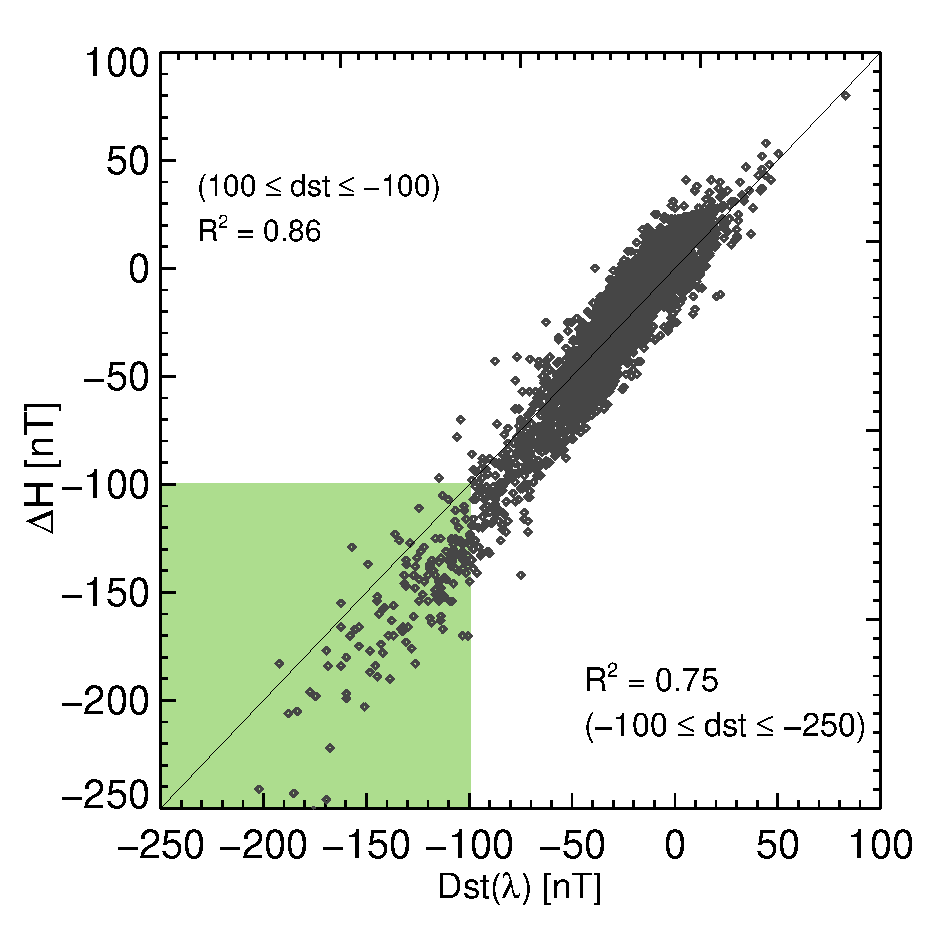
\includegraphics[width=0.45\textwidth]{dispersion_general_dst_ld.eps}
      \caption{Dispersion plot of $\Delta H$ (vertical axis) with respect to $Dst_\lambda$ (horizontal axis) for all GS events. The green region represents a -100 nT threshold in which it was computed a second $R^2$.}
       \label{fig:valid_disp2}
\end{figure}

Our validation process proved that the magnetic perturbations tentatively induced by $DP2$ and $Ddyn$ ionospheric currents, when combined with planetary indices, allowed to qualitatively approximate the regional geomagnetic activity. We also proved that regional geomagnetic response, as registered by $\Delta H$, can be quantitatively expressed by the planetary response ($Dst$) combined with the geomagnetic effects of the already commented ionospheric currents. Finally, when including the magnetic effects induced by $DP2$ and $Ddyn$ into the planetary response, the dispersion between regional and planetary data substantially decreased.

Through this validation process, we successfully demonstrate that the magnetic perturbations potentially induced by $DP2$ and $Ddyn$ ionospheric currents, when combined with planetary indices, allow for qualitative and quantitative approximations of regional geomagnetic activity. Furthermore, the disparity between regional and planetary data is substantially reduced by integrating the magnetic effects resulting from $DP2$ and $Ddyn$ into the planetary response.

\section{Concluding remarks}

In this work, we studied the regional manifestations of space weather. We focused on the differences between planetary and local geomagnetic responses during periods of strong geomagnetic storms (GS) at the center of Mexico. We also investigated the possible sources for such differences in the geomagnetic response. We used the geomagnetic registers from the Teoloyucan Magnetic Observatory (TEO), located north of Mexico City. We also use data sets from the $Dst$ and $K_P$ planetary indices, the regional geomagnetic index $\Delta H$, and the total electron content delivered by the Mexican Space Weather National Laboratory.

We selected 20 GS as study cases for this work (see Table \ref{table1:GS_descp}). For all our study cases, we identified evidence of relevant regional geomagnetic response through a dispersion plot (see Figure \ref{fig:disp}). In this regard, we found that in the range of $Dst < -100 {\rm nT}$, there is a tendency for the regional geomagnetic index to deviate from the planetary one. We assumed this as evidence for a regional geomagnetic response.

Subsequently, we isolated the geomagnetic effects due to ionospheric processes ($D_I$) from the regional (TEO) geomagnetic registers. Next, we applied filters on $D_I$ to identify the magnetic perturbations consistent with those induced by $Ddyn$ and $DP2$ currents. We also verified that intensifying the resulting $Ddyn$ and $DP2$ profiles simultaneously occurred during TEC perturbations (see discussion of Figure \ref{fig:iono_resp}). Consequently, we could reconstruct the regional geomagnetic response consistent with those induced by $Ddyn$ and $DP2$ currents.

Afterward, we validate our computed geomagnetic contribution due to $Ddyn$ and $DP2$ currents. First, we approximate the regional $K$ and $\Delta H$ indices by combining the planetary $K_P$ and $Dst$ indices with the regional geomagnetic effects of $Ddyn$ and $DP2$. Secondly, we computed the differences between $\Delta H$ and $Dst$ with and without the regional ionospheric effects. Finally, we analyzed the dispersion between $\Delta H$ and $Dst$ combined with the effects of $Ddyn$ and $DP2$. For all the cases, we found that regional geomagnetic response is qualitatively and quantitatively approximated by the geomagnetic planetary response combined with the geomagnetic perturbations induced by the $Ddyn$ and $DP2$ ionospheric currents. 

Finally, in this work, we focus on regional space weather. We identified evidence of a significantly different regional geomagnetic response from its planetary counterpart. We investigated $Ddyn$ and $DP2$ ionospheric currents as the mechanisms for such a regional response. As a result, we were able to isolate the magnetic perturbations associated with those ionospheric currents. Combining these perturbations with the planetary response could approximate the regional geomagnetic response.


% To print the credit authorship contribution details
\printcredits
\section*{Declaration of competing interest}
\label{Declaration}
The authors declare that they have no known competing financial interests or personal relationships that could have appeared to
influence the work reported in this paper.
%\section*{Funding}
%\label{funding}
%This research did not receive any specific grant from funding agencies in the public, commercial, or not-for-profit sectors.
\section*{Data Availability}
\label{data_A}
Data will be made available on request.
\section*{Acknowledgments}
P. Corona-Romero is grateful for Investigadores por M\'exico-CONAHCYT (CONAHCYT Research Fellow) project 1045 Space Weather Service, financed by “Consejo Nacional de Ciencia y Tecnolog\'ia” (CONAHCYT), which partially supported this work. C.I. Castellanos-Velazco is grateful for “La Beca de Posgrado en M\'exico” granted by CONAHCYT. LANCE acknowledges partial financial support from 
CONHACyT-AEM grant 2017-01-292684, CONAHCyT LN-315829, and PAPIIT IN116023.

This work used data from the Teoloyucan Magnetic Observatory operated by the Magnetic Service of the Geophysics Institute at the National and Autonomous University of Mexico (UNAM). Total electron content (TEC) and the geomagnetic indices $\Delta H$ and $K$, the regional counterparts of $Dst$ and $K_P$ indices, respectively, are produced by the Mexican Space Weather National Laboratory (LANCE), Geophysics Institute at National and Autonomous University of Mexico (UNAM).

The results presented in this paper rely on ${\rm K_{P}}$ and ${\rm Dst}$ geomagnetic indices calculated by the \href{https://www.gfz-potsdam.de/en/kp-index}{Helmholtz-Zentrum Potsdam Deutsches GeoForschungsZentrum Adolf-Schmidt-Observatorium} and the \href{https://wdc.kugi.kyoto-u.ac.jp/}{World Data Center for Geomagnetism, Kyoto}, respectively, from data collected at magnetic observatories. We thank the involved national institutes, the \href{https://intermagnet.github.io/}{INTERMAGNET network} and \href{https://isgi.unistra.fr}{ISGI}.

All authors have seen and approved the final version of the manuscript.  


\label{Ack}
%% Loading bibliography style file
%\bibliographystyle{model1-num-names}
\bibliographystyle{cas-model2-names}

% Loading bibliography database
\bibliography{ref.bib}

% Biography
\bio{}
% Here goes the biography details.
\endbio
%\bio{pic1}
% Here goes the biography details.
%\endbio


\section{Appendix}
\label{apend}
\begin{figure*}[h!]
    \centering
    \centerline{\Large \bf   
      %\hspace{0.18\textwidth}  \color{black}{\Large{Res}}
       %\hspace{0.28\textwidth}  \color{black}{\Large{Res+TC}}
         \hfill}
          \centerline{\Large \bf   
      \hspace{0.26\textwidth}  \color{black}{}
       \hspace{0.31\textwidth}  \color{black}{}
         \hfill}
     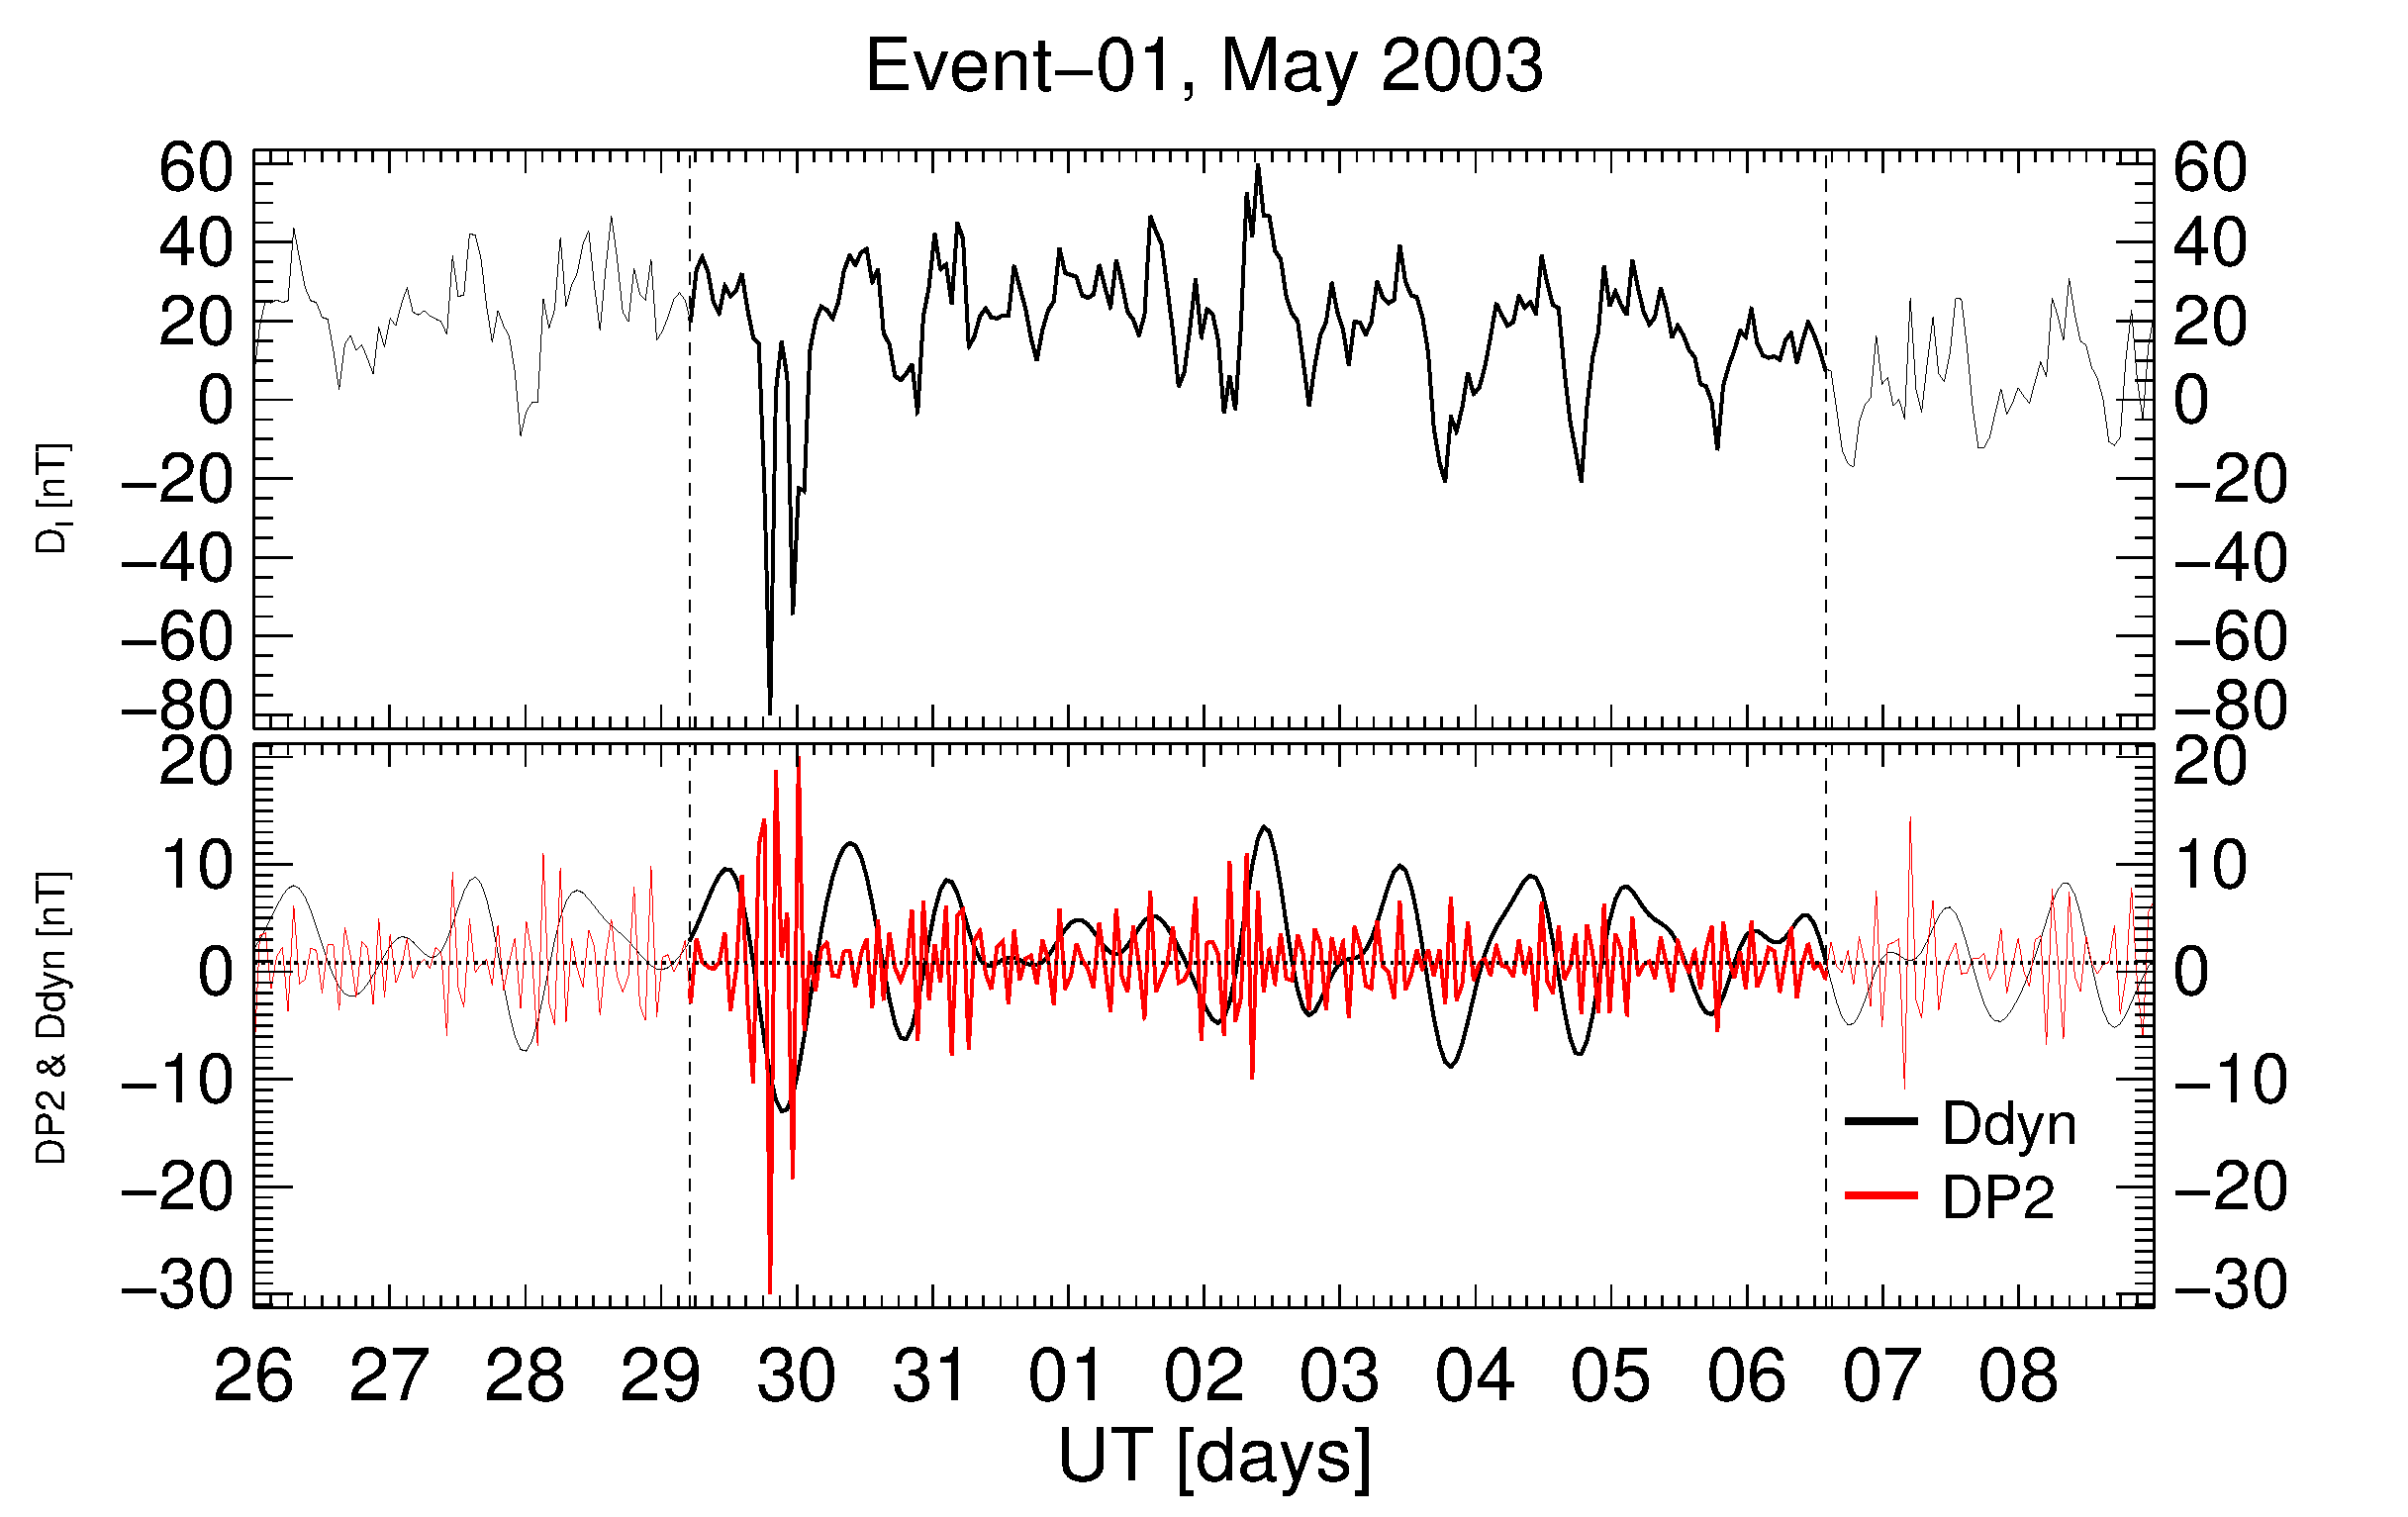
\includegraphics[width=6.0cm]{images/diono/iono_PI_V1_2003-05-26.eps}
     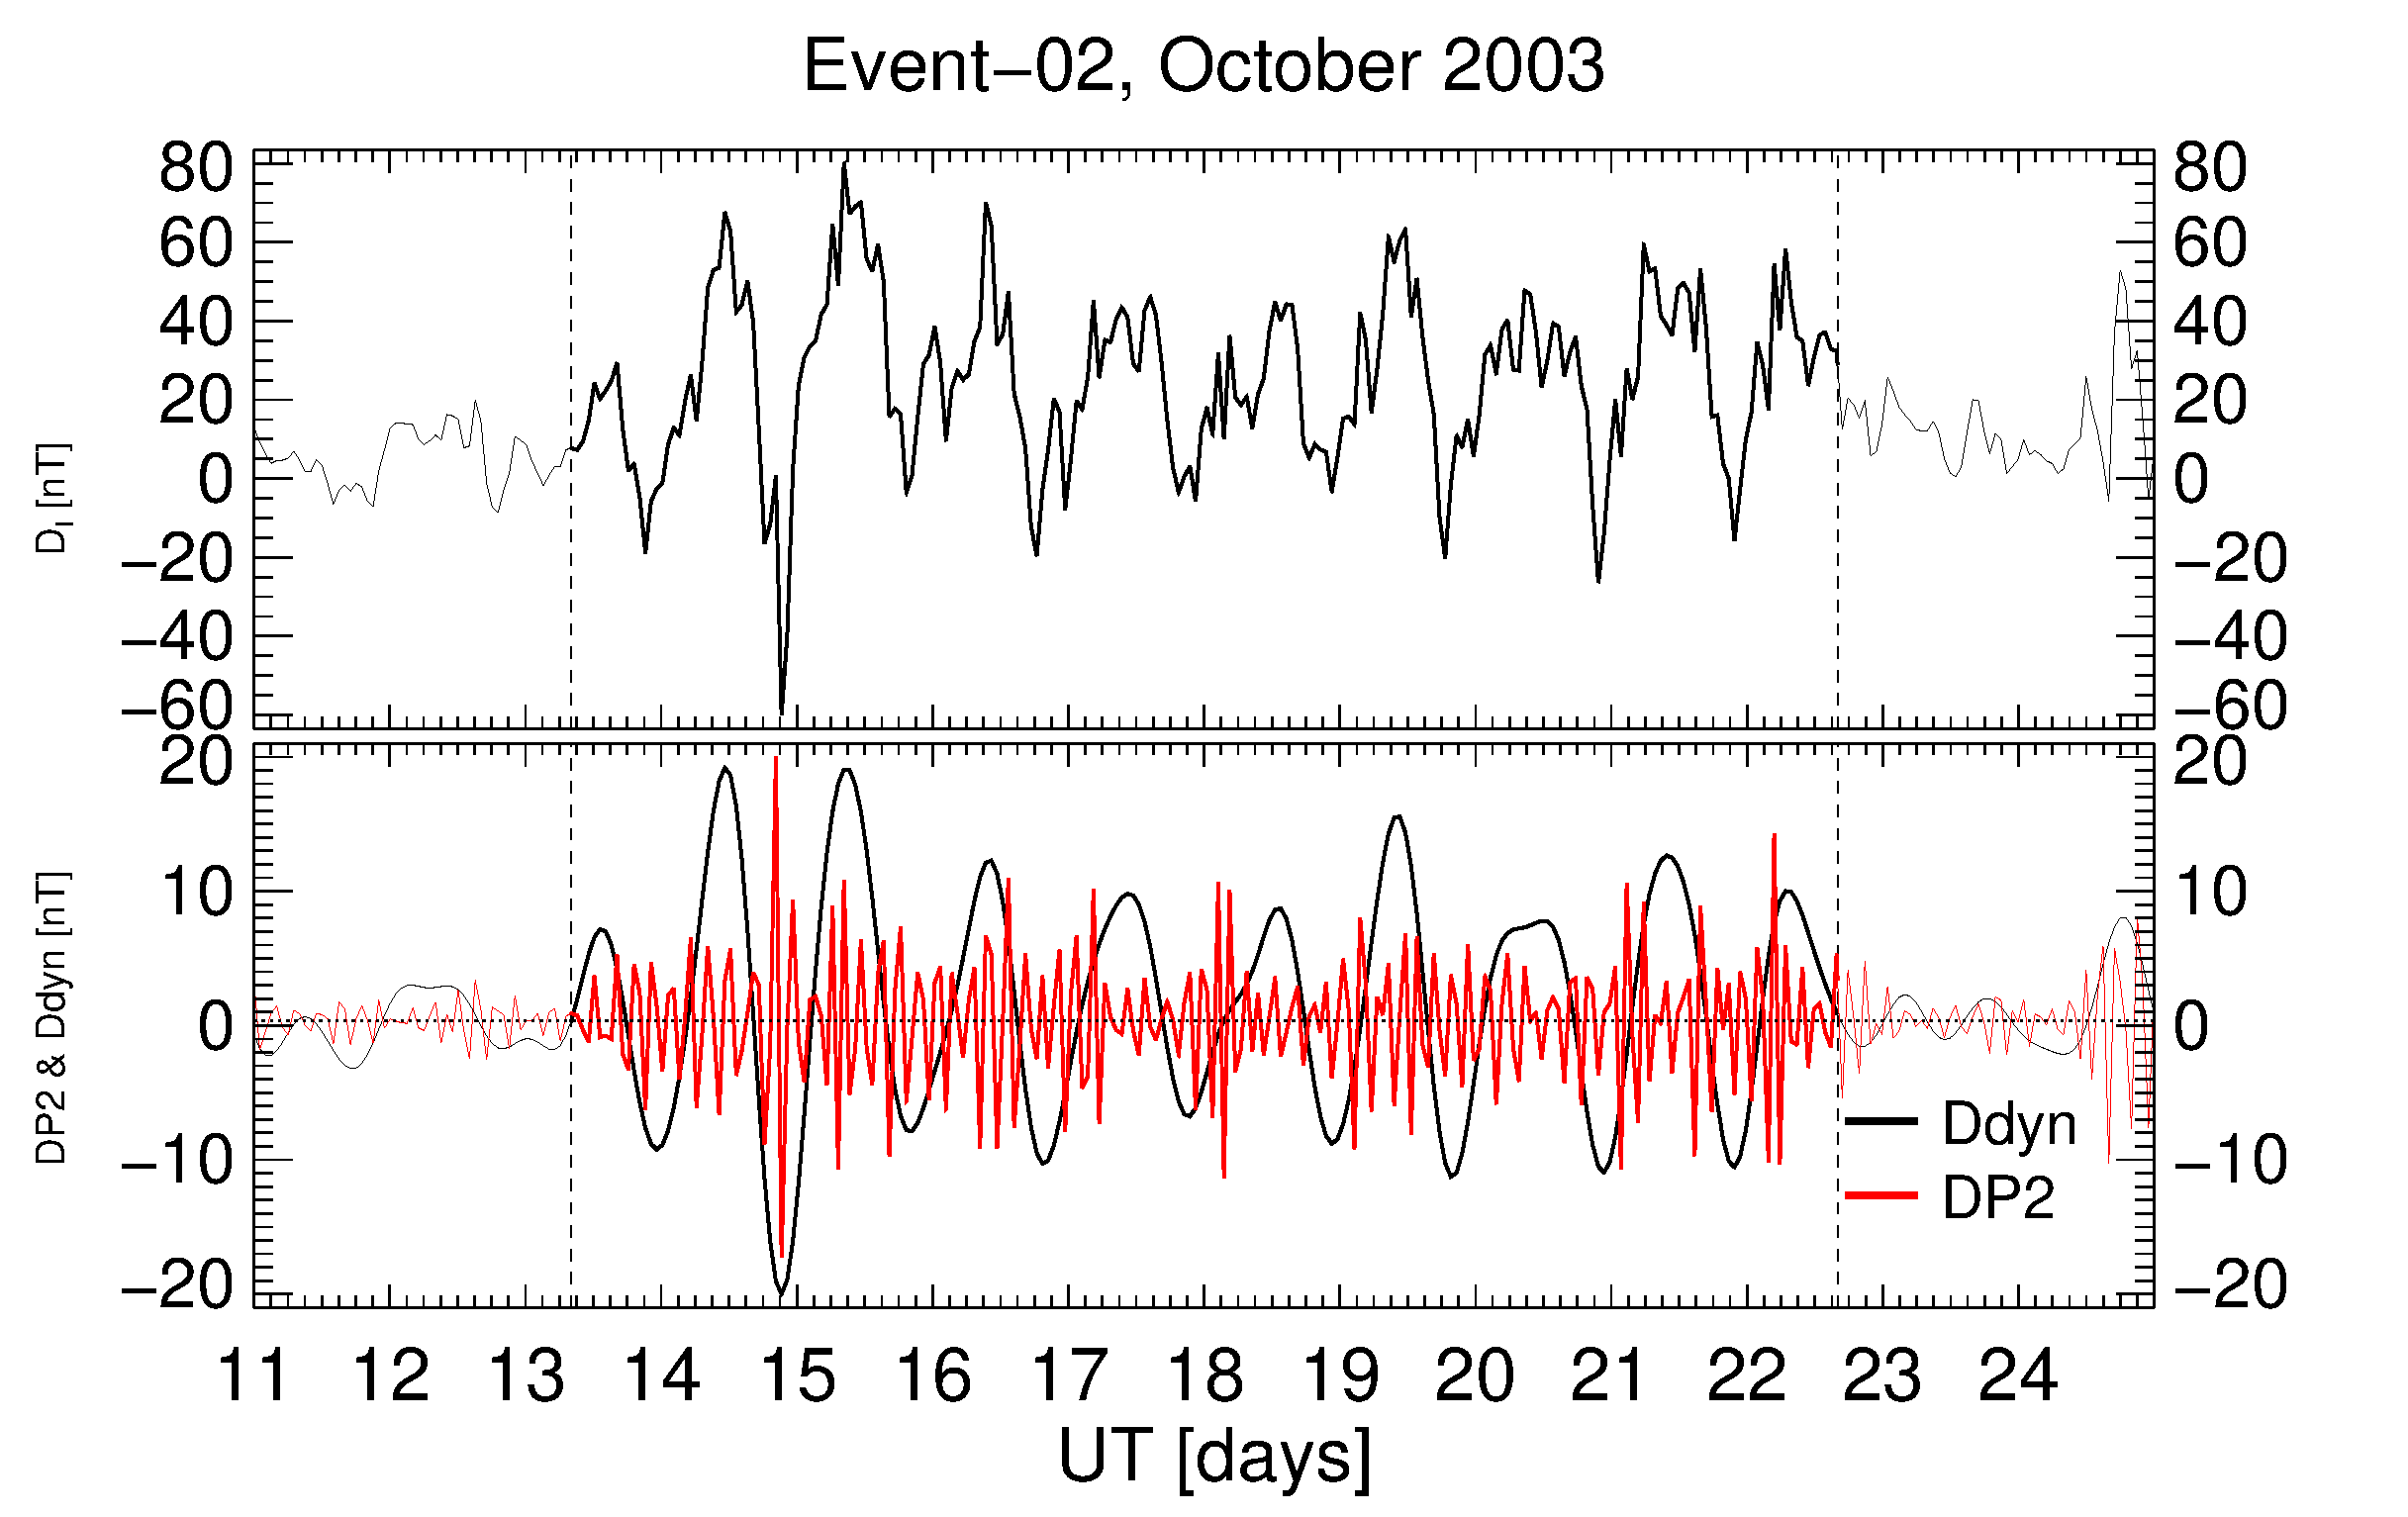
\includegraphics[width=6.0cm]{images/diono/iono_PI_V1_2003-10-11.eps}
     \centerline{\Large \bf   
      \hspace{0.275\textwidth}  \color{black}{}
       \hspace{0.295\textwidth}  \color{black}{}
         \hfill}
     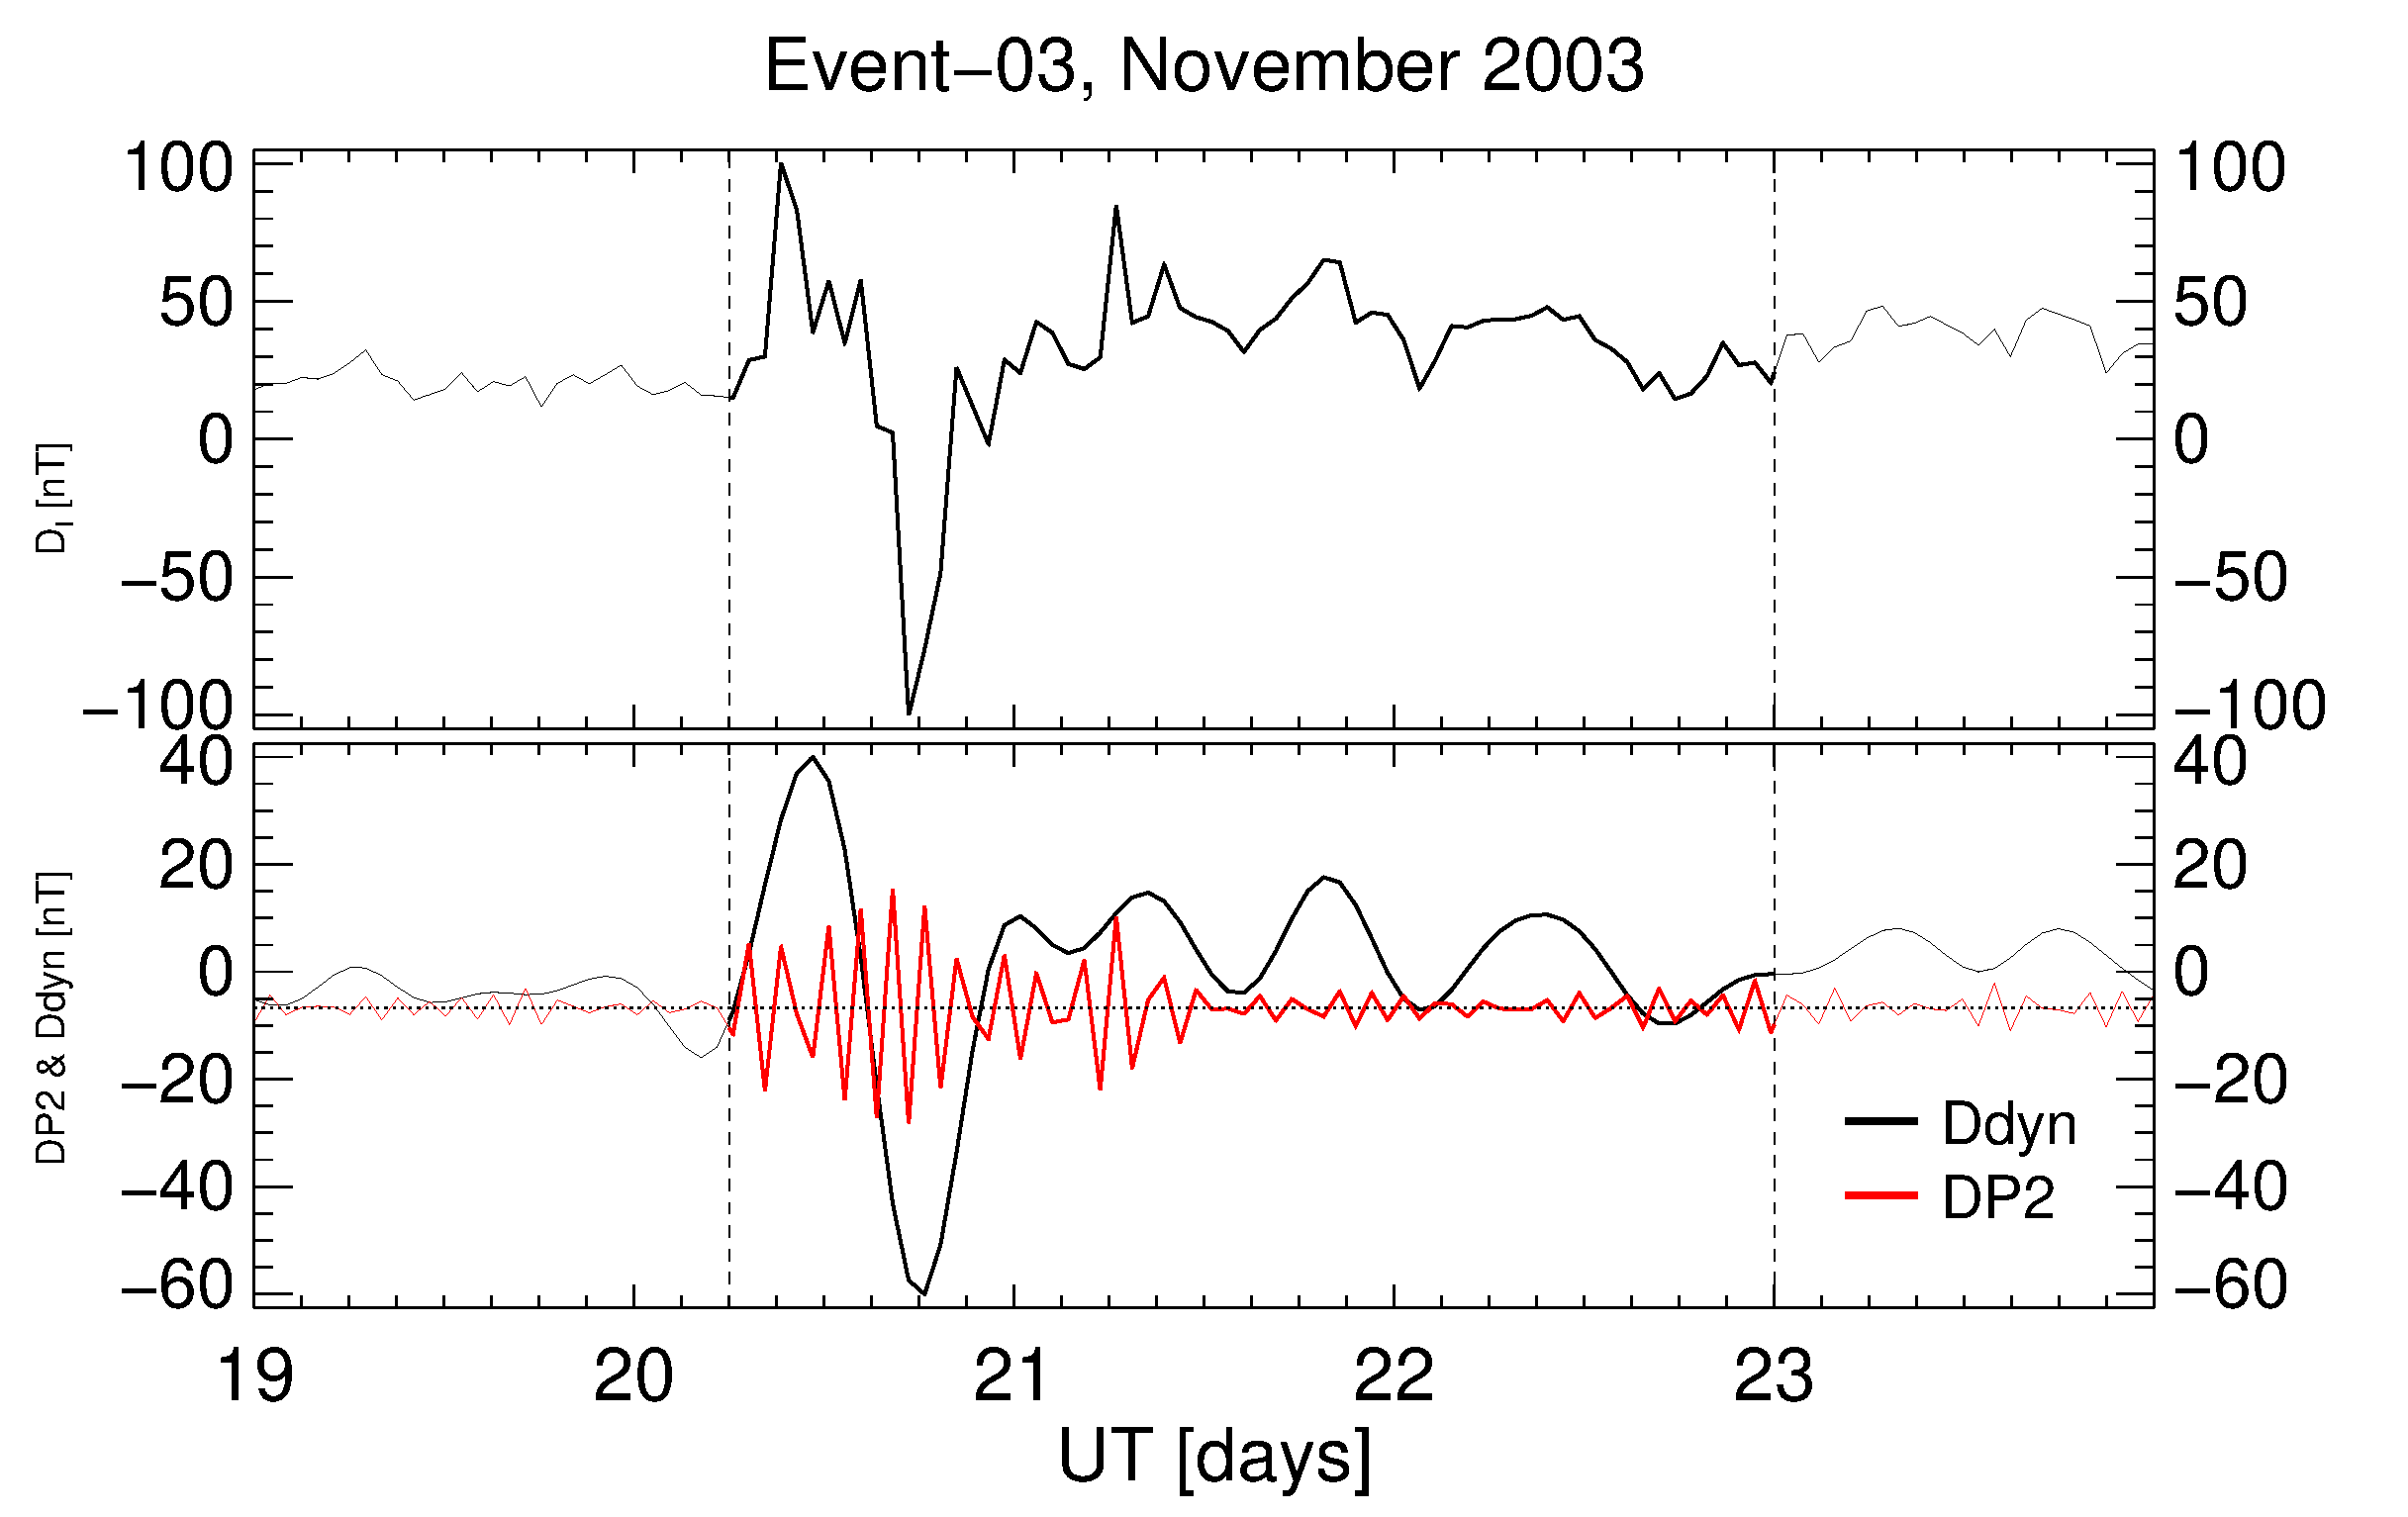
\includegraphics[width=6.0cm]{images/diono/iono_PI_V1_2003-11-19.eps}     
     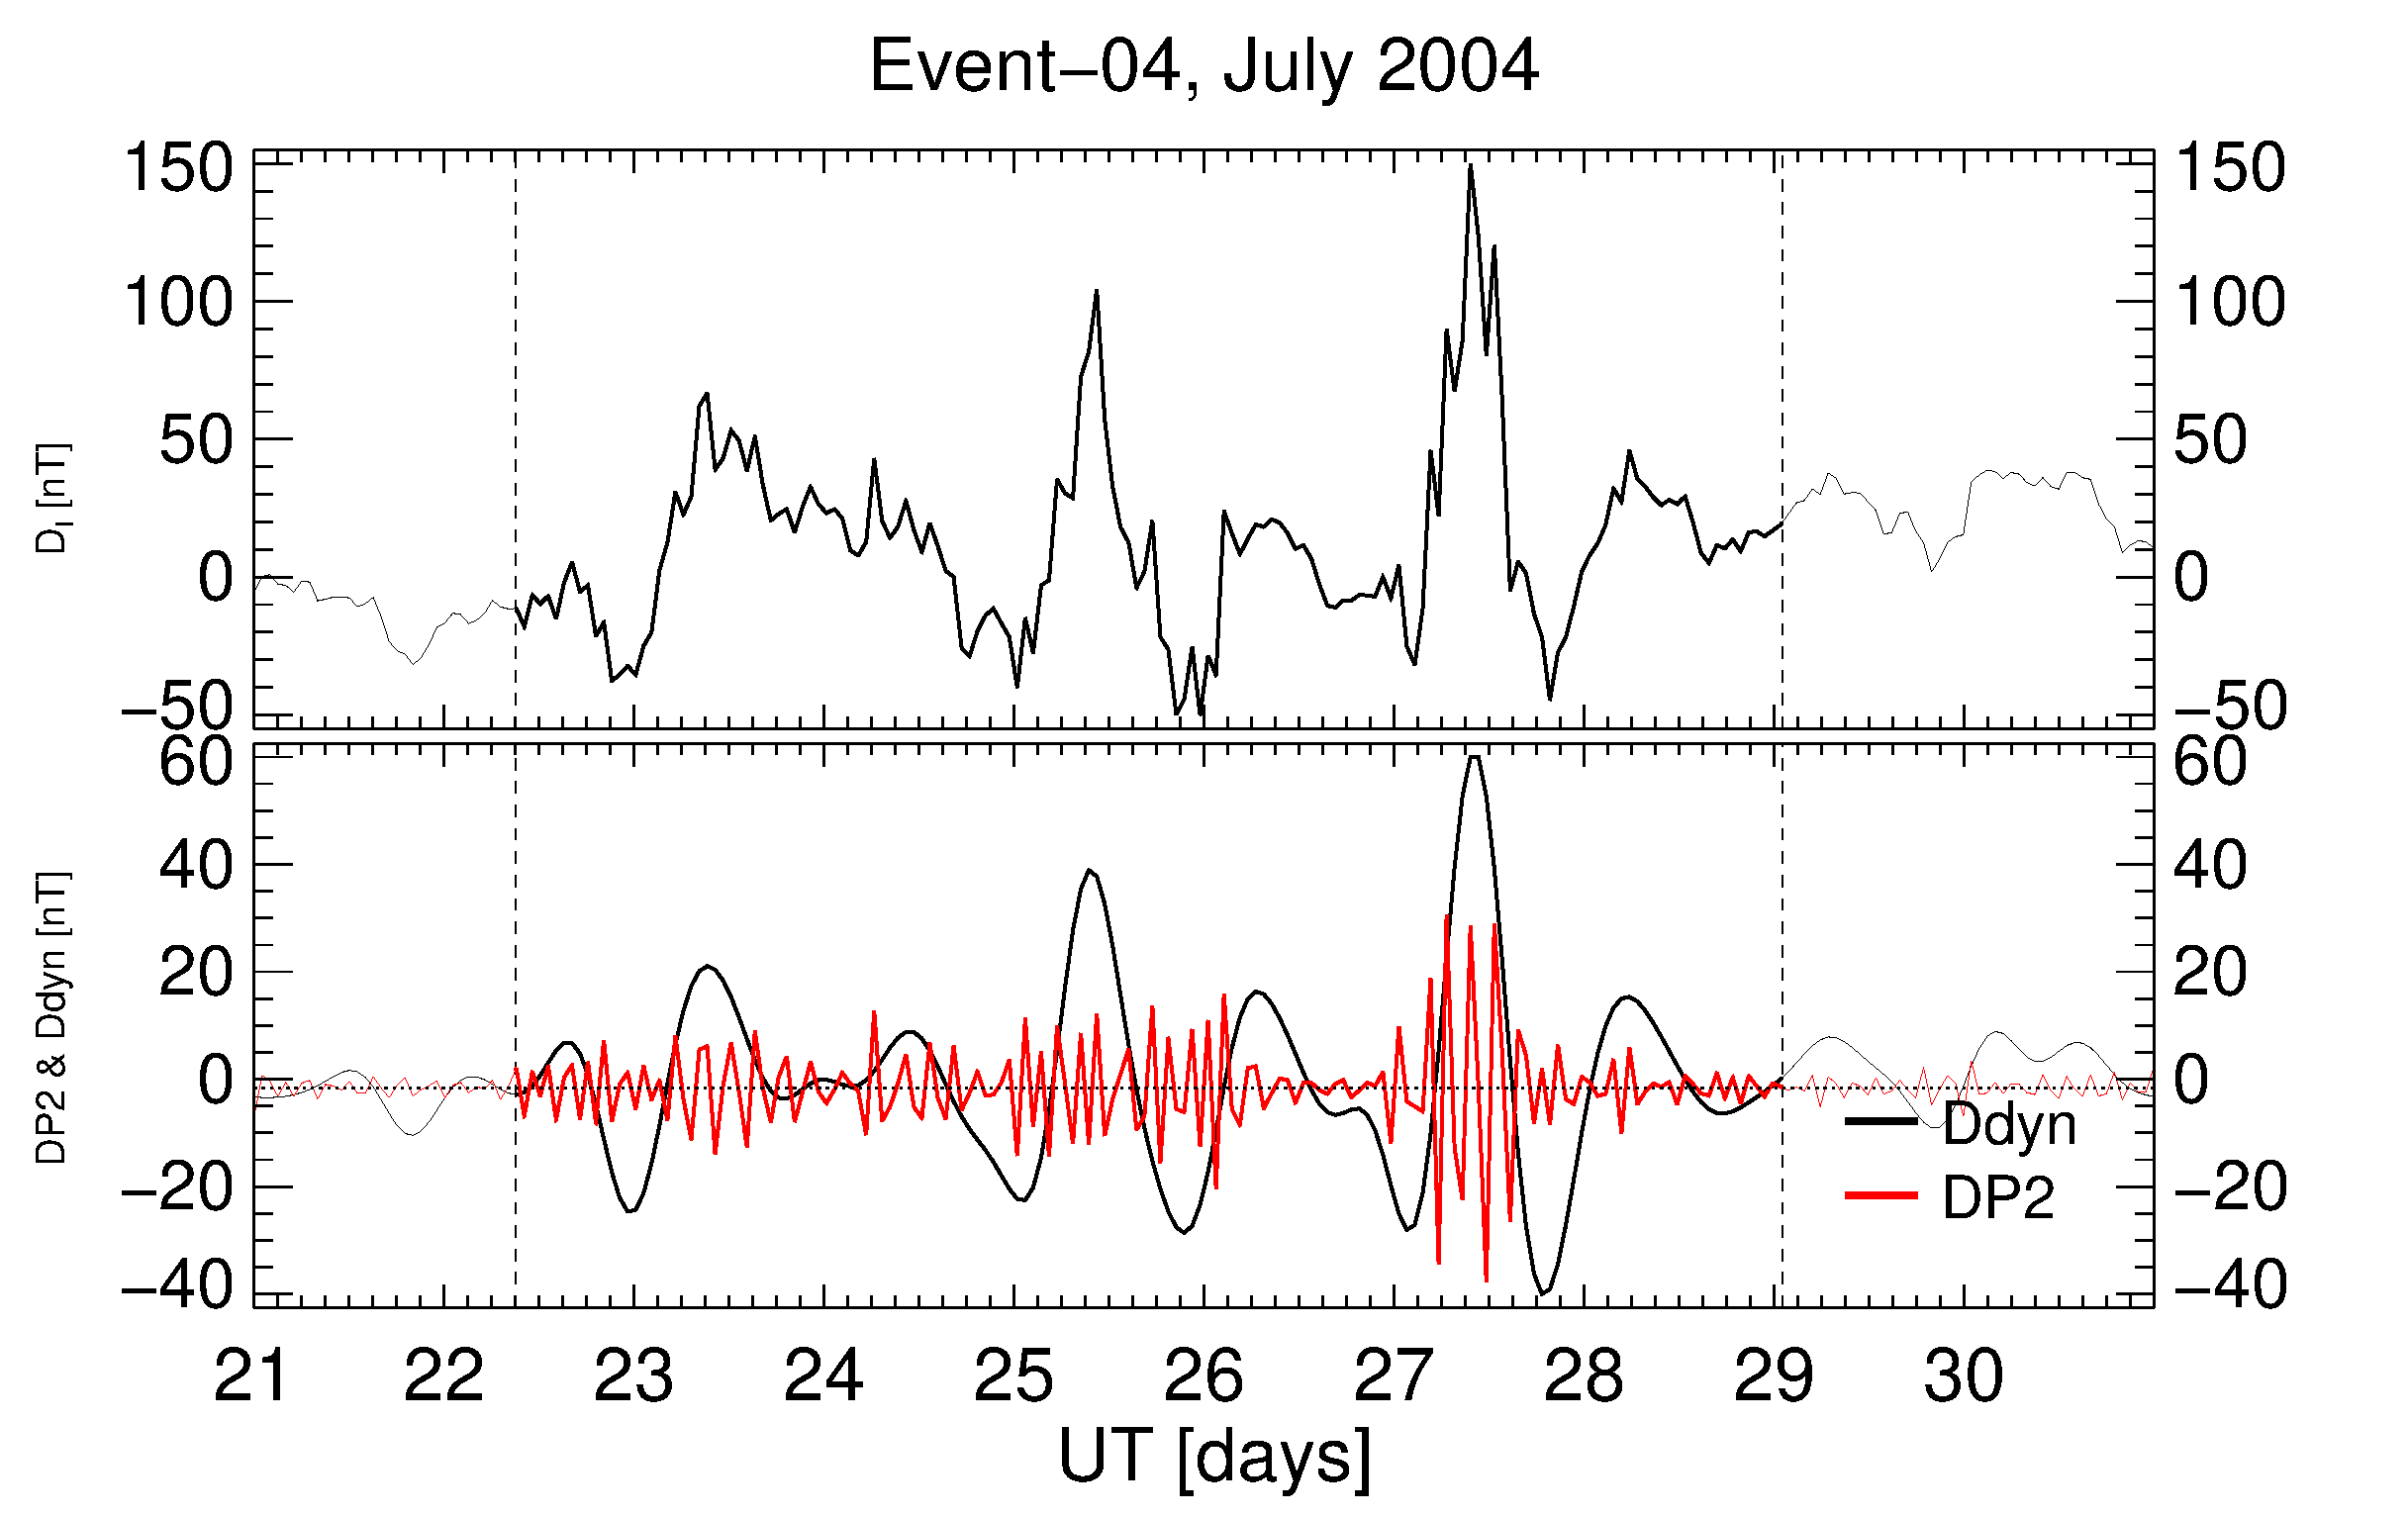
\includegraphics[width=6.0cm]{images/diono/iono_PI_V1_2004-07-21.eps}
     \centerline{\Large \bf   
      \hspace{0.275\textwidth}  \color{black}{}
       \hspace{0.295\textwidth}  \color{black}{}
         \hfill}
      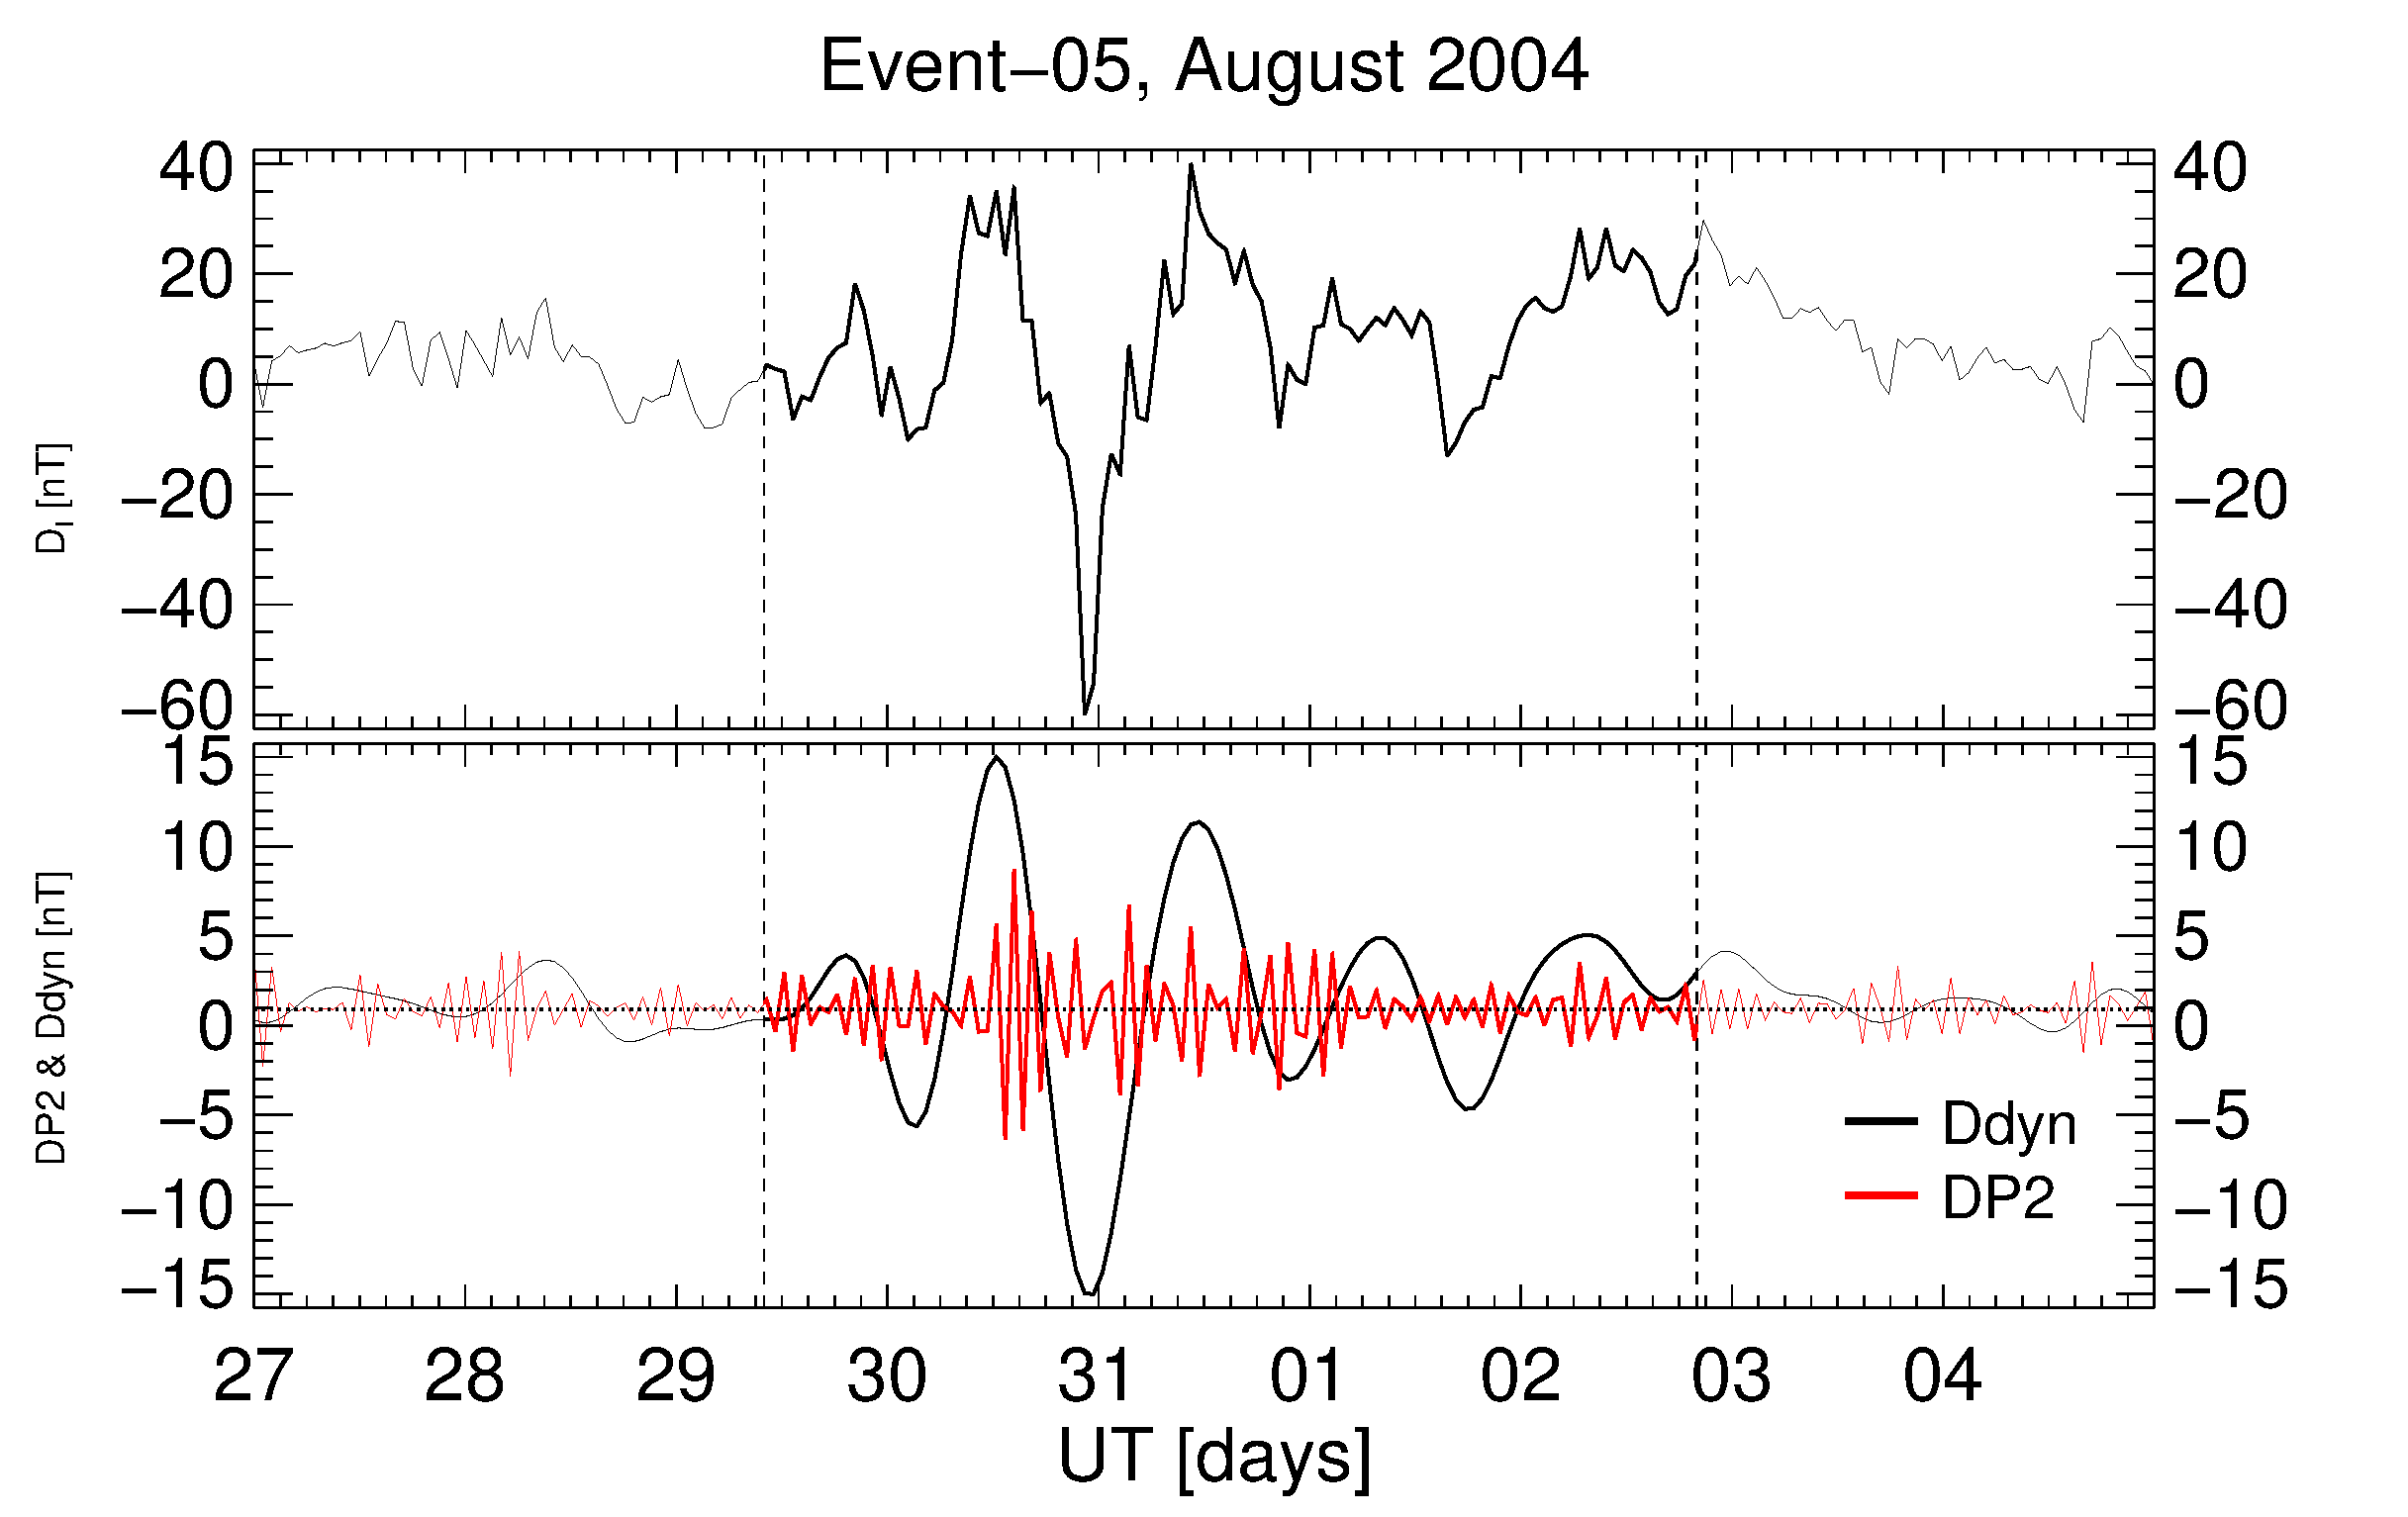
\includegraphics[width=6.0cm]{images/diono/iono_PI_V1_2004-08-27.eps}     
      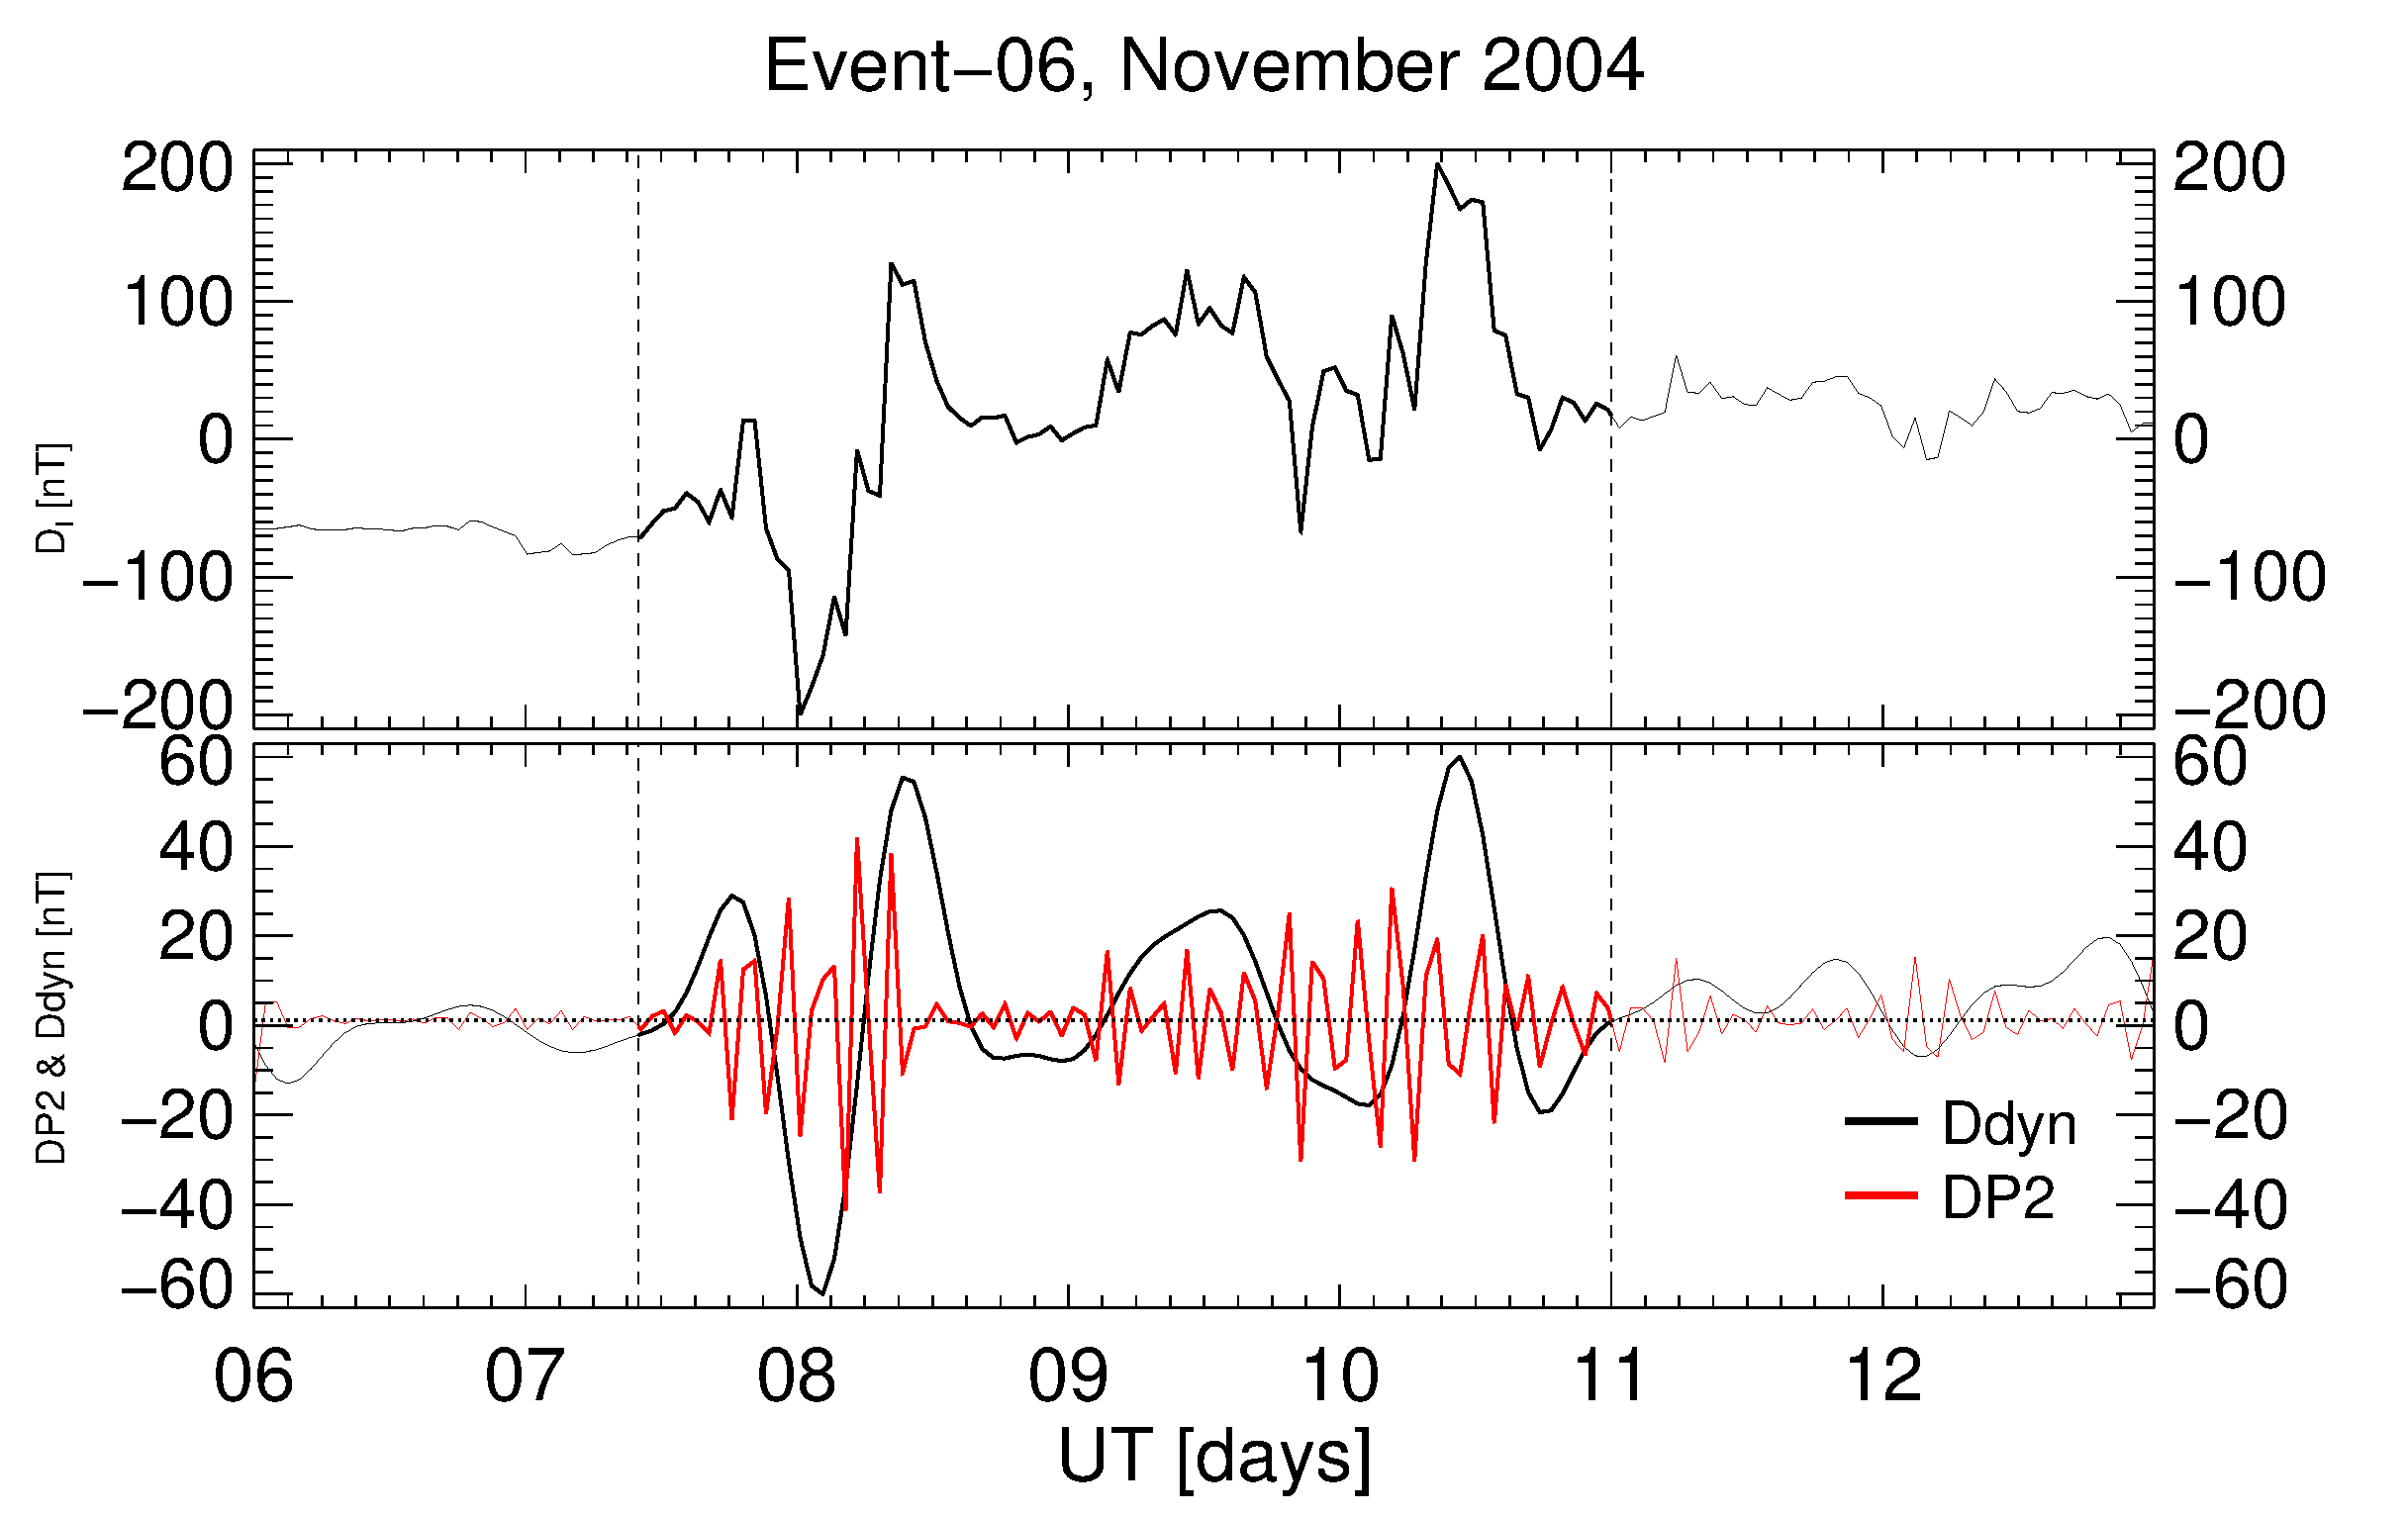
\includegraphics[width=6.0cm]{images/diono/iono_PI_V1_2004-11-06.eps}
       \centerline{\Large \bf   
      \hspace{0.275\textwidth}  \color{black}{}
       \hspace{0.295\textwidth}  \color{black}{}
         \hfill}
       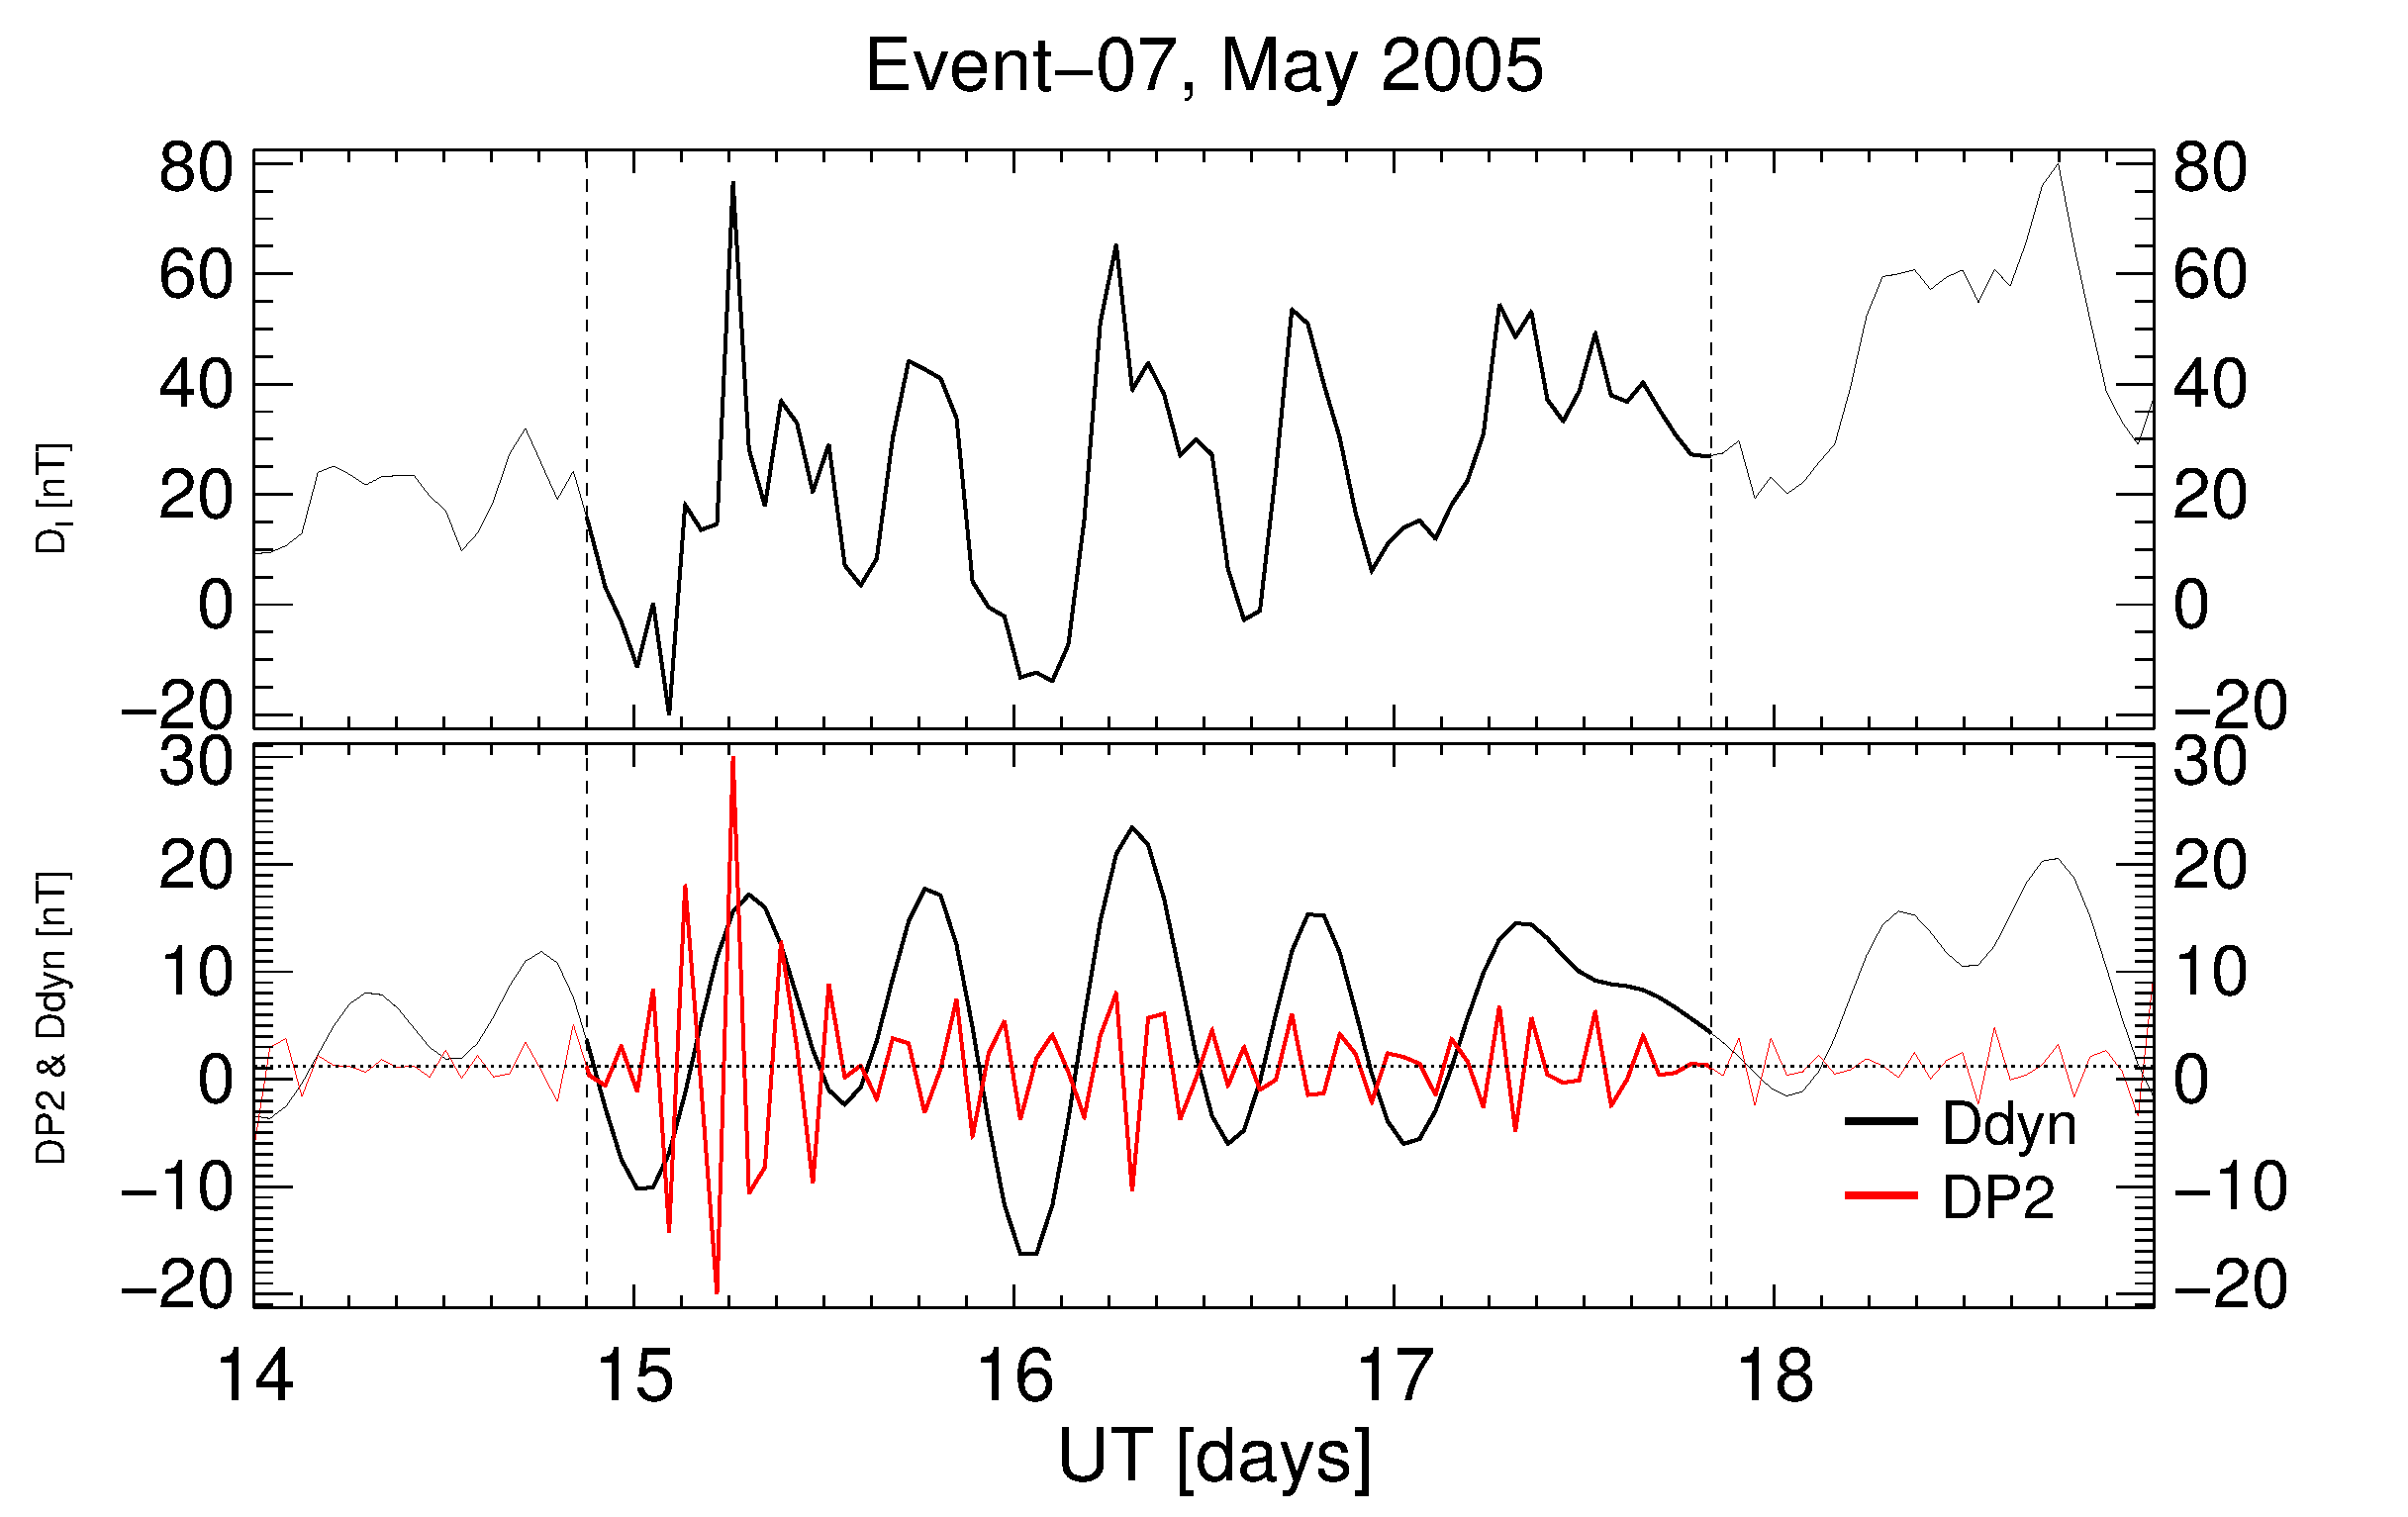
\includegraphics[width=6.0cm]{images/diono/iono_PI_V1_2005-05-14.eps}     
       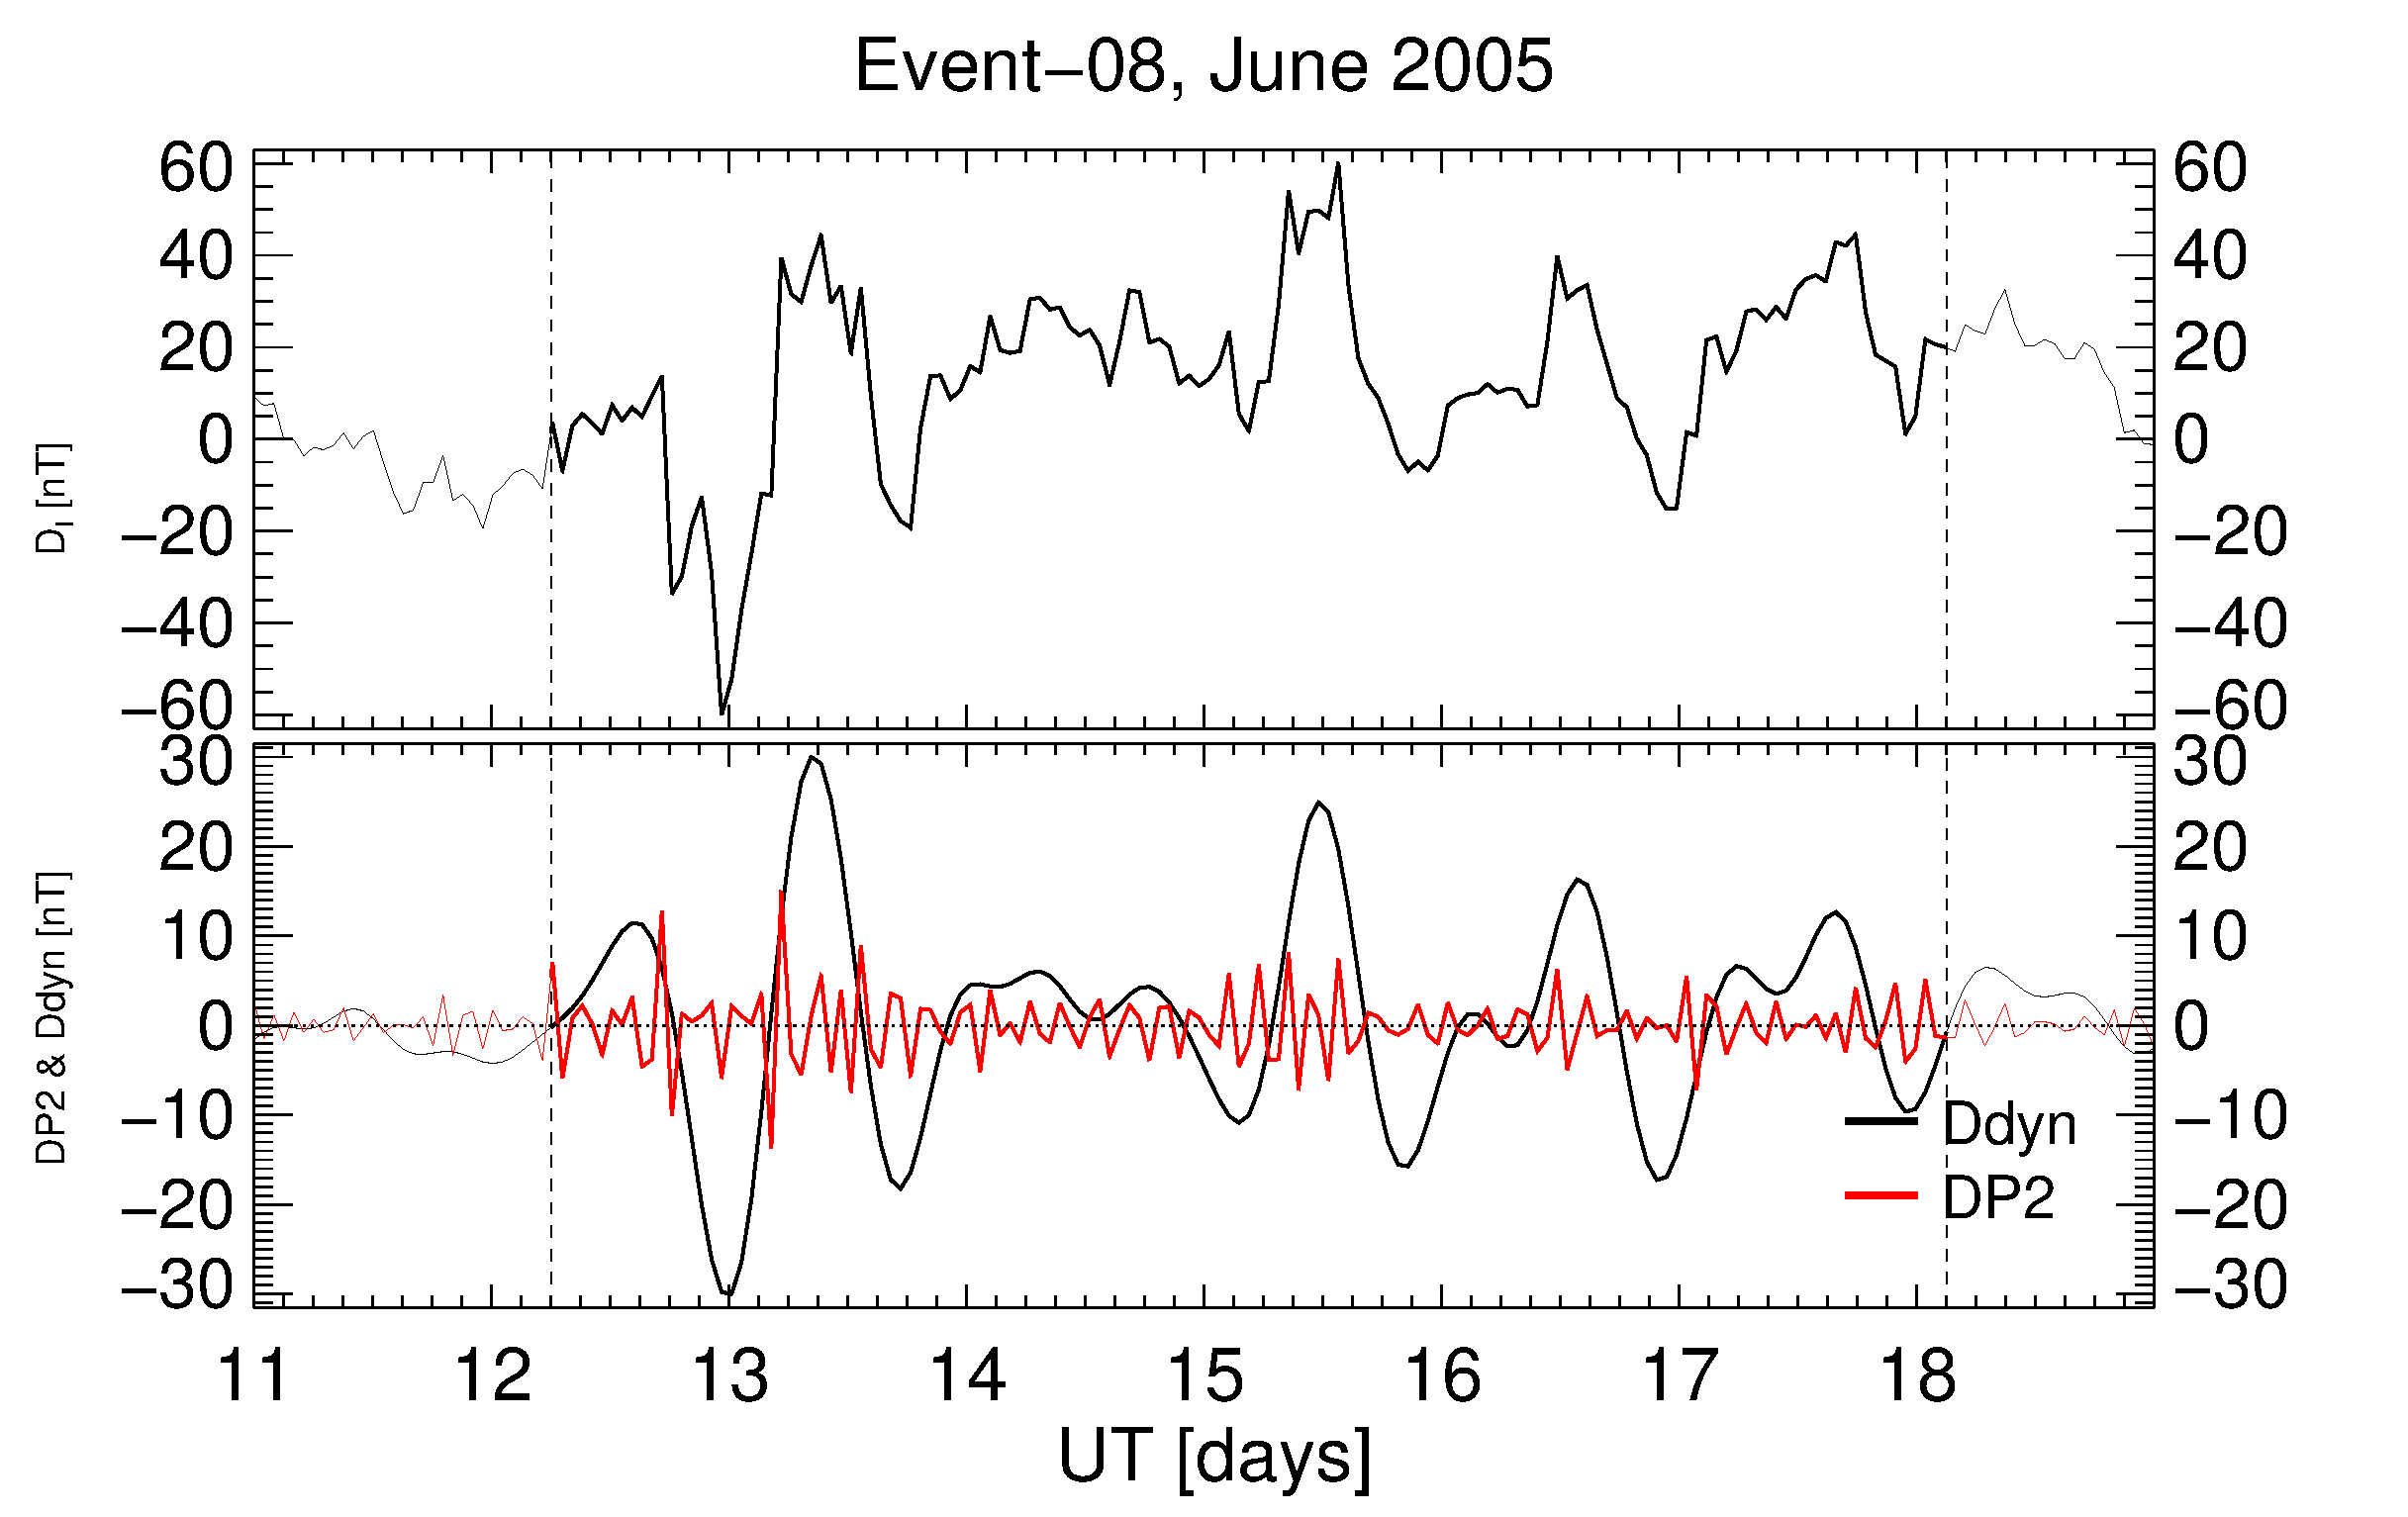
\includegraphics[width=6.0cm]{images/diono/iono_PI_V1_2005-06-11.eps}

       \centerline{\Large \bf   
      \hspace{0.275\textwidth}  \color{black}{}
       \hspace{0.295\textwidth}  \color{black}{}
         \hfill}
       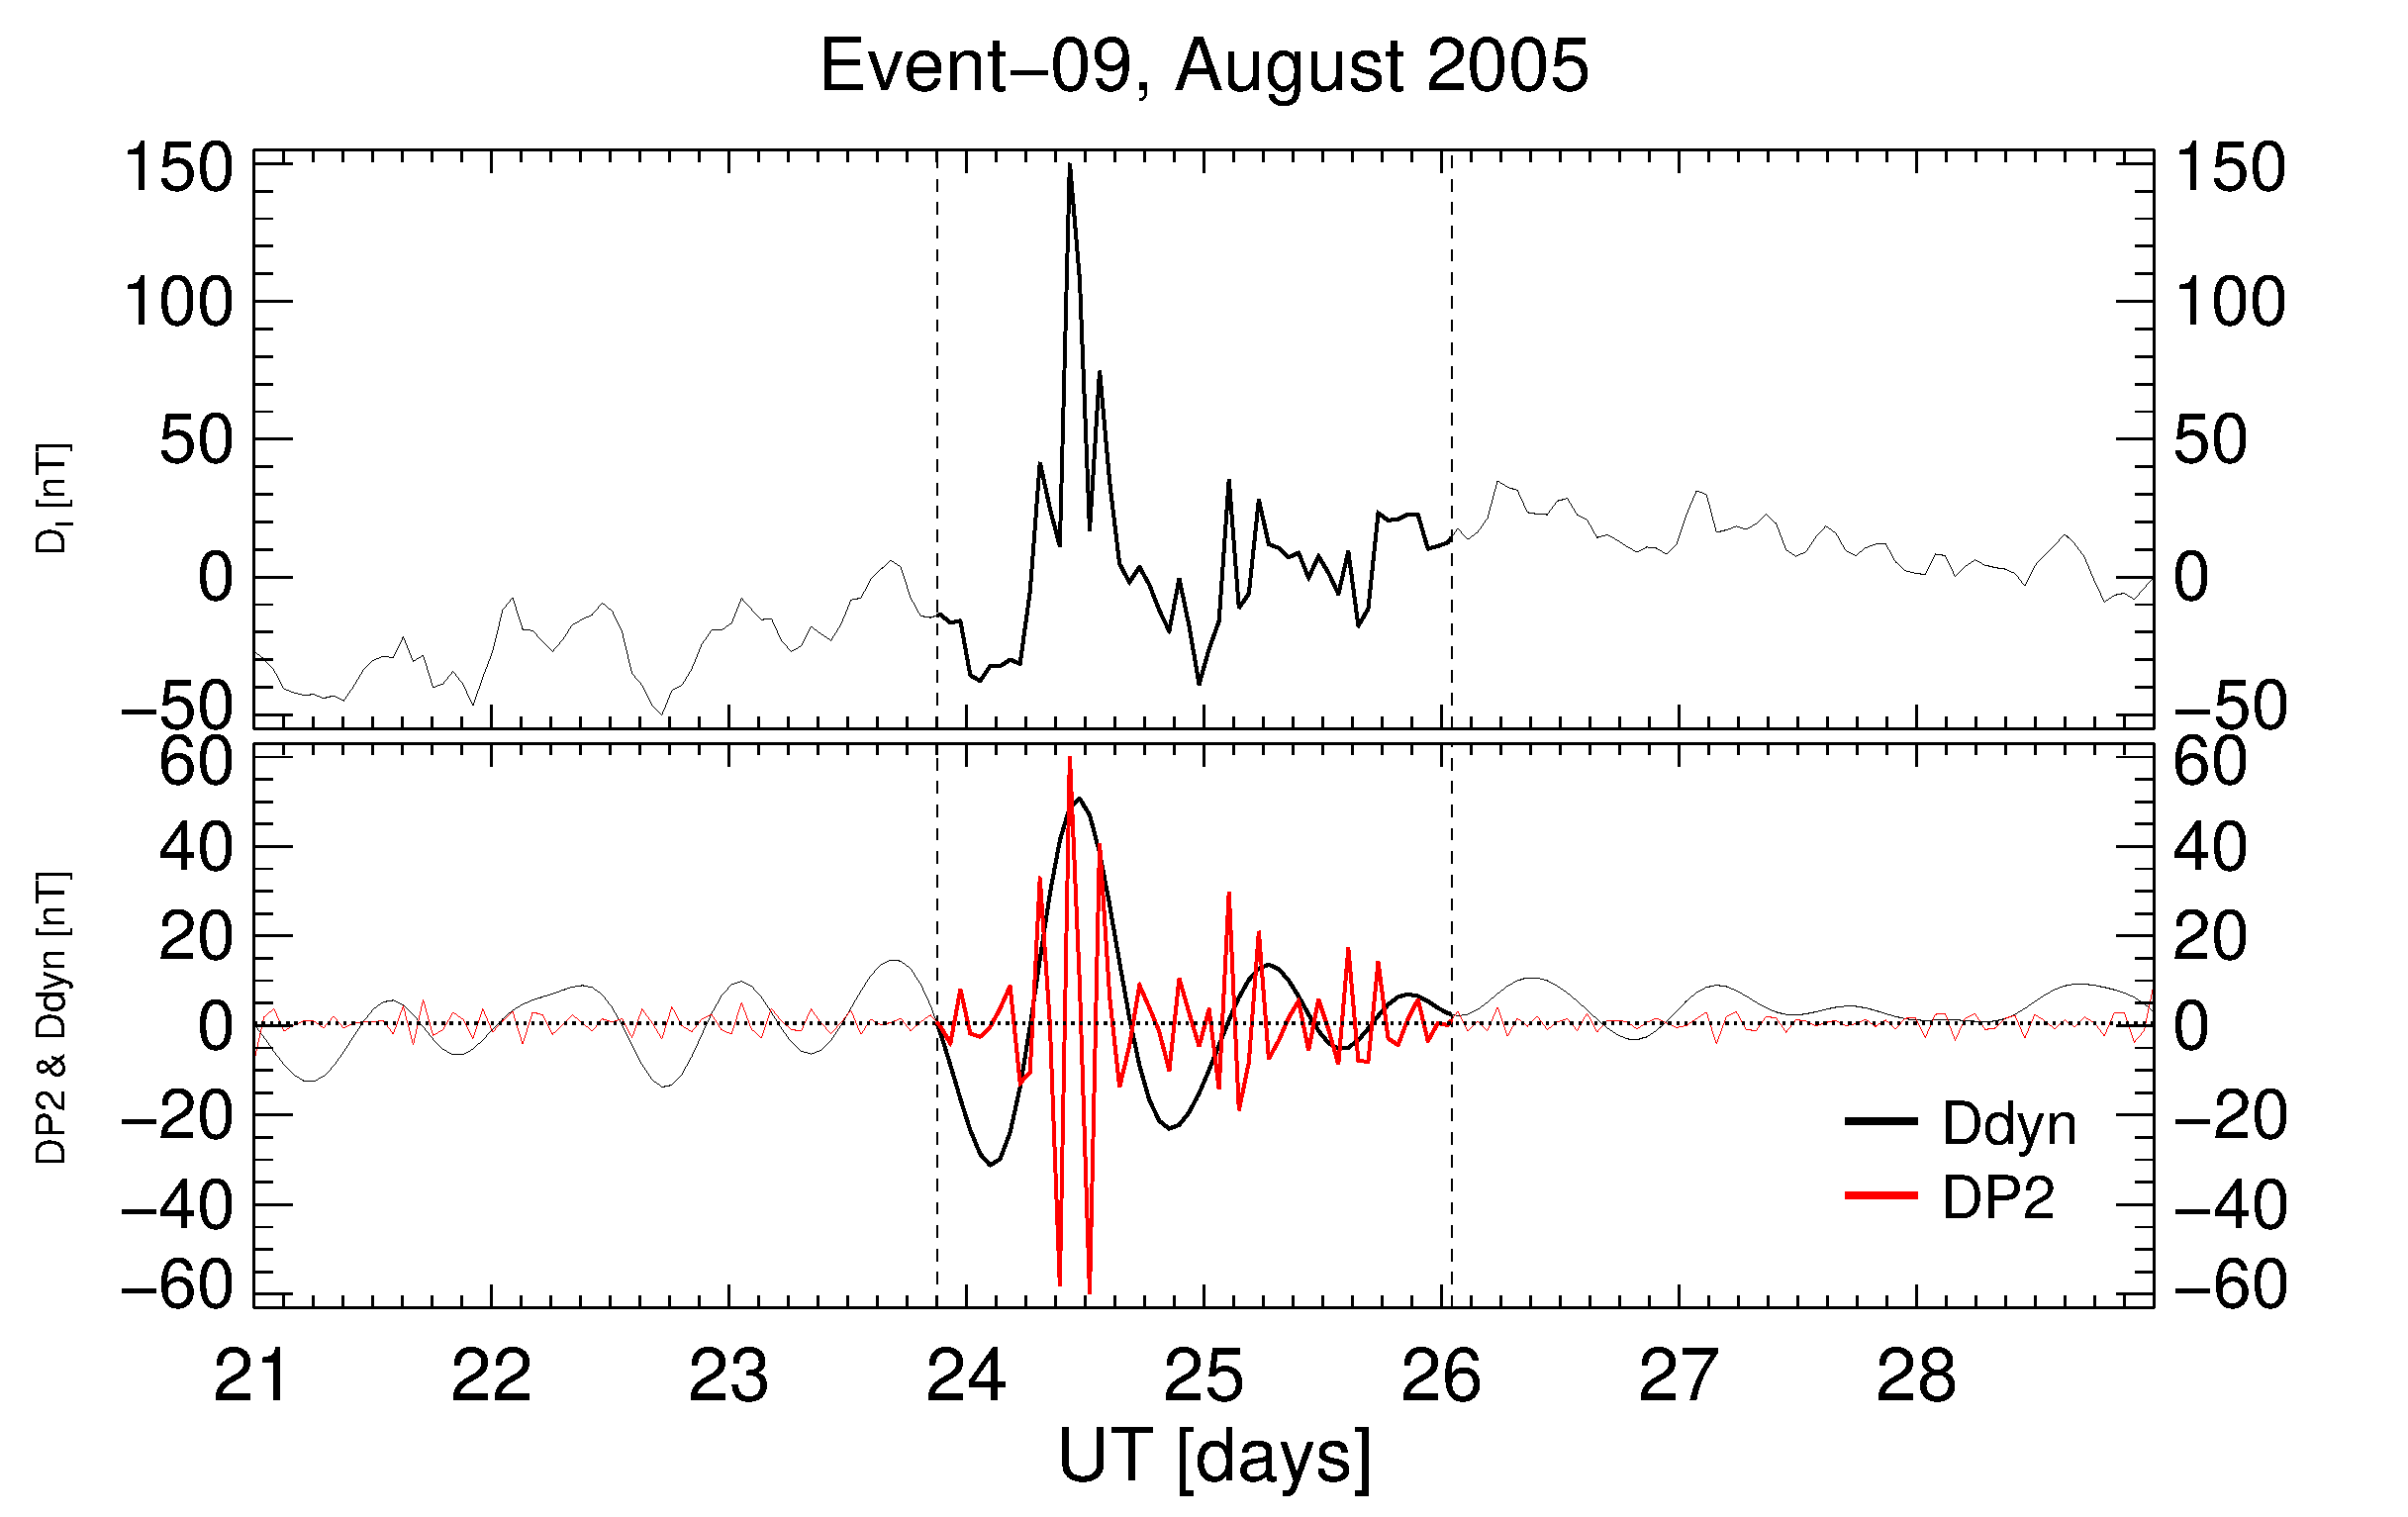
\includegraphics[width=6.0cm]{images/diono/iono_PI_V1_2005-08-21.eps}     
       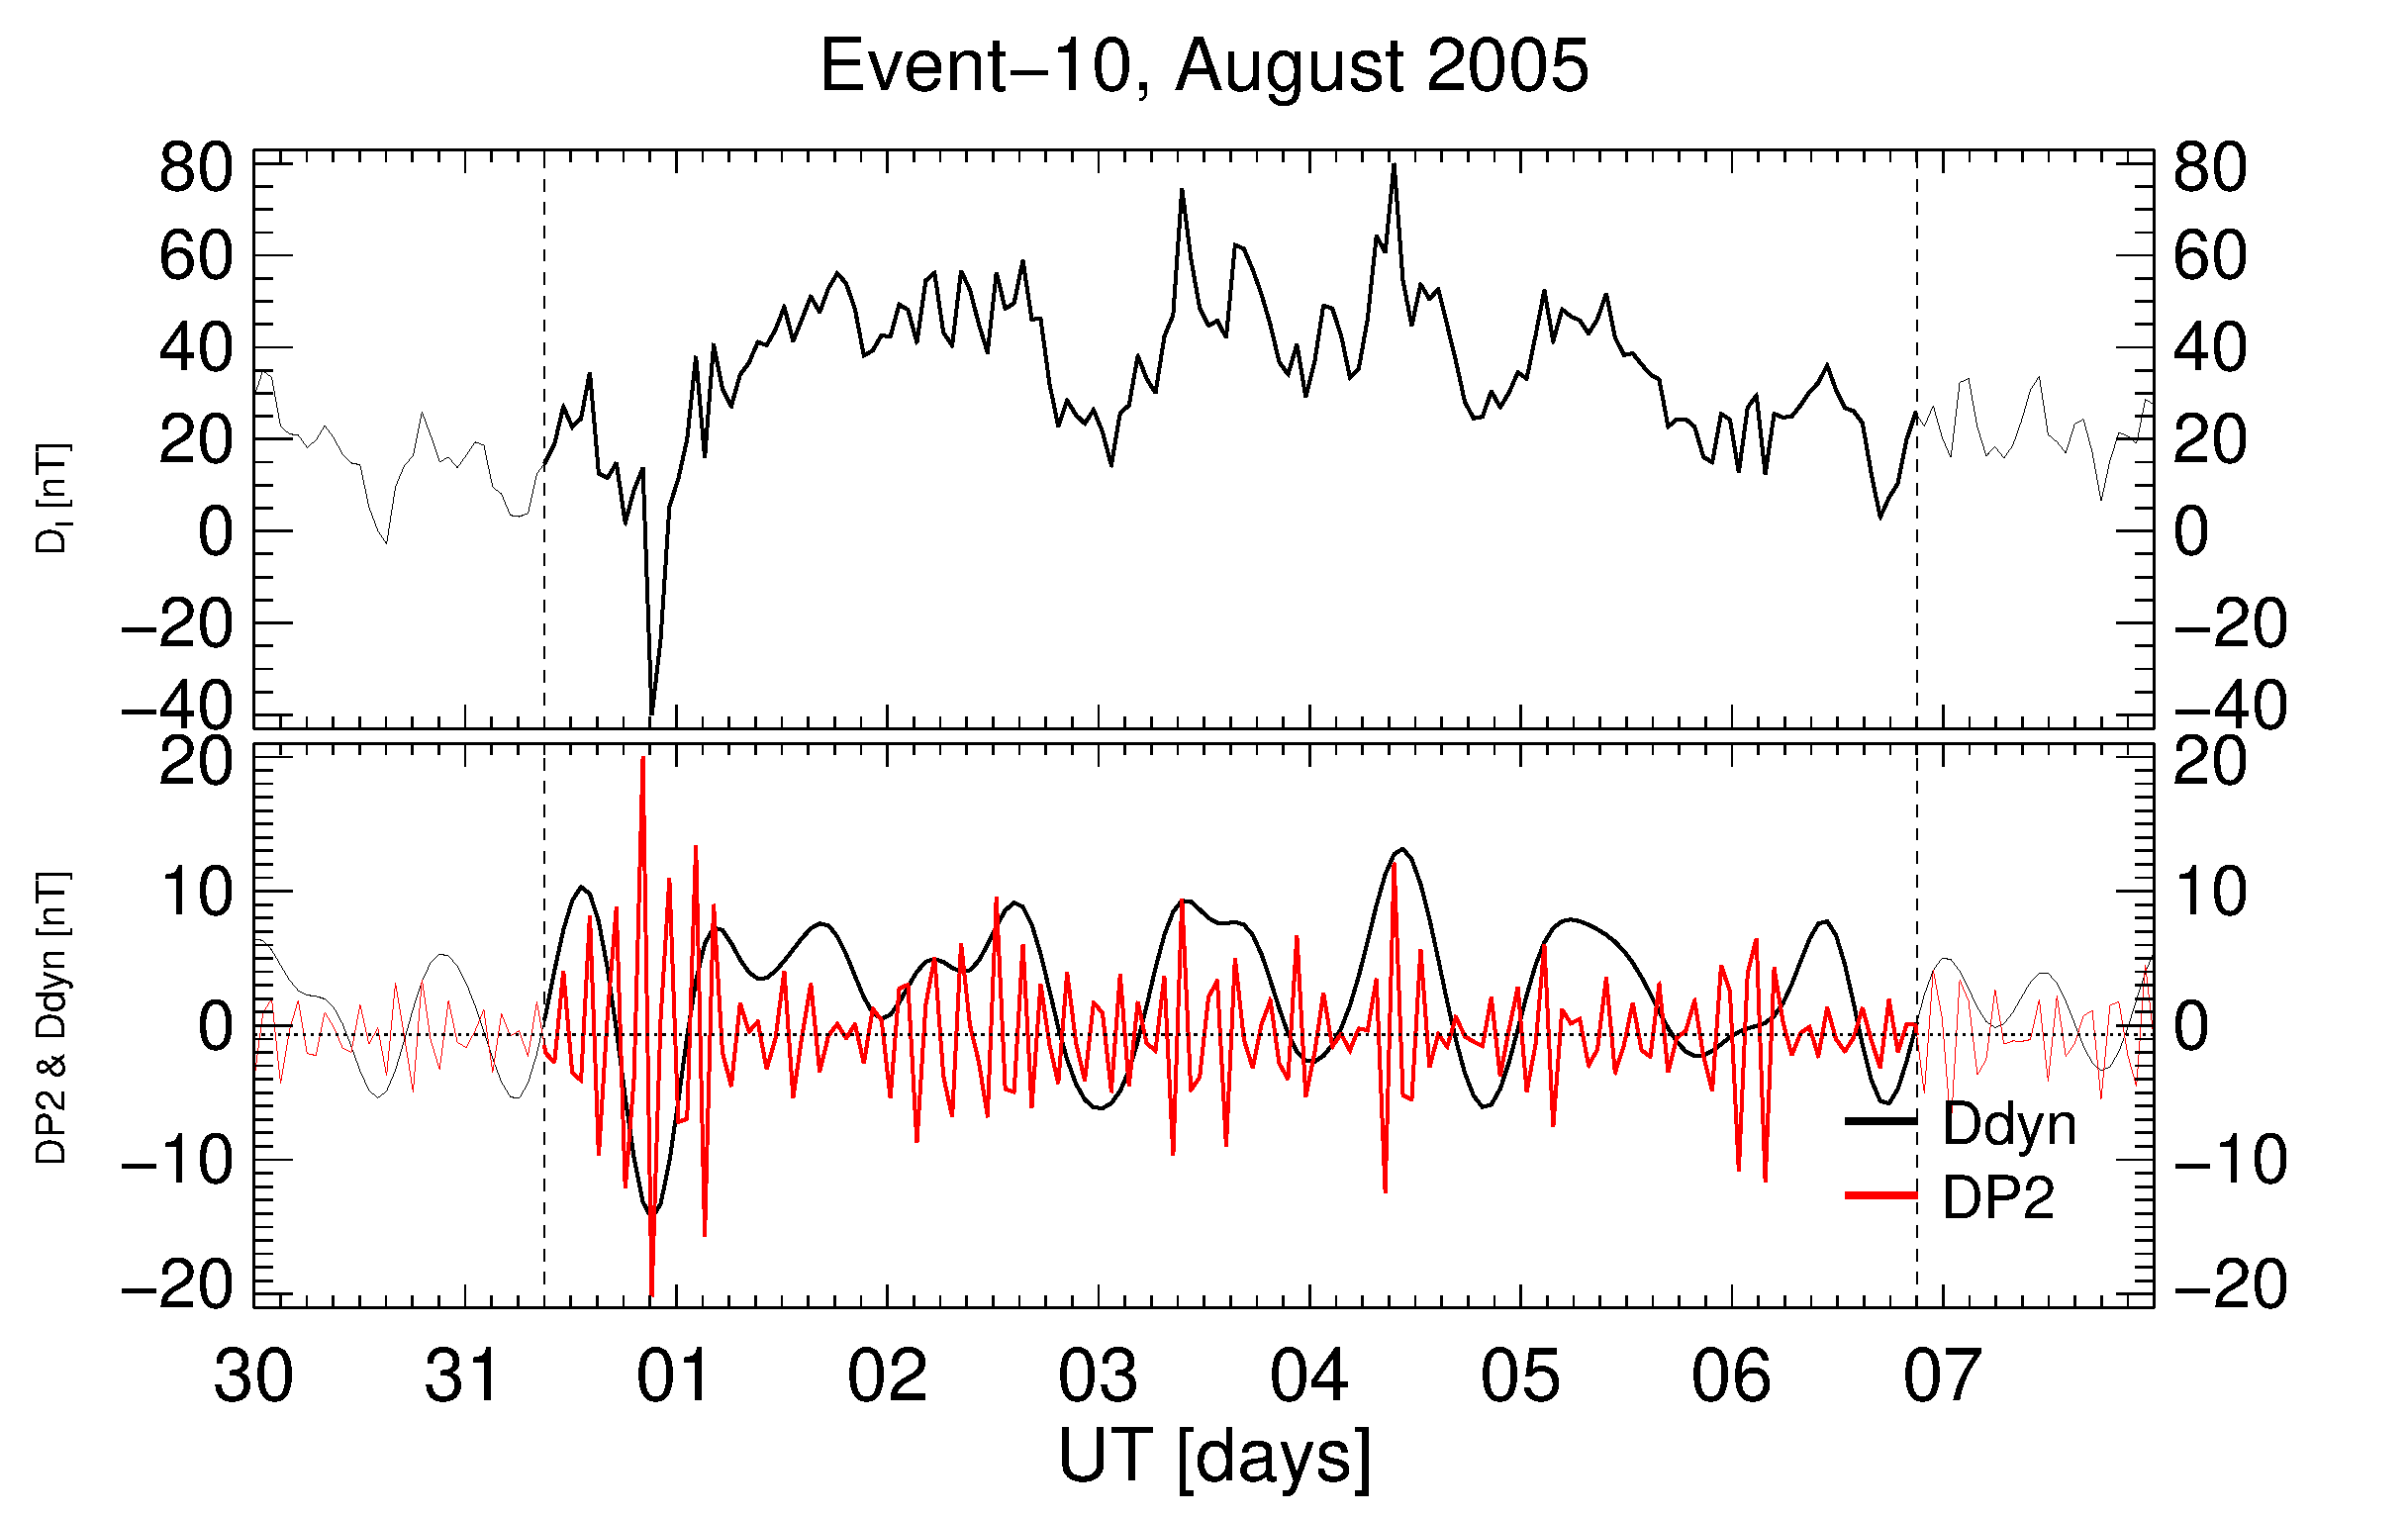
\includegraphics[width=6.0cm]{images/diono/iono_PI_V1_2005-08-30.eps}
       
       \caption{Ionospheric Magnetic Disturbance contribution (top panels) and the isolated Ddyn and DP2 geomagnetic contribution (bottom panels).}
    \label{fig:iono_resp2}
\end{figure*}


\begin{figure*}[h!]
    \centering
    \centerline{\Large \bf   
      %\hspace{0.18\textwidth}  \color{black}{\Large{Res}}
       %\hspace{0.28\textwidth}  \color{black}{\Large{Res+TC}}
         \hfill}
          \centerline{\Large \bf   
      \hspace{0.26\textwidth}  \color{black}{}
       \hspace{0.31\textwidth}  \color{black}{}
         \hfill}
     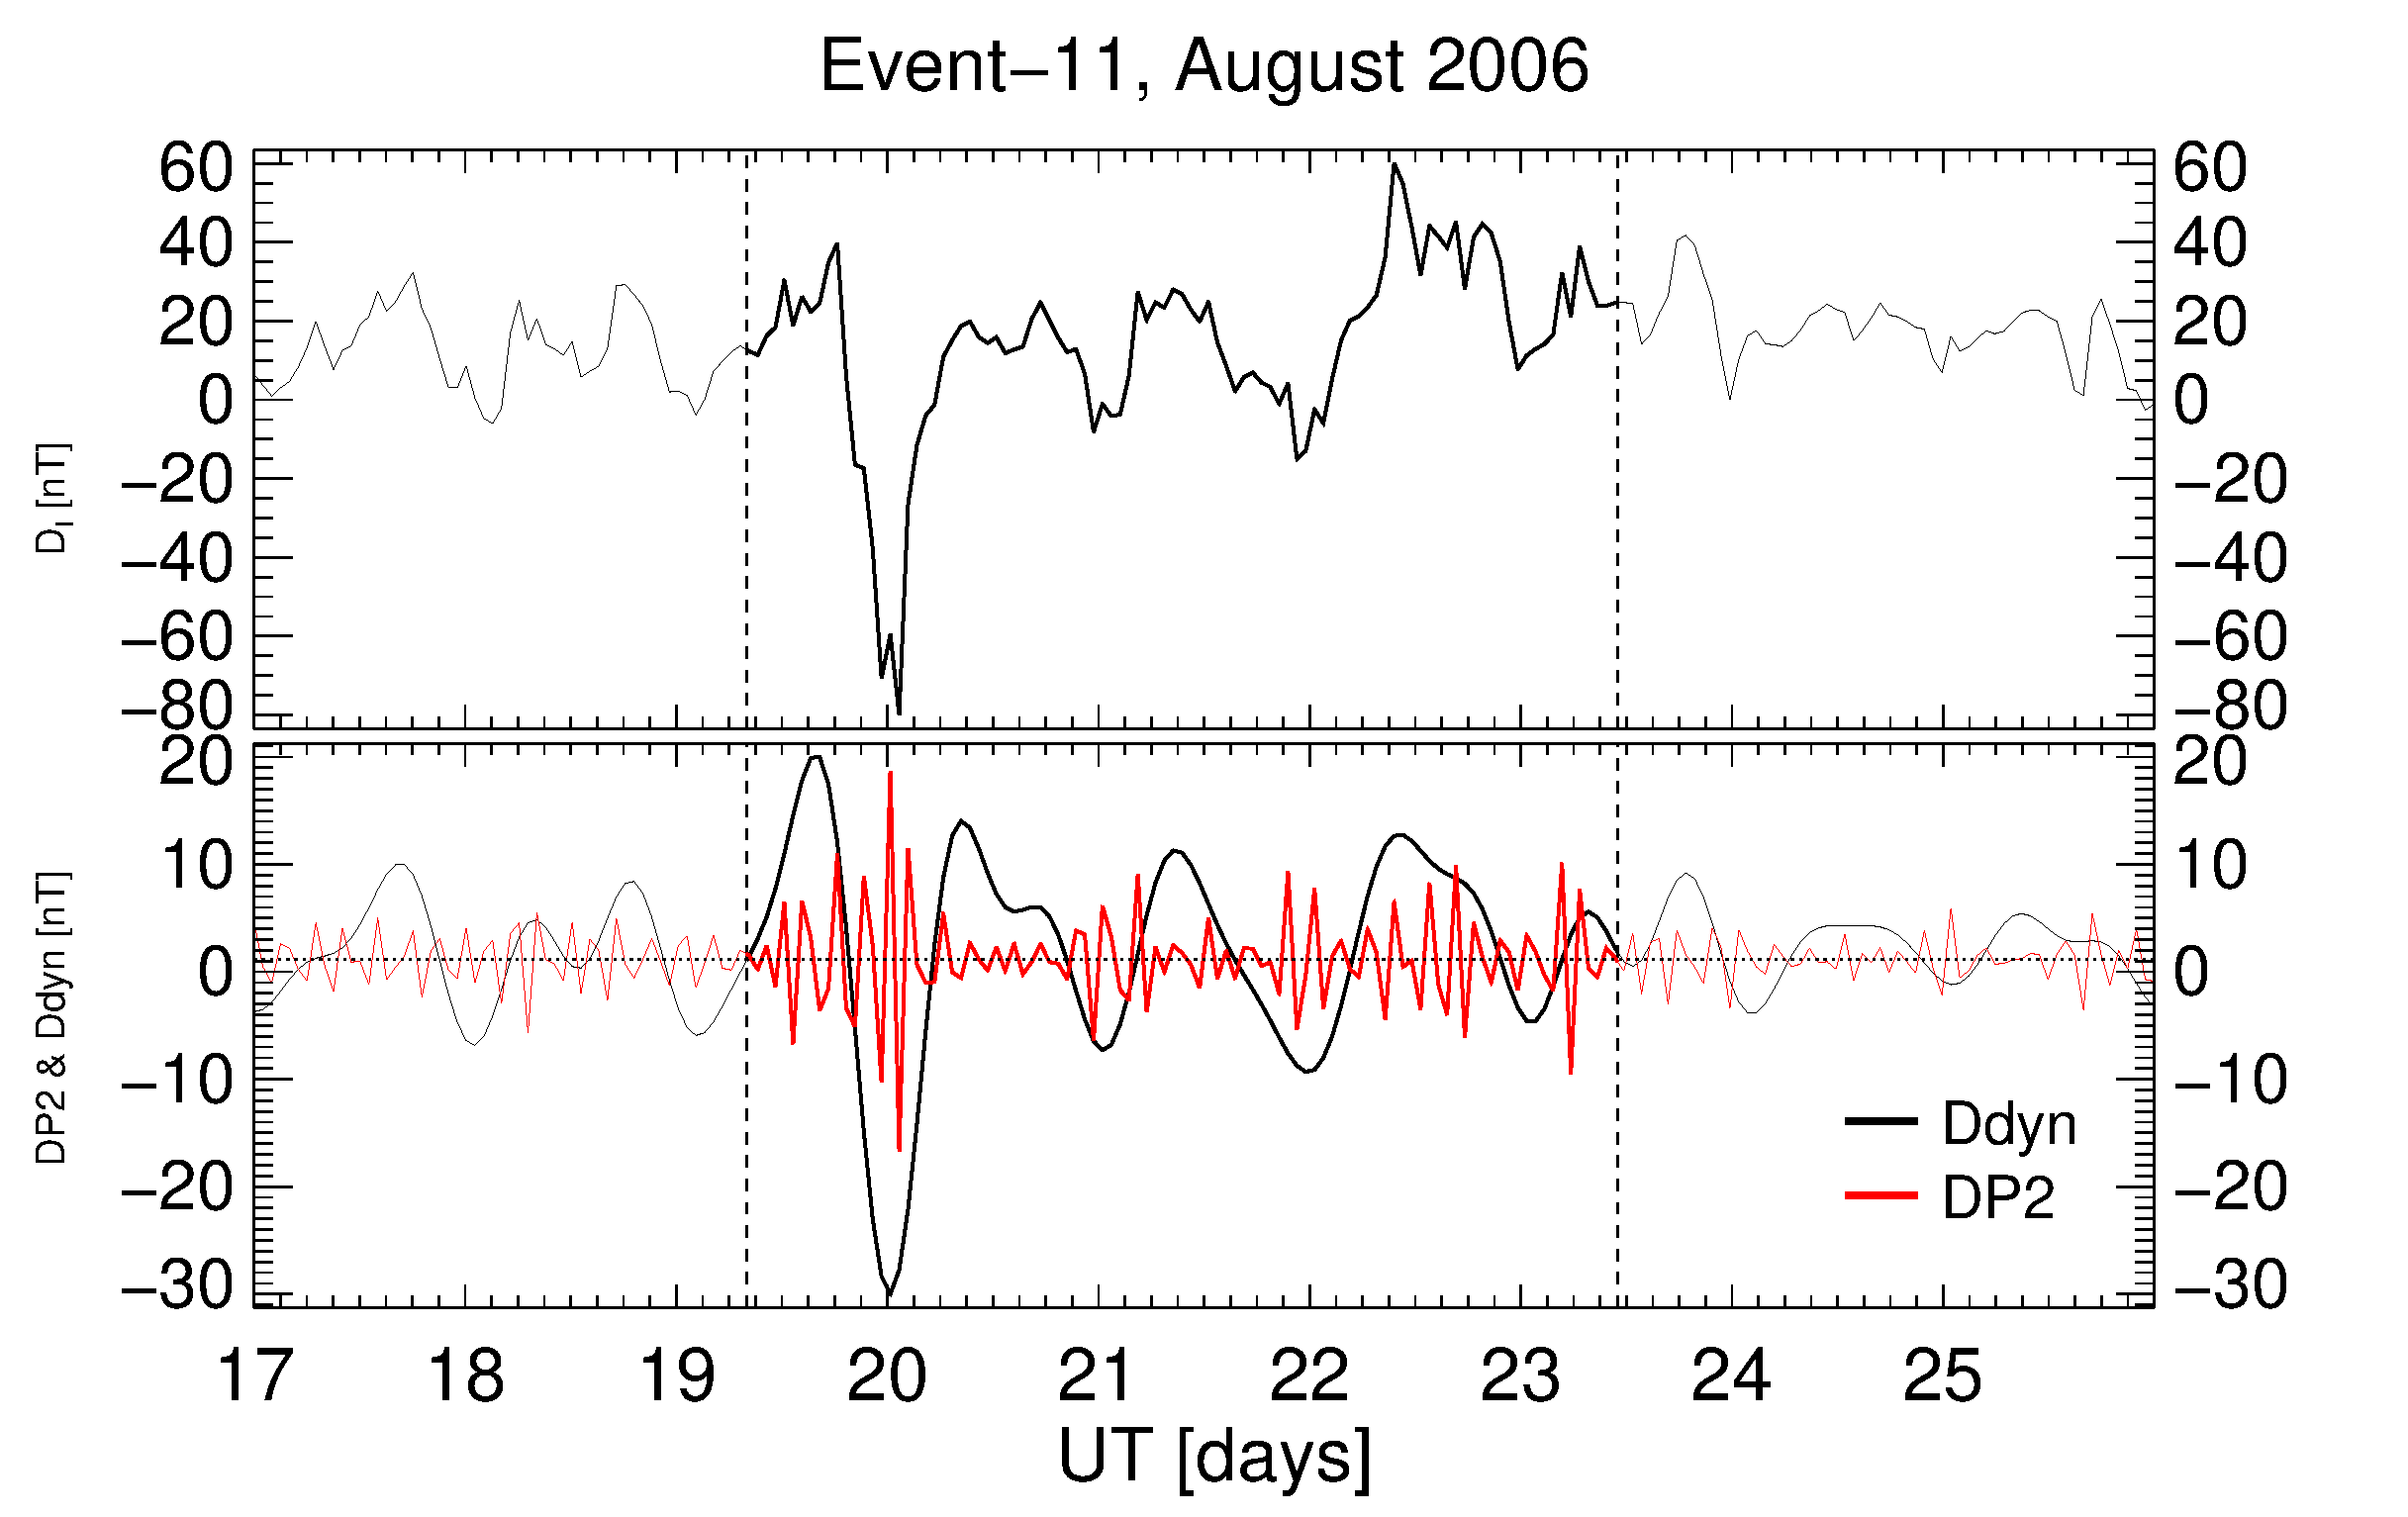
\includegraphics[width=6.0cm]{images/diono/iono_PI_V1_2006-08-17.eps}
     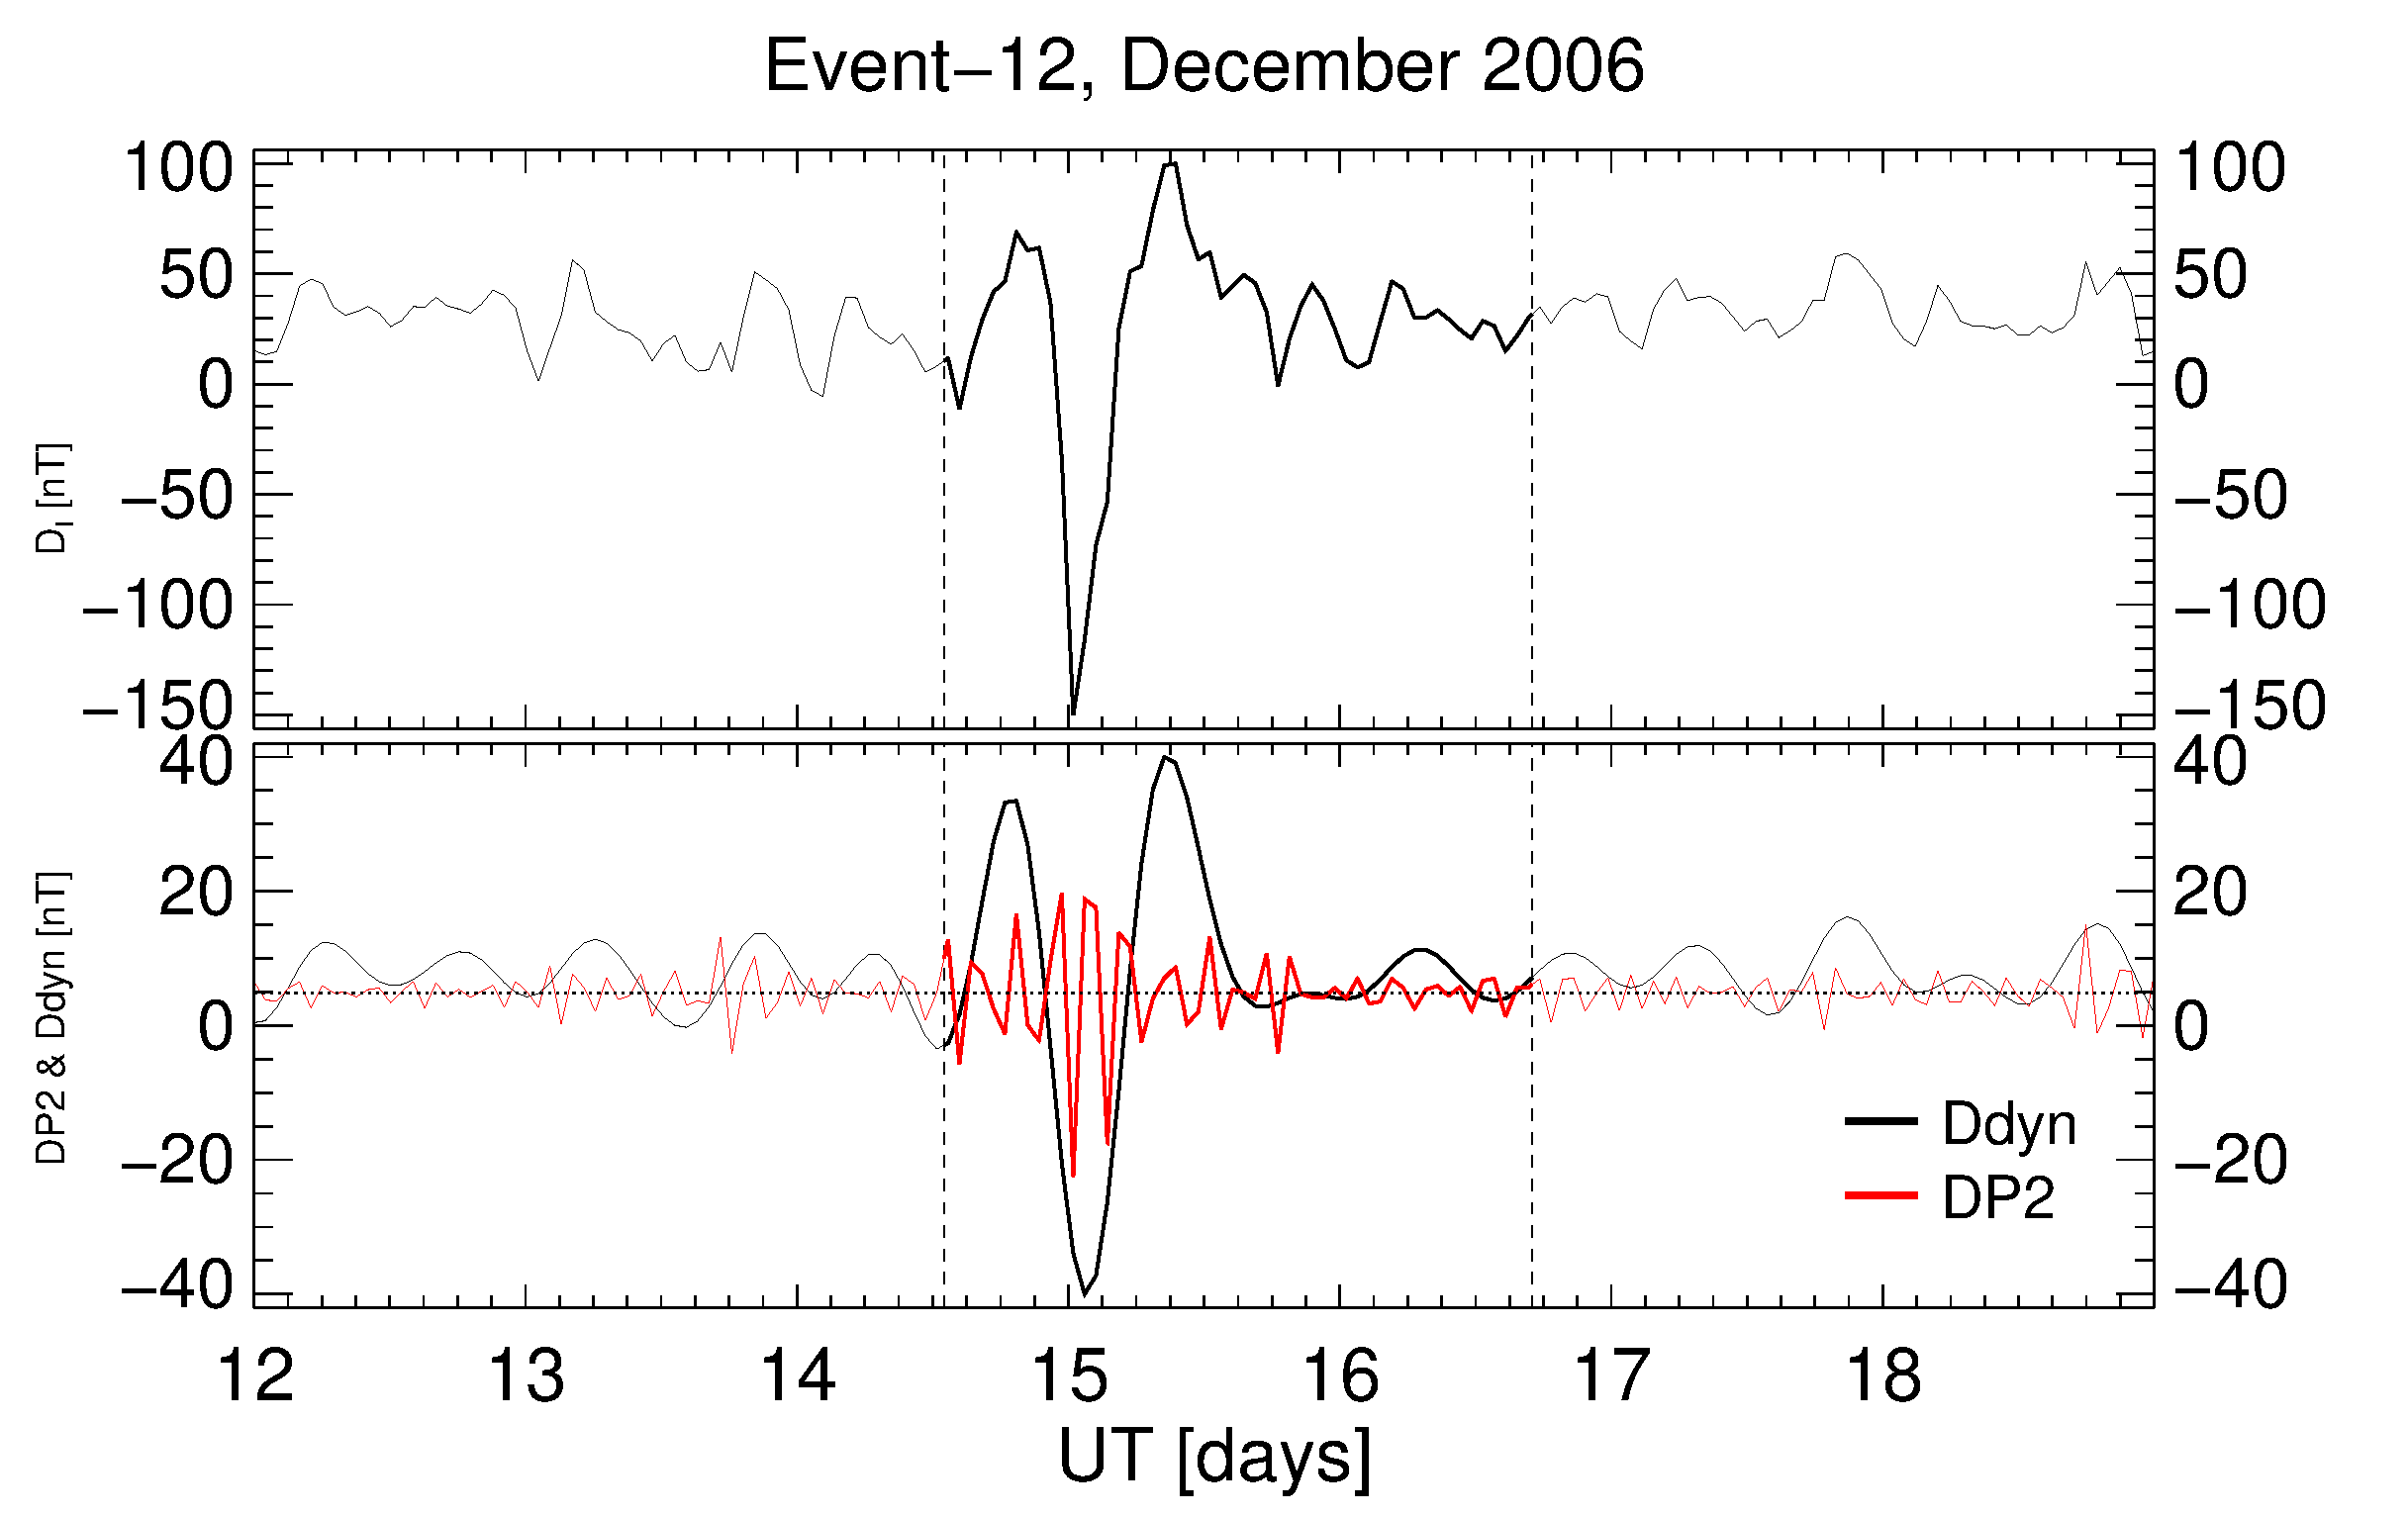
\includegraphics[width=6.0cm]{images/diono/iono_PI_V1_2006-12-12.eps}
     \centerline{\Large \bf   
      \hspace{0.275\textwidth}  \color{black}{}
       \hspace{0.295\textwidth}  \color{black}{}
         \hfill}
     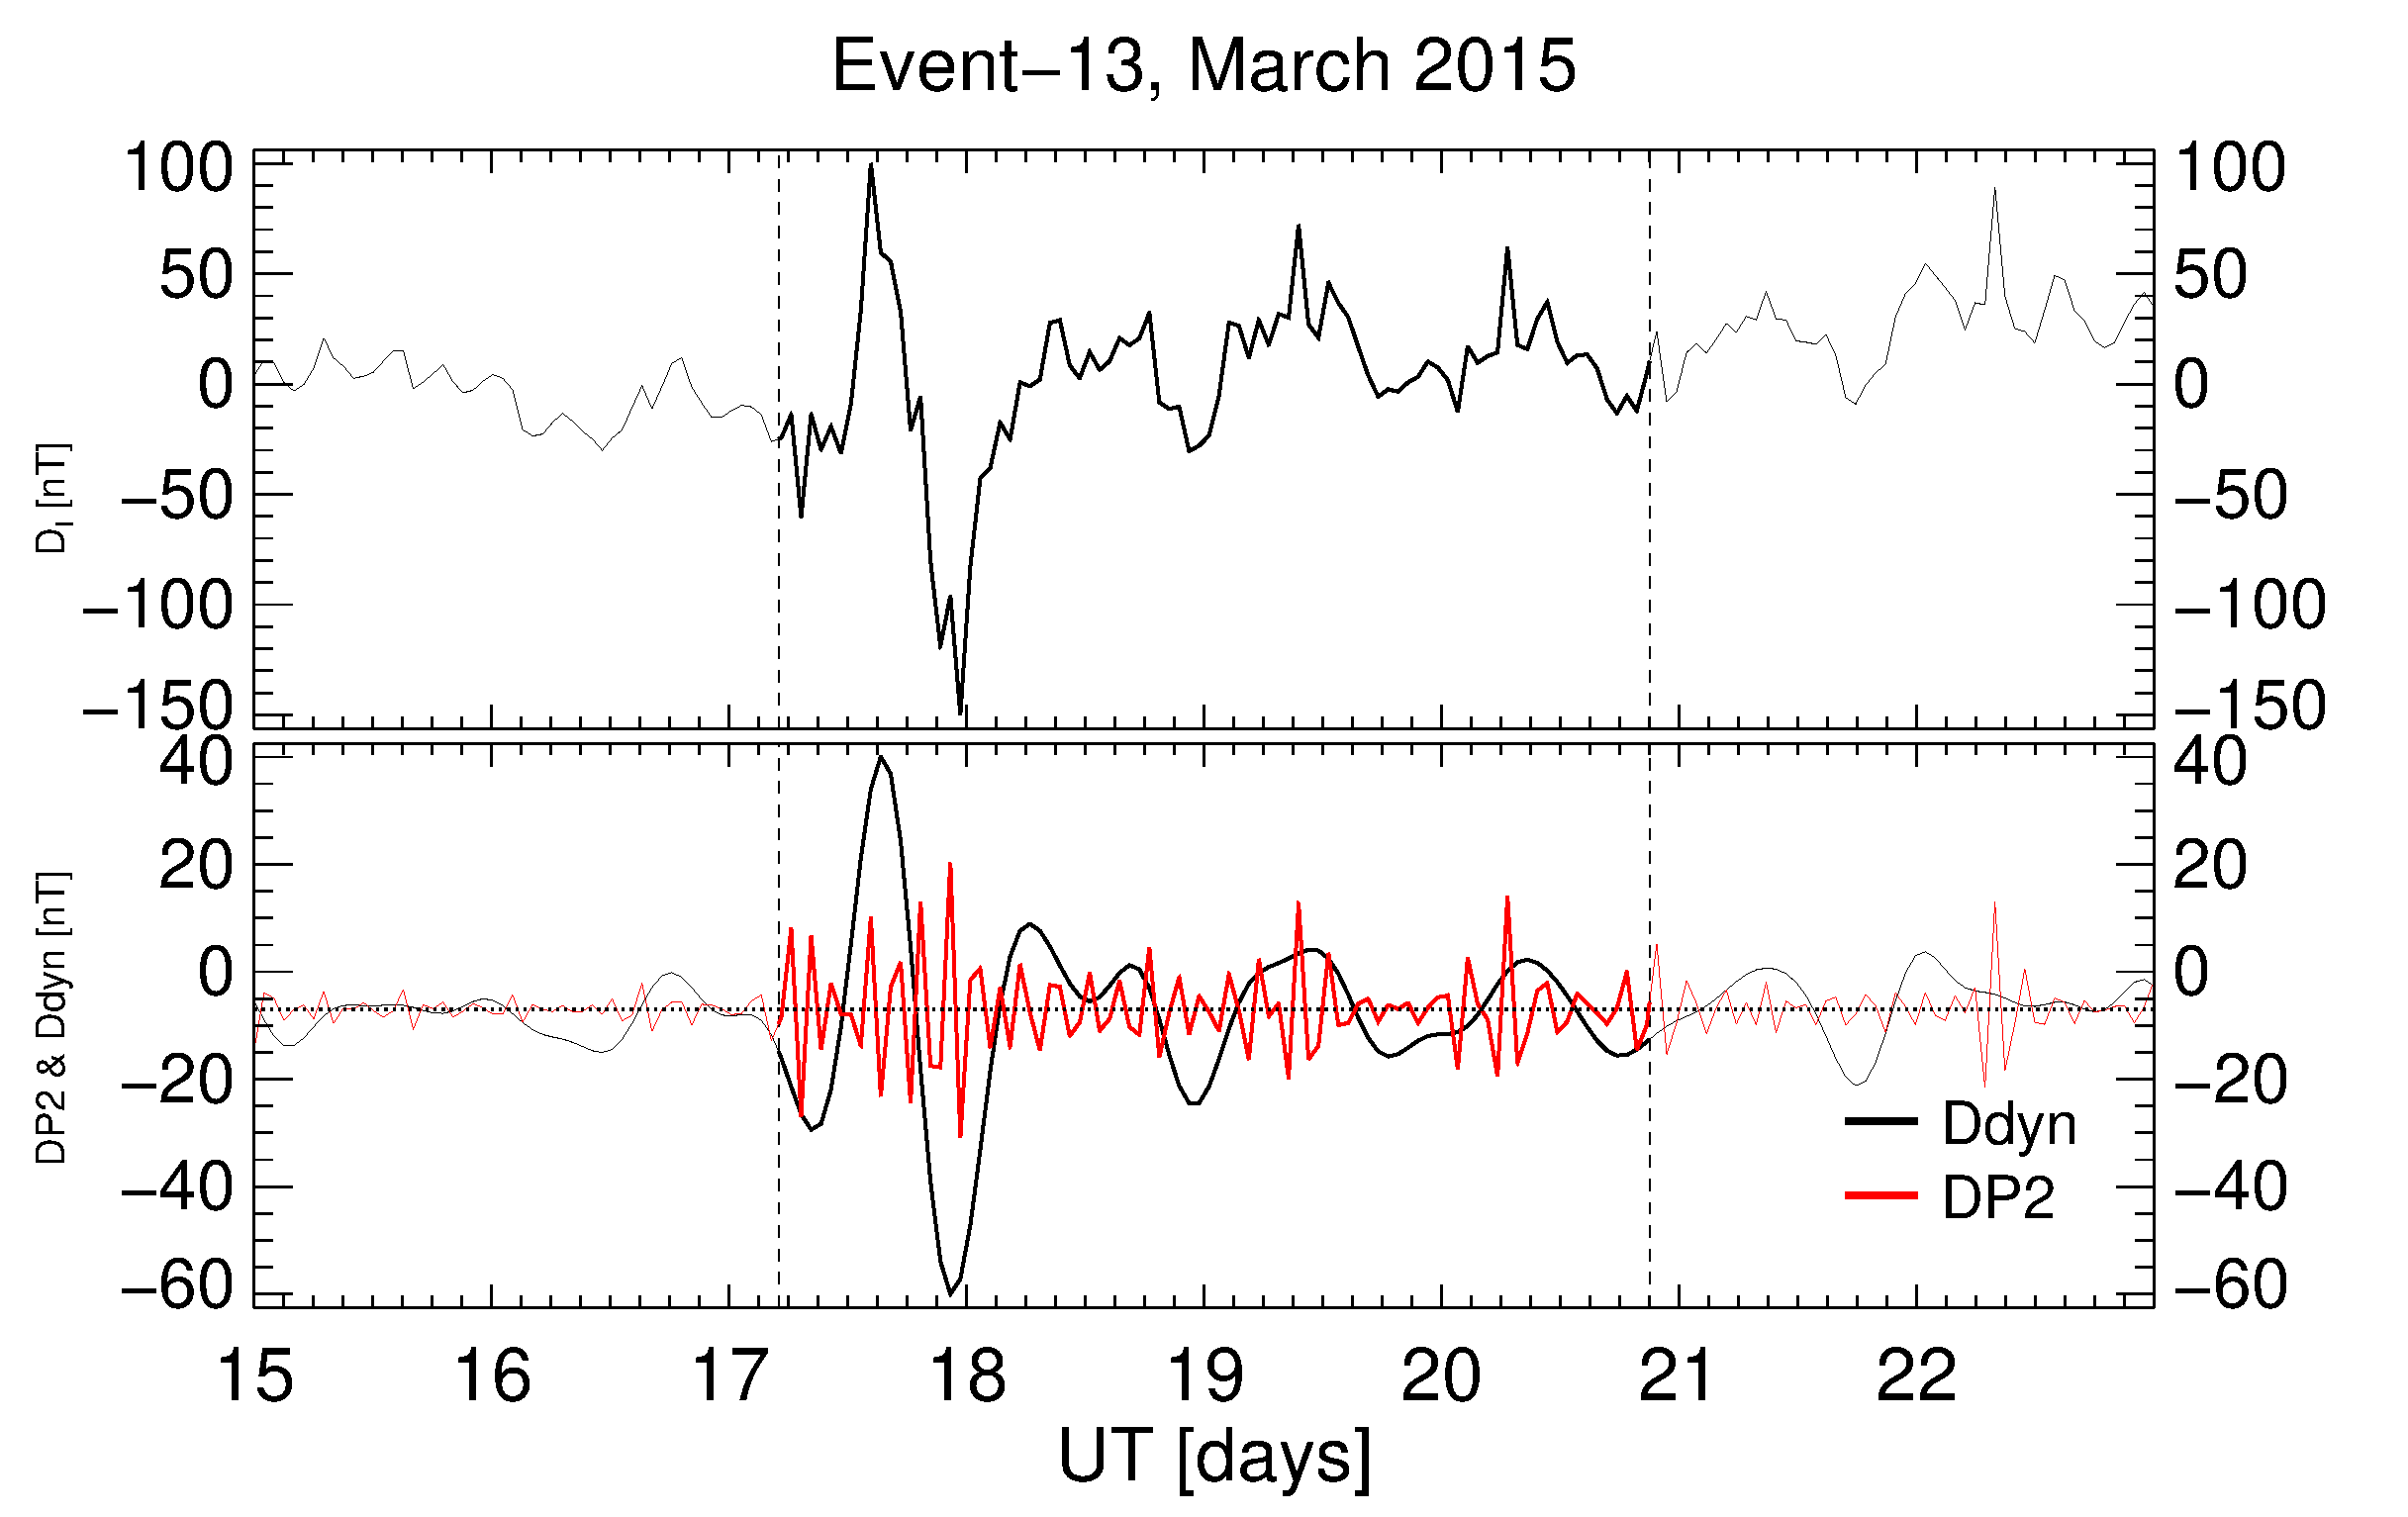
\includegraphics[width=6.0cm]{images/diono/iono_PI_V1_2015-03-15.eps}     
     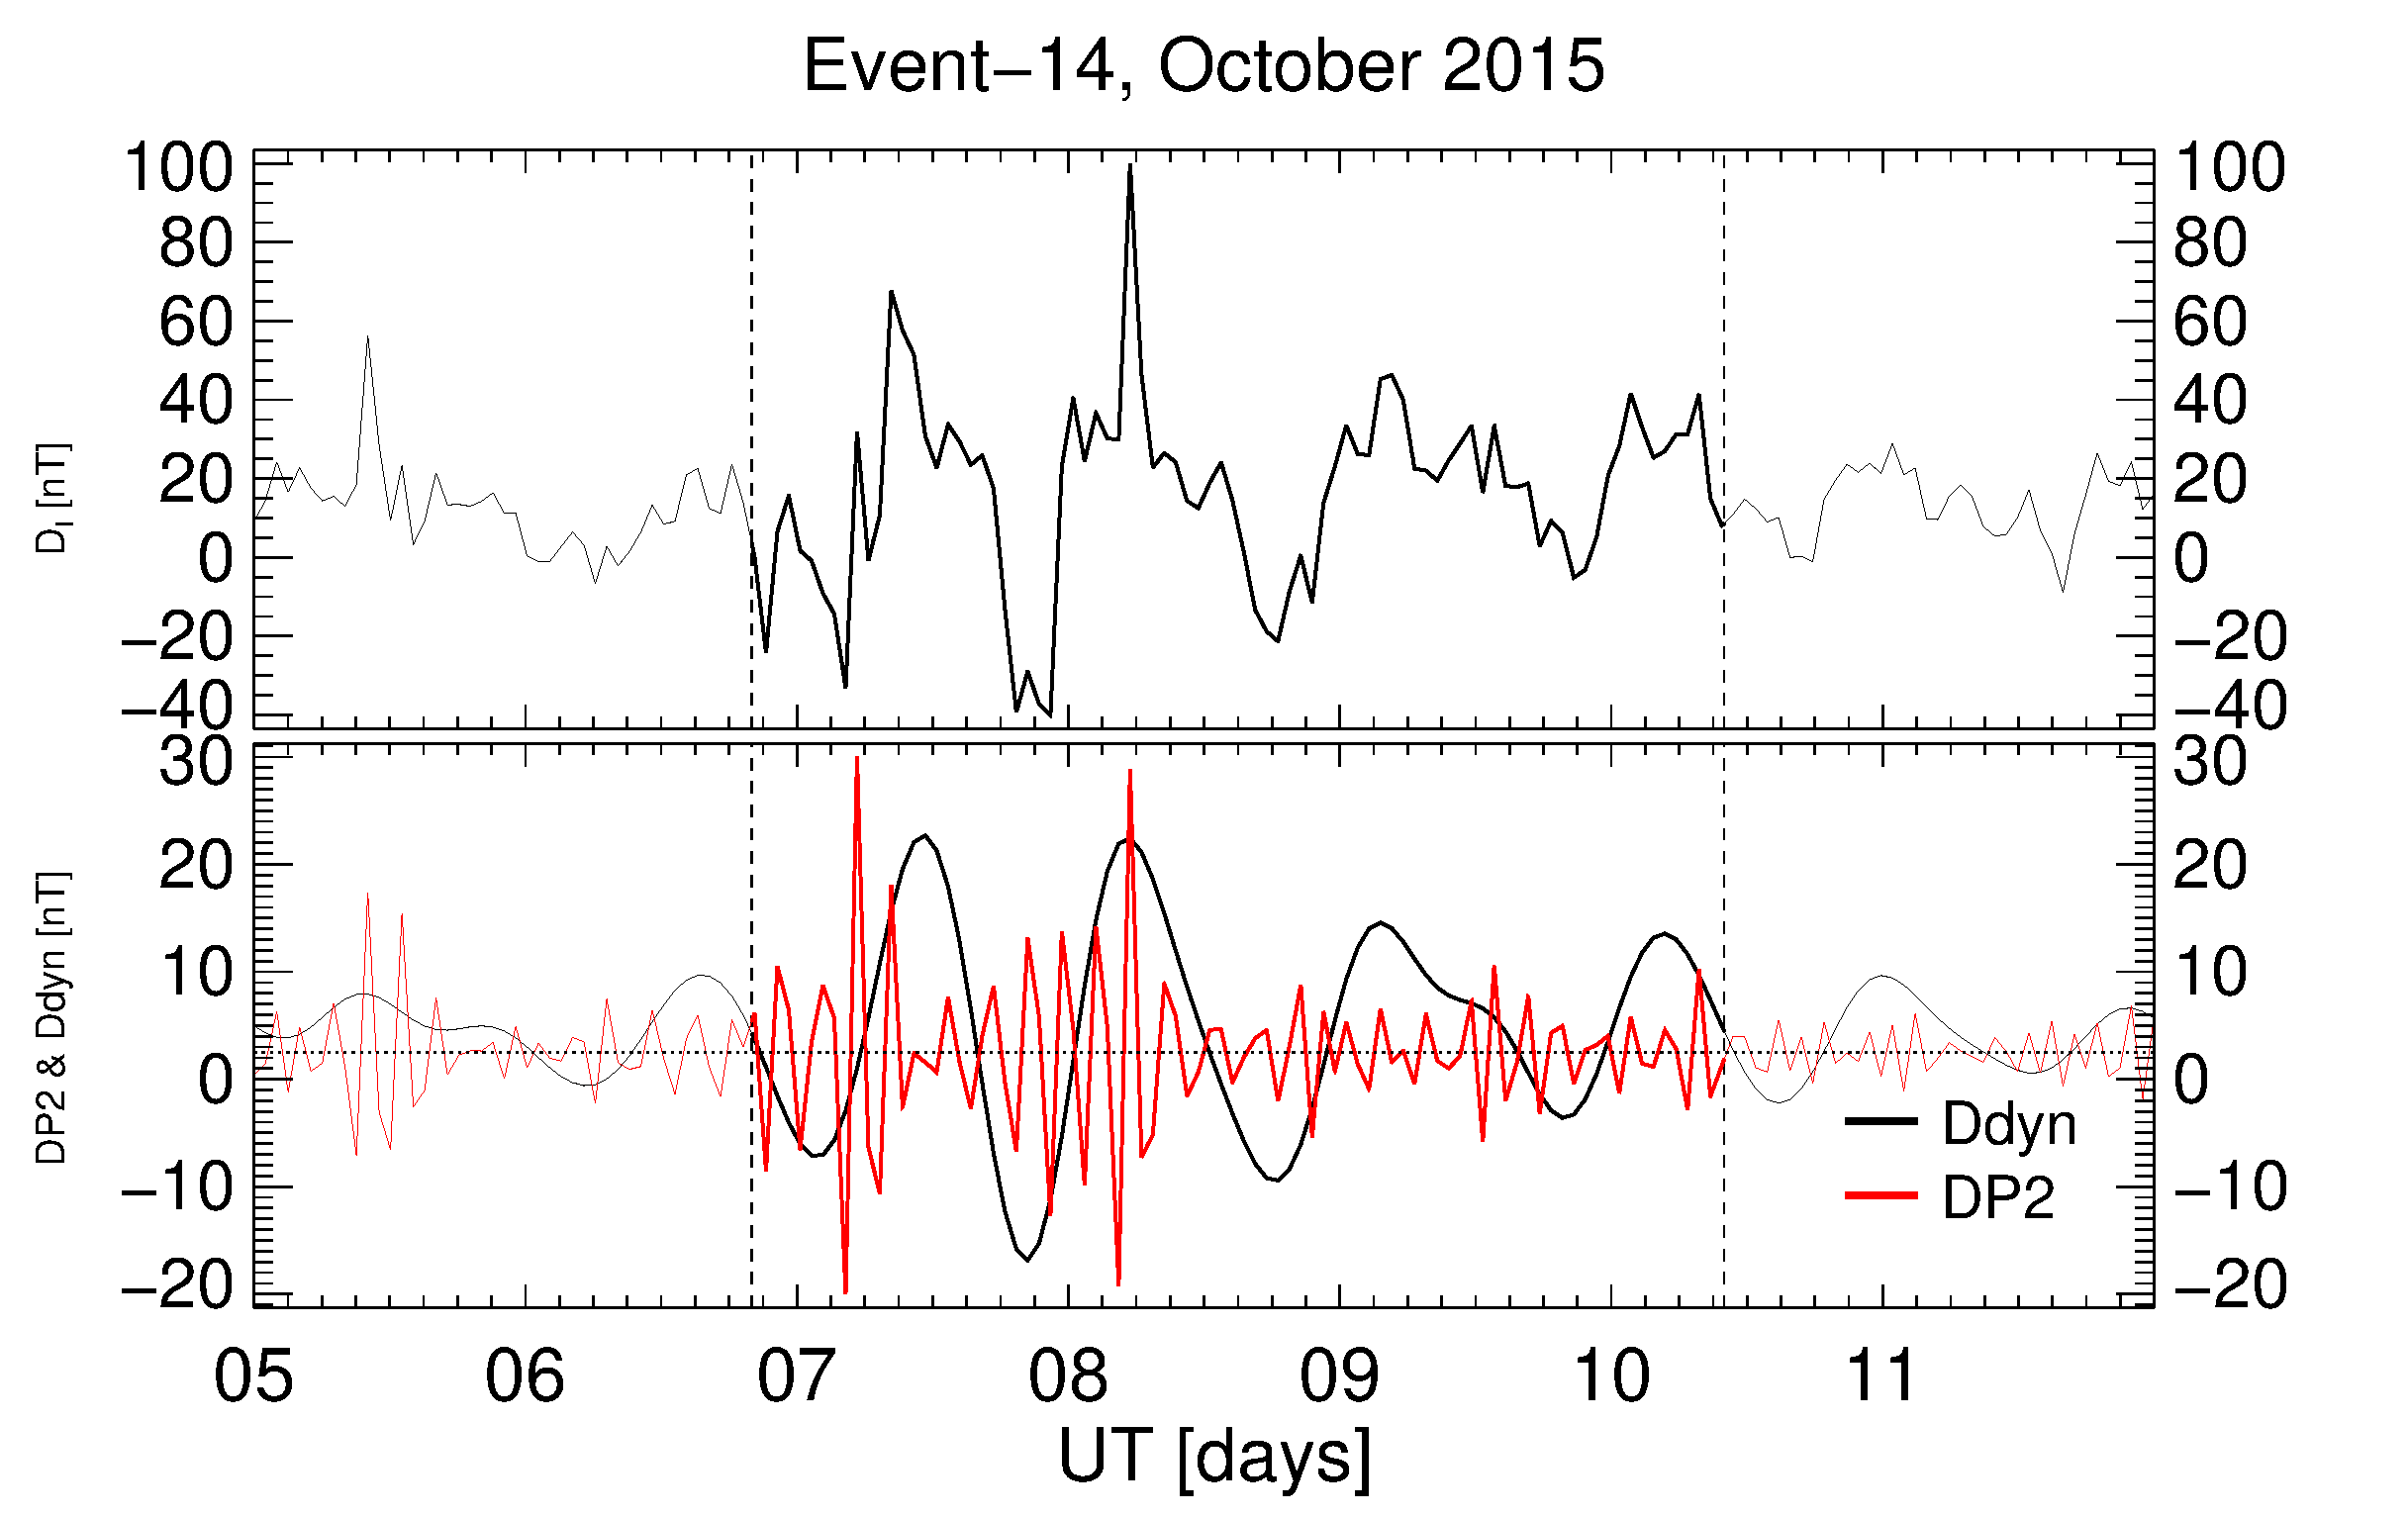
\includegraphics[width=6.0cm]{images/diono/iono_PI_V1_2015-10-05.eps}
     \centerline{\Large \bf   
      \hspace{0.275\textwidth}  \color{black}{}
       \hspace{0.295\textwidth}  \color{black}{}
         \hfill}
      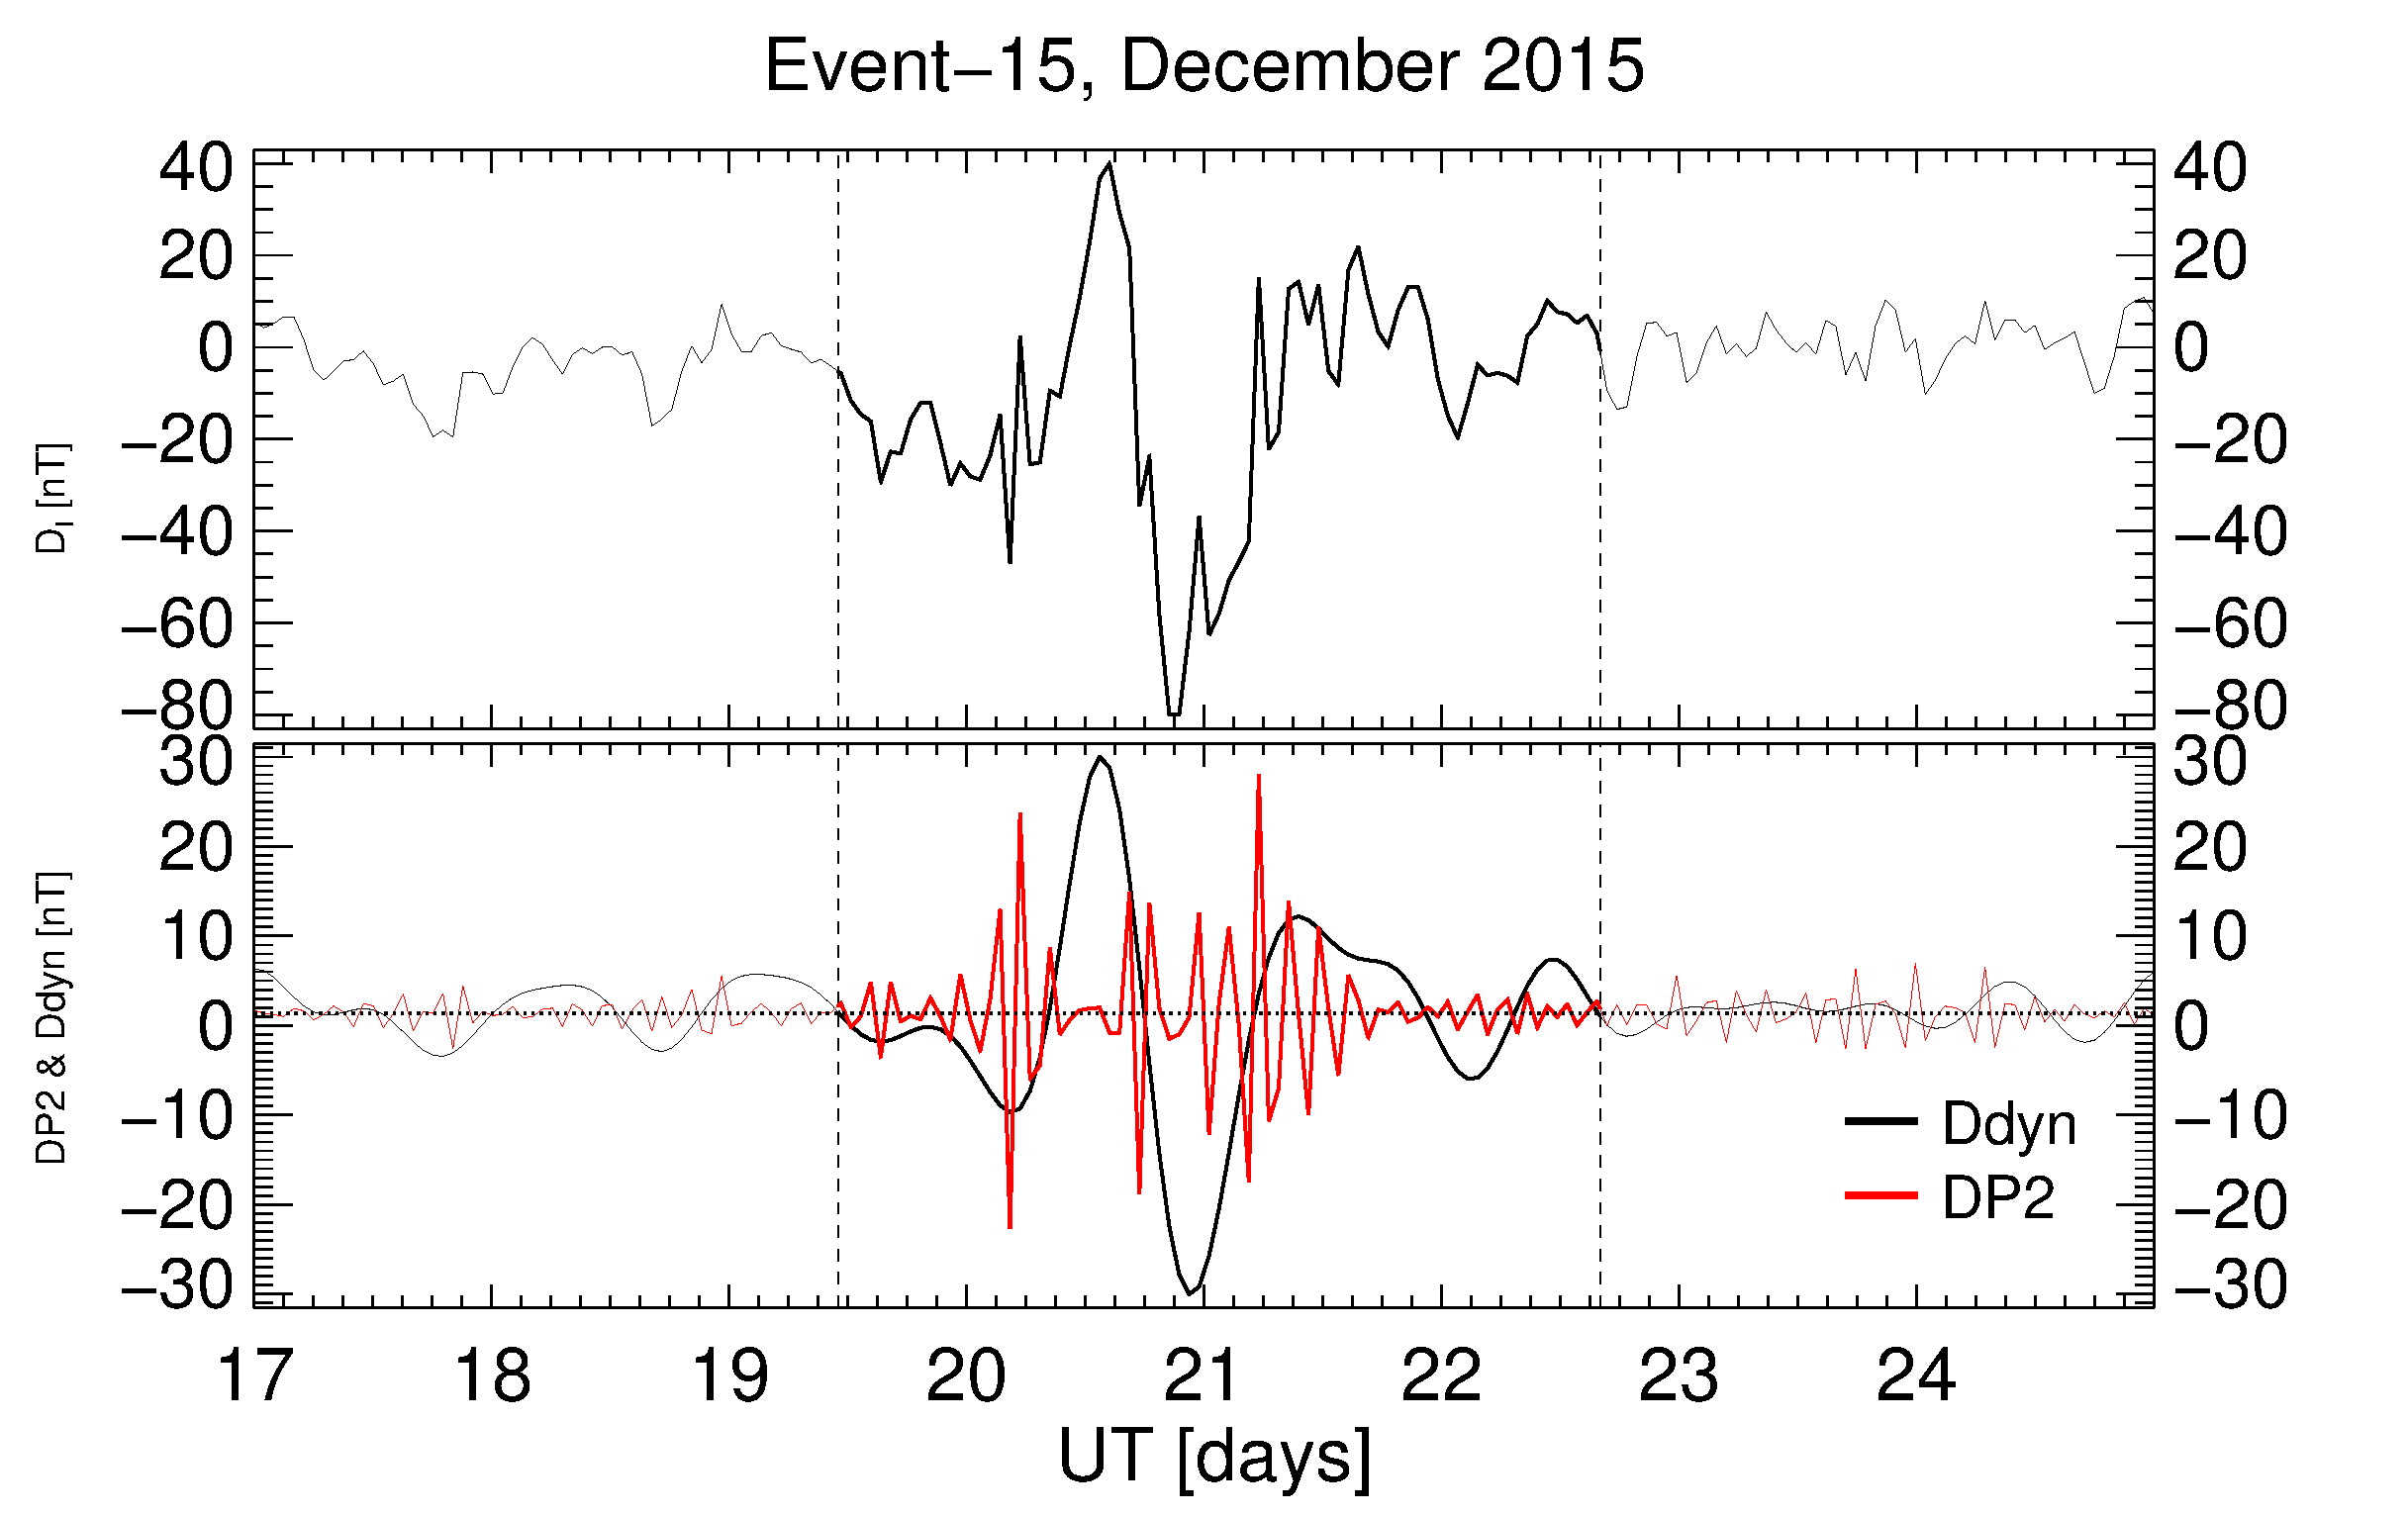
\includegraphics[width=6.0cm]{images/diono/iono_PI_V1_2015-12-17.eps}     
      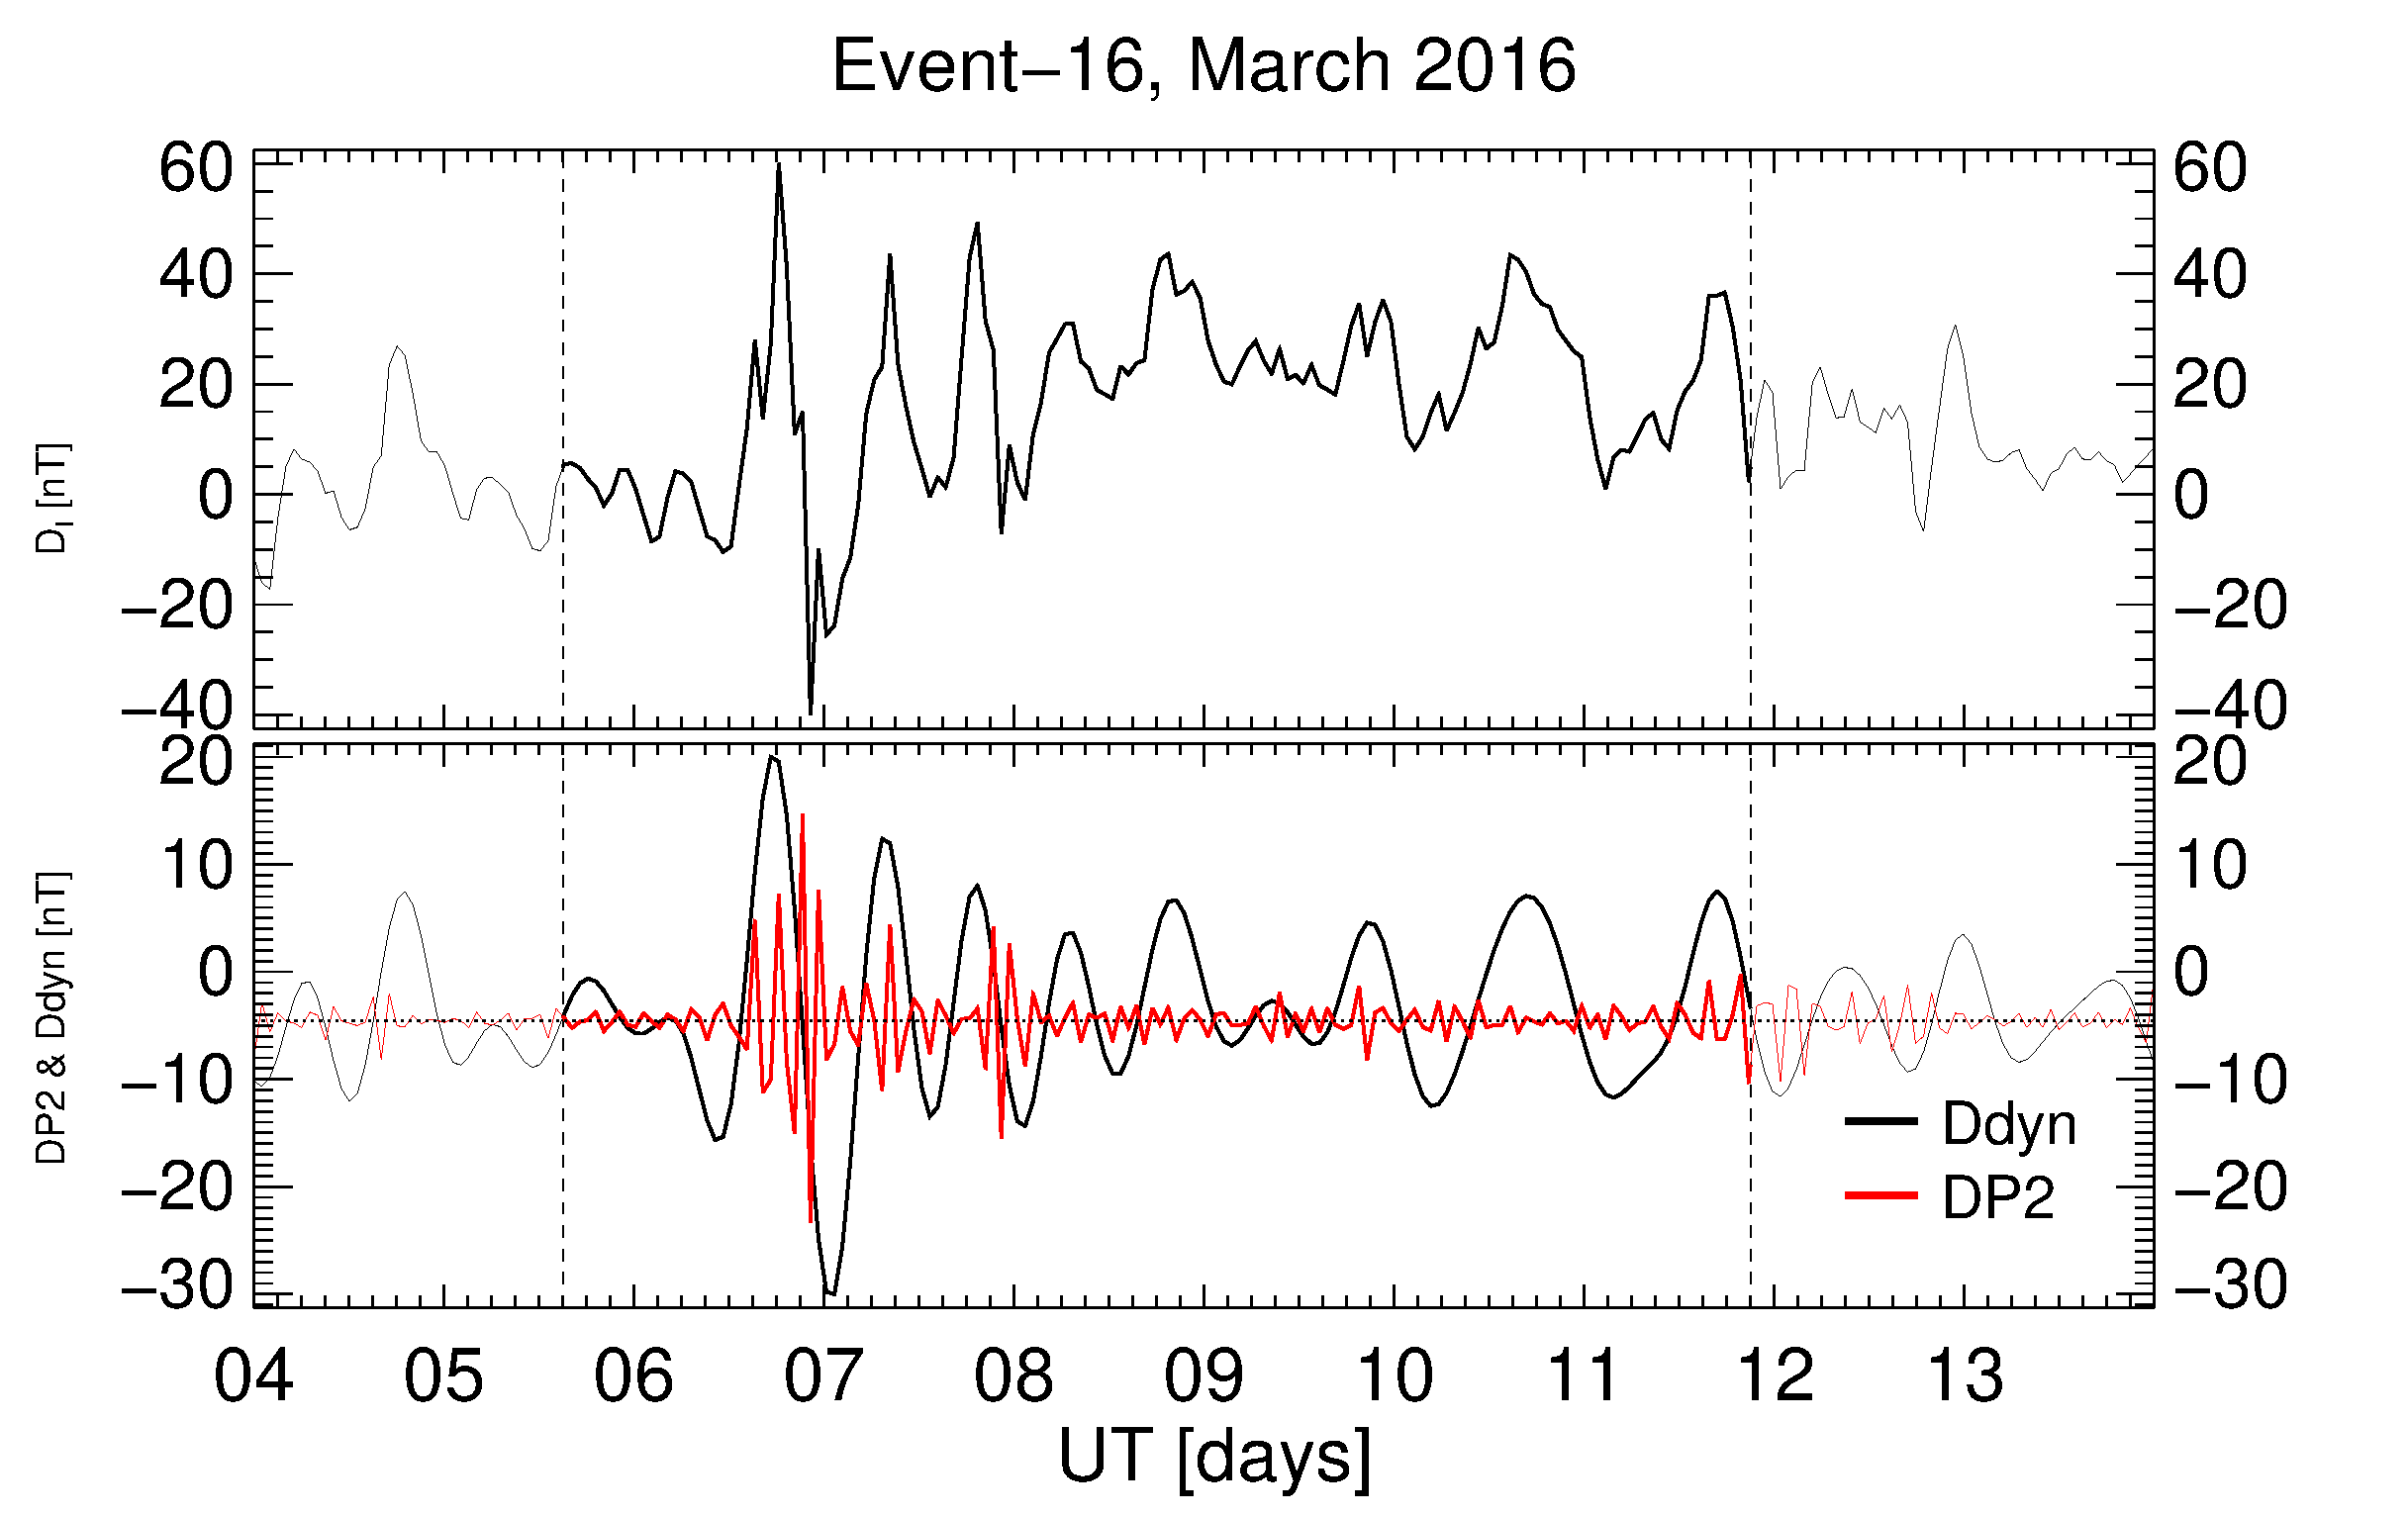
\includegraphics[width=6.0cm]{images/diono/iono_PI_V1_2016-03-04.eps}
       \centerline{\Large \bf   
      \hspace{0.275\textwidth}  \color{black}{}
       \hspace{0.295\textwidth}  \color{black}{}
         \hfill}
       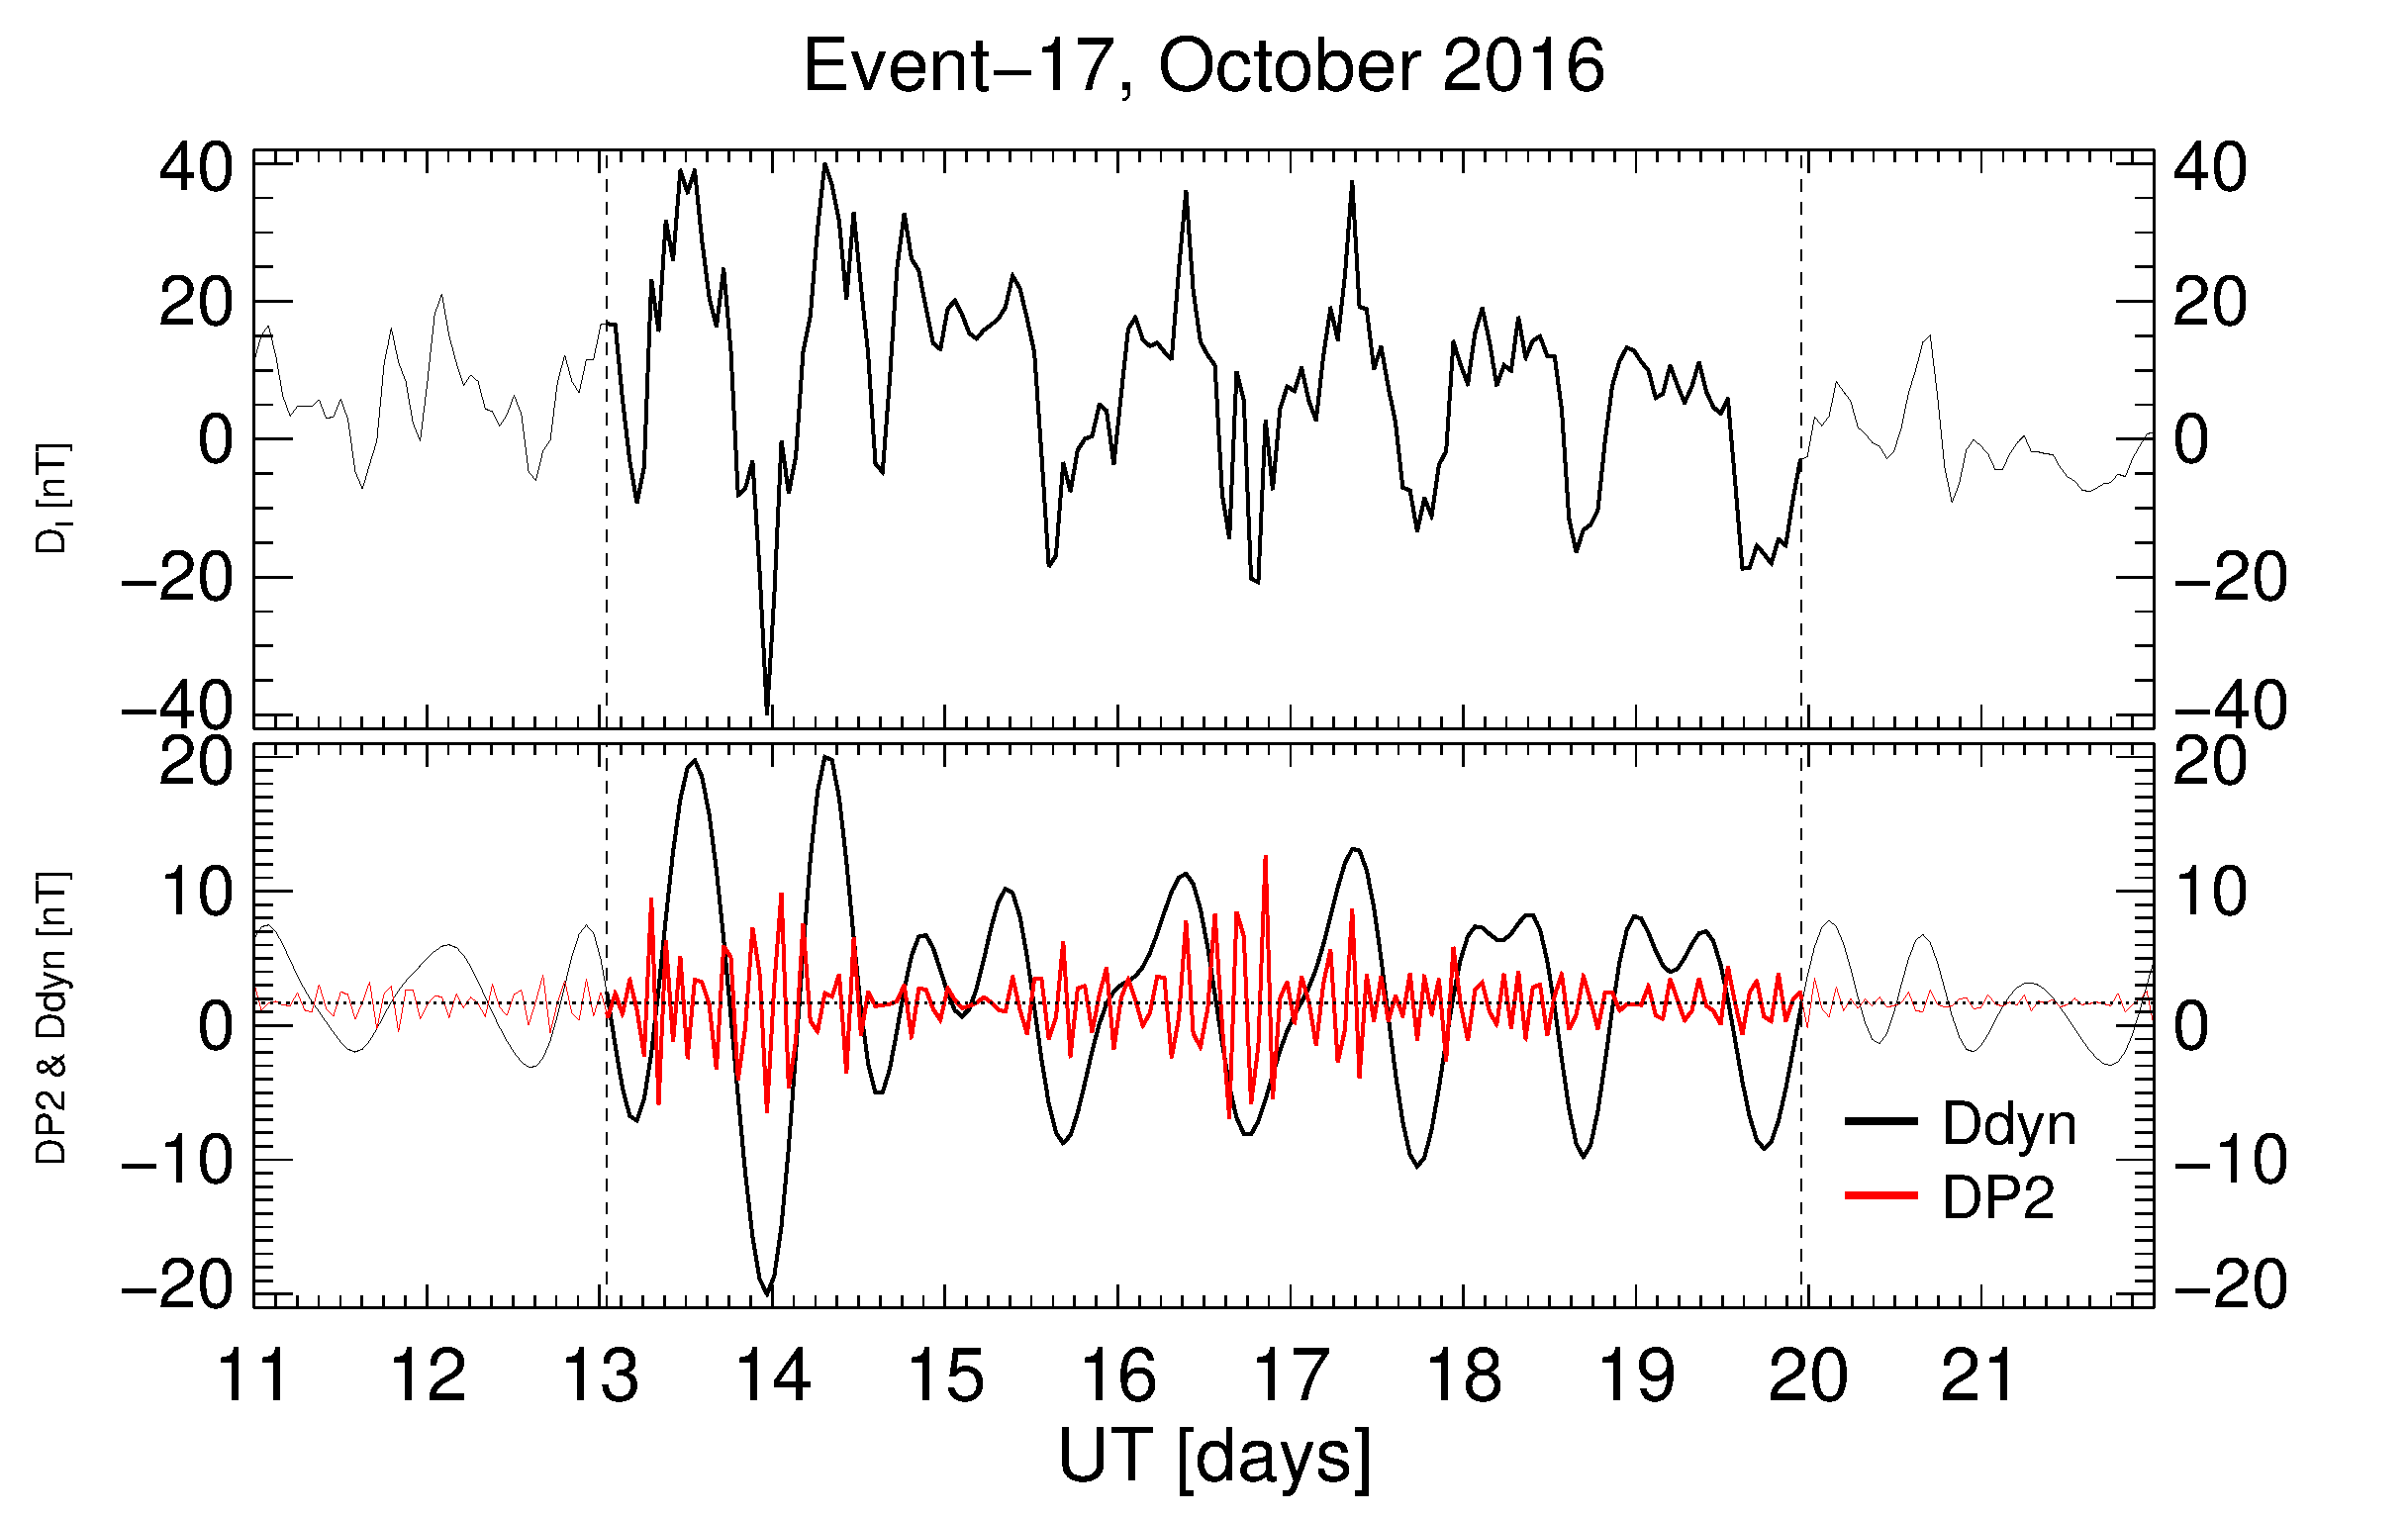
\includegraphics[width=6.0cm]{images/diono/iono_PI_V1_2016-10-11.eps}     
       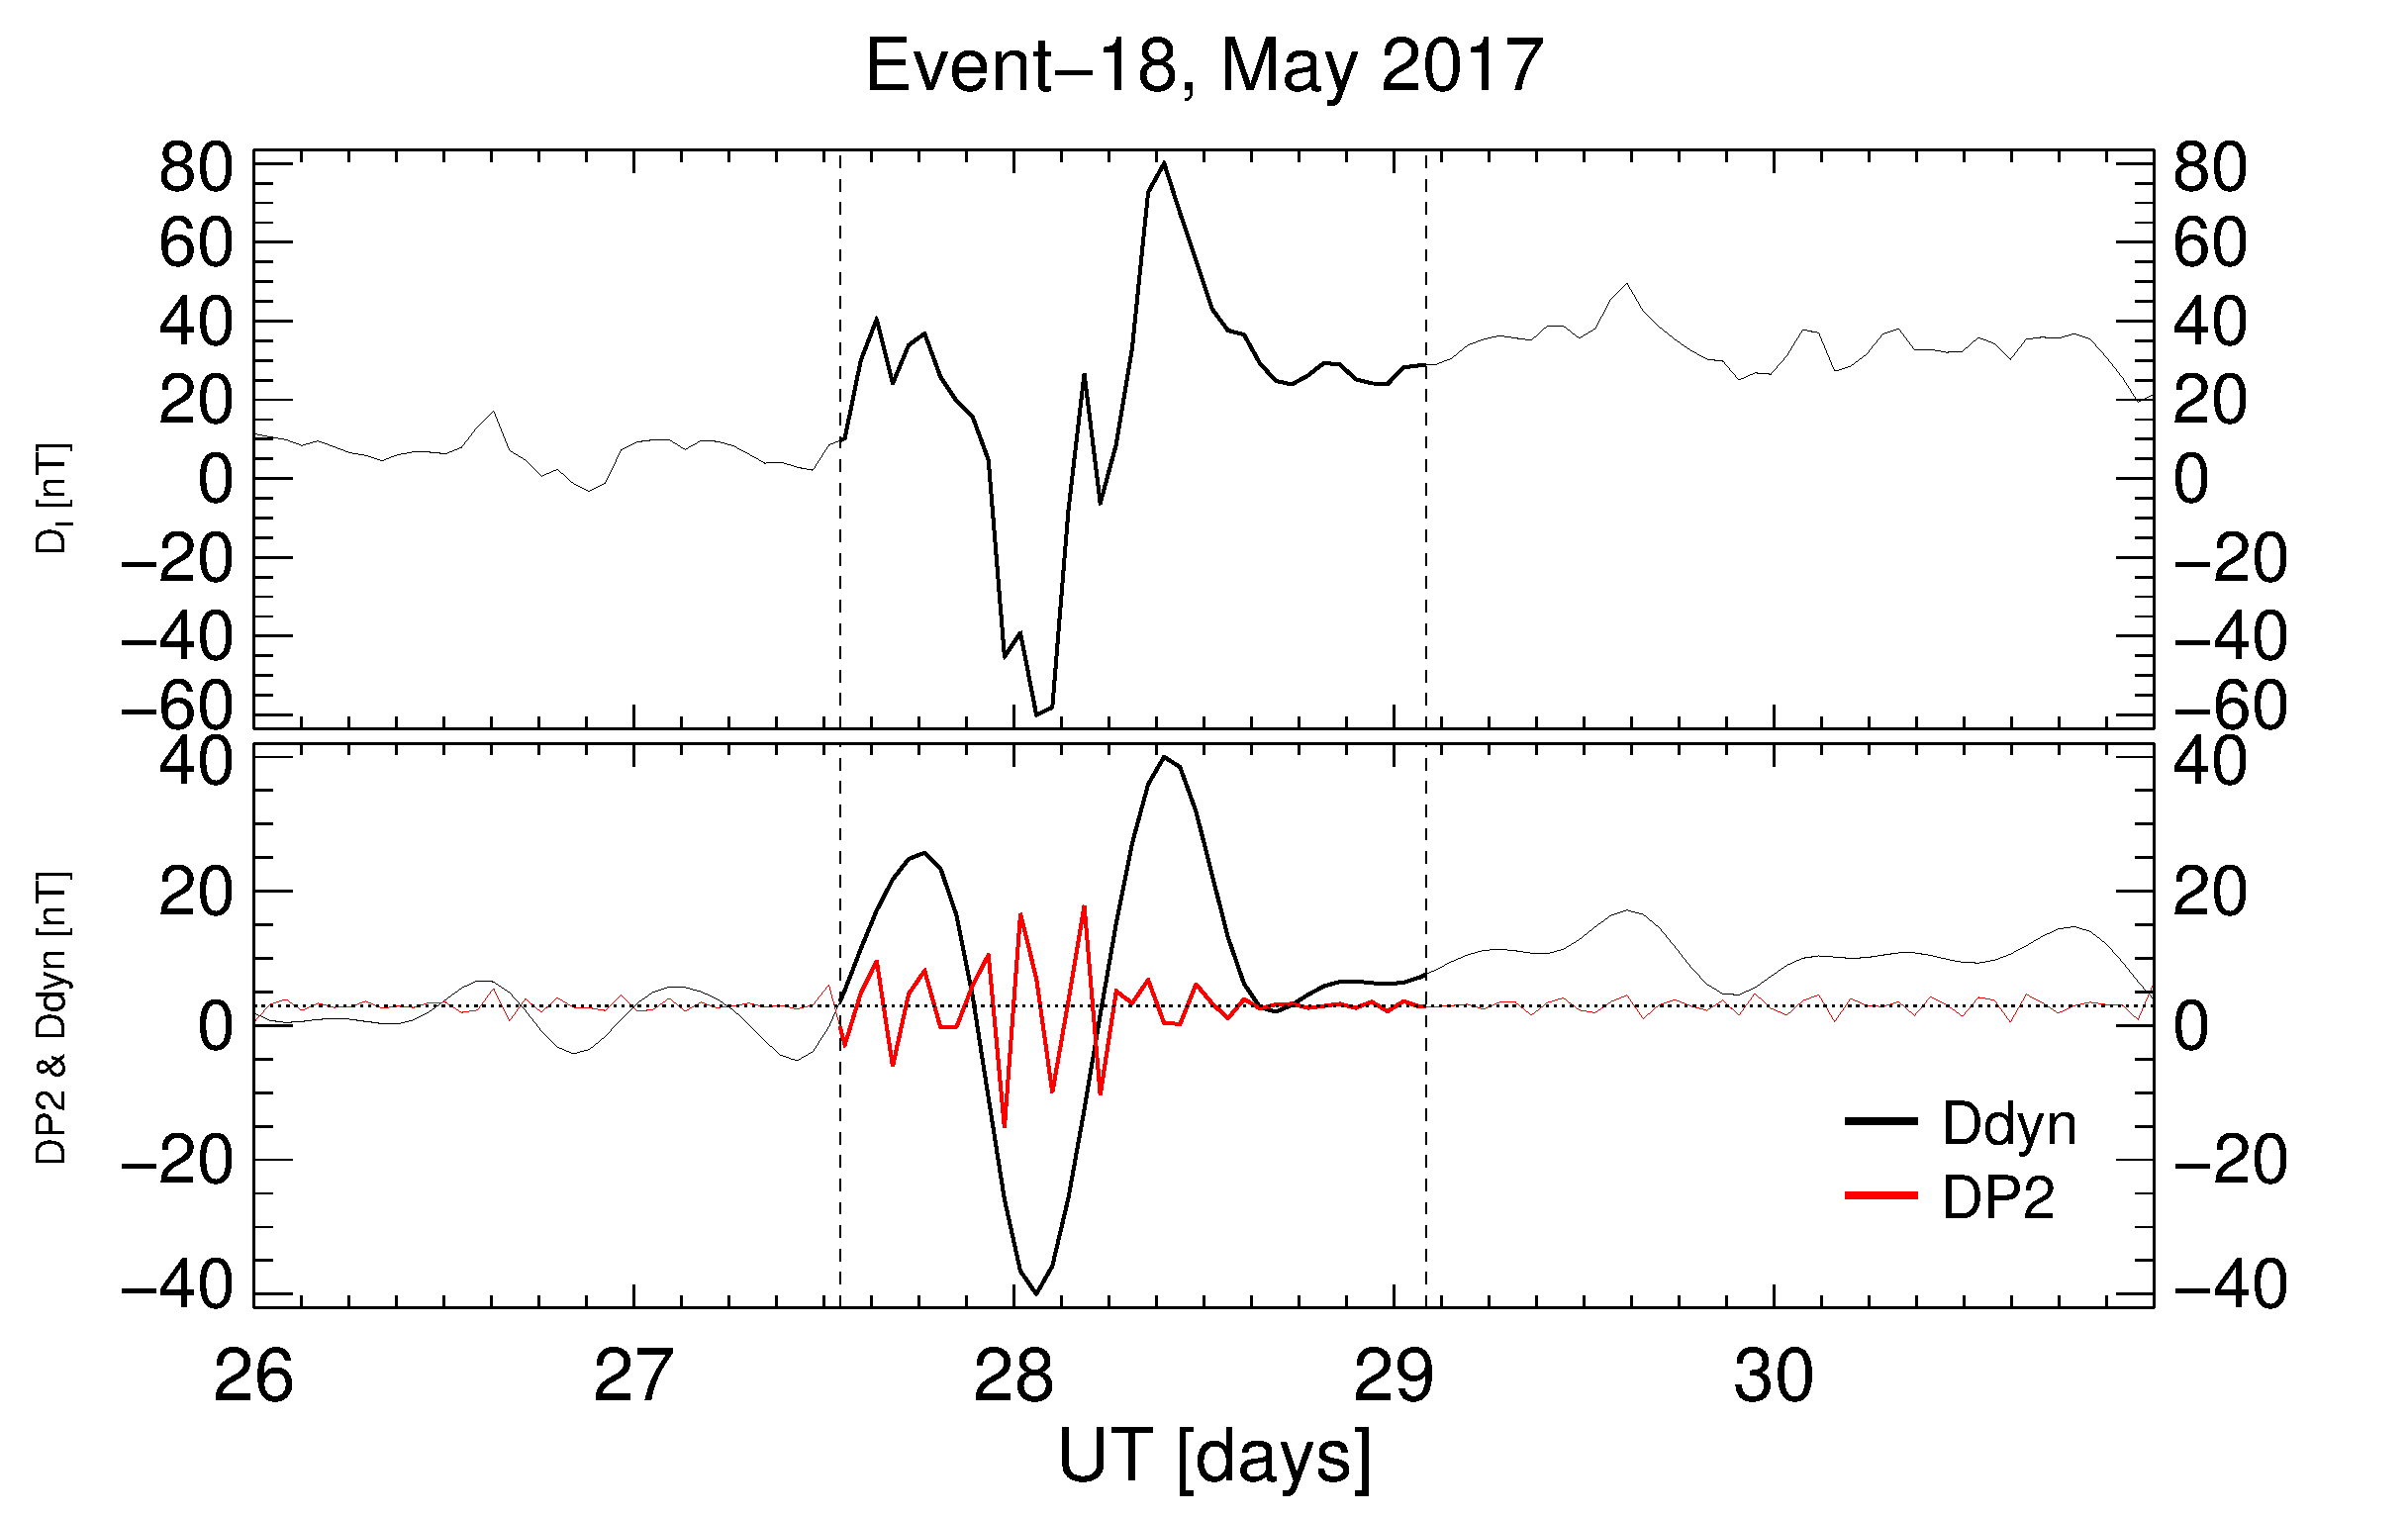
\includegraphics[width=6.0cm]{images/diono/iono_PI_V1_2017-05-26.eps}

       \centerline{\Large \bf   
      \hspace{0.275\textwidth}  \color{black}{}
       \hspace{0.295\textwidth}  \color{black}{}
         \hfill}
       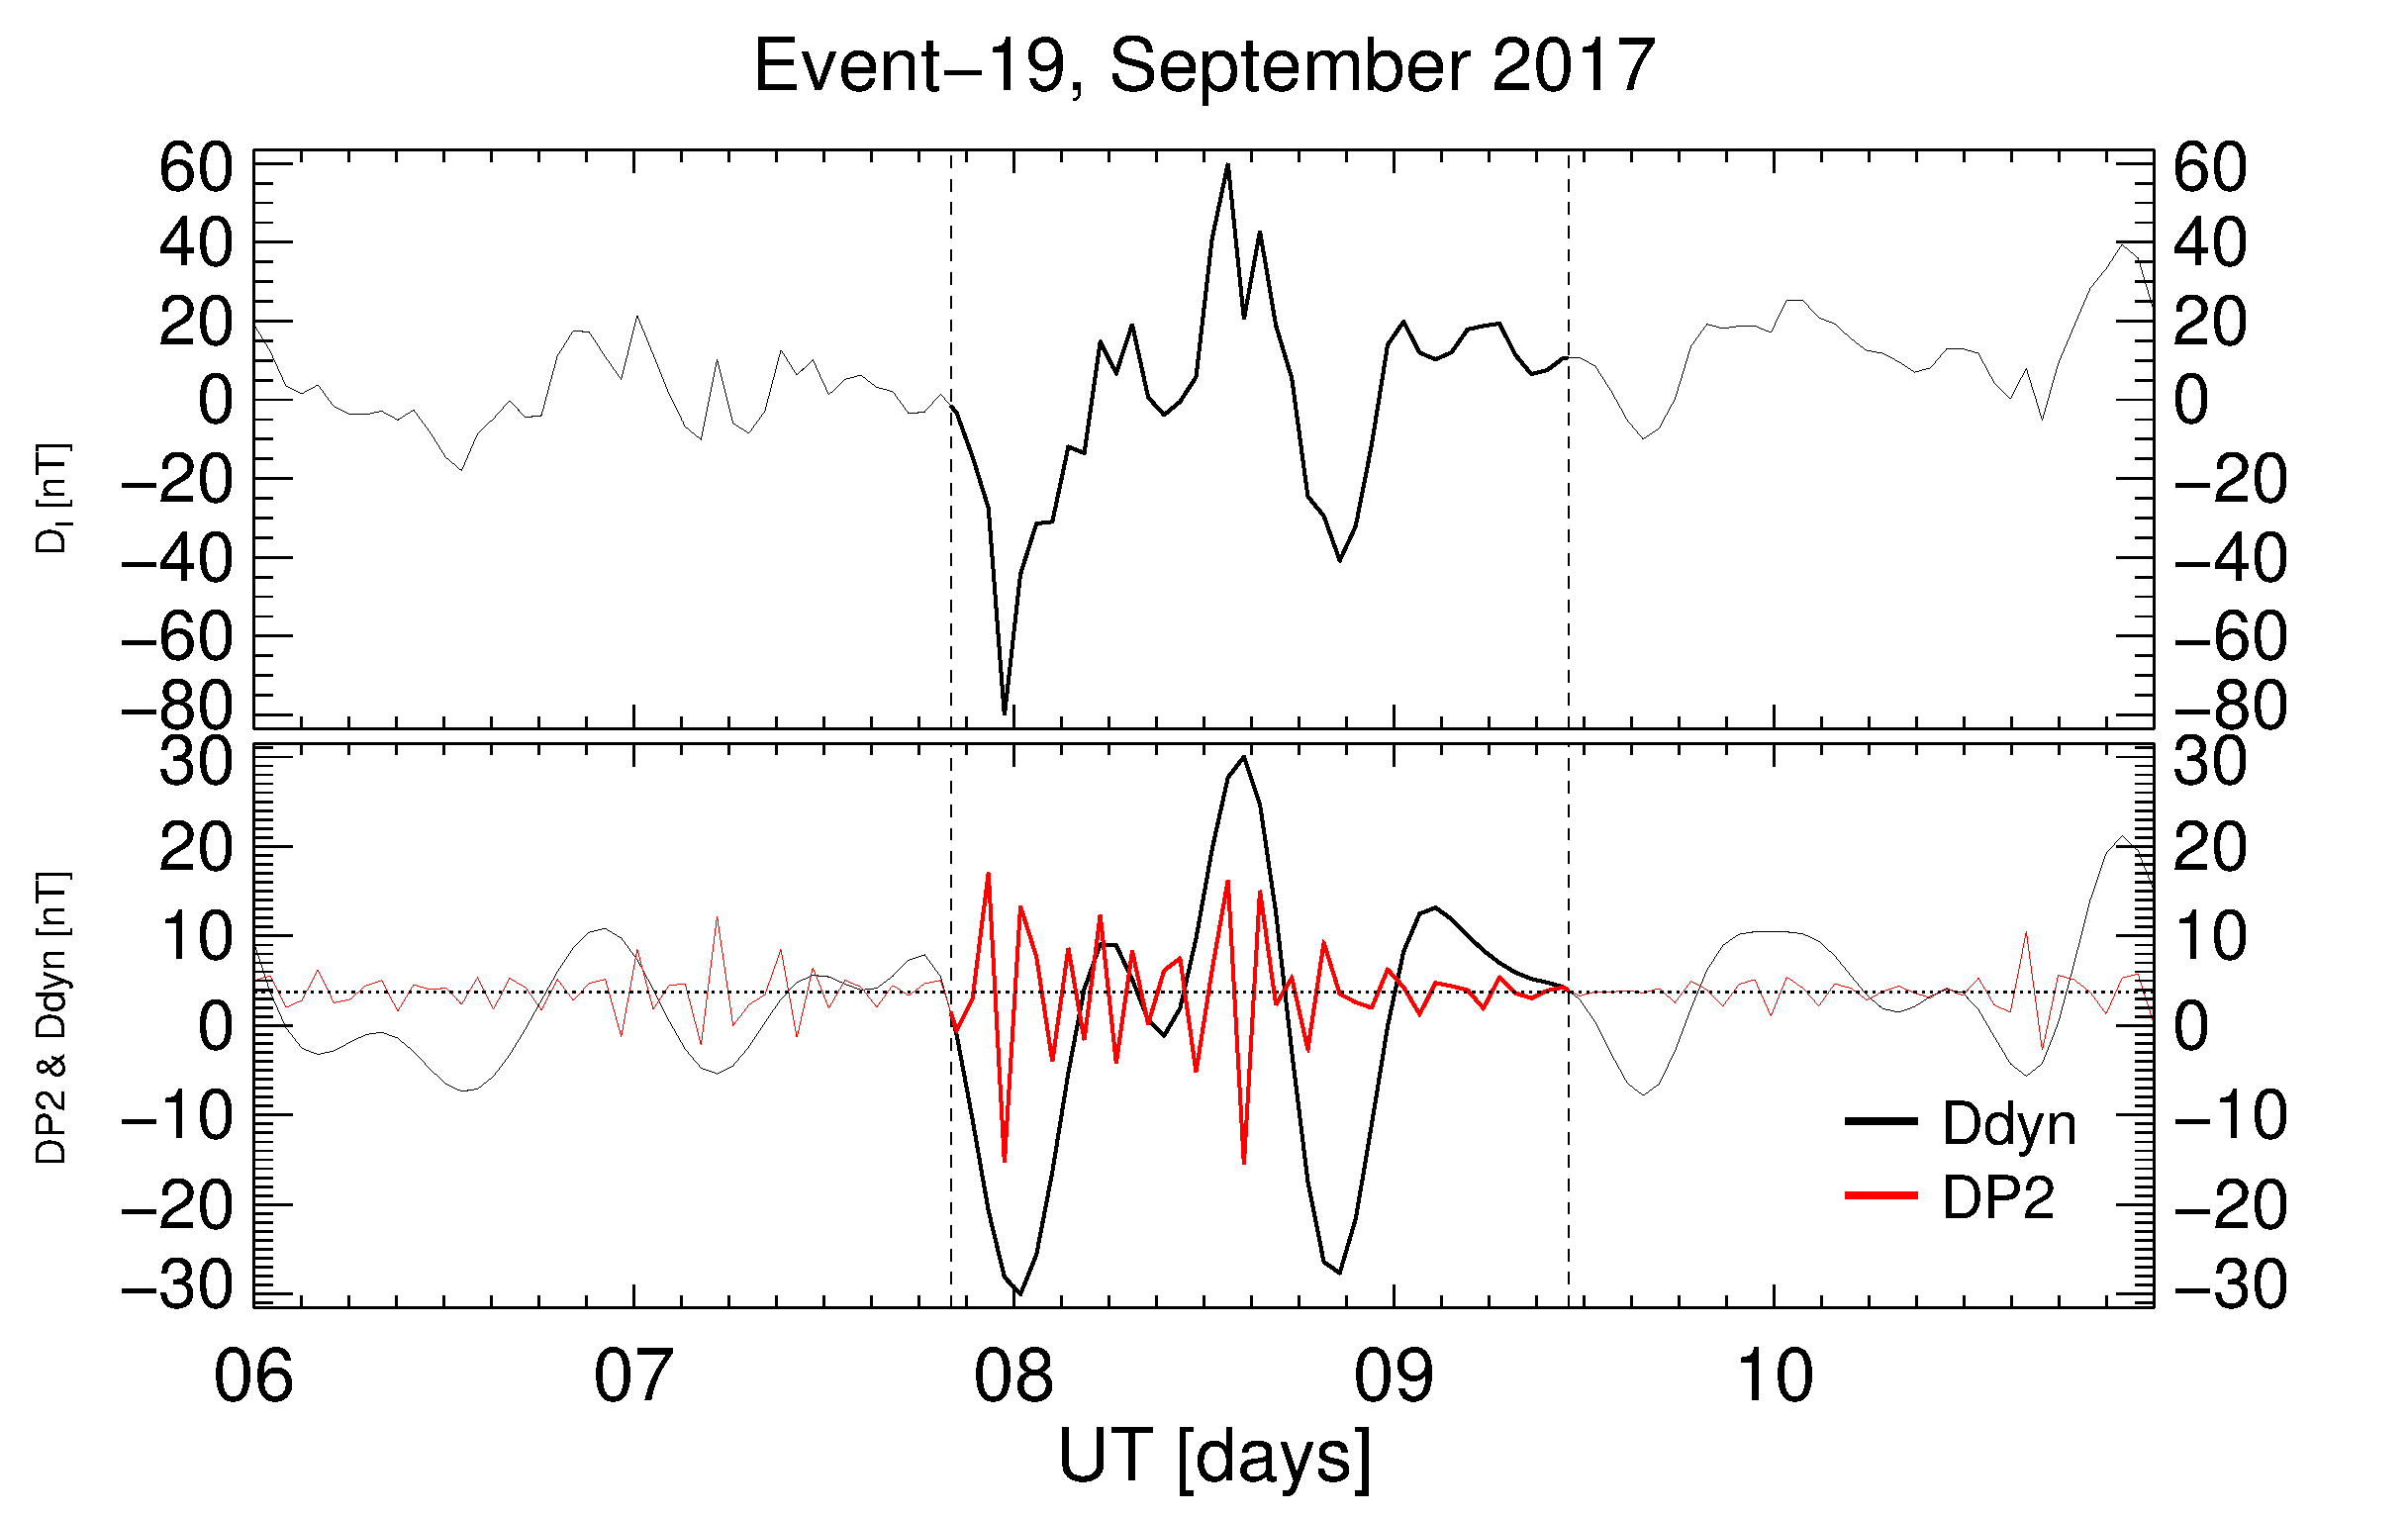
\includegraphics[width=6.0cm]{images/diono/iono_PI_V1_2017-09-06.eps}     
       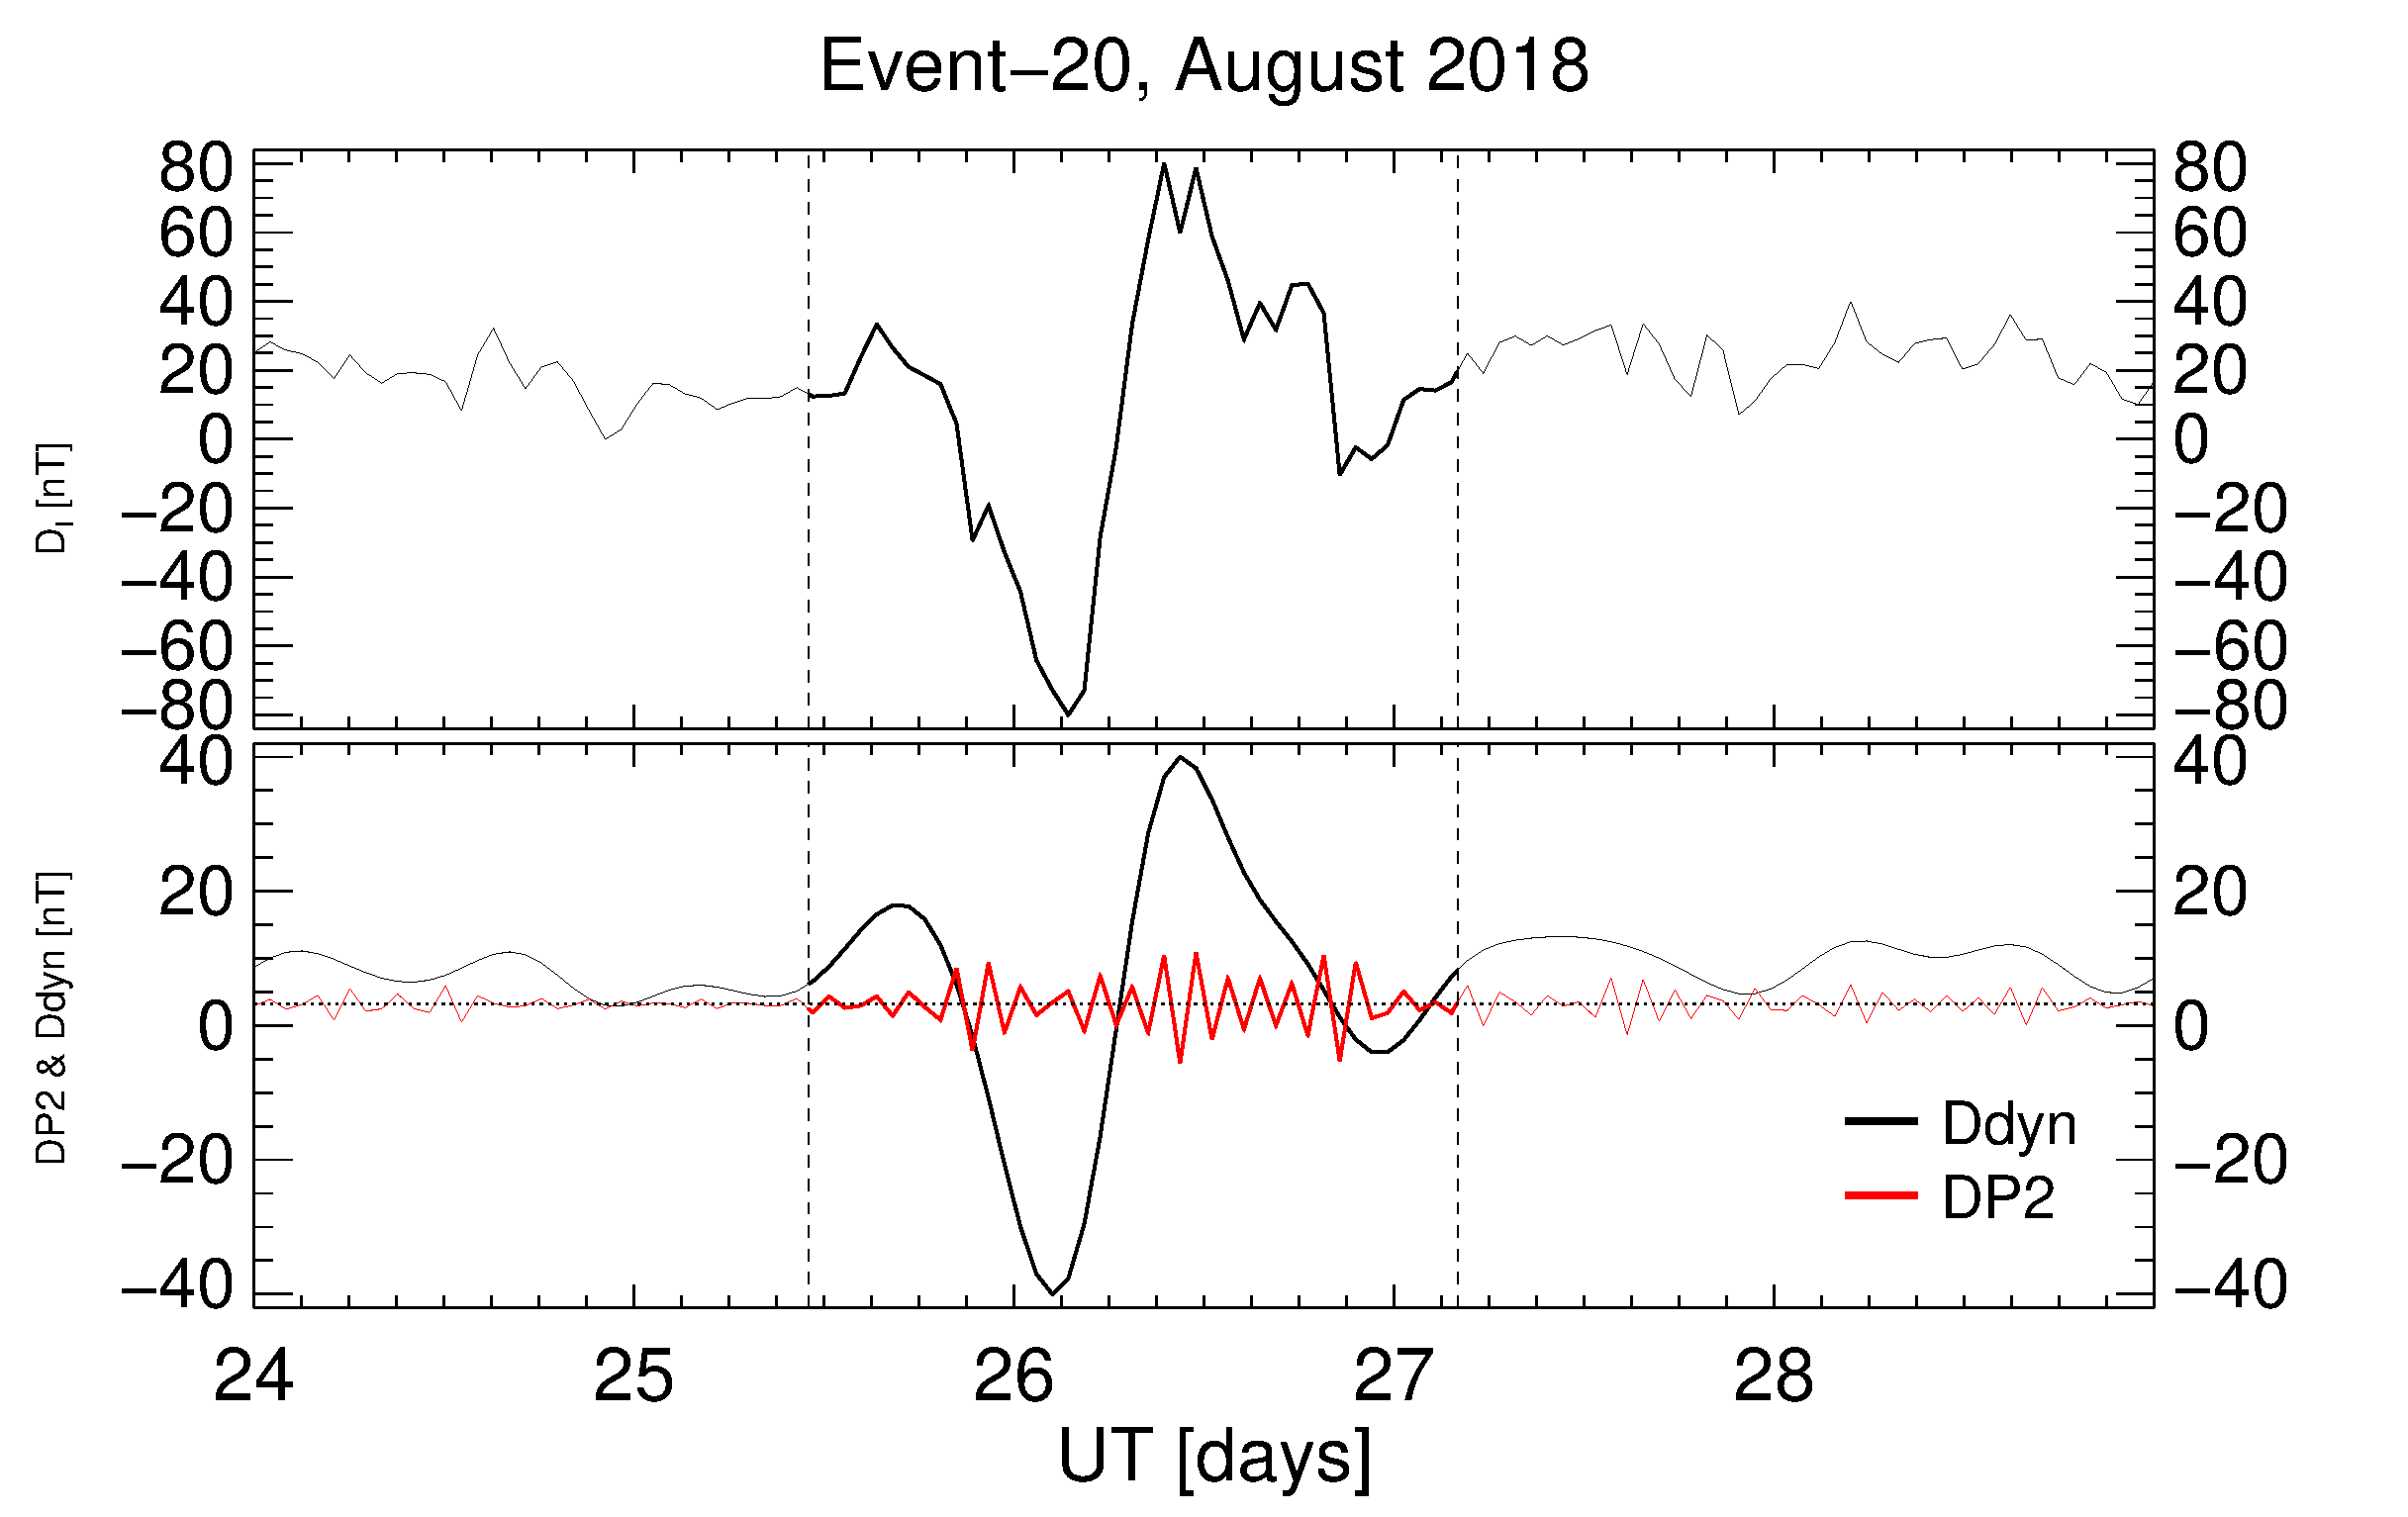
\includegraphics[width=6.0cm]{images/diono/iono_PI_V1_2018-08-24.eps}
       
       \caption{Ionospheric Magnetic Disturbance contribution (top panels) and the isolated Ddyn and DP2 geomagnetic contribution (bottom panels).}
    \label{fig:iono_resp3}
\end{figure*}


\begin{figure*}[h!]
    \centering
    \centerline{\Large \bf   
      %\hspace{0.18\textwidth}  \color{black}{\Large{Res}}
       %\hspace{0.28\textwidth}  \color{black}{\Large{Res+TC}}
         \hfill}
          \centerline{\Large \bf   
      \hspace{0.26\textwidth}  \color{black}{}
       \hspace{0.31\textwidth}  \color{black}{}
         \hfill}
     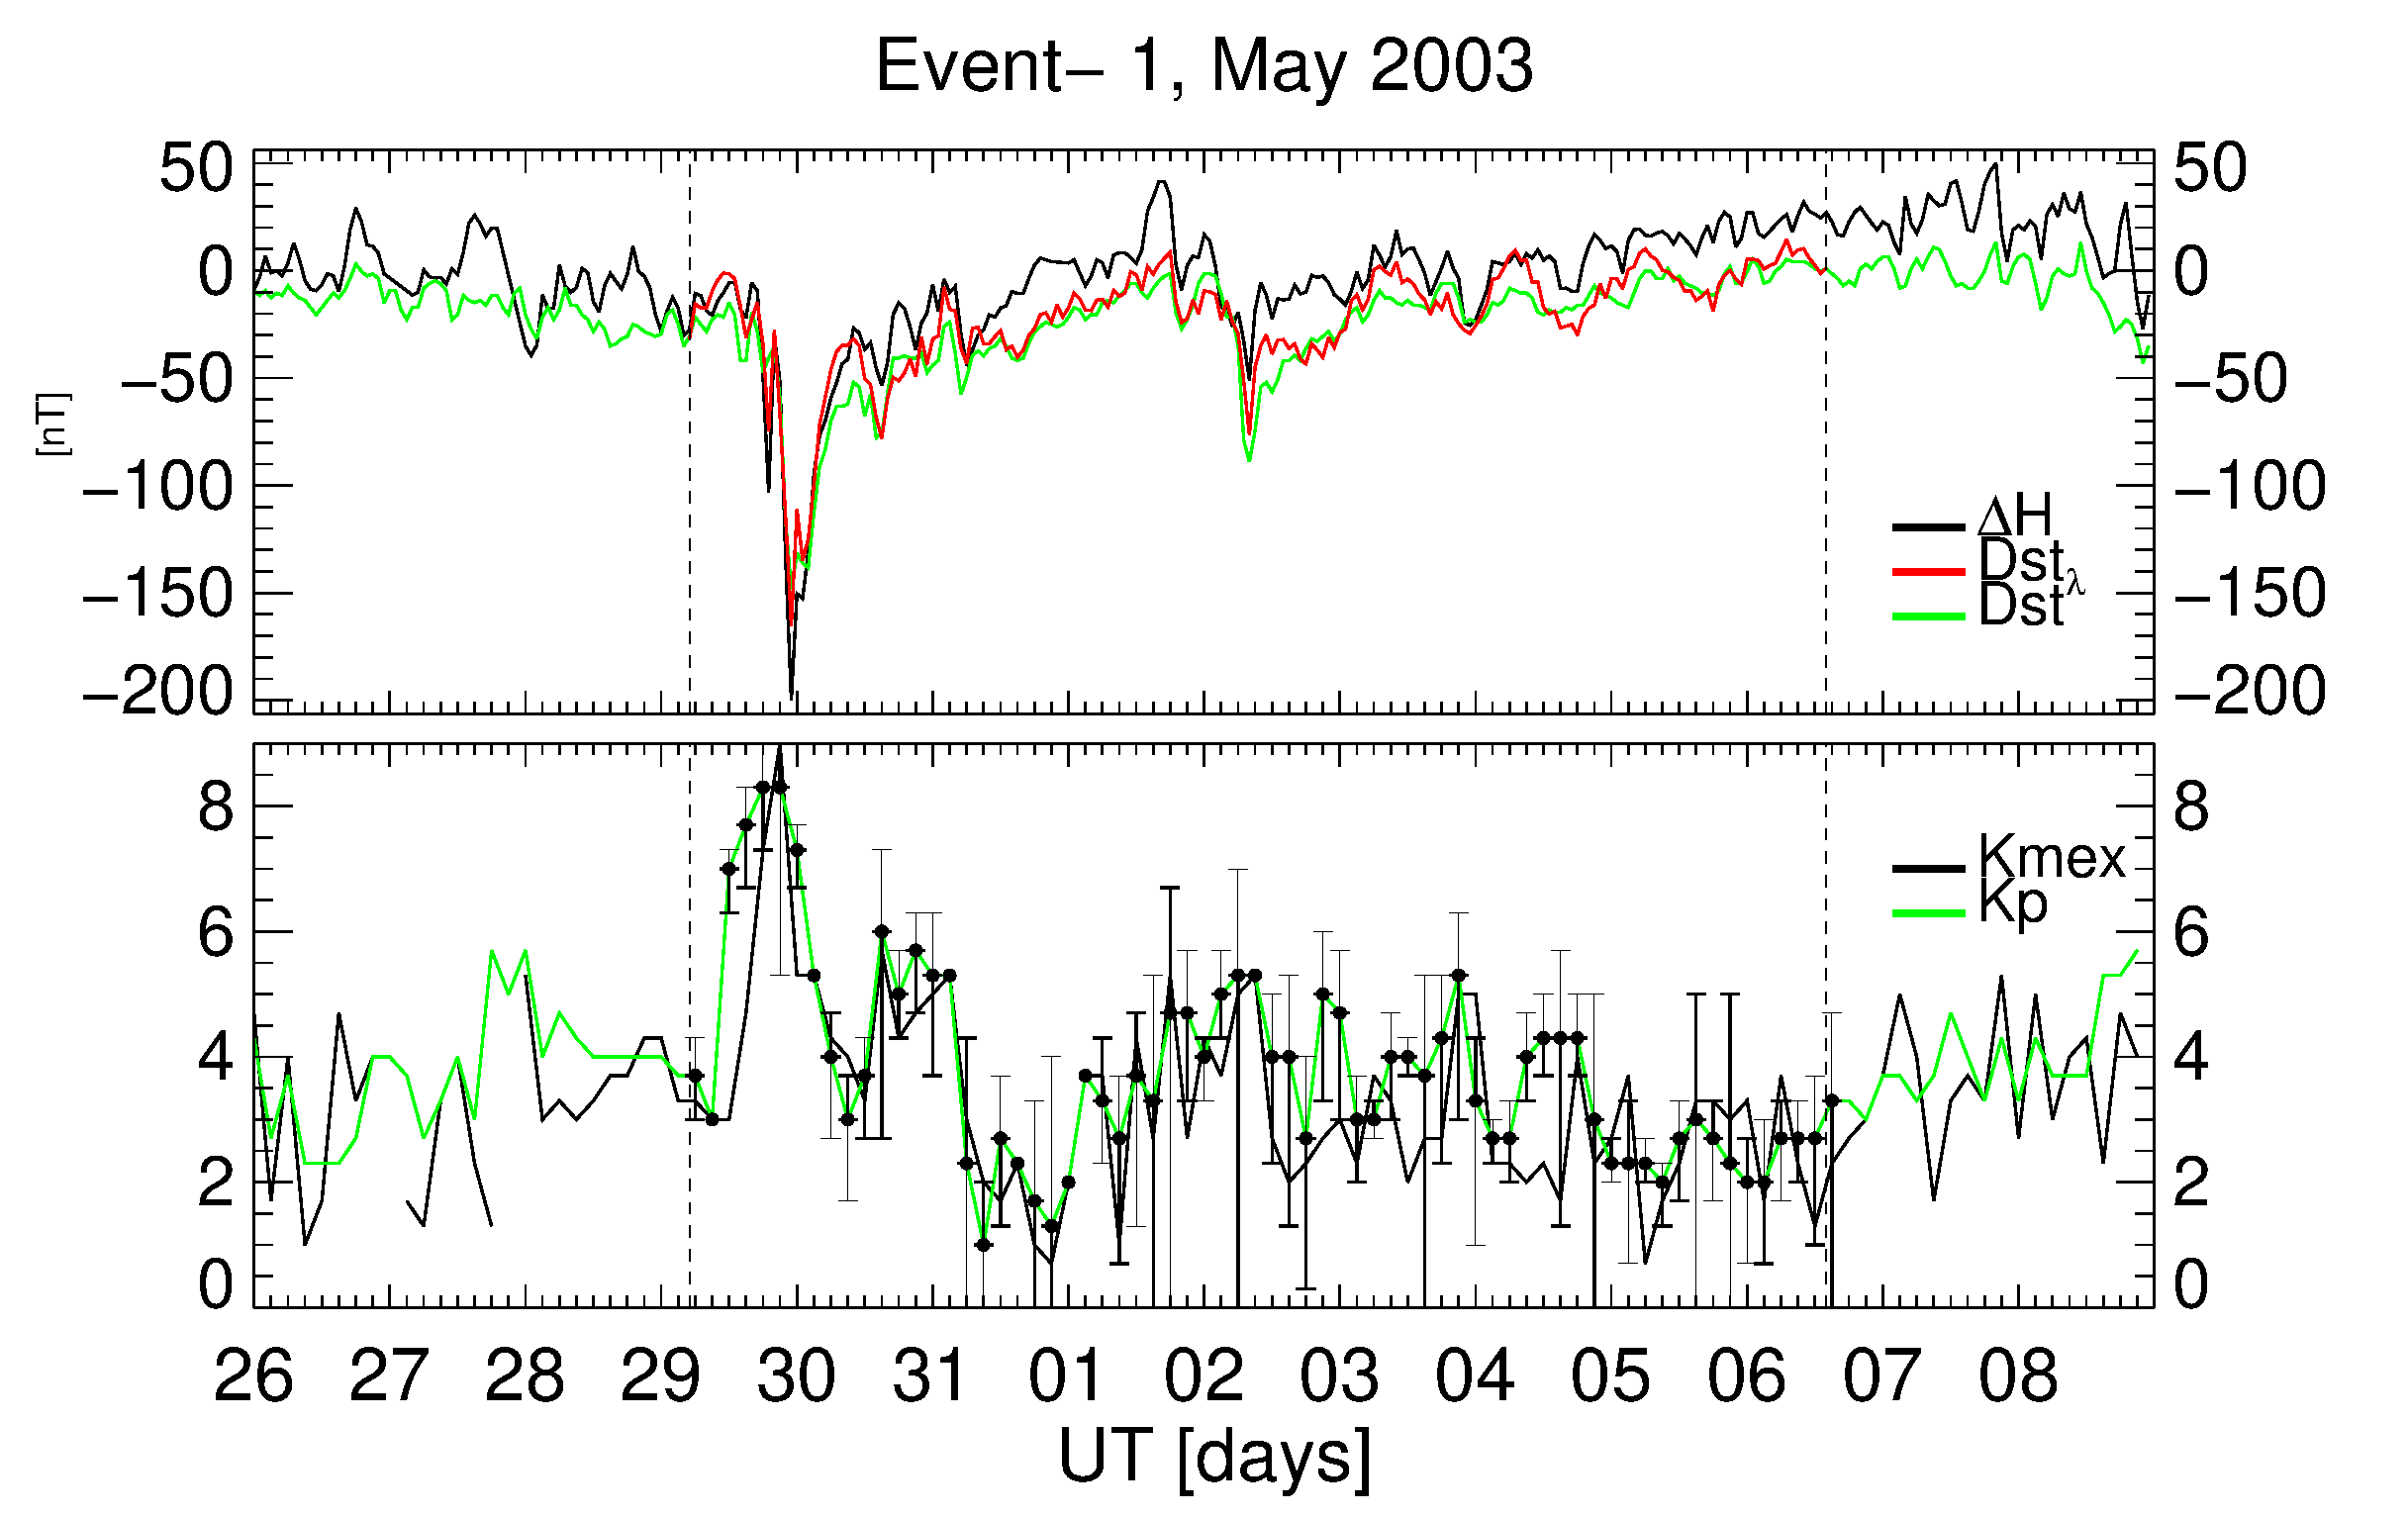
\includegraphics[width=6.0cm]{images/dH_approx/diono_valid_V4_2003-05-26.eps}
     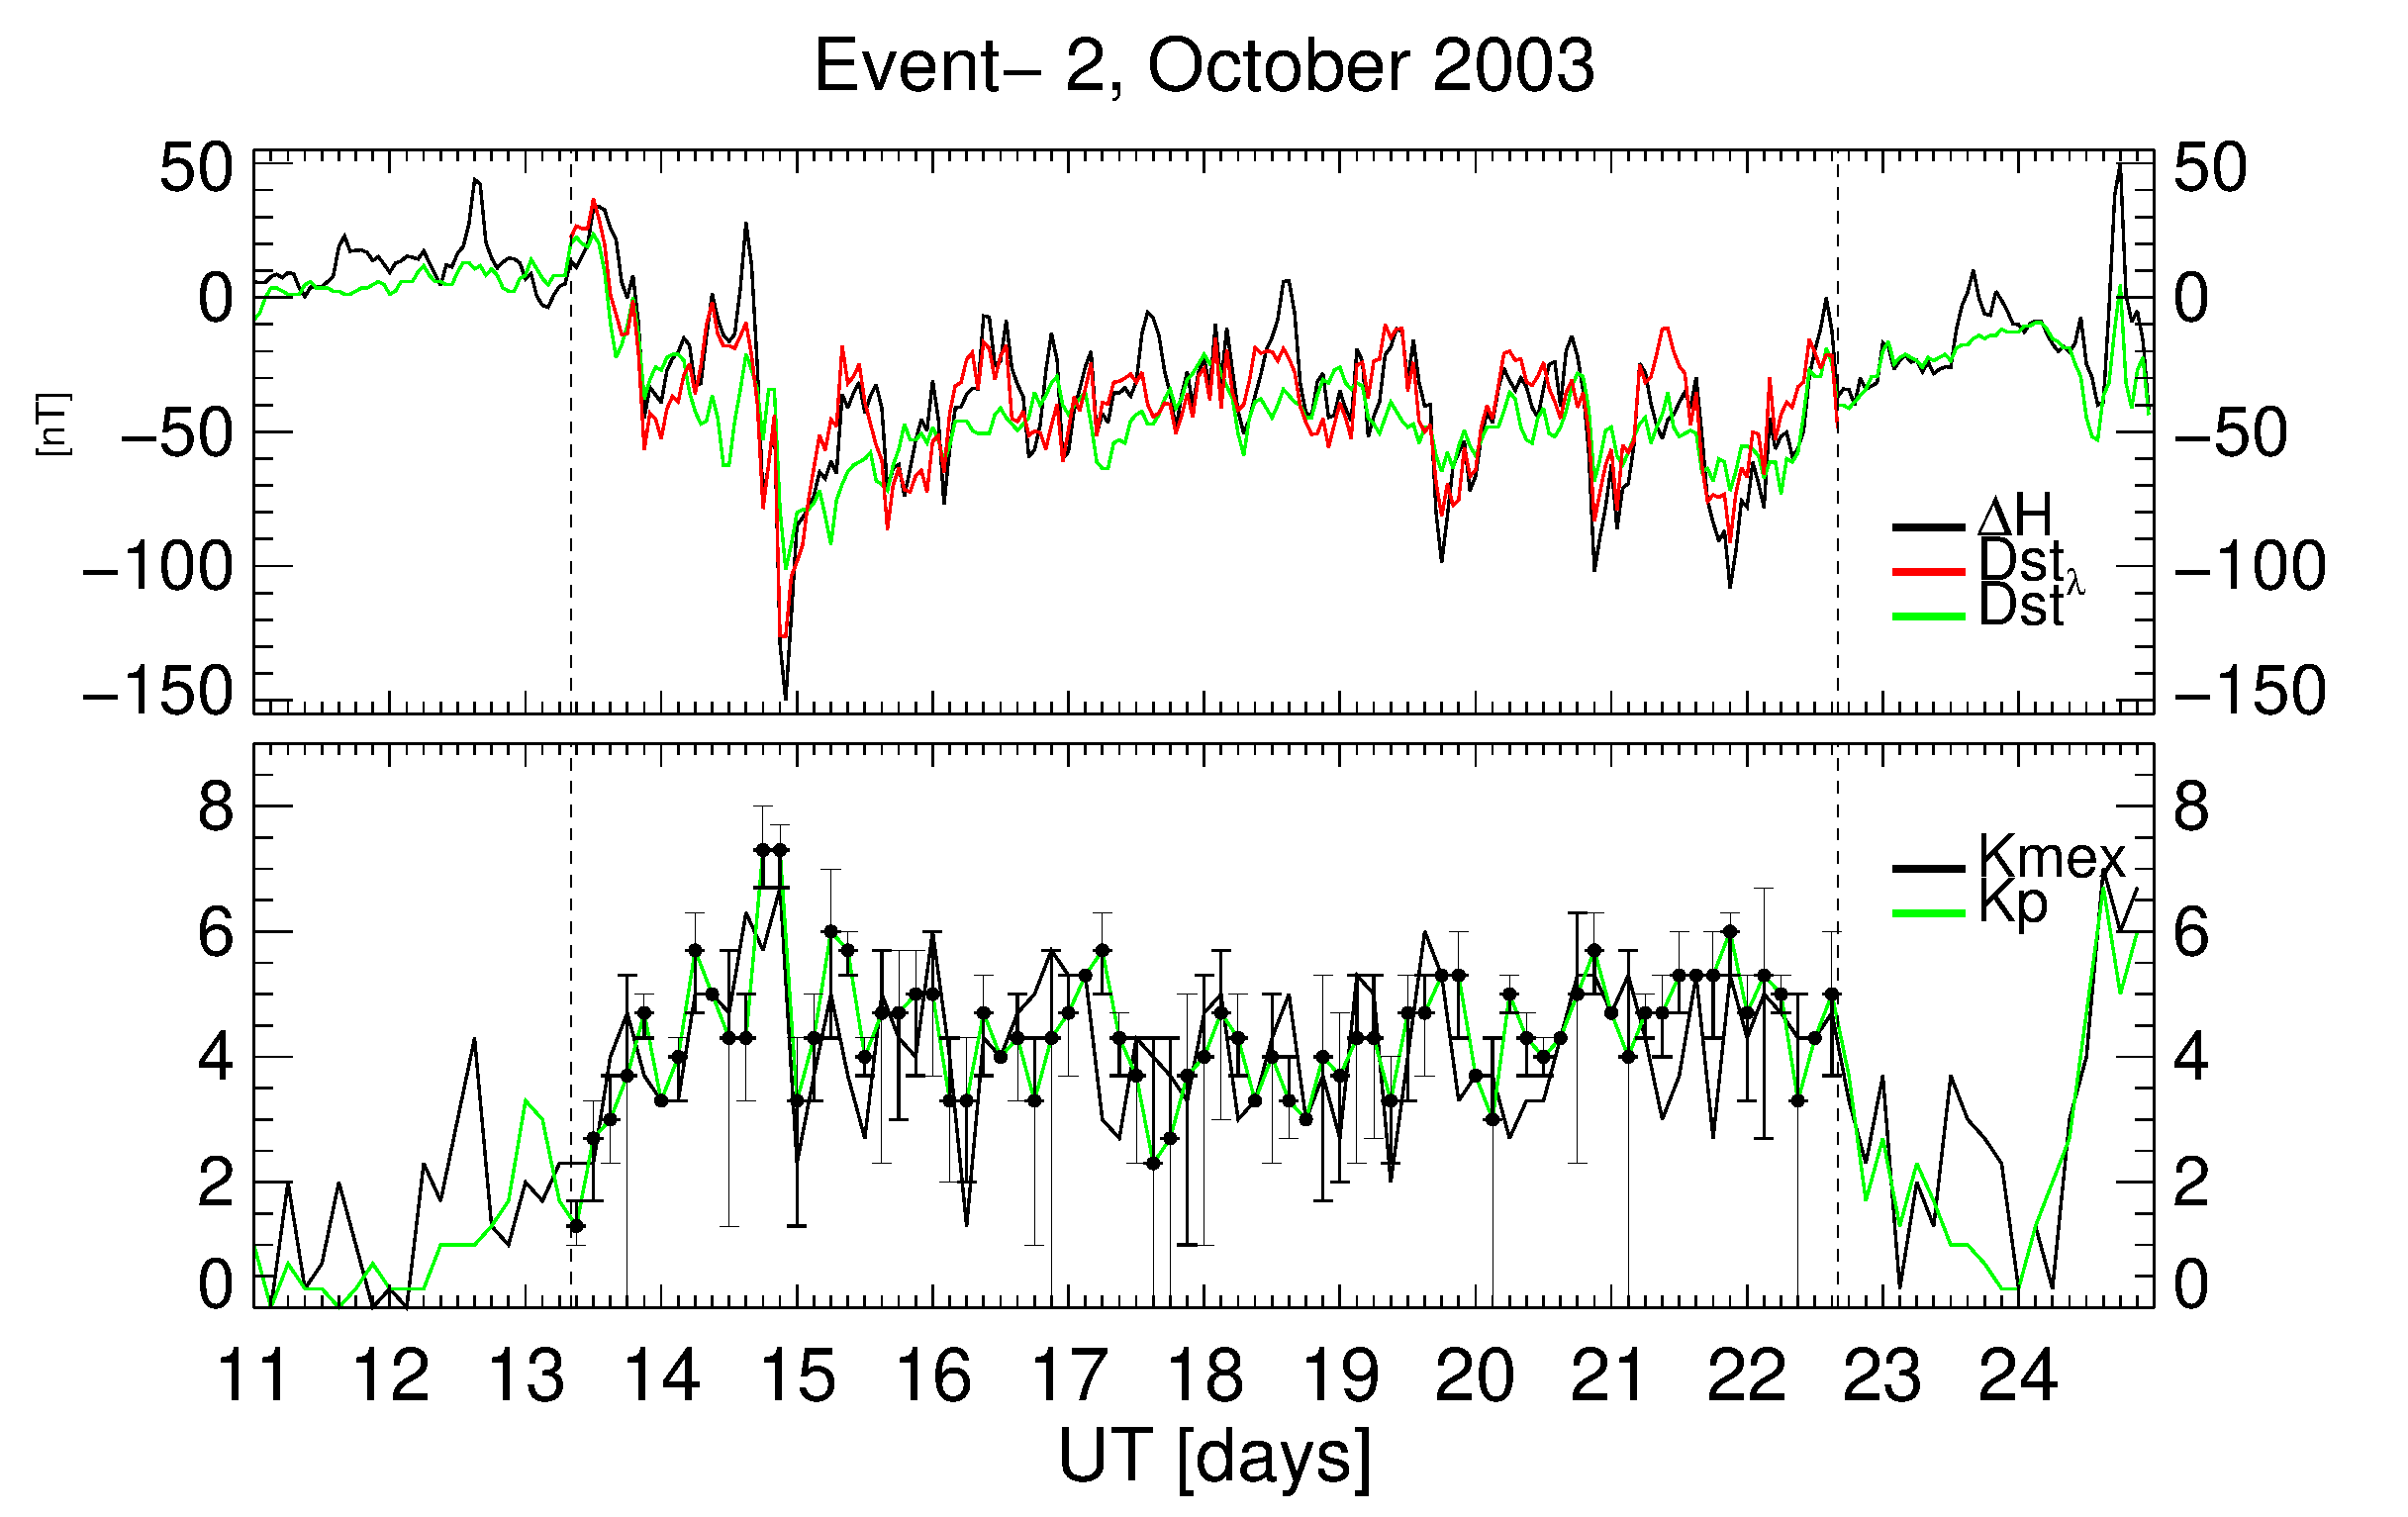
\includegraphics[width=6.0cm]{images/dH_approx/diono_valid_V4_2003-10-11.eps}
     \centerline{\Large \bf   
      \hspace{0.275\textwidth}  \color{black}{}
       \hspace{0.295\textwidth}  \color{black}{}
         \hfill}
     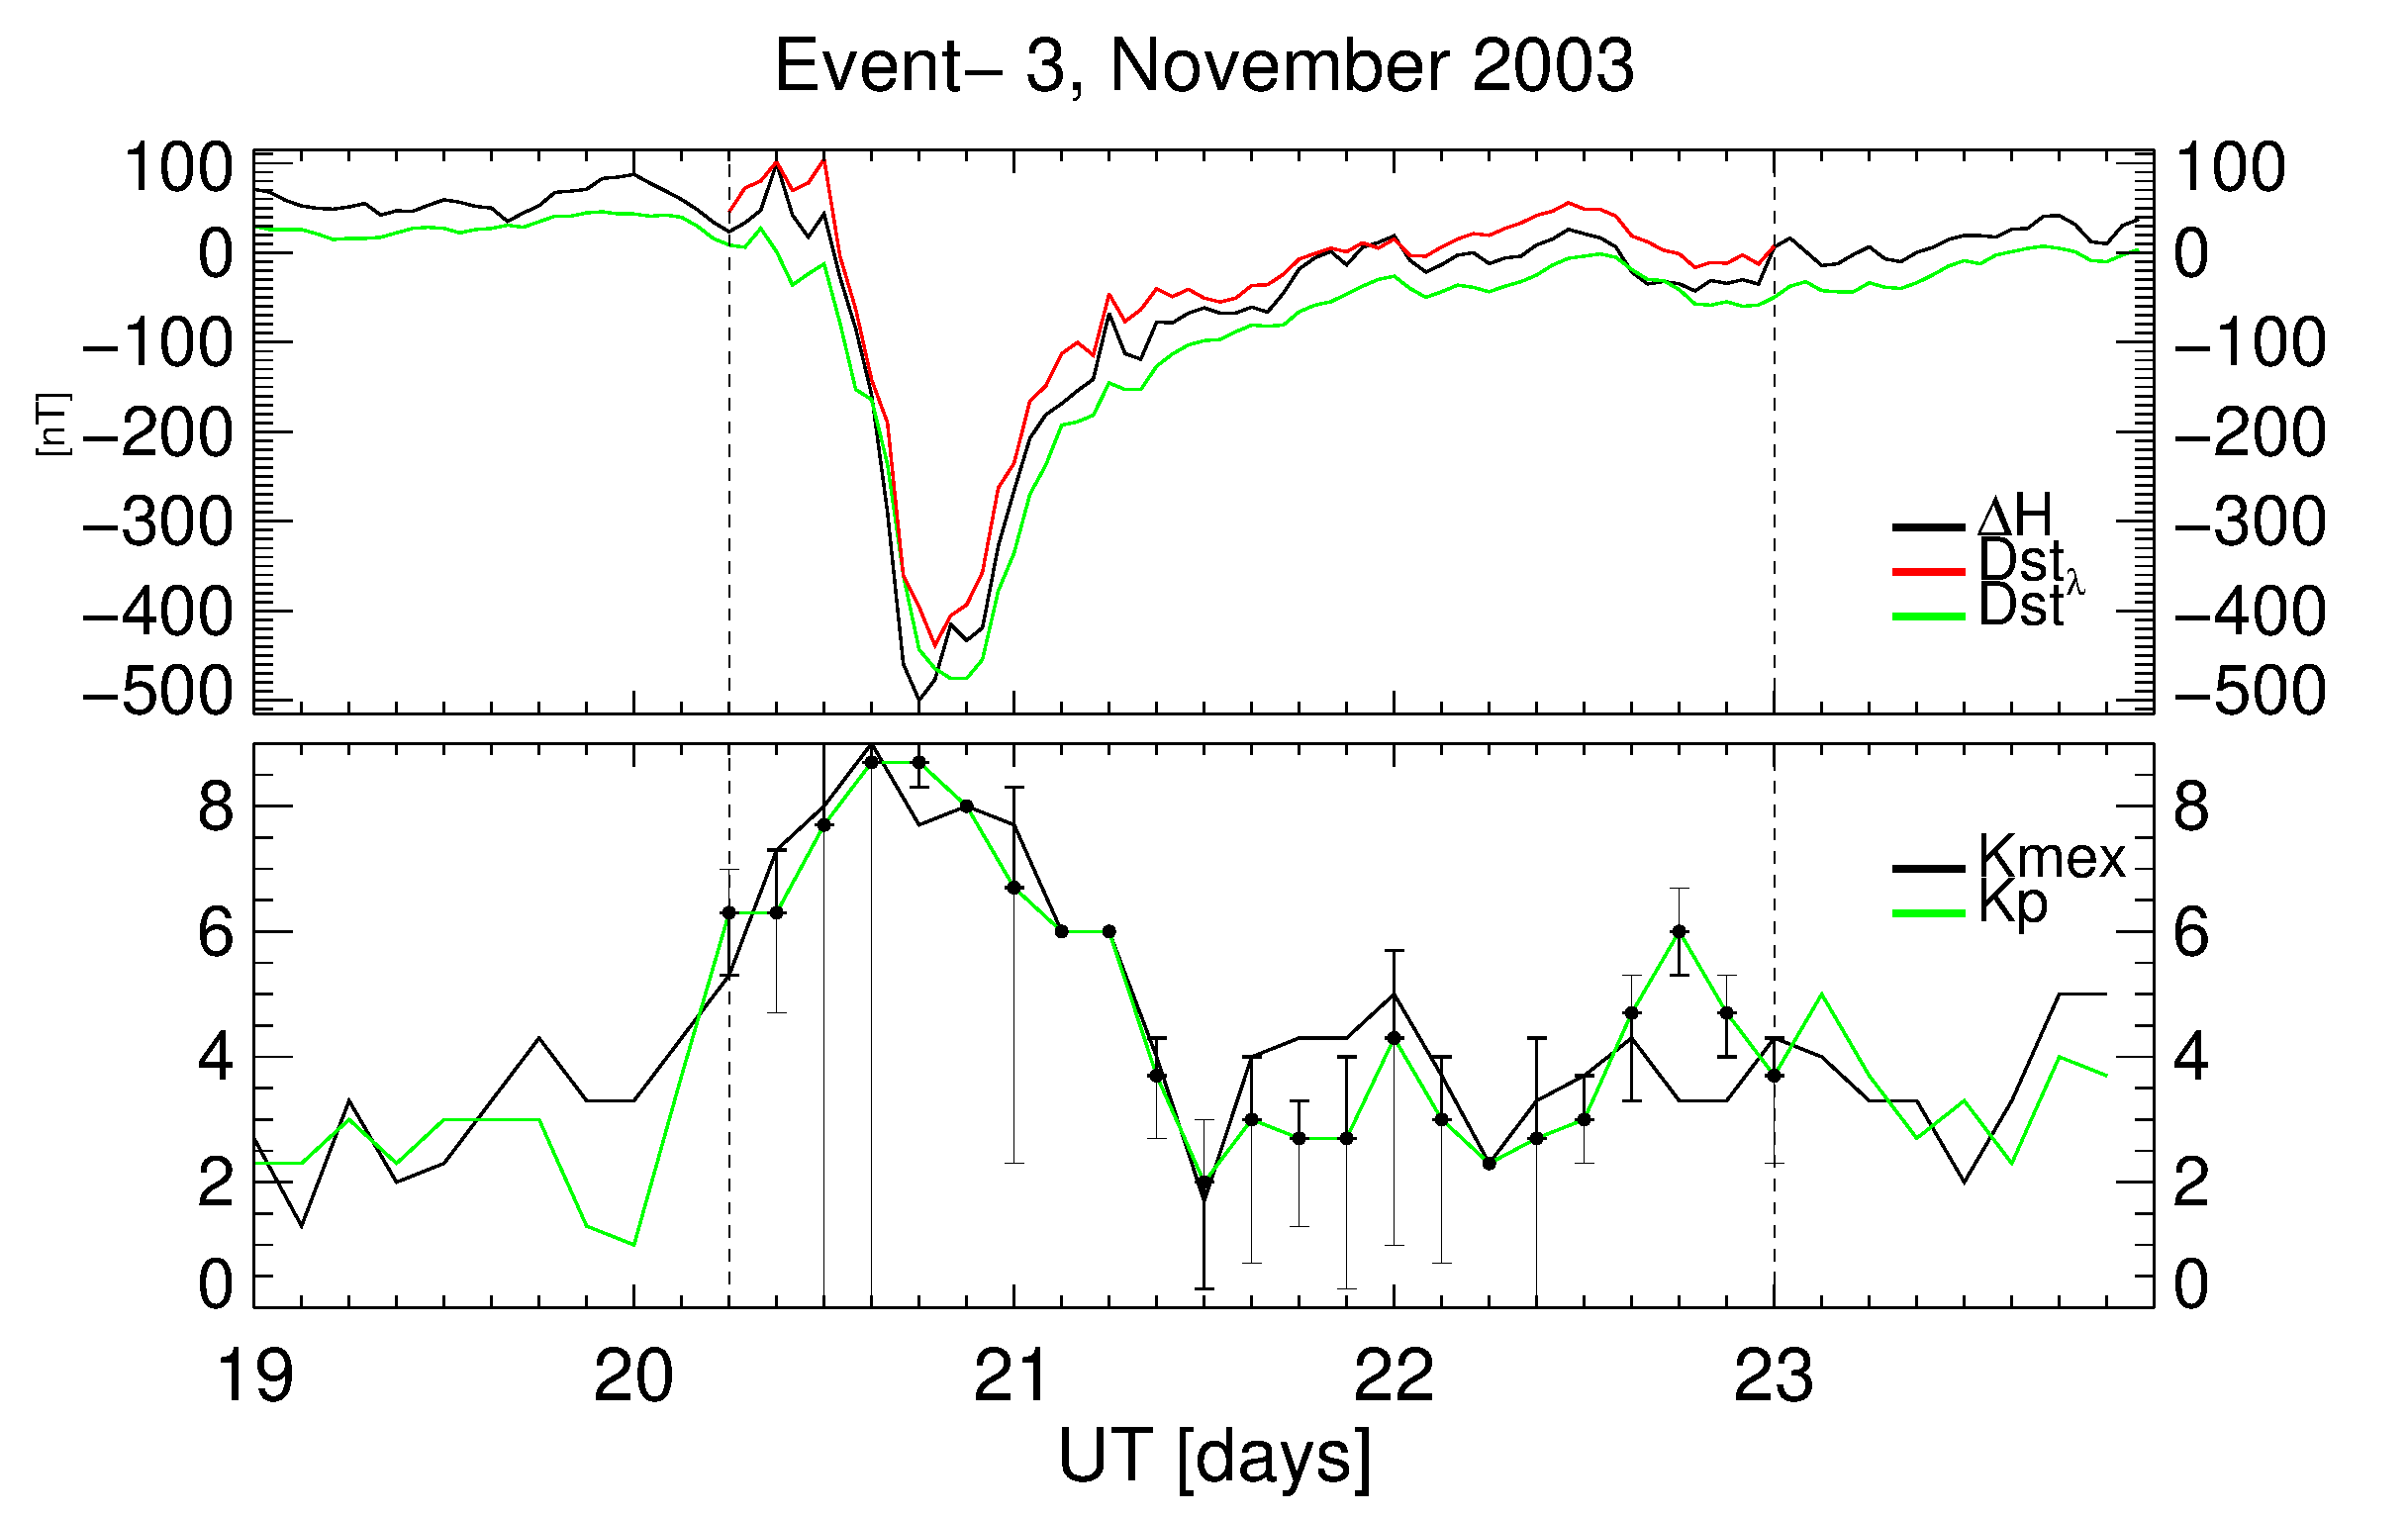
\includegraphics[width=6.0cm]{images/dH_approx/diono_valid_V4_2003-11-19.eps}     
     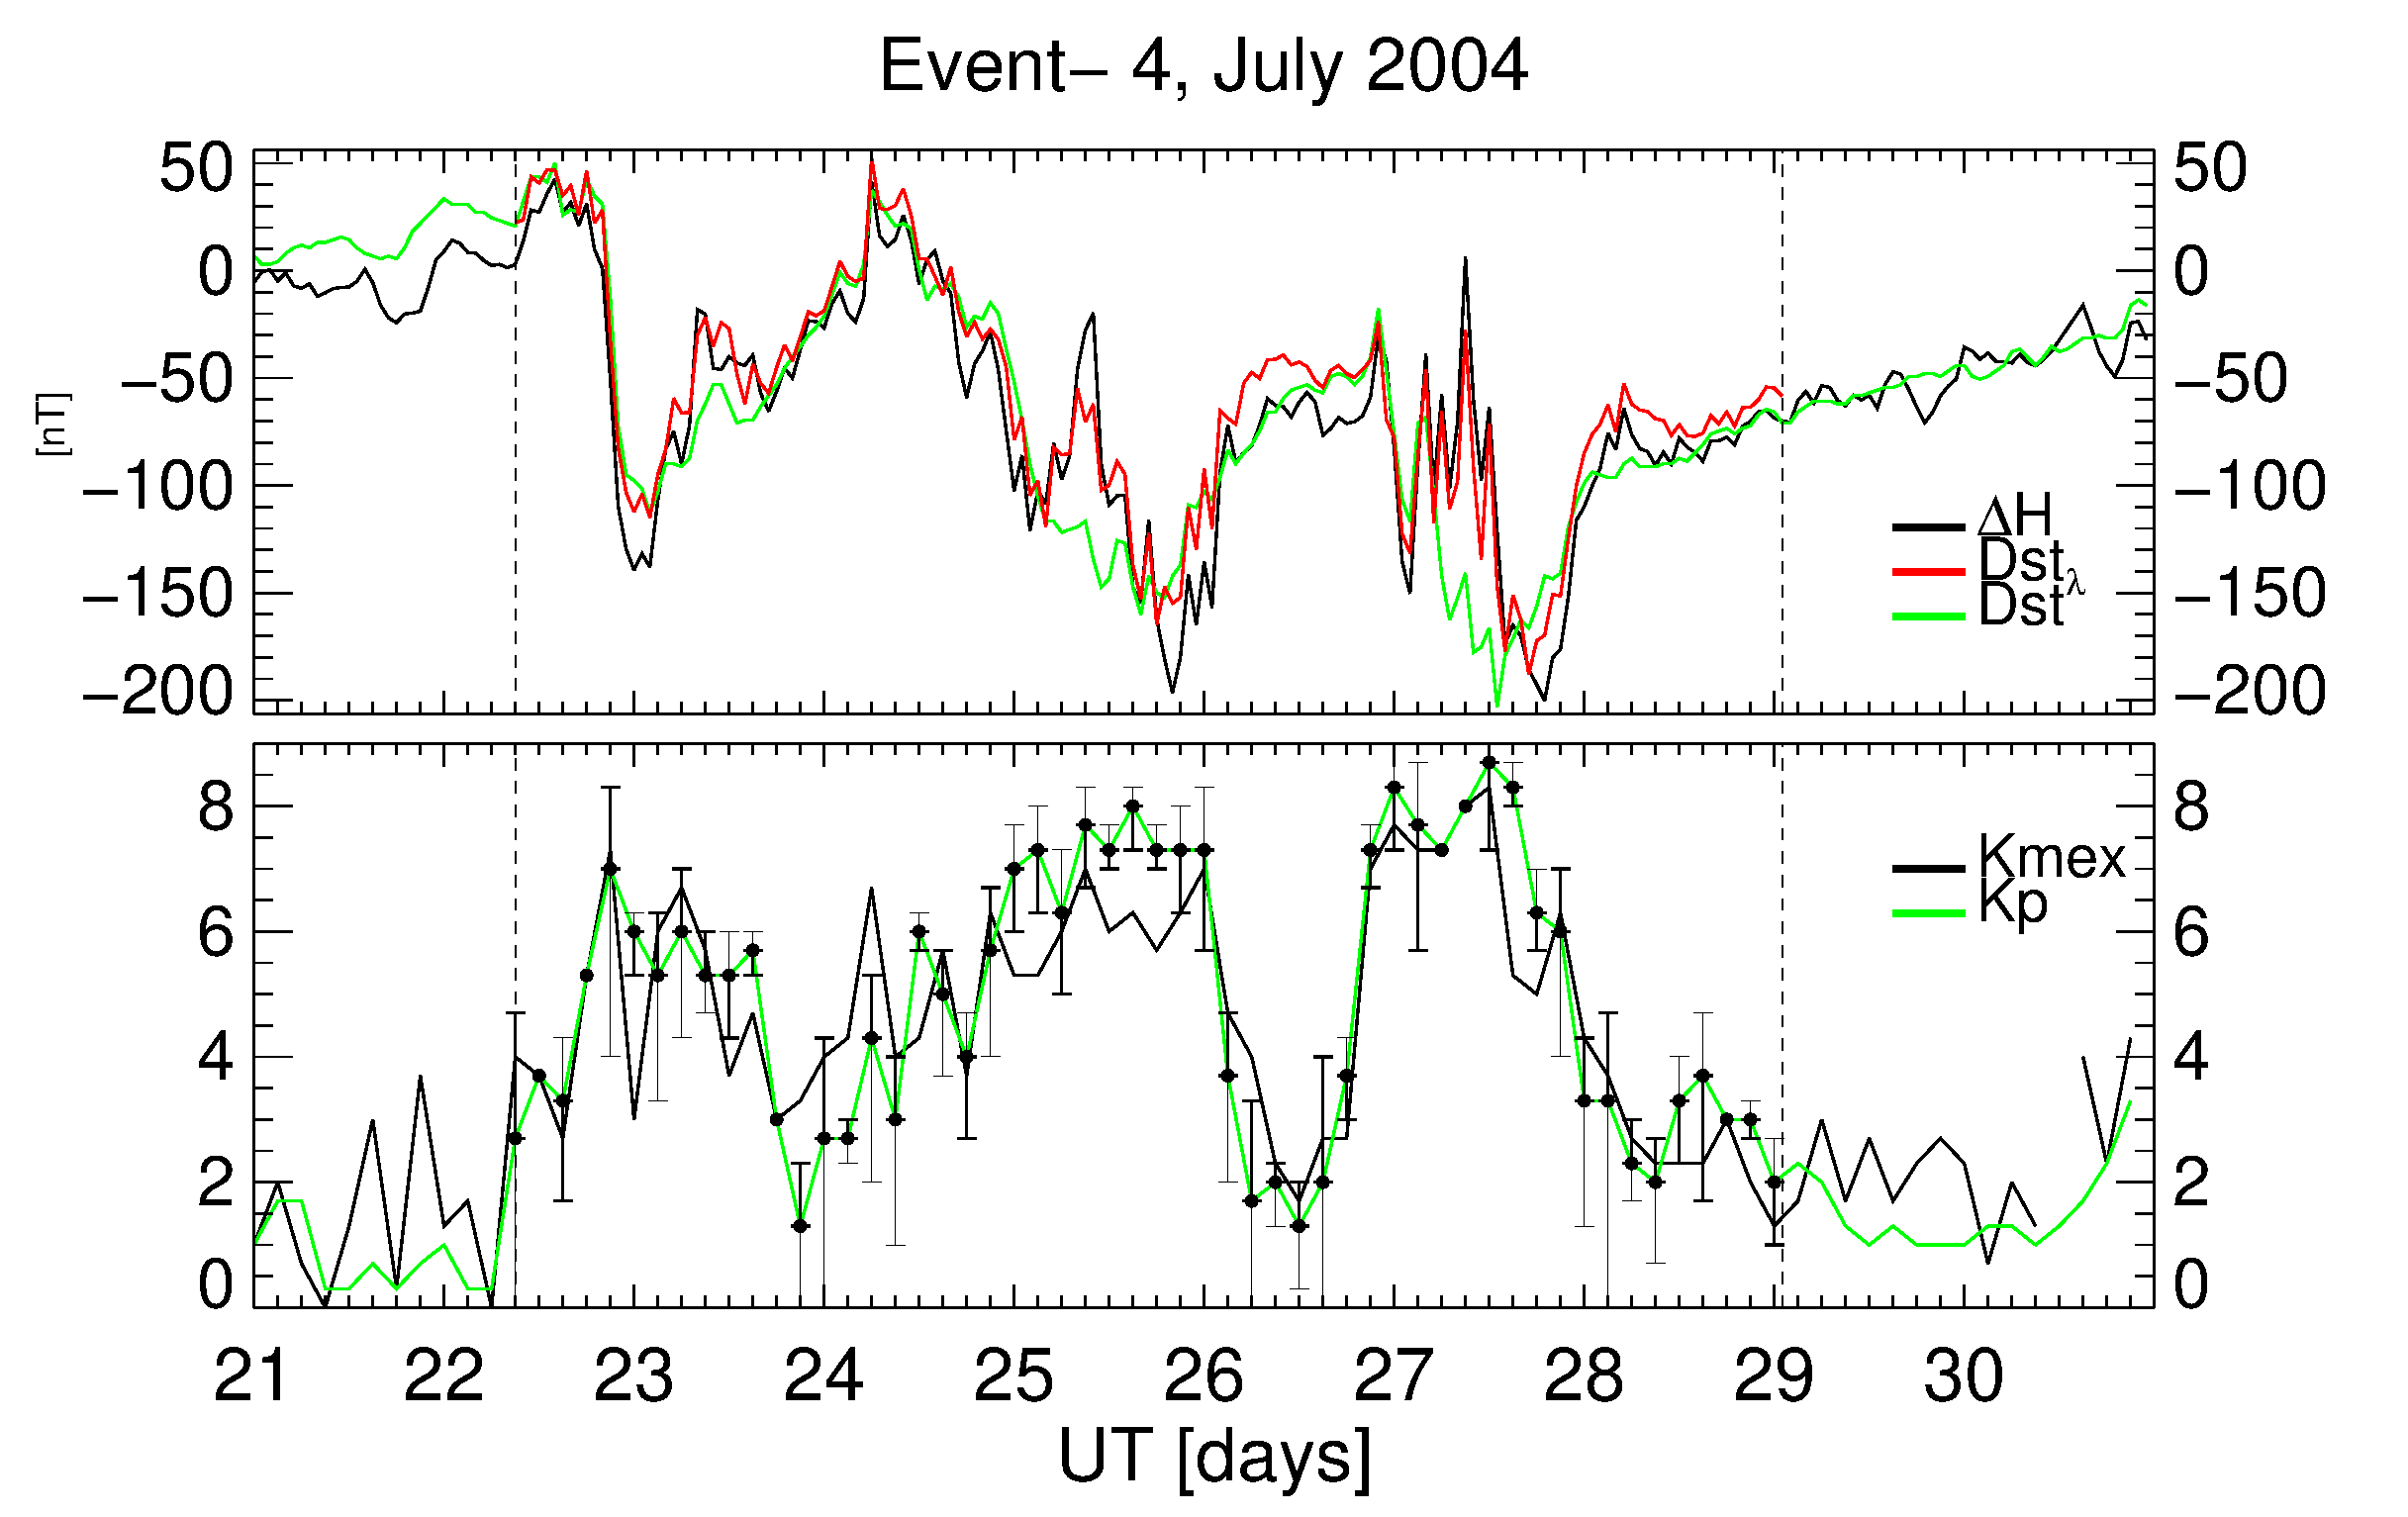
\includegraphics[width=6.0cm]{images/dH_approx/diono_valid_V4_2004-07-21.eps}
     \centerline{\Large \bf   
      \hspace{0.275\textwidth}  \color{black}{}
       \hspace{0.295\textwidth}  \color{black}{}
         \hfill}
      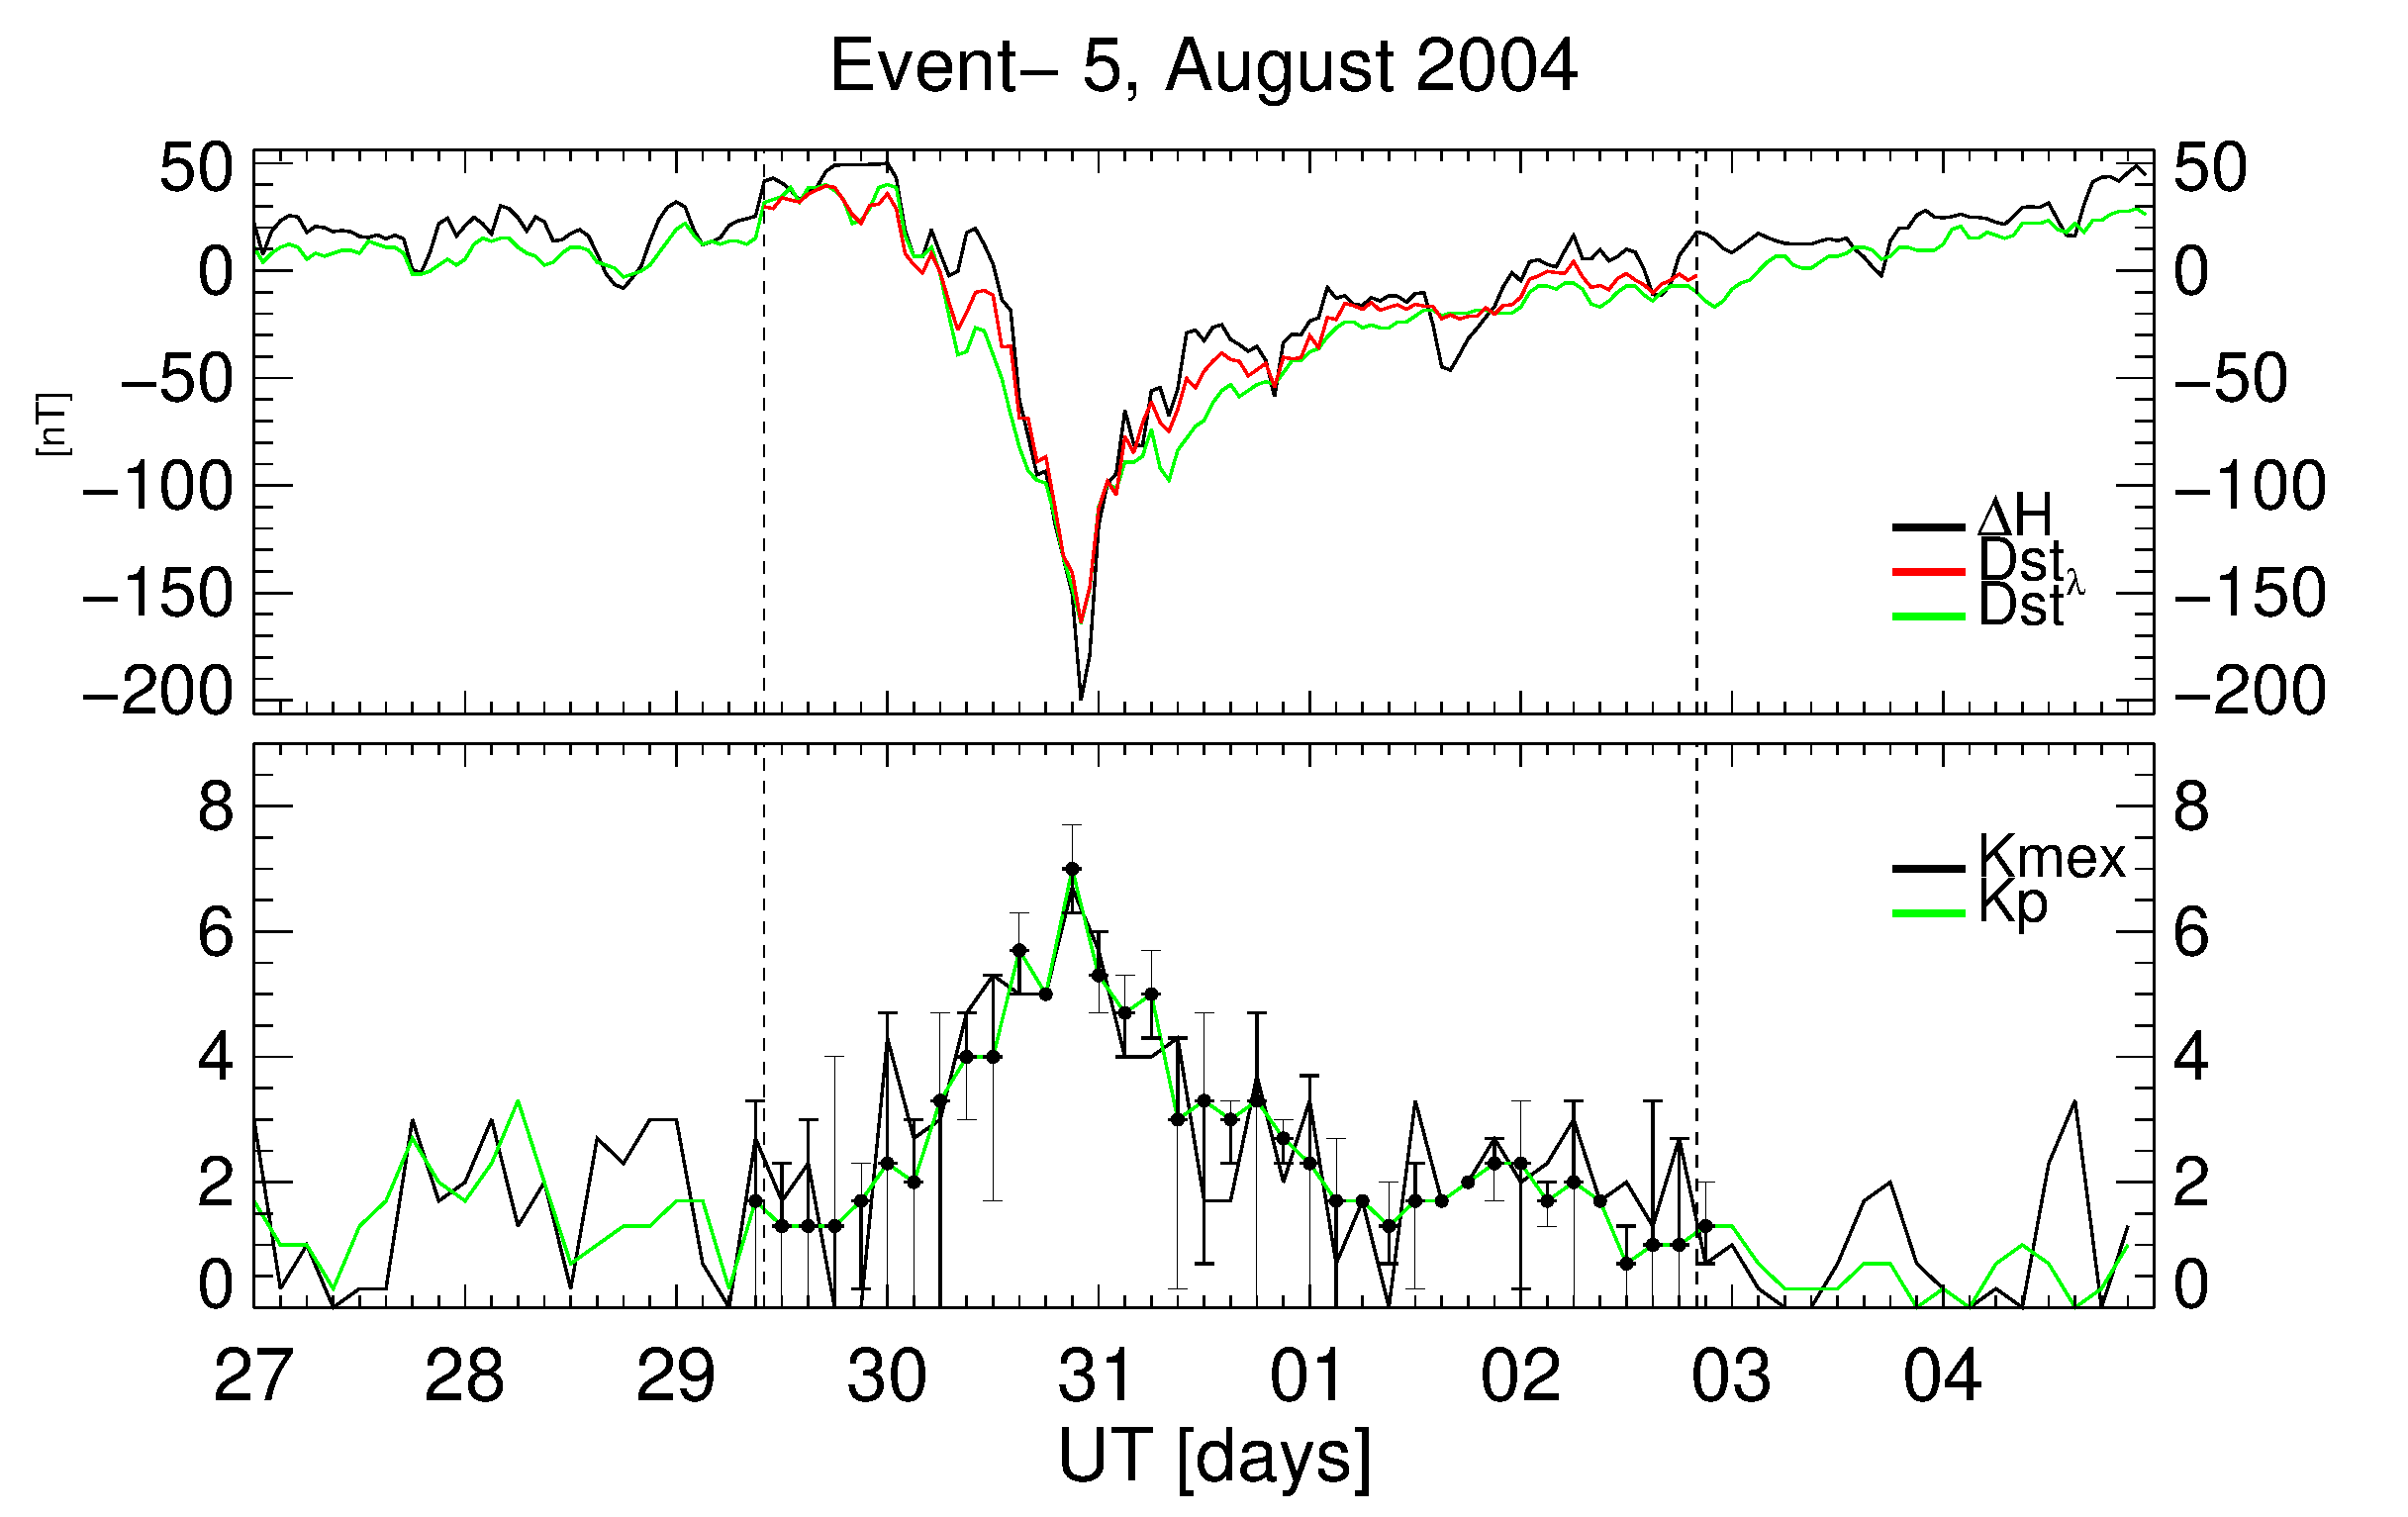
\includegraphics[width=6.0cm]{images/dH_approx/diono_valid_V4_2004-08-27.eps}     
      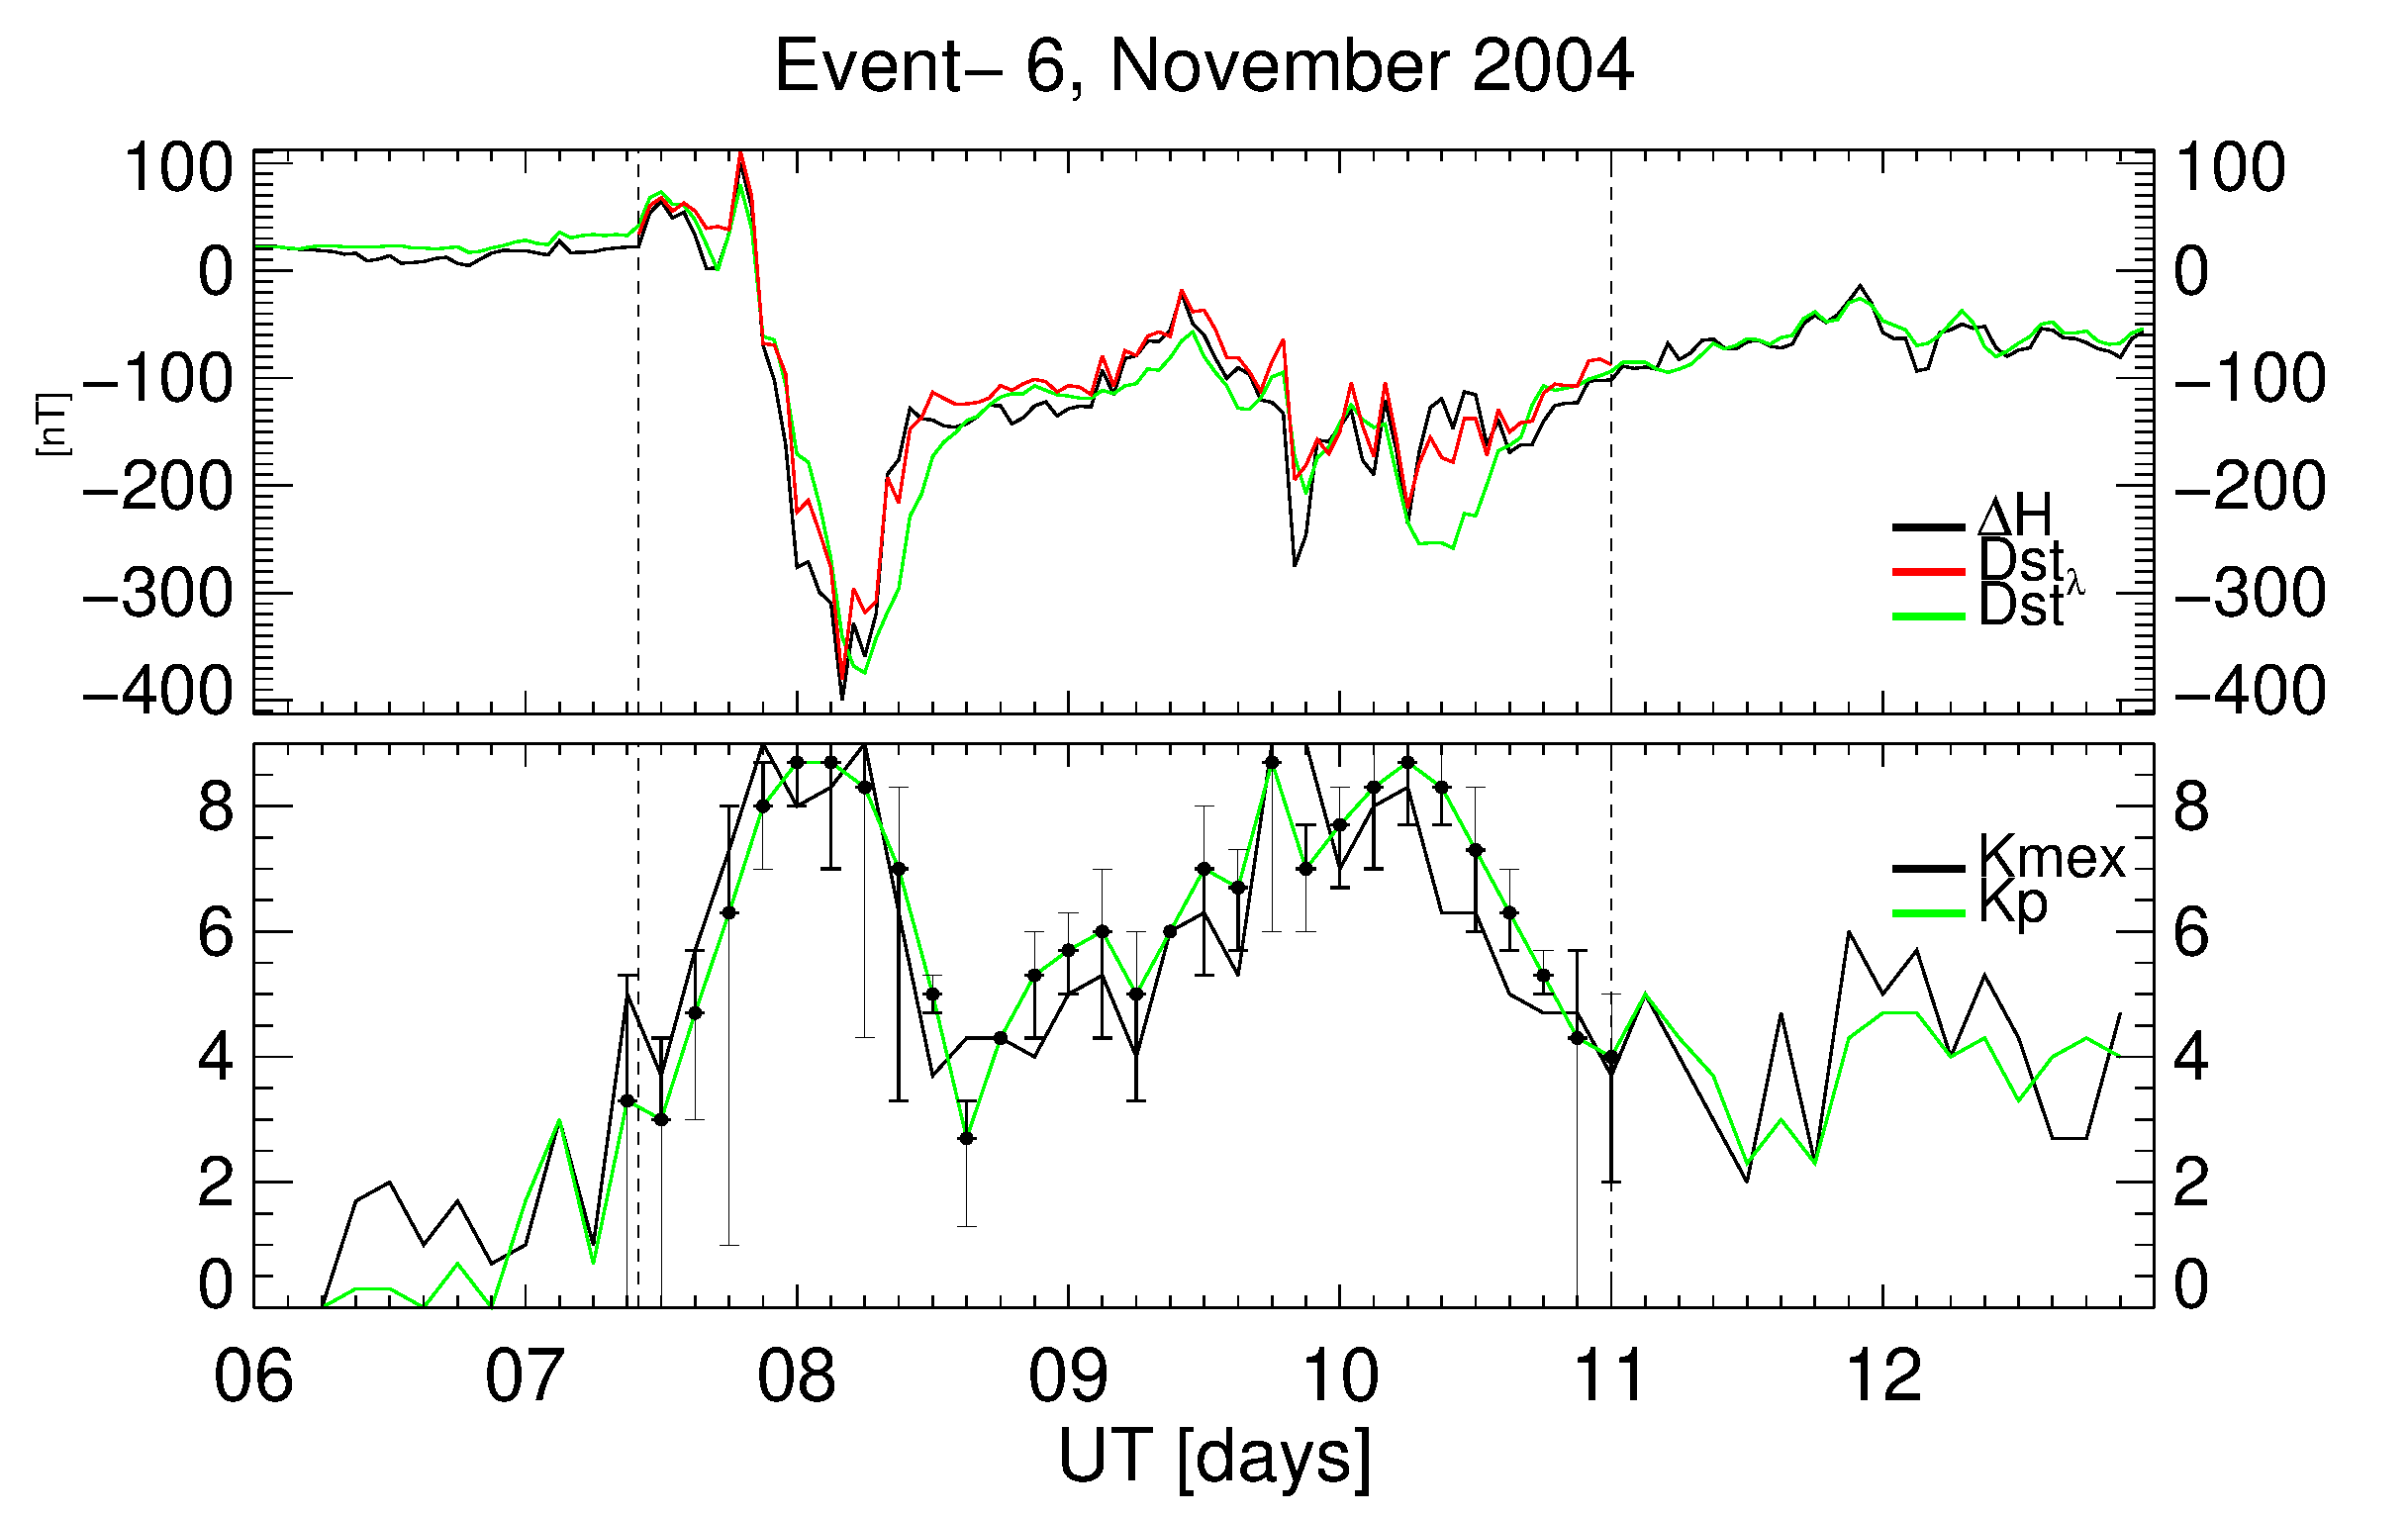
\includegraphics[width=6.0cm]{images/dH_approx/diono_valid_V4_2004-11-06.eps}
       \centerline{\Large \bf   
      \hspace{0.275\textwidth}  \color{black}{}
       \hspace{0.295\textwidth}  \color{black}{}
         \hfill}
       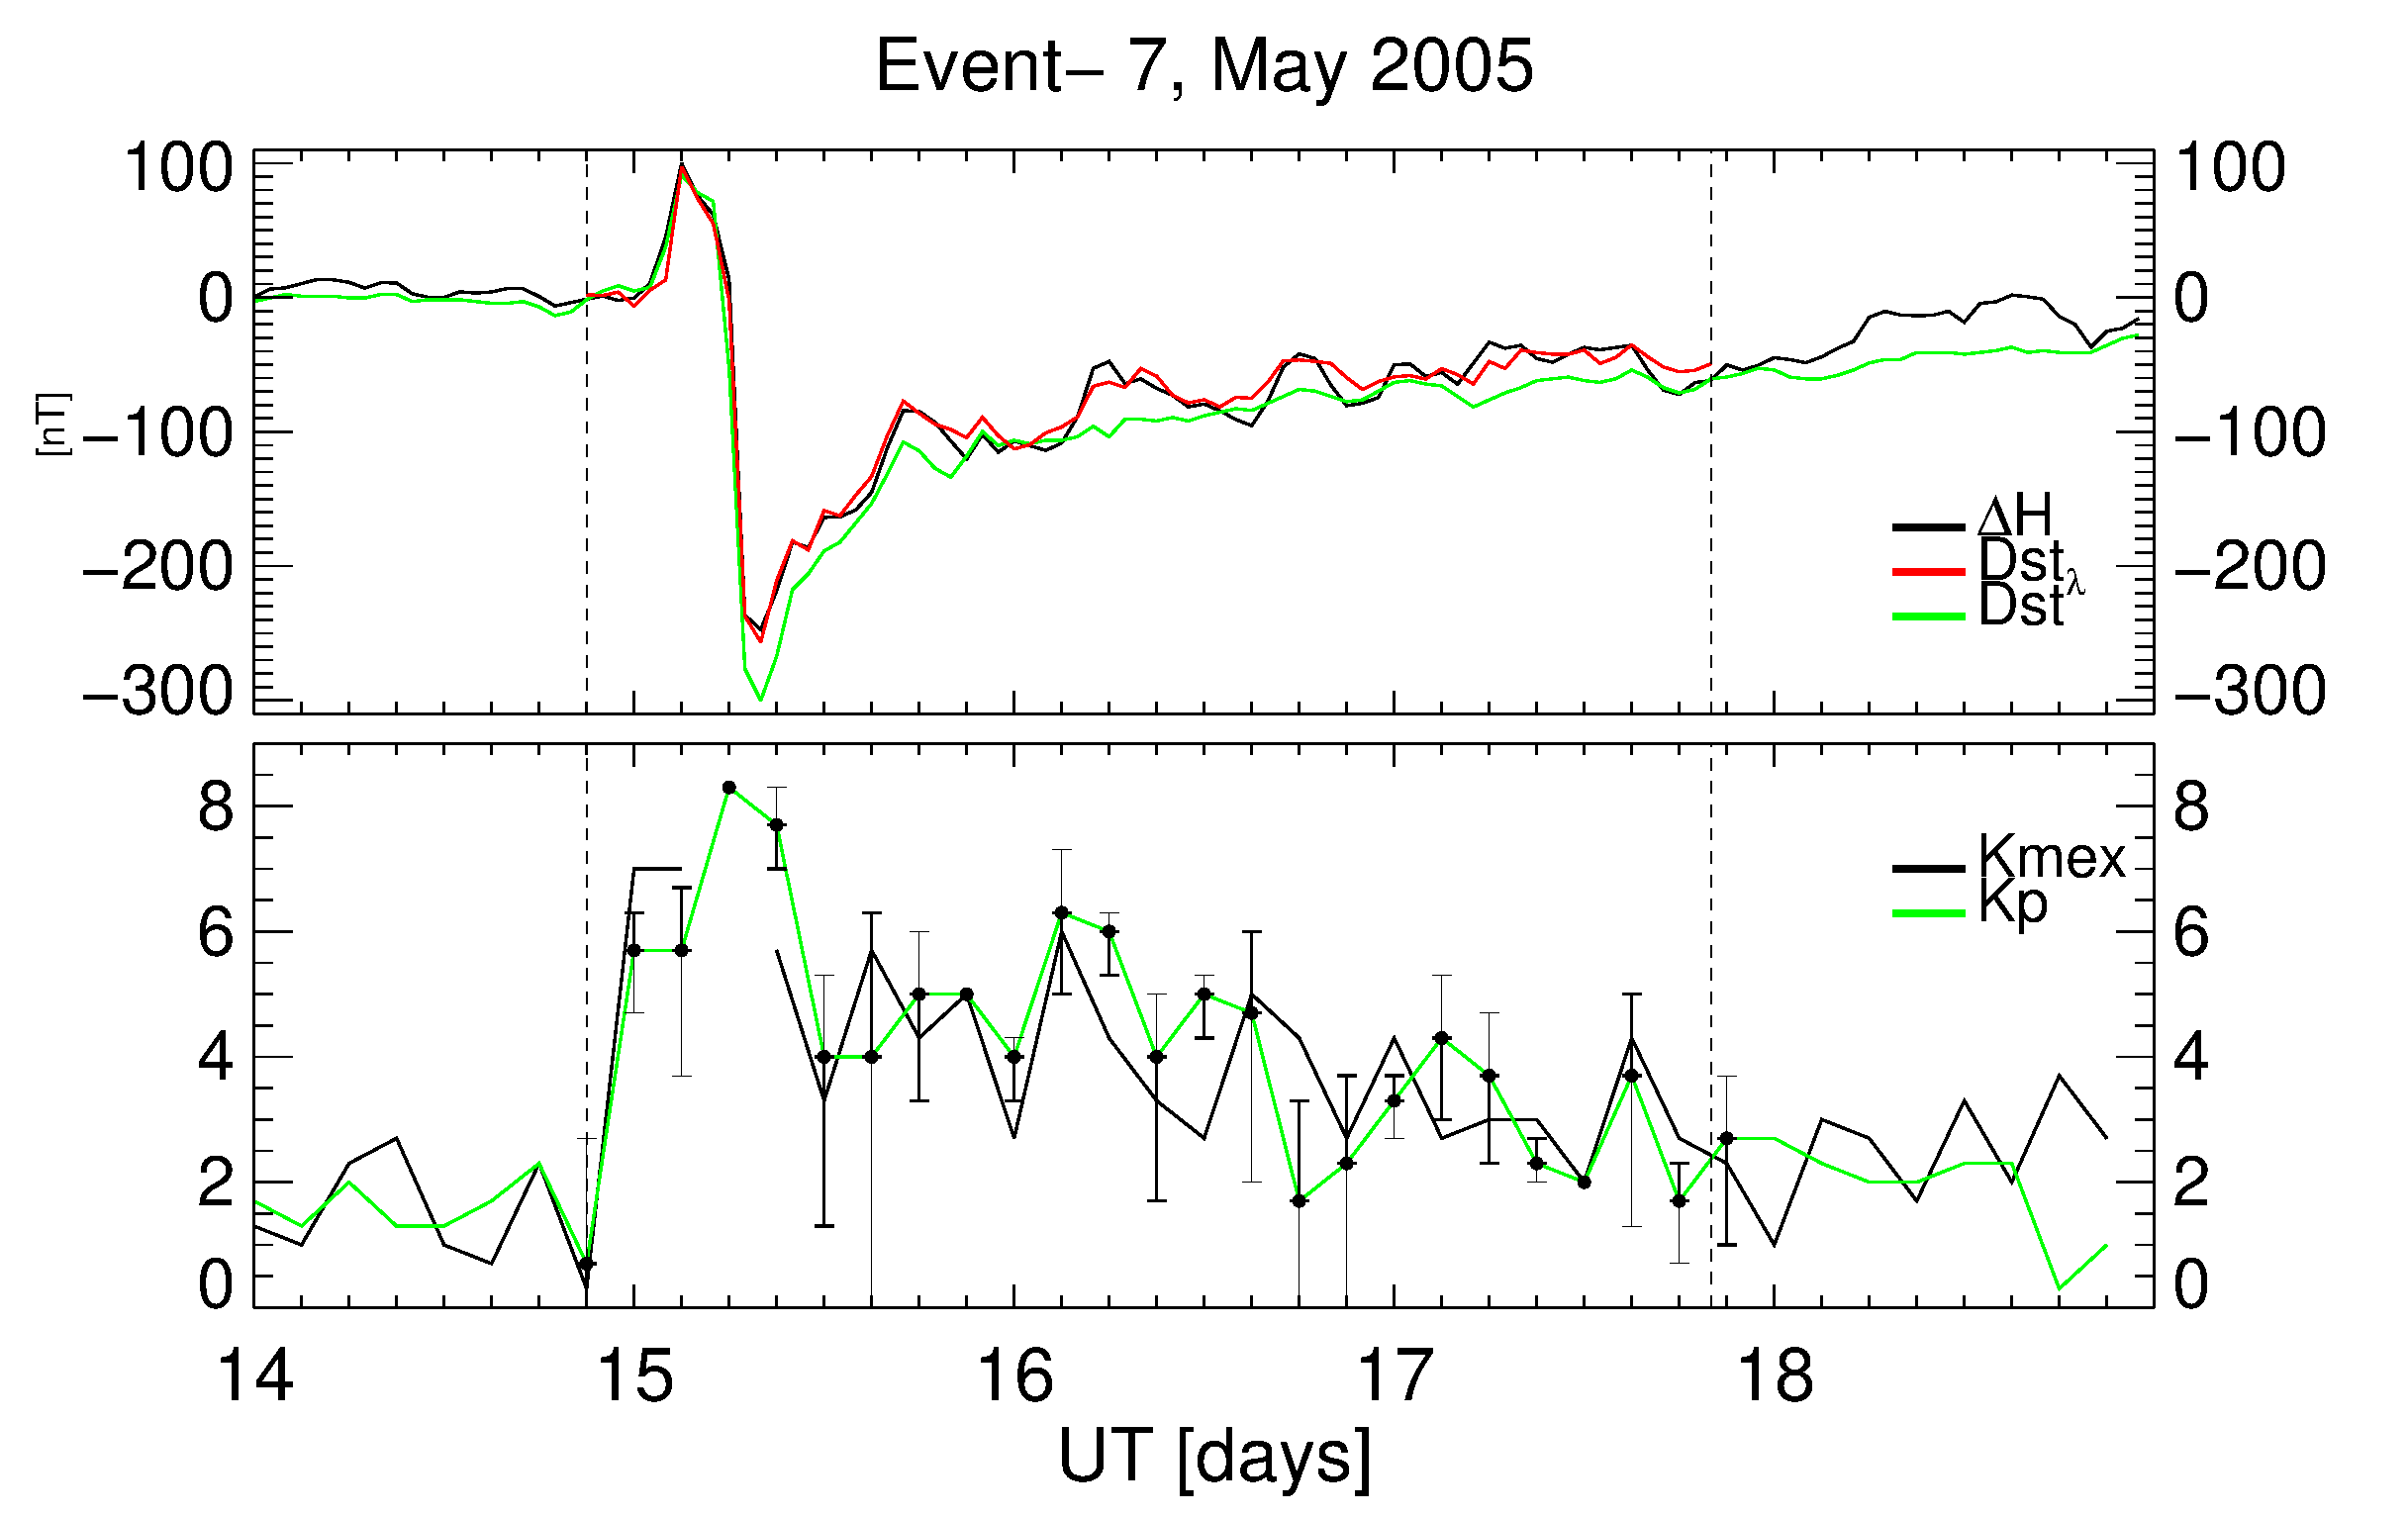
\includegraphics[width=6.0cm]{images/dH_approx/diono_valid_V4_2005-05-14.eps}     
       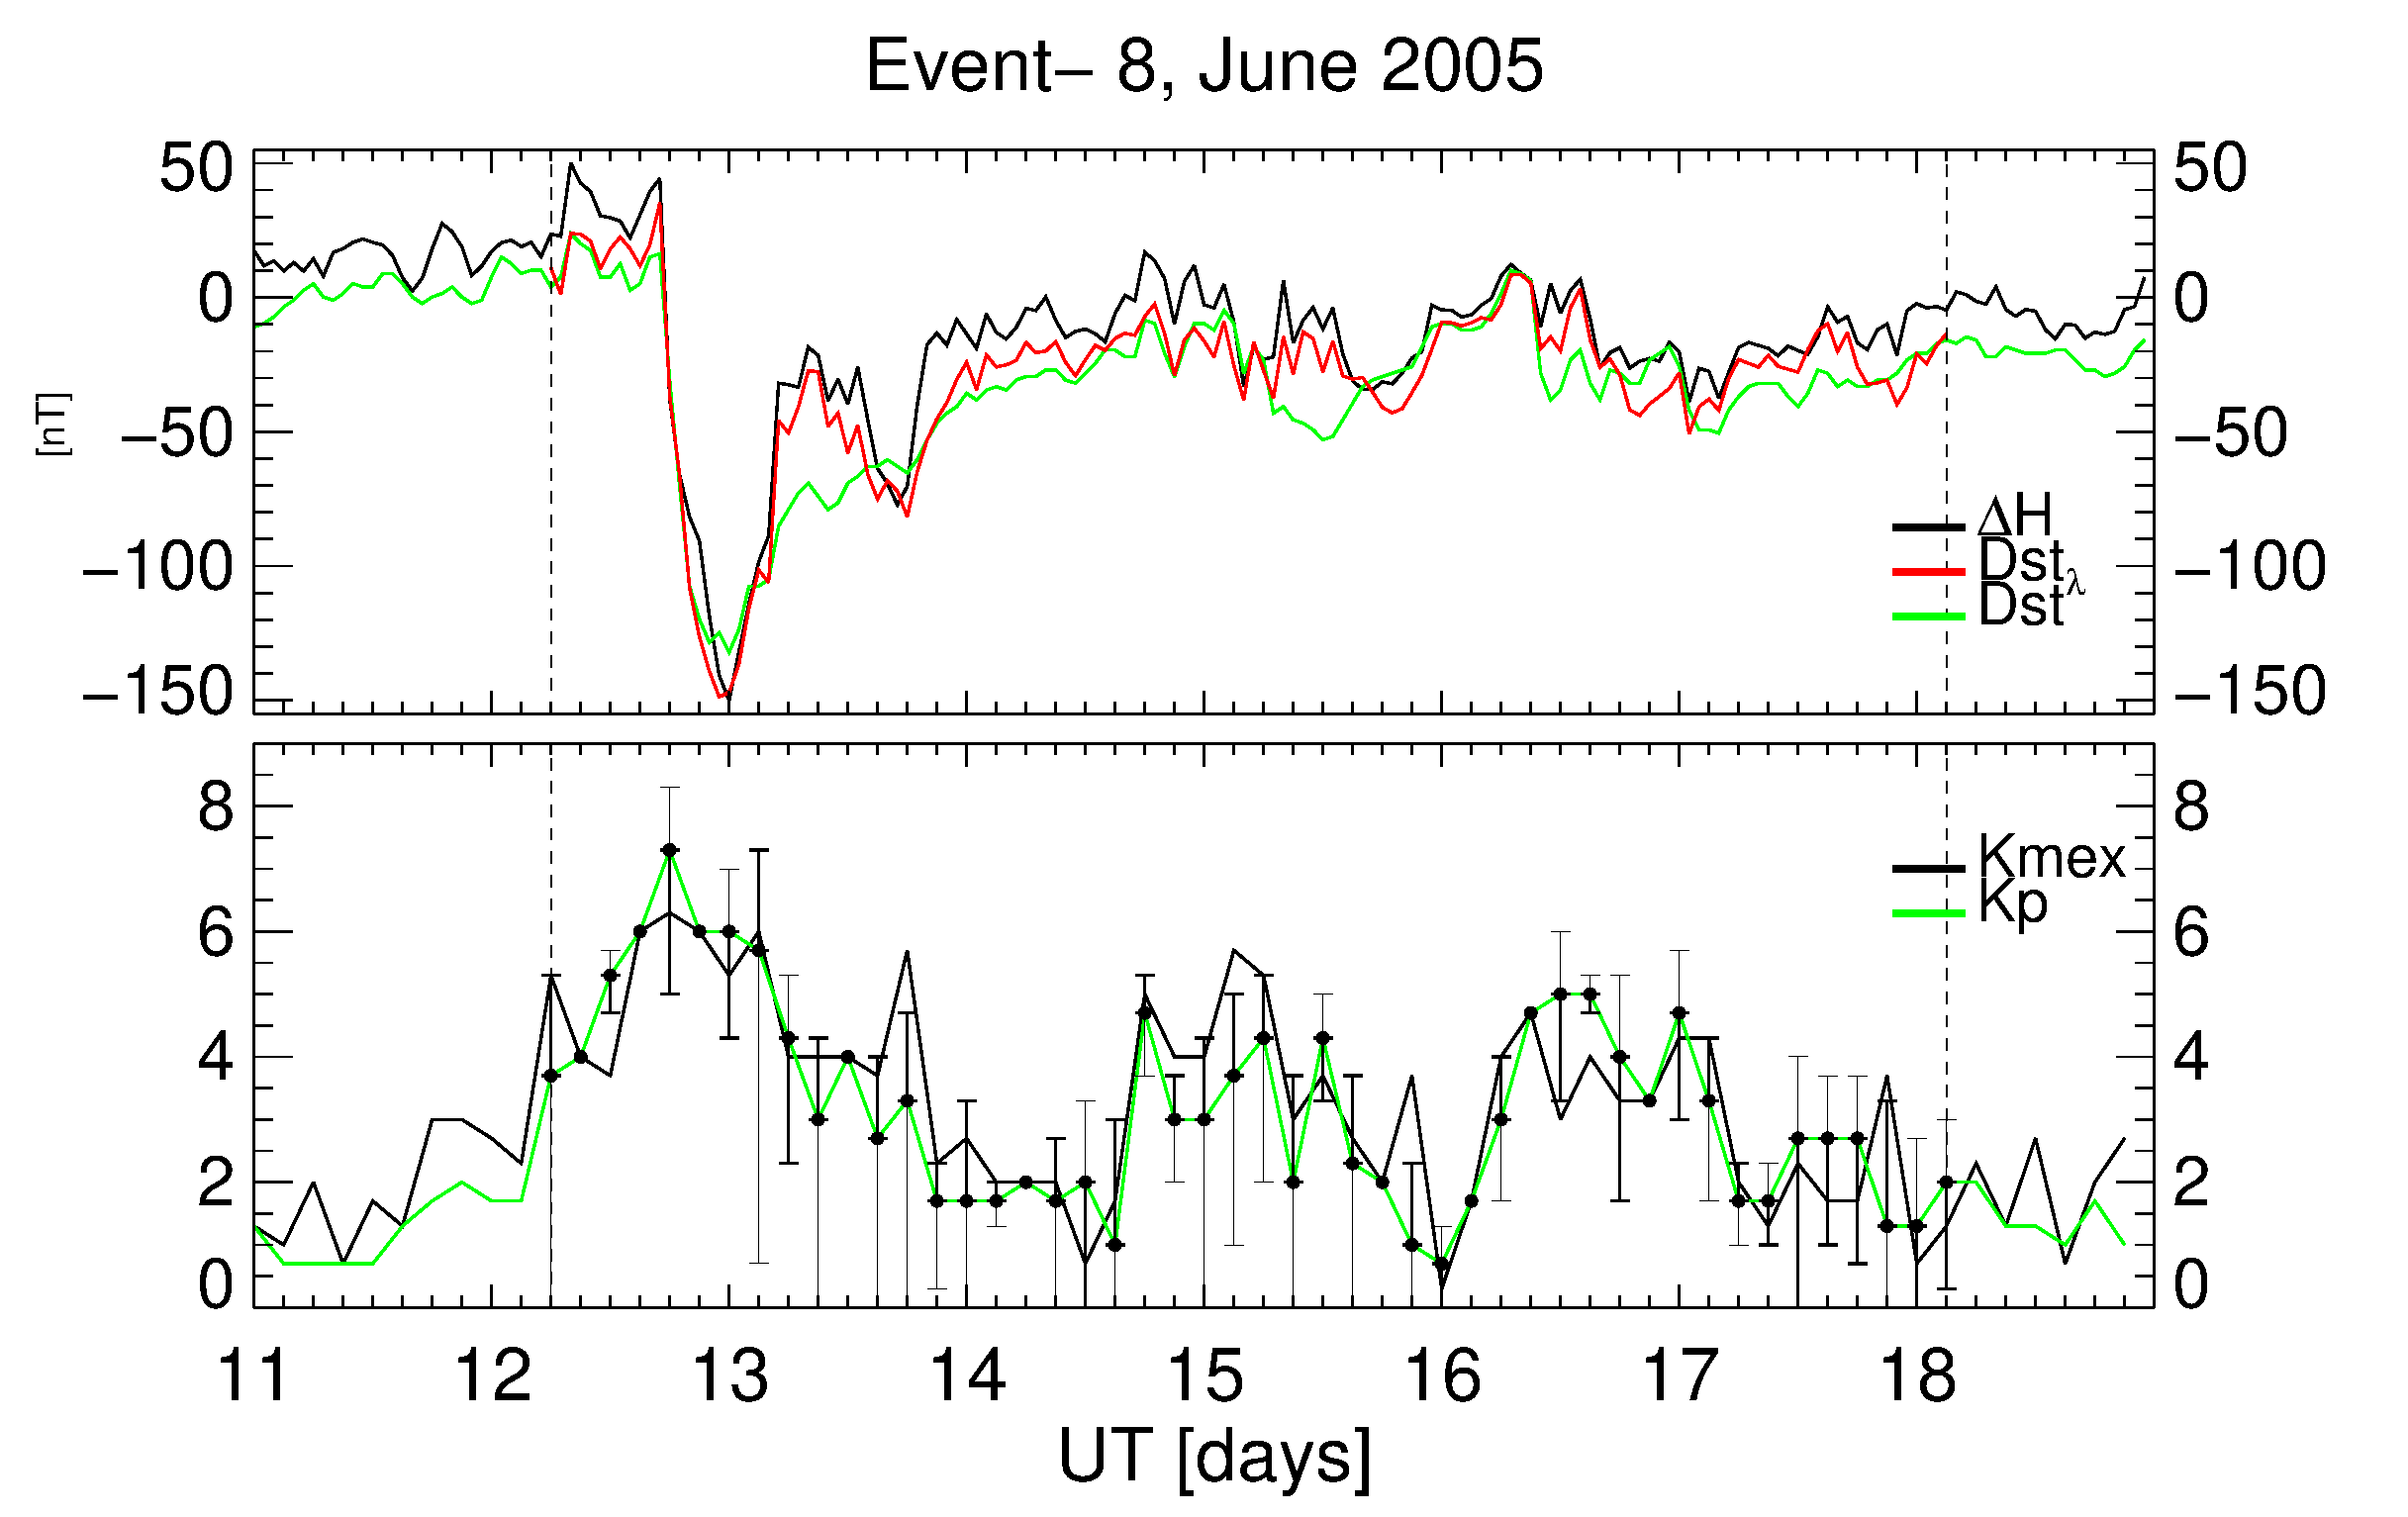
\includegraphics[width=6.0cm]{images/dH_approx/diono_valid_V4_2005-06-11.eps}

       \centerline{\Large \bf   
      \hspace{0.275\textwidth}  \color{black}{}
       \hspace{0.295\textwidth}  \color{black}{}
         \hfill}
       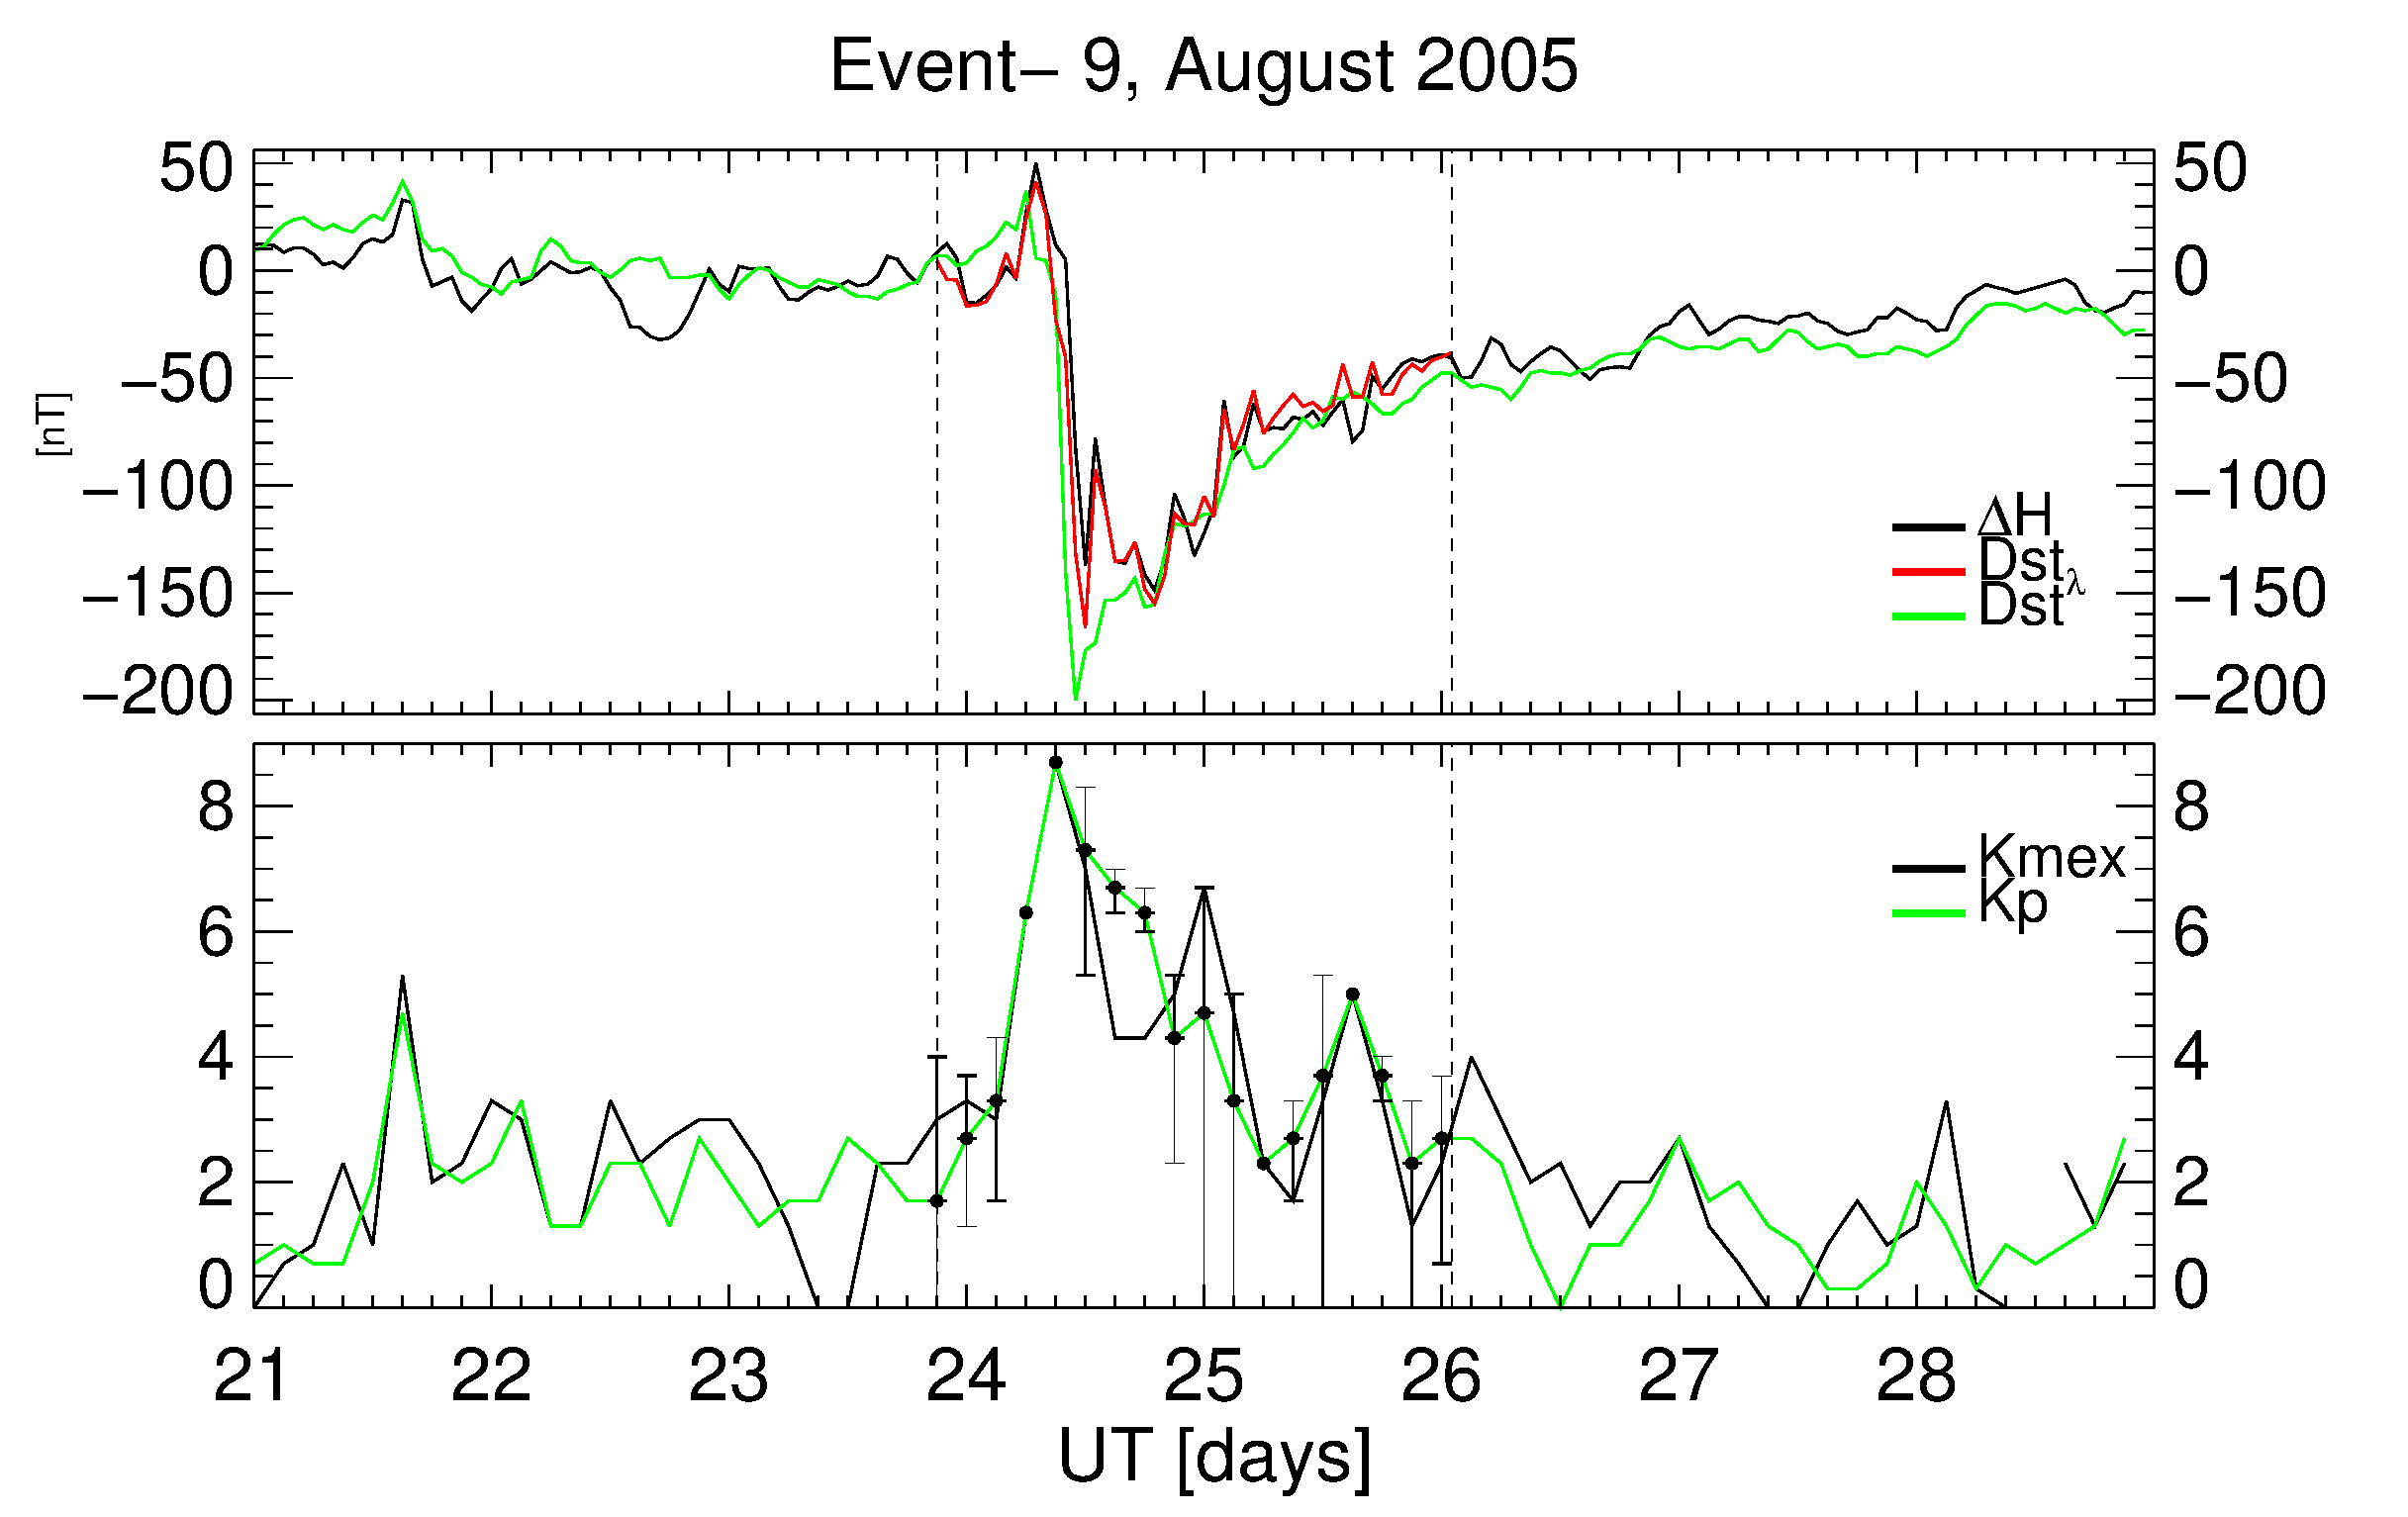
\includegraphics[width=6.0cm]{images/dH_approx/diono_valid_V4_2005-08-21.eps}     
       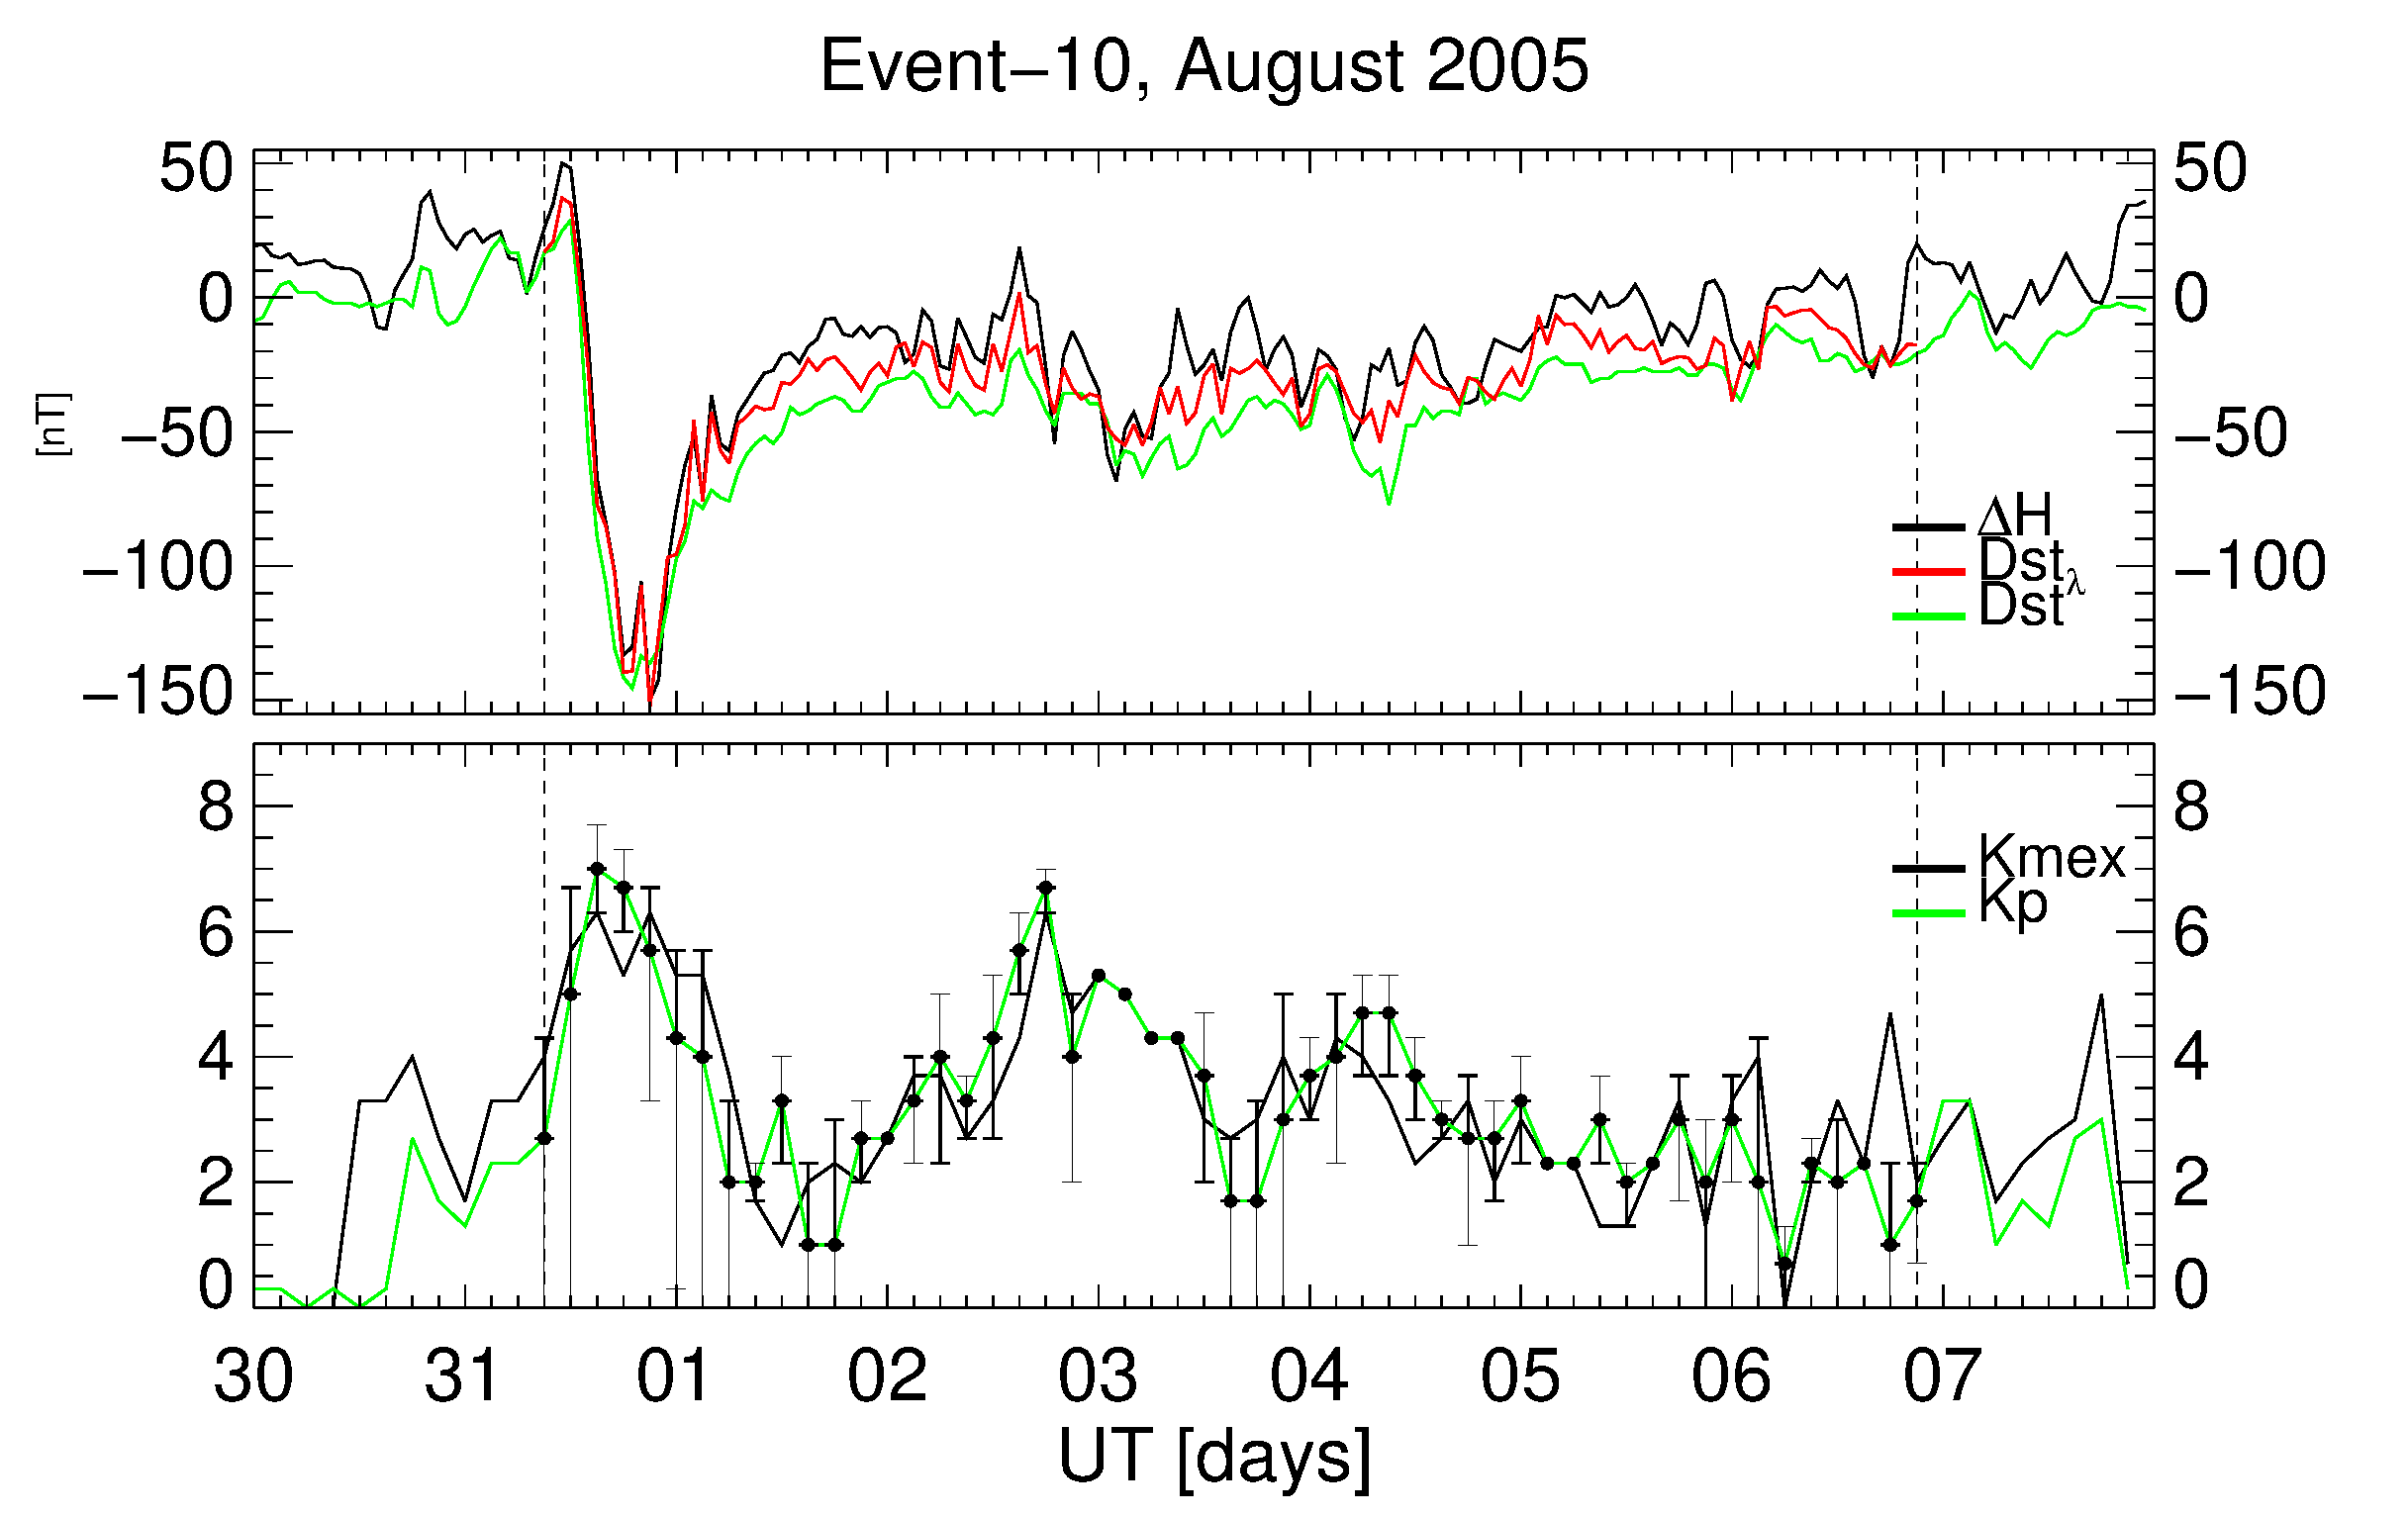
\includegraphics[width=6.0cm]{images/dH_approx/diono_valid_V4_2005-08-30.eps}
       
       \caption{Top: Approximation of $\Delta$H (red line). Bottom: Approximation of K local with a $\Delta$K affection range (error bars). }
    \label{fig:iono_valid2}
\end{figure*}


\begin{figure*}[h!]
    \centering
    \centerline{\Large \bf   
      %\hspace{0.18\textwidth}  \color{black}{\Large{Res}}
       %\hspace{0.28\textwidth}  \color{black}{\Large{Res+TC}}
         \hfill}
          \centerline{\Large \bf   
      \hspace{0.26\textwidth}  \color{black}{}
       \hspace{0.31\textwidth}  \color{black}{}
         \hfill}
     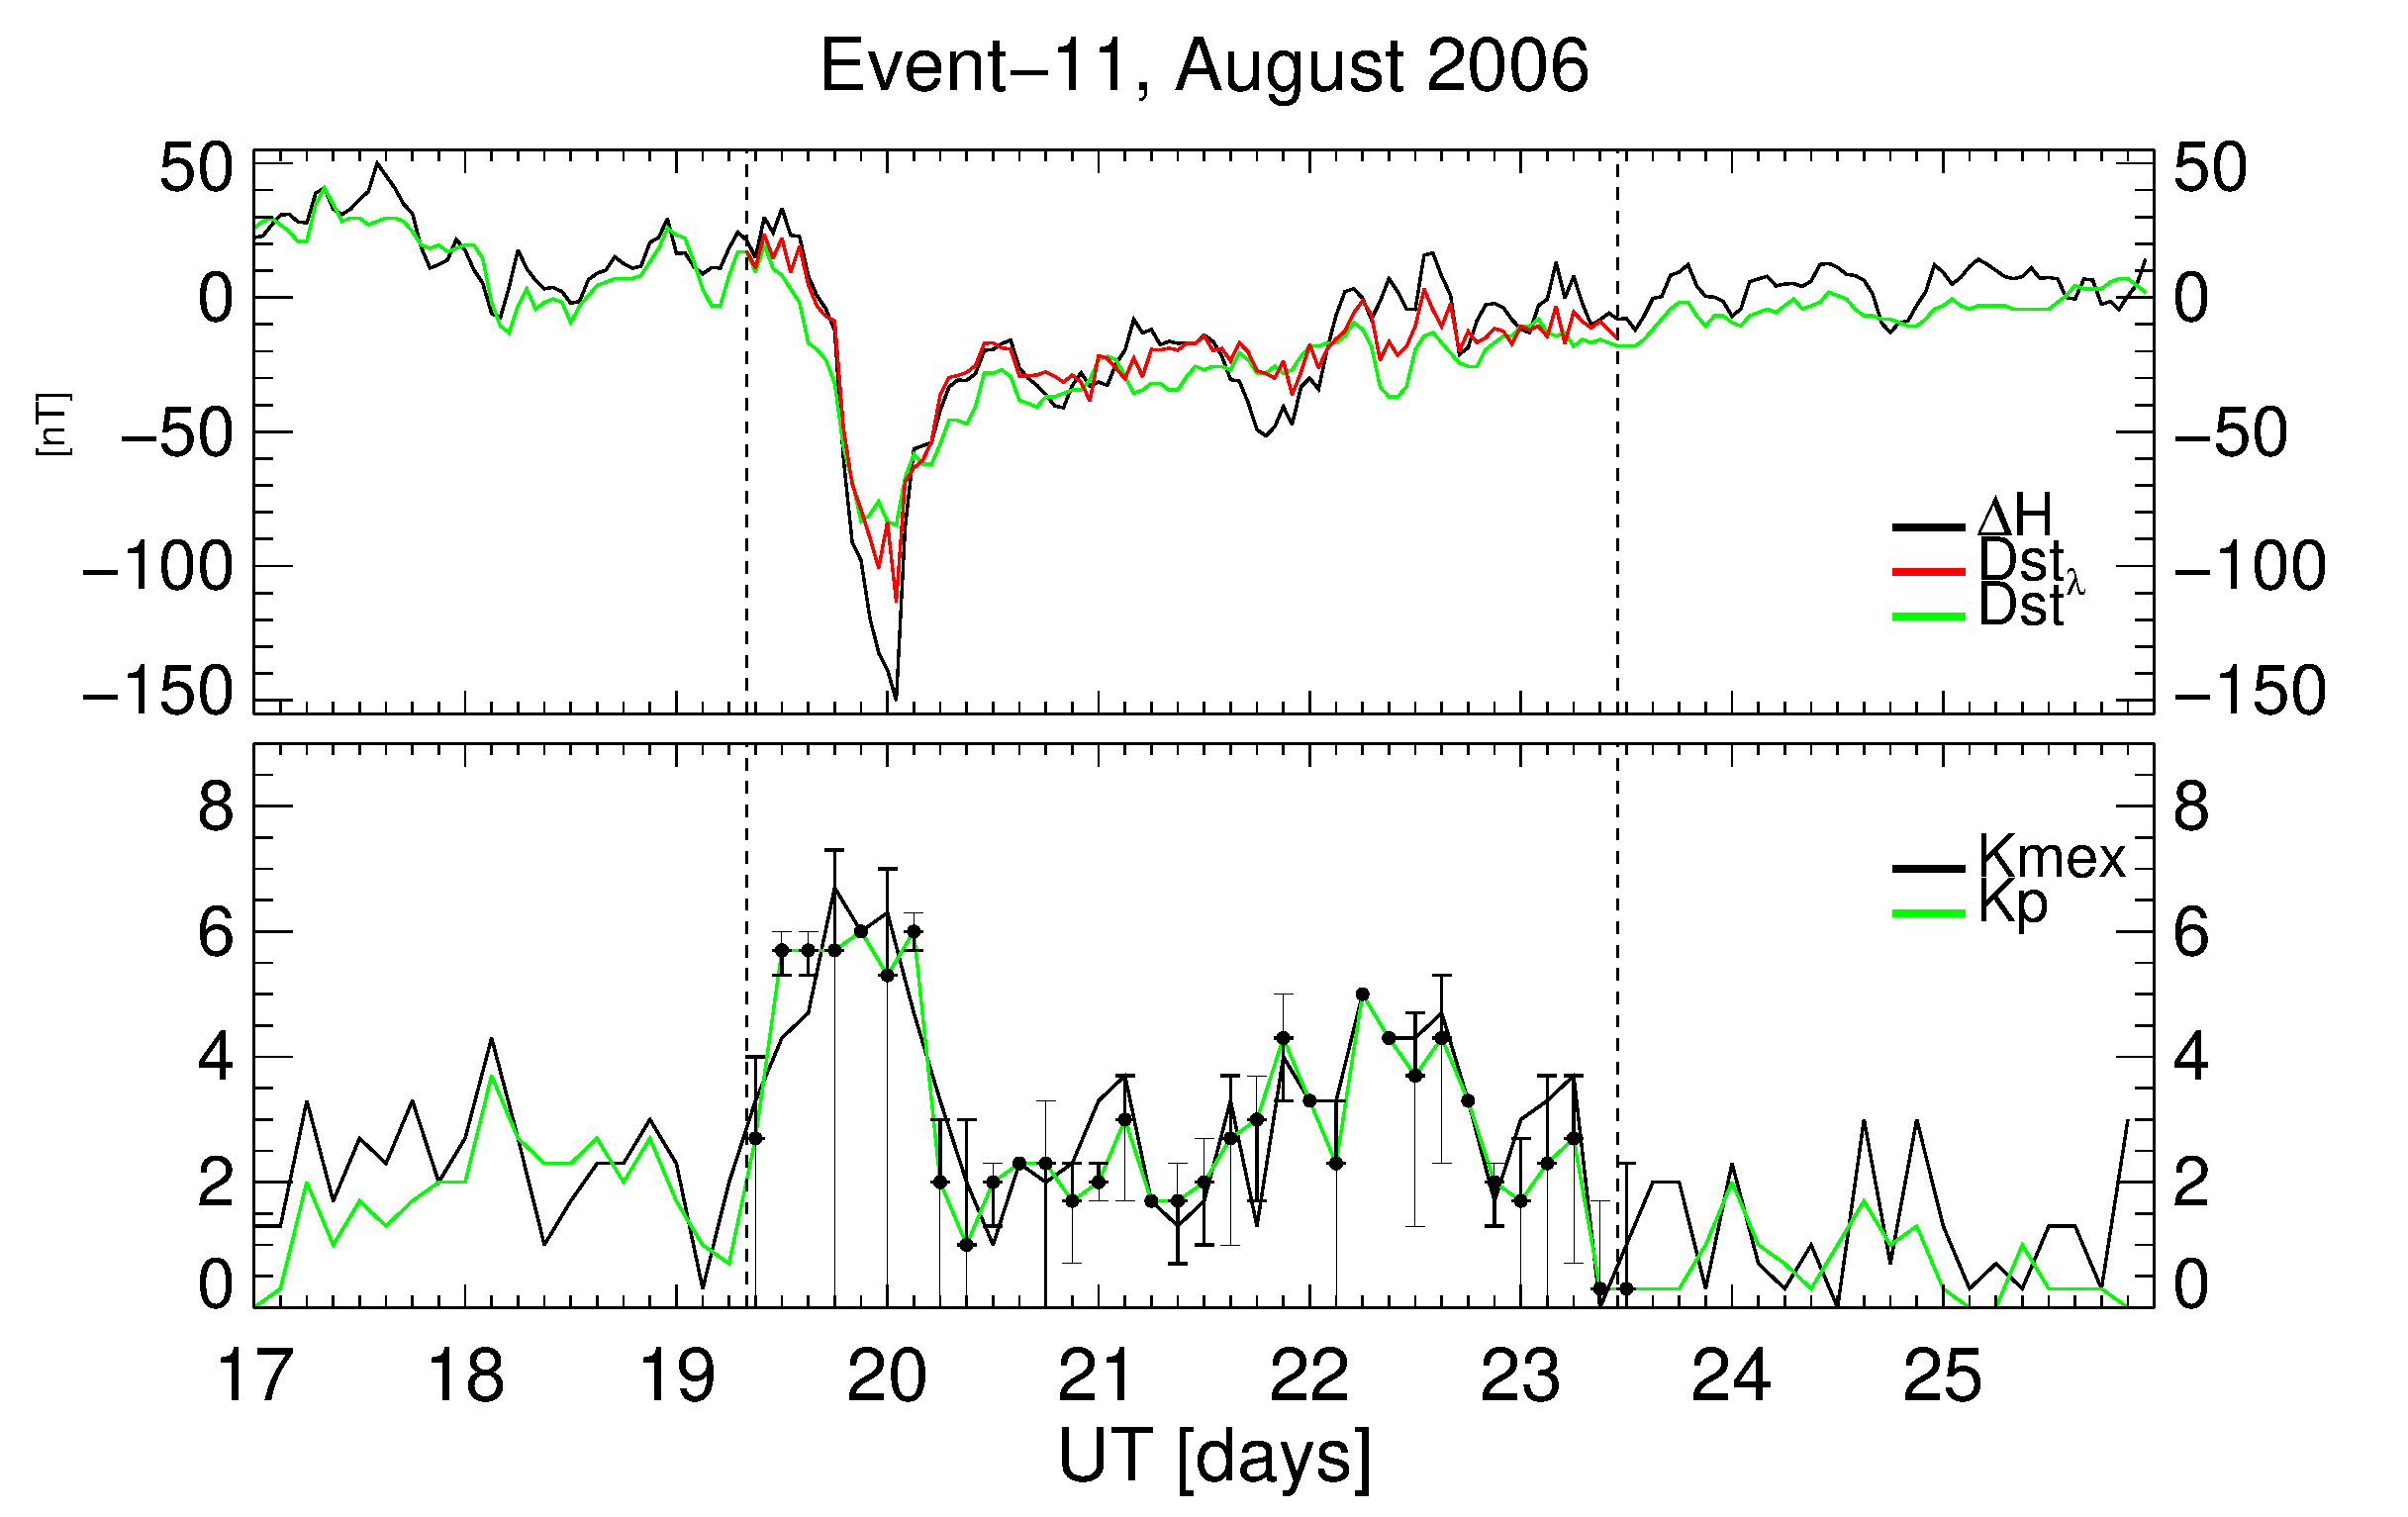
\includegraphics[width=6.0cm]{images/dH_approx/diono_valid_V4_2006-08-17.eps}
     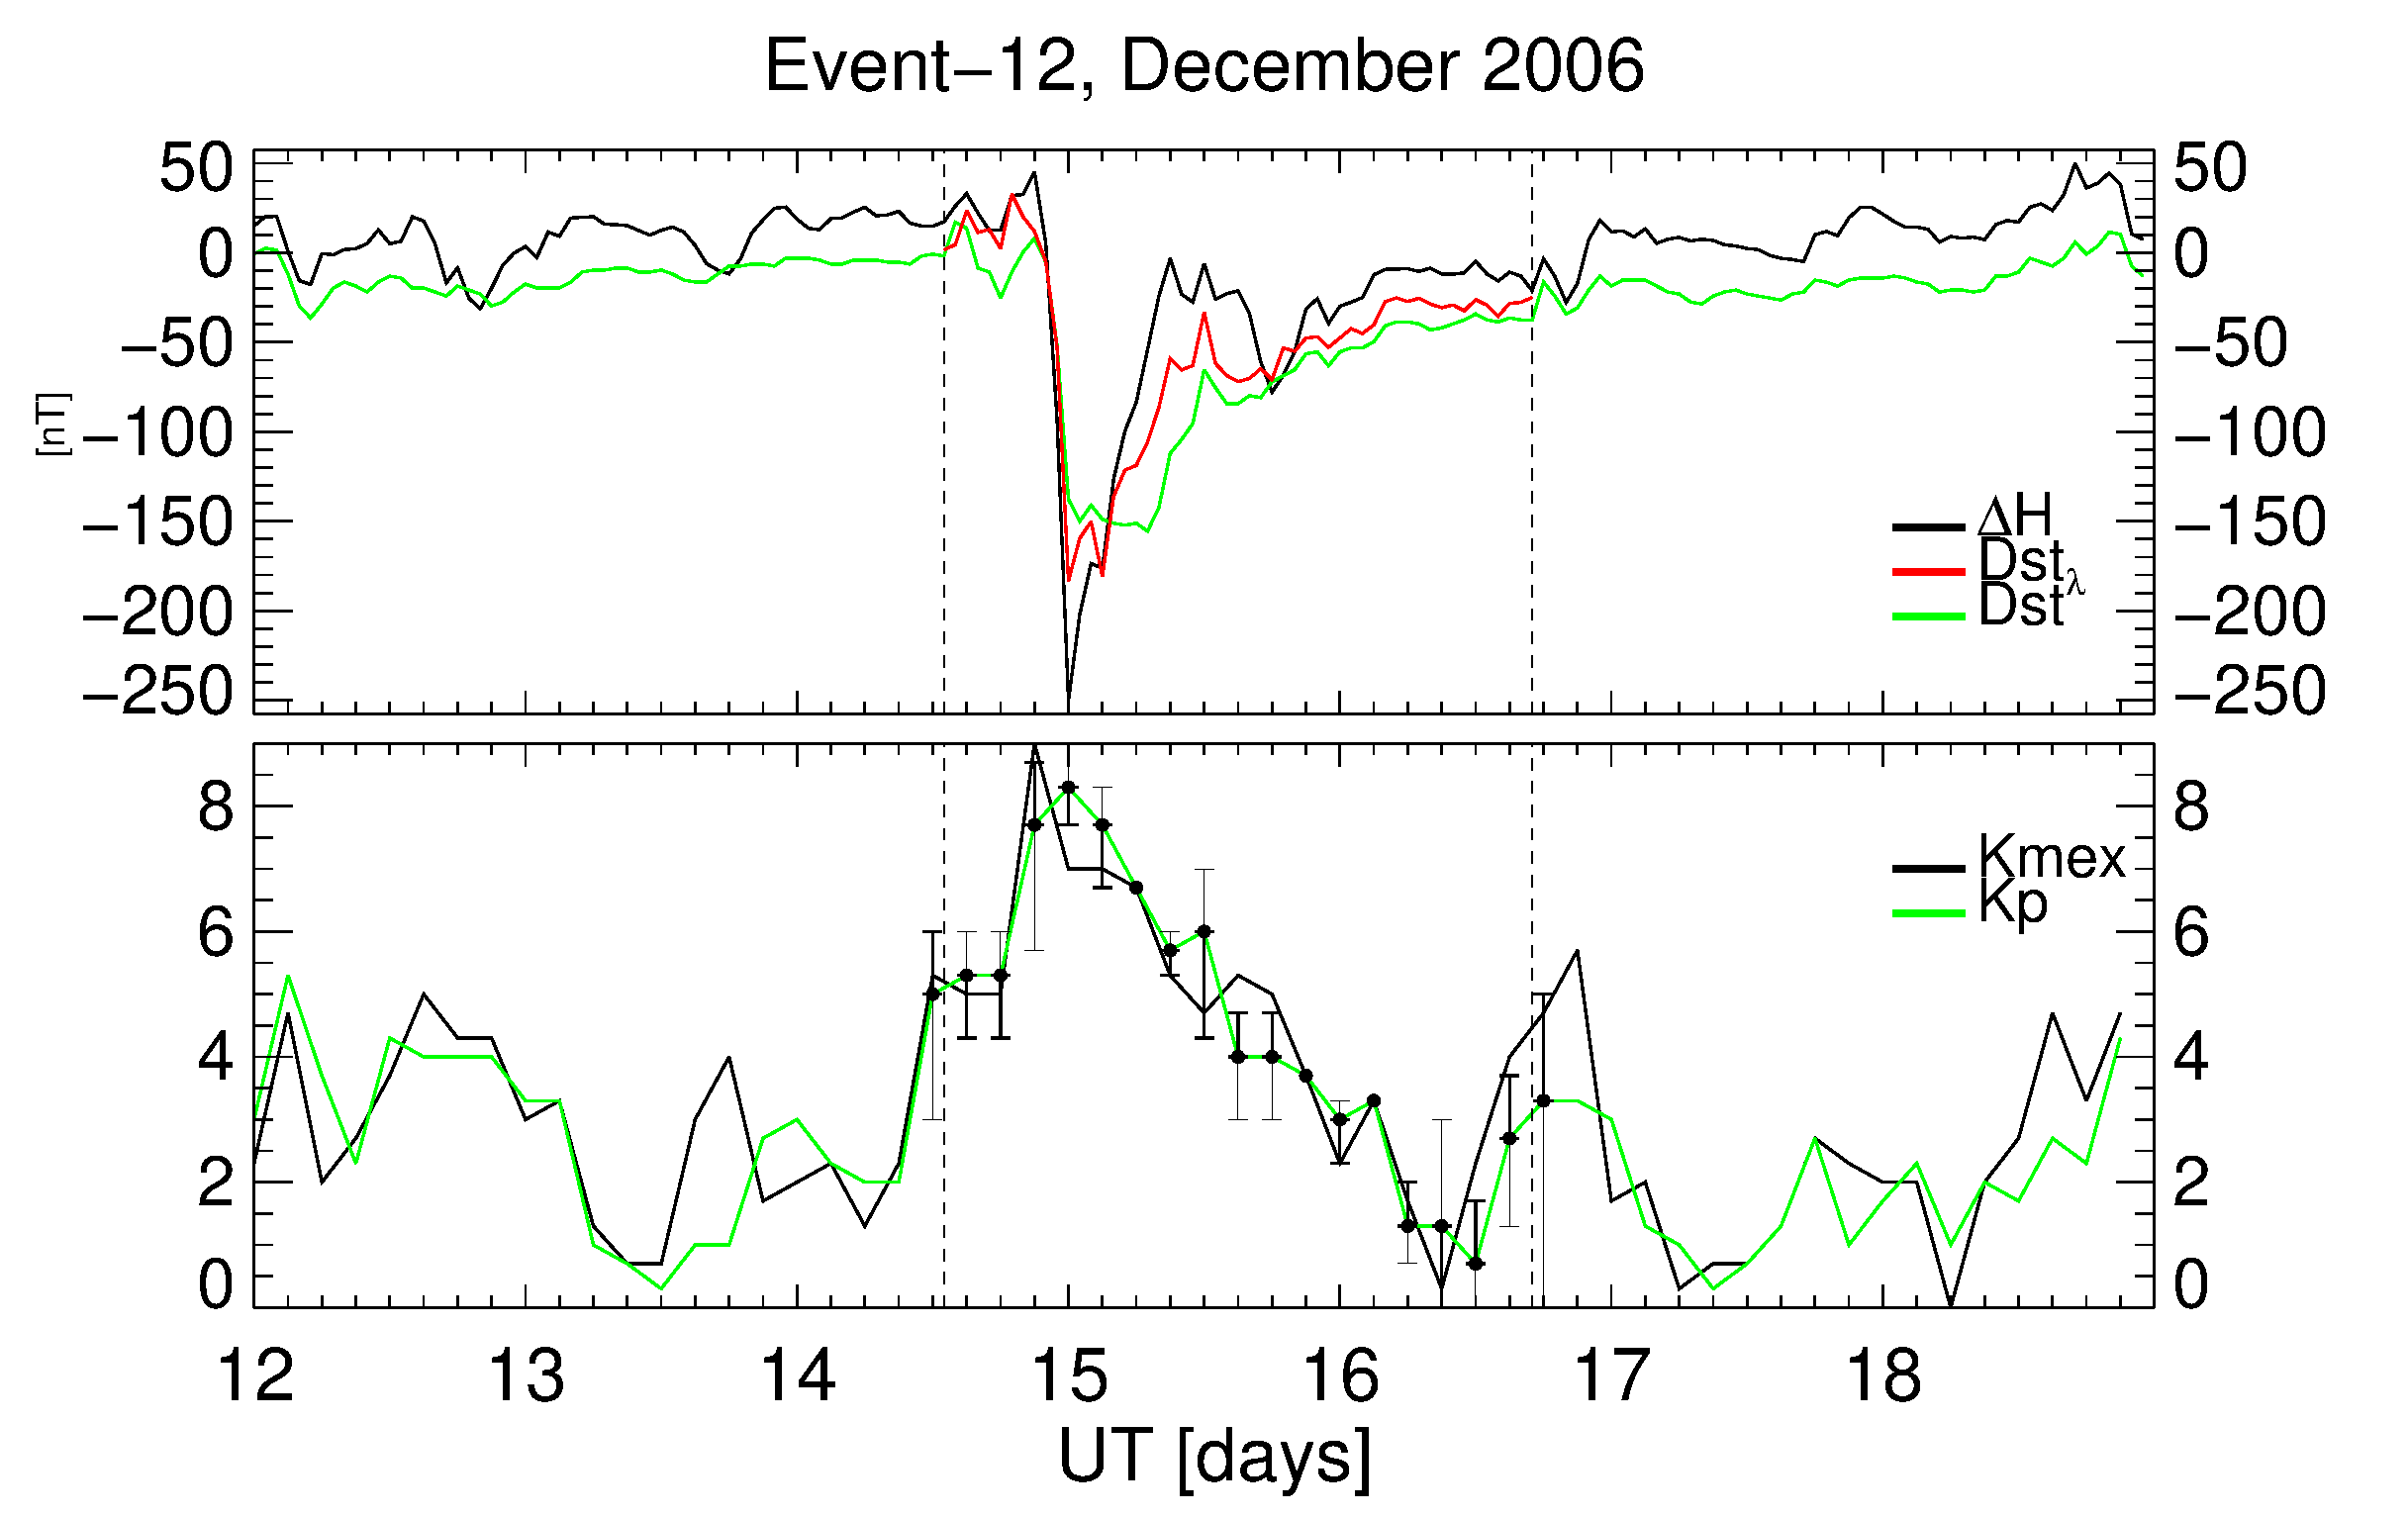
\includegraphics[width=6.0cm]{images/dH_approx/diono_valid_V4_2006-12-12.eps}
     \centerline{\Large \bf   
      \hspace{0.275\textwidth}  \color{black}{}
       \hspace{0.295\textwidth}  \color{black}{}
         \hfill}
     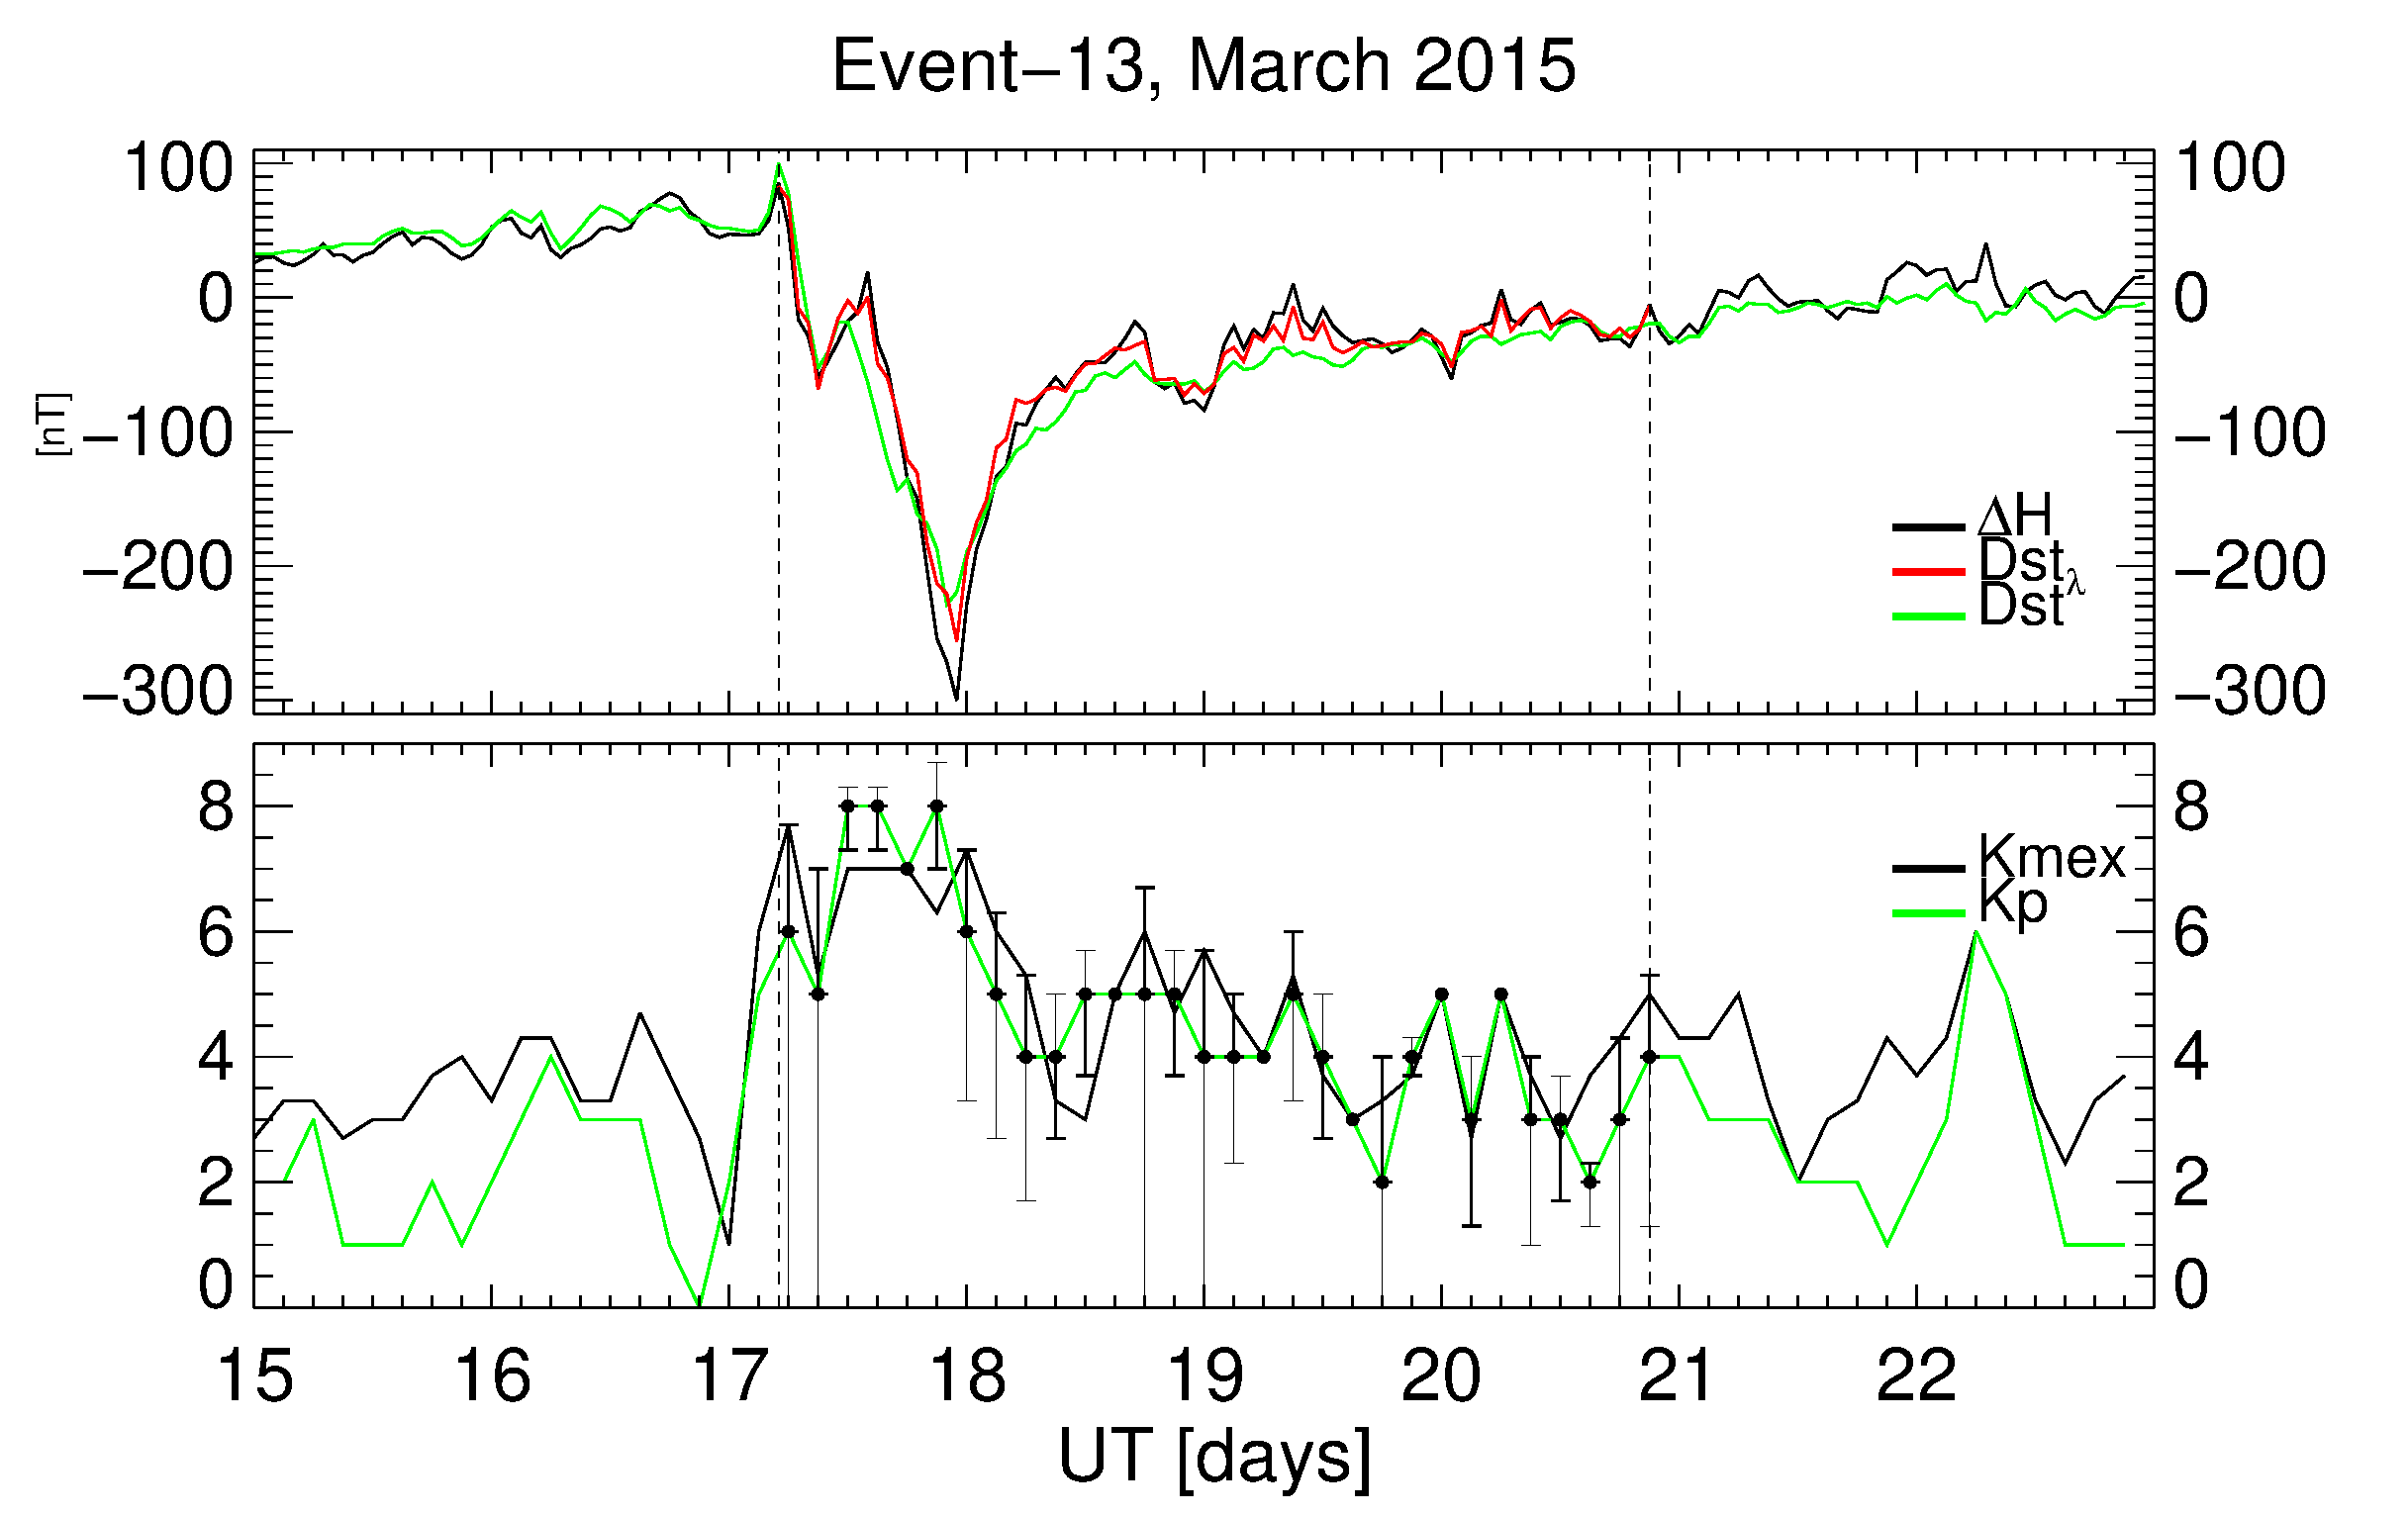
\includegraphics[width=6.0cm]{images/dH_approx/diono_valid_V4_2015-03-15.eps}     
     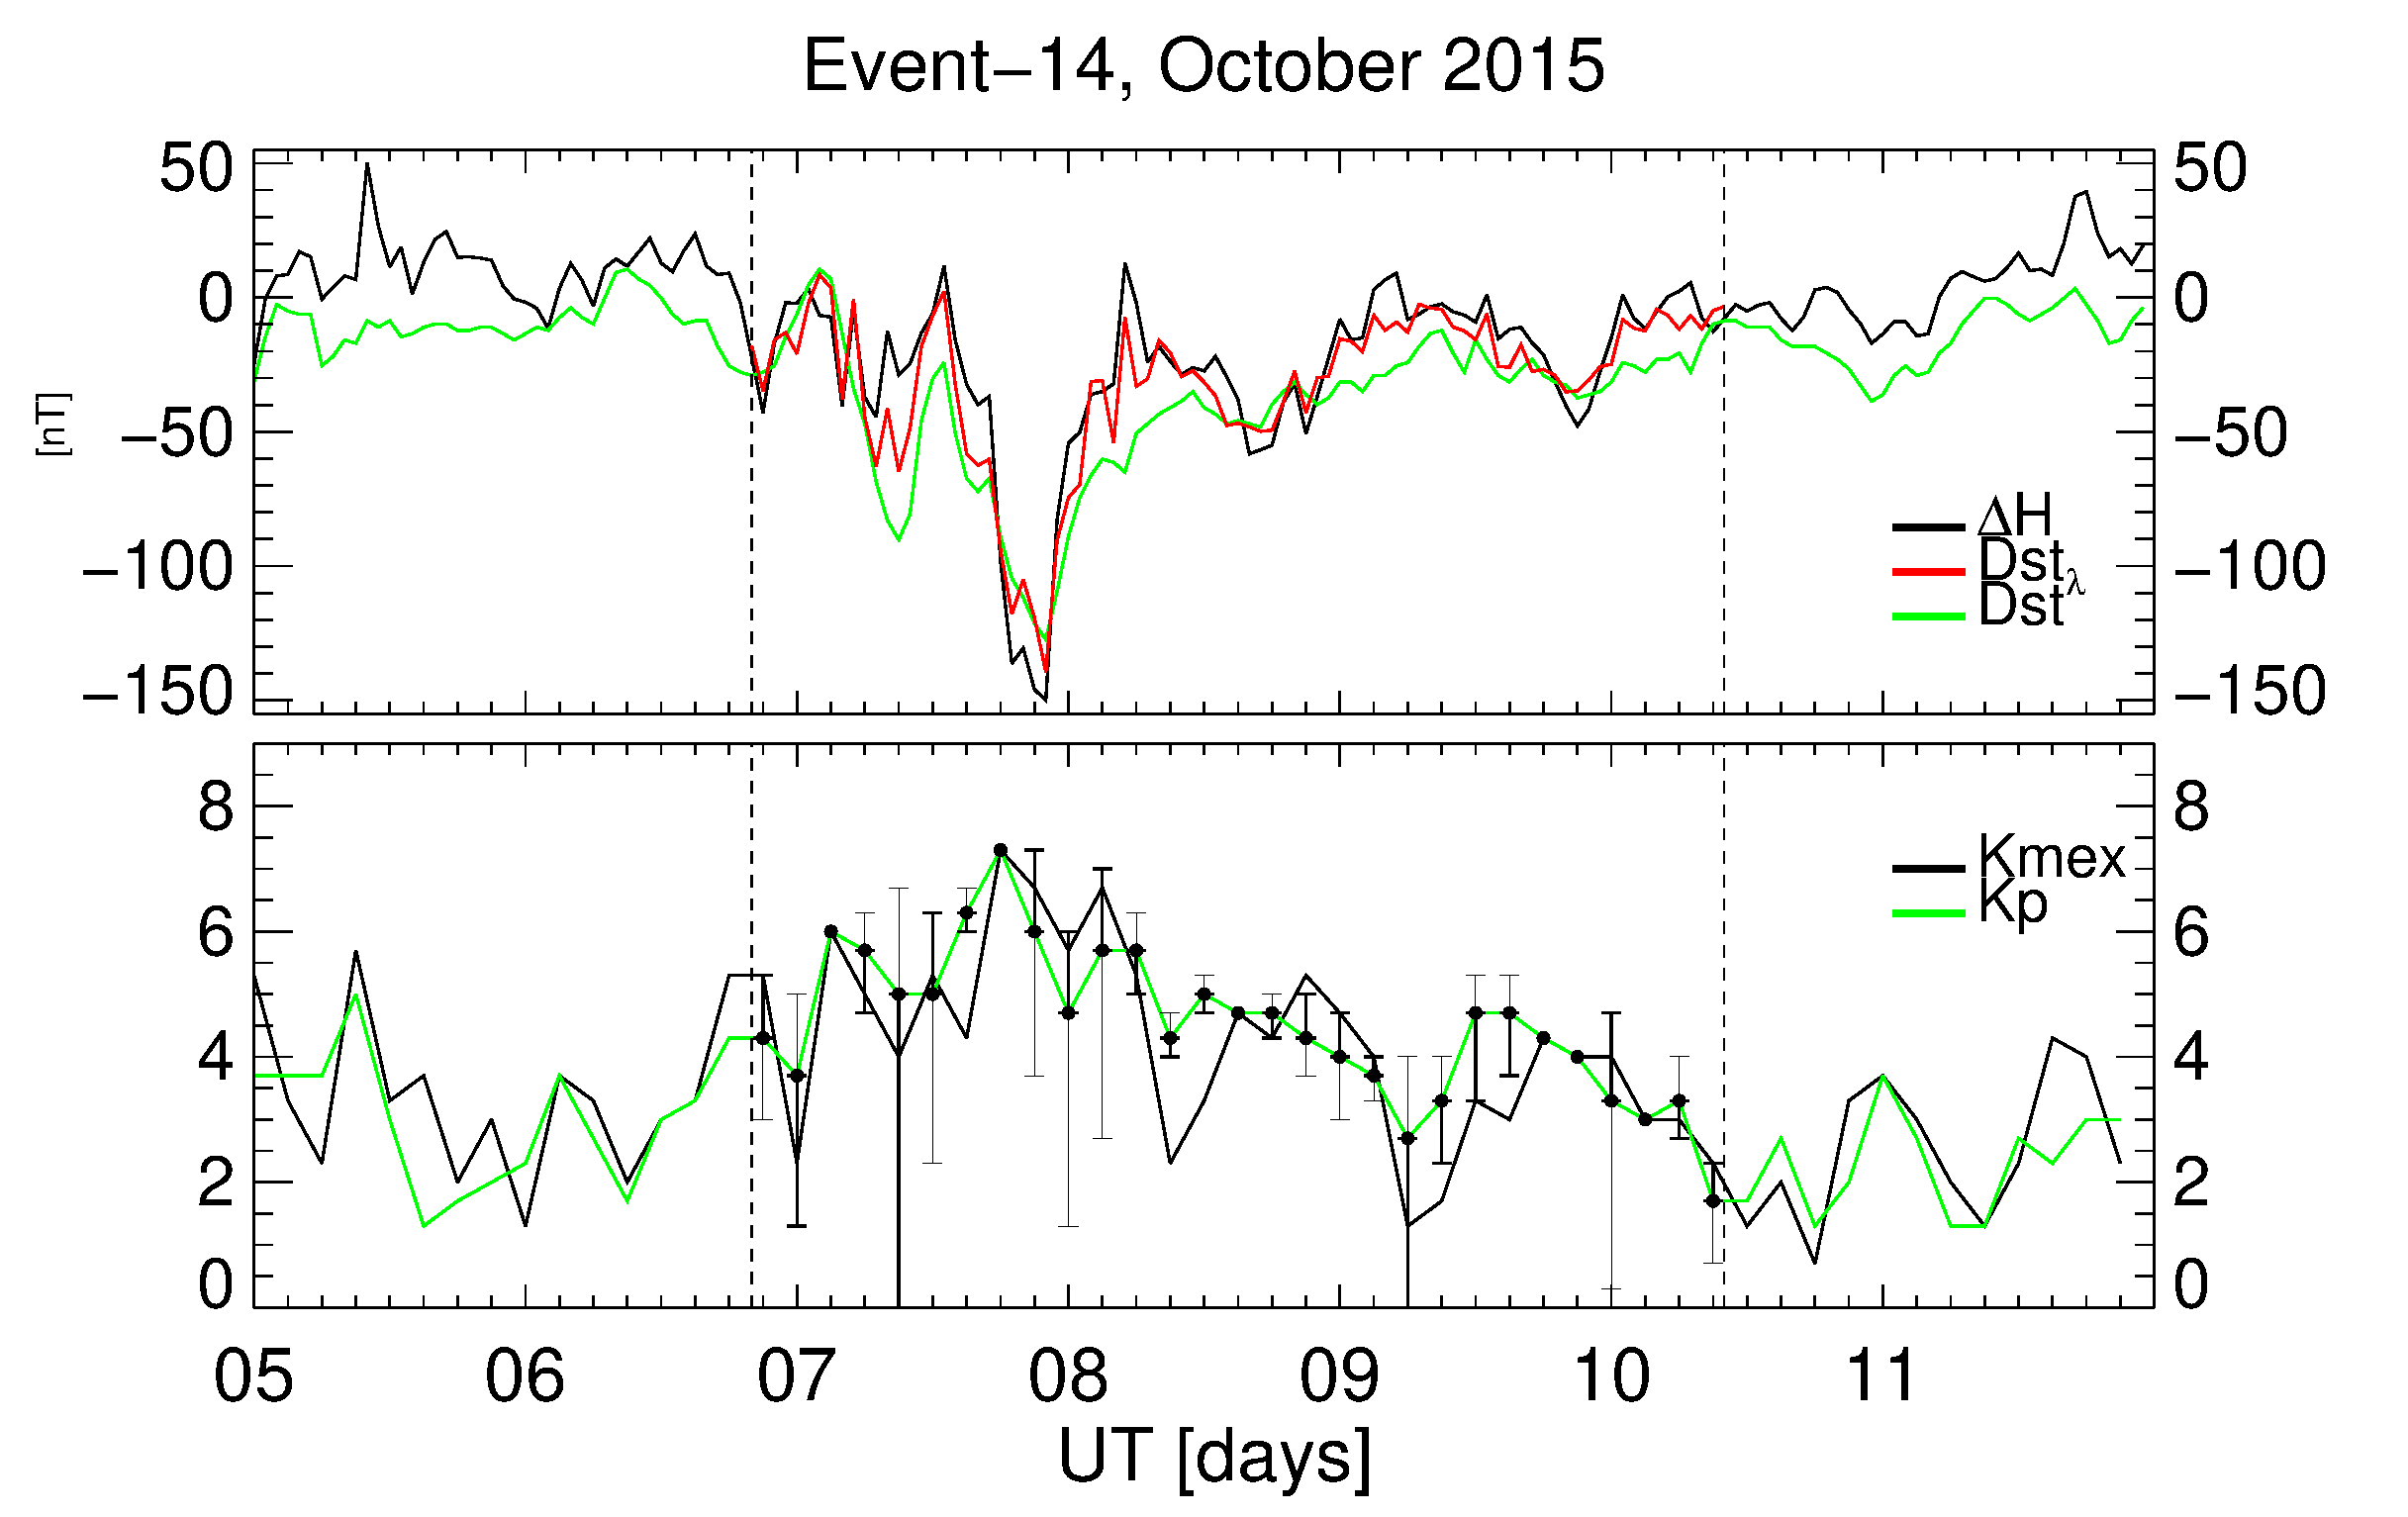
\includegraphics[width=6.0cm]{images/dH_approx/diono_valid_V4_2015-10-05.eps}
     \centerline{\Large \bf   
      \hspace{0.275\textwidth}  \color{black}{}
       \hspace{0.295\textwidth}  \color{black}{}
         \hfill}
      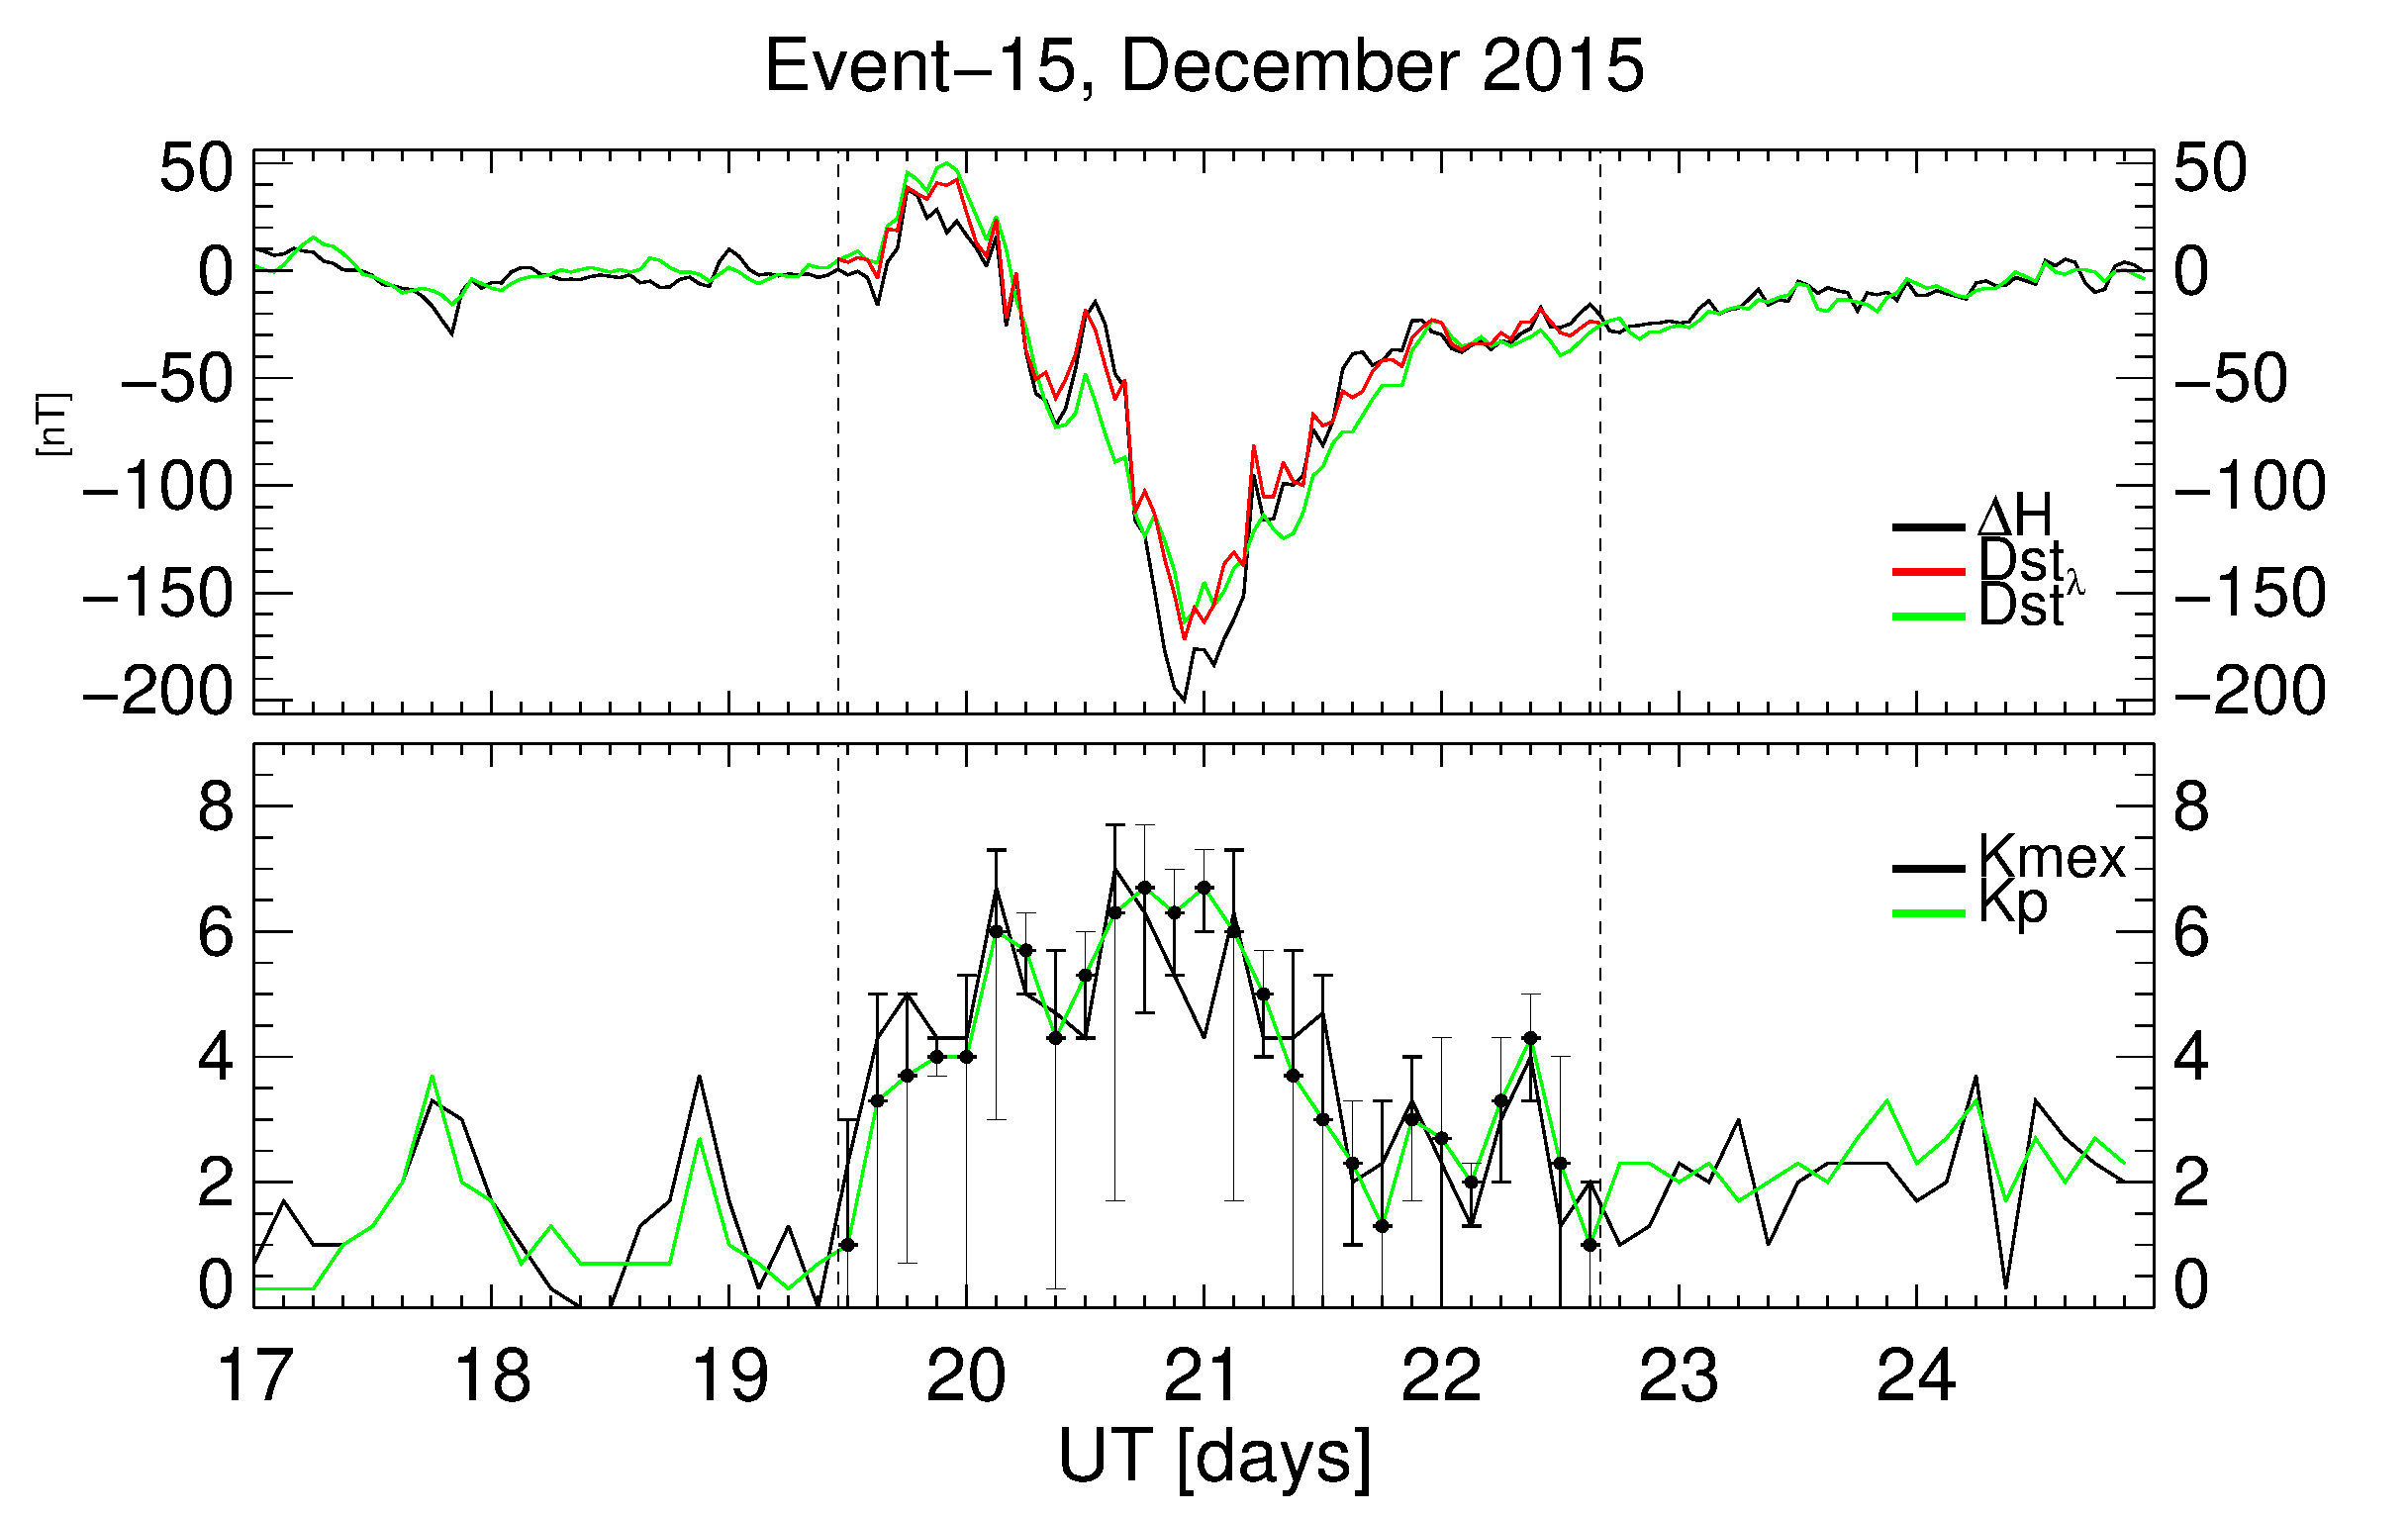
\includegraphics[width=6.0cm]{images/dH_approx/diono_valid_V4_2015-12-17.eps}     
      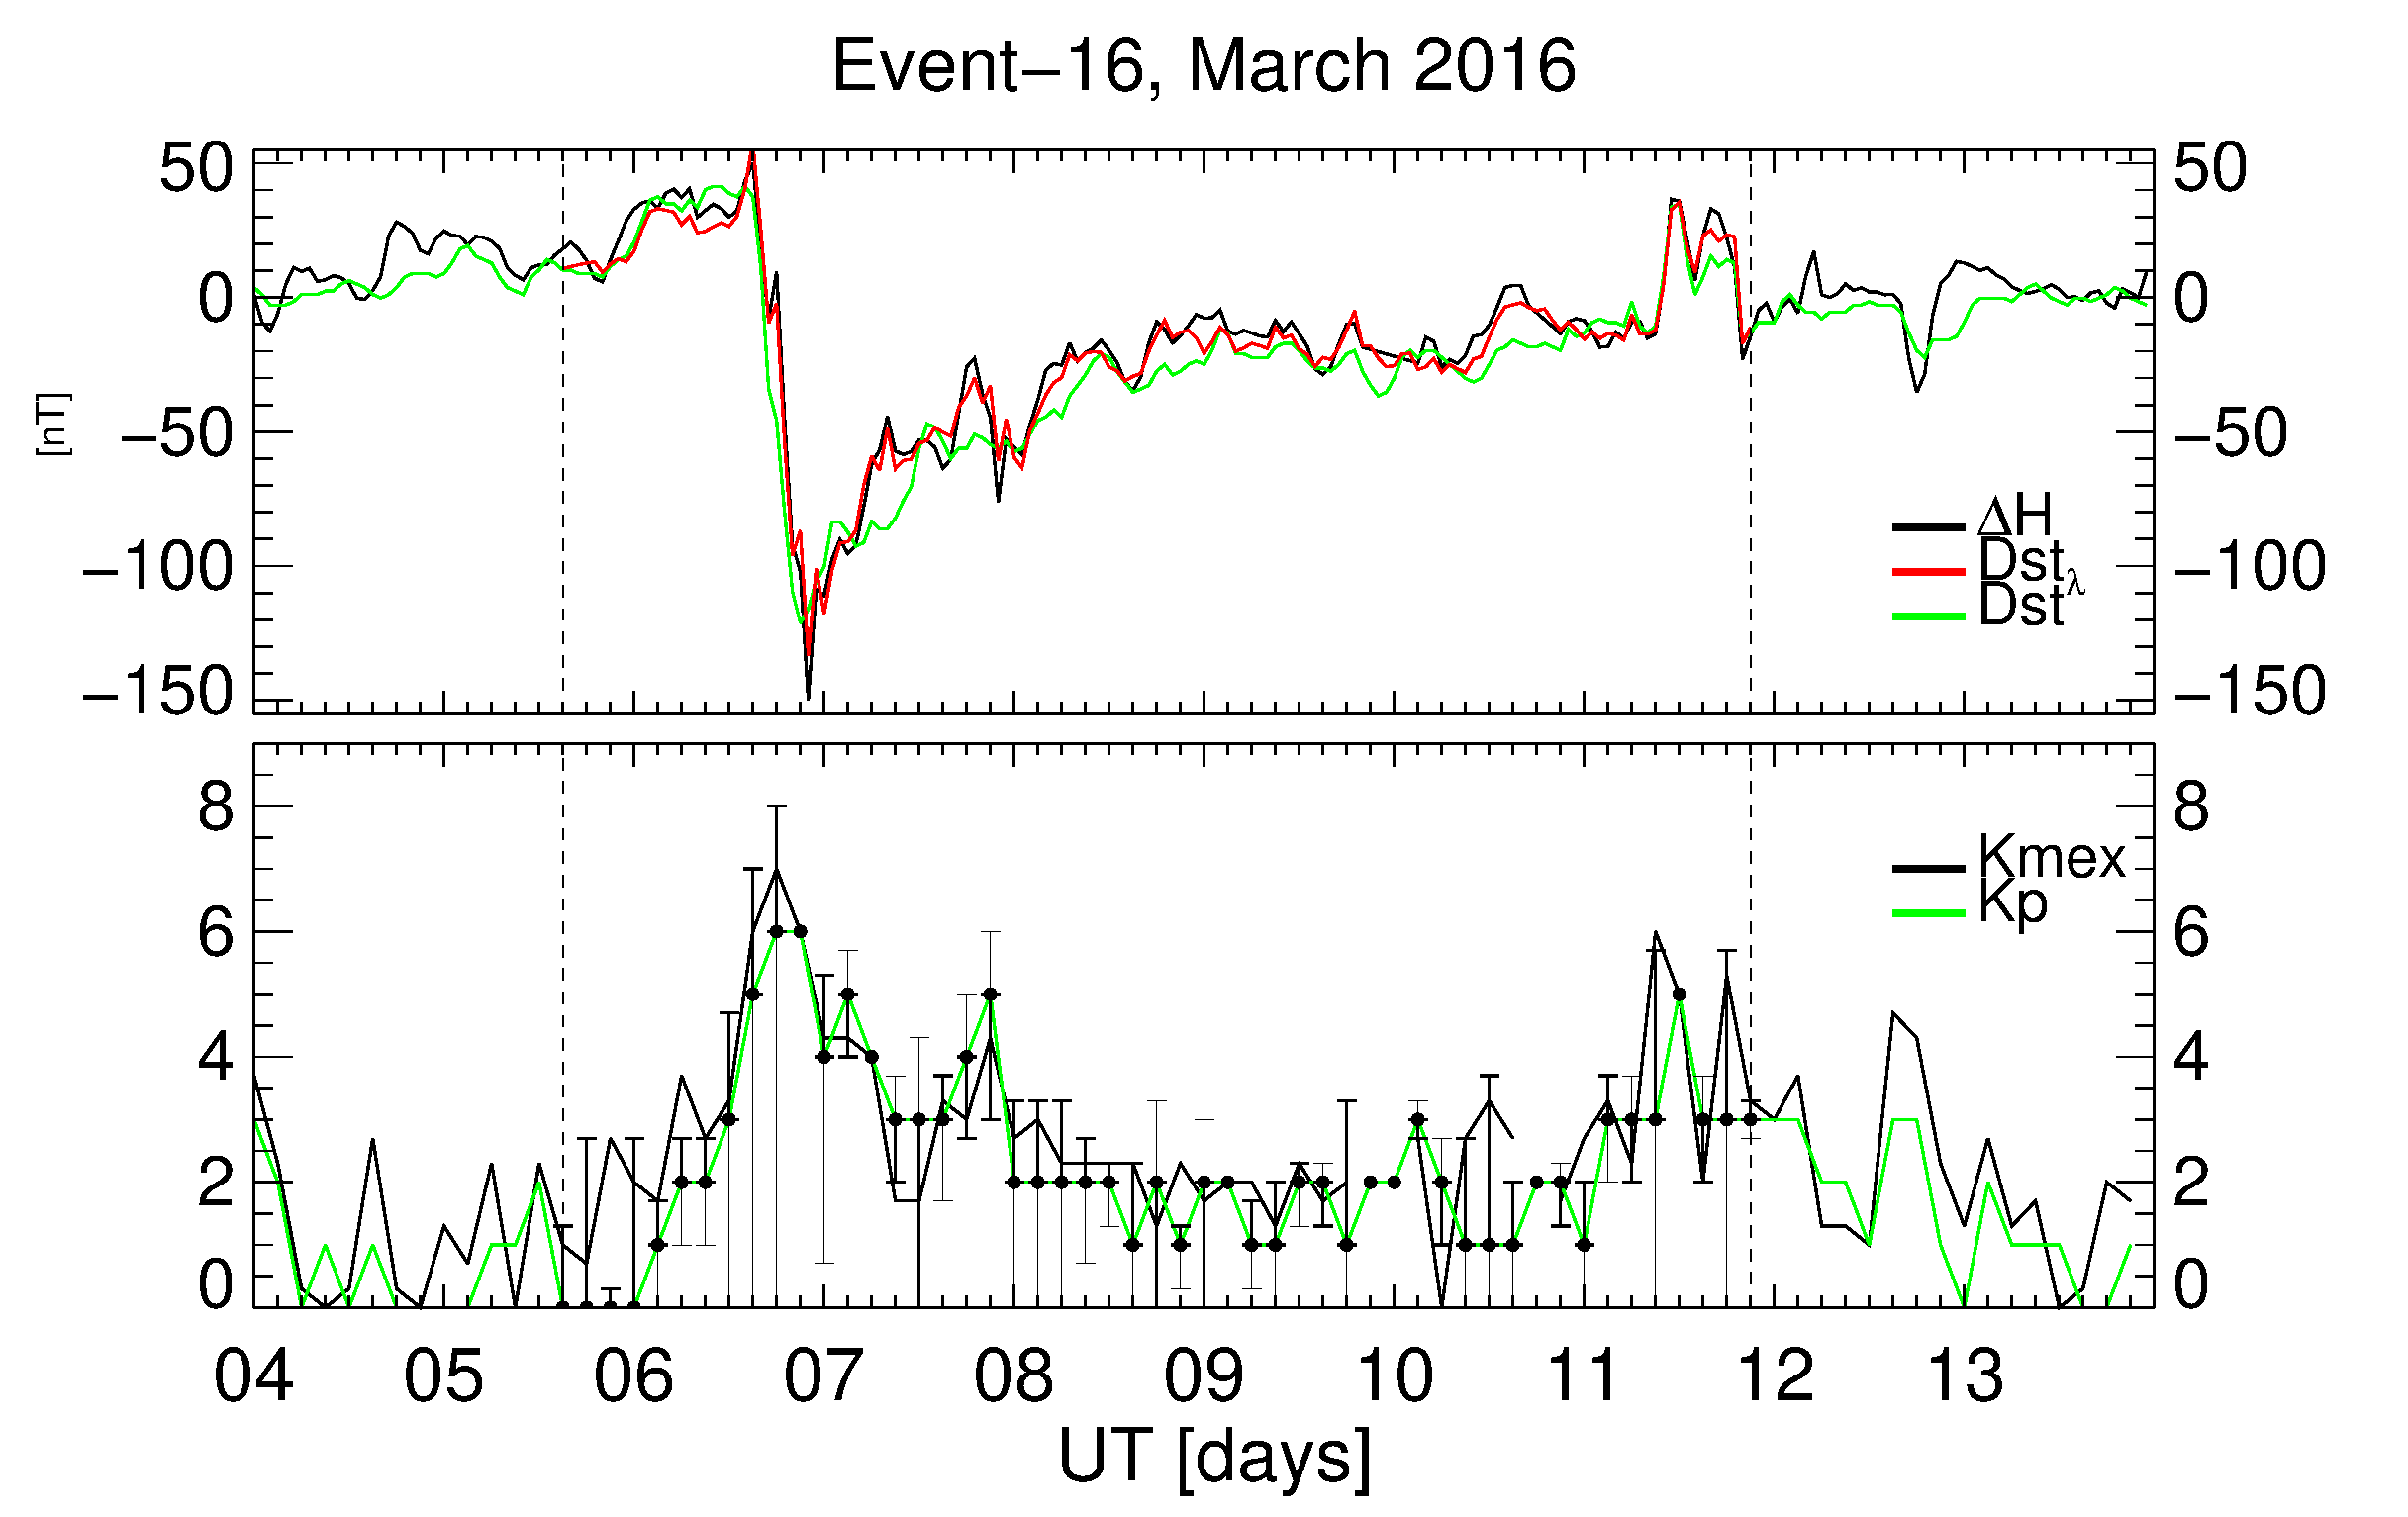
\includegraphics[width=6.0cm]{images/dH_approx/diono_valid_V4_2016-03-04.eps}
       \centerline{\Large \bf   
      \hspace{0.275\textwidth}  \color{black}{}
       \hspace{0.295\textwidth}  \color{black}{}
         \hfill}
       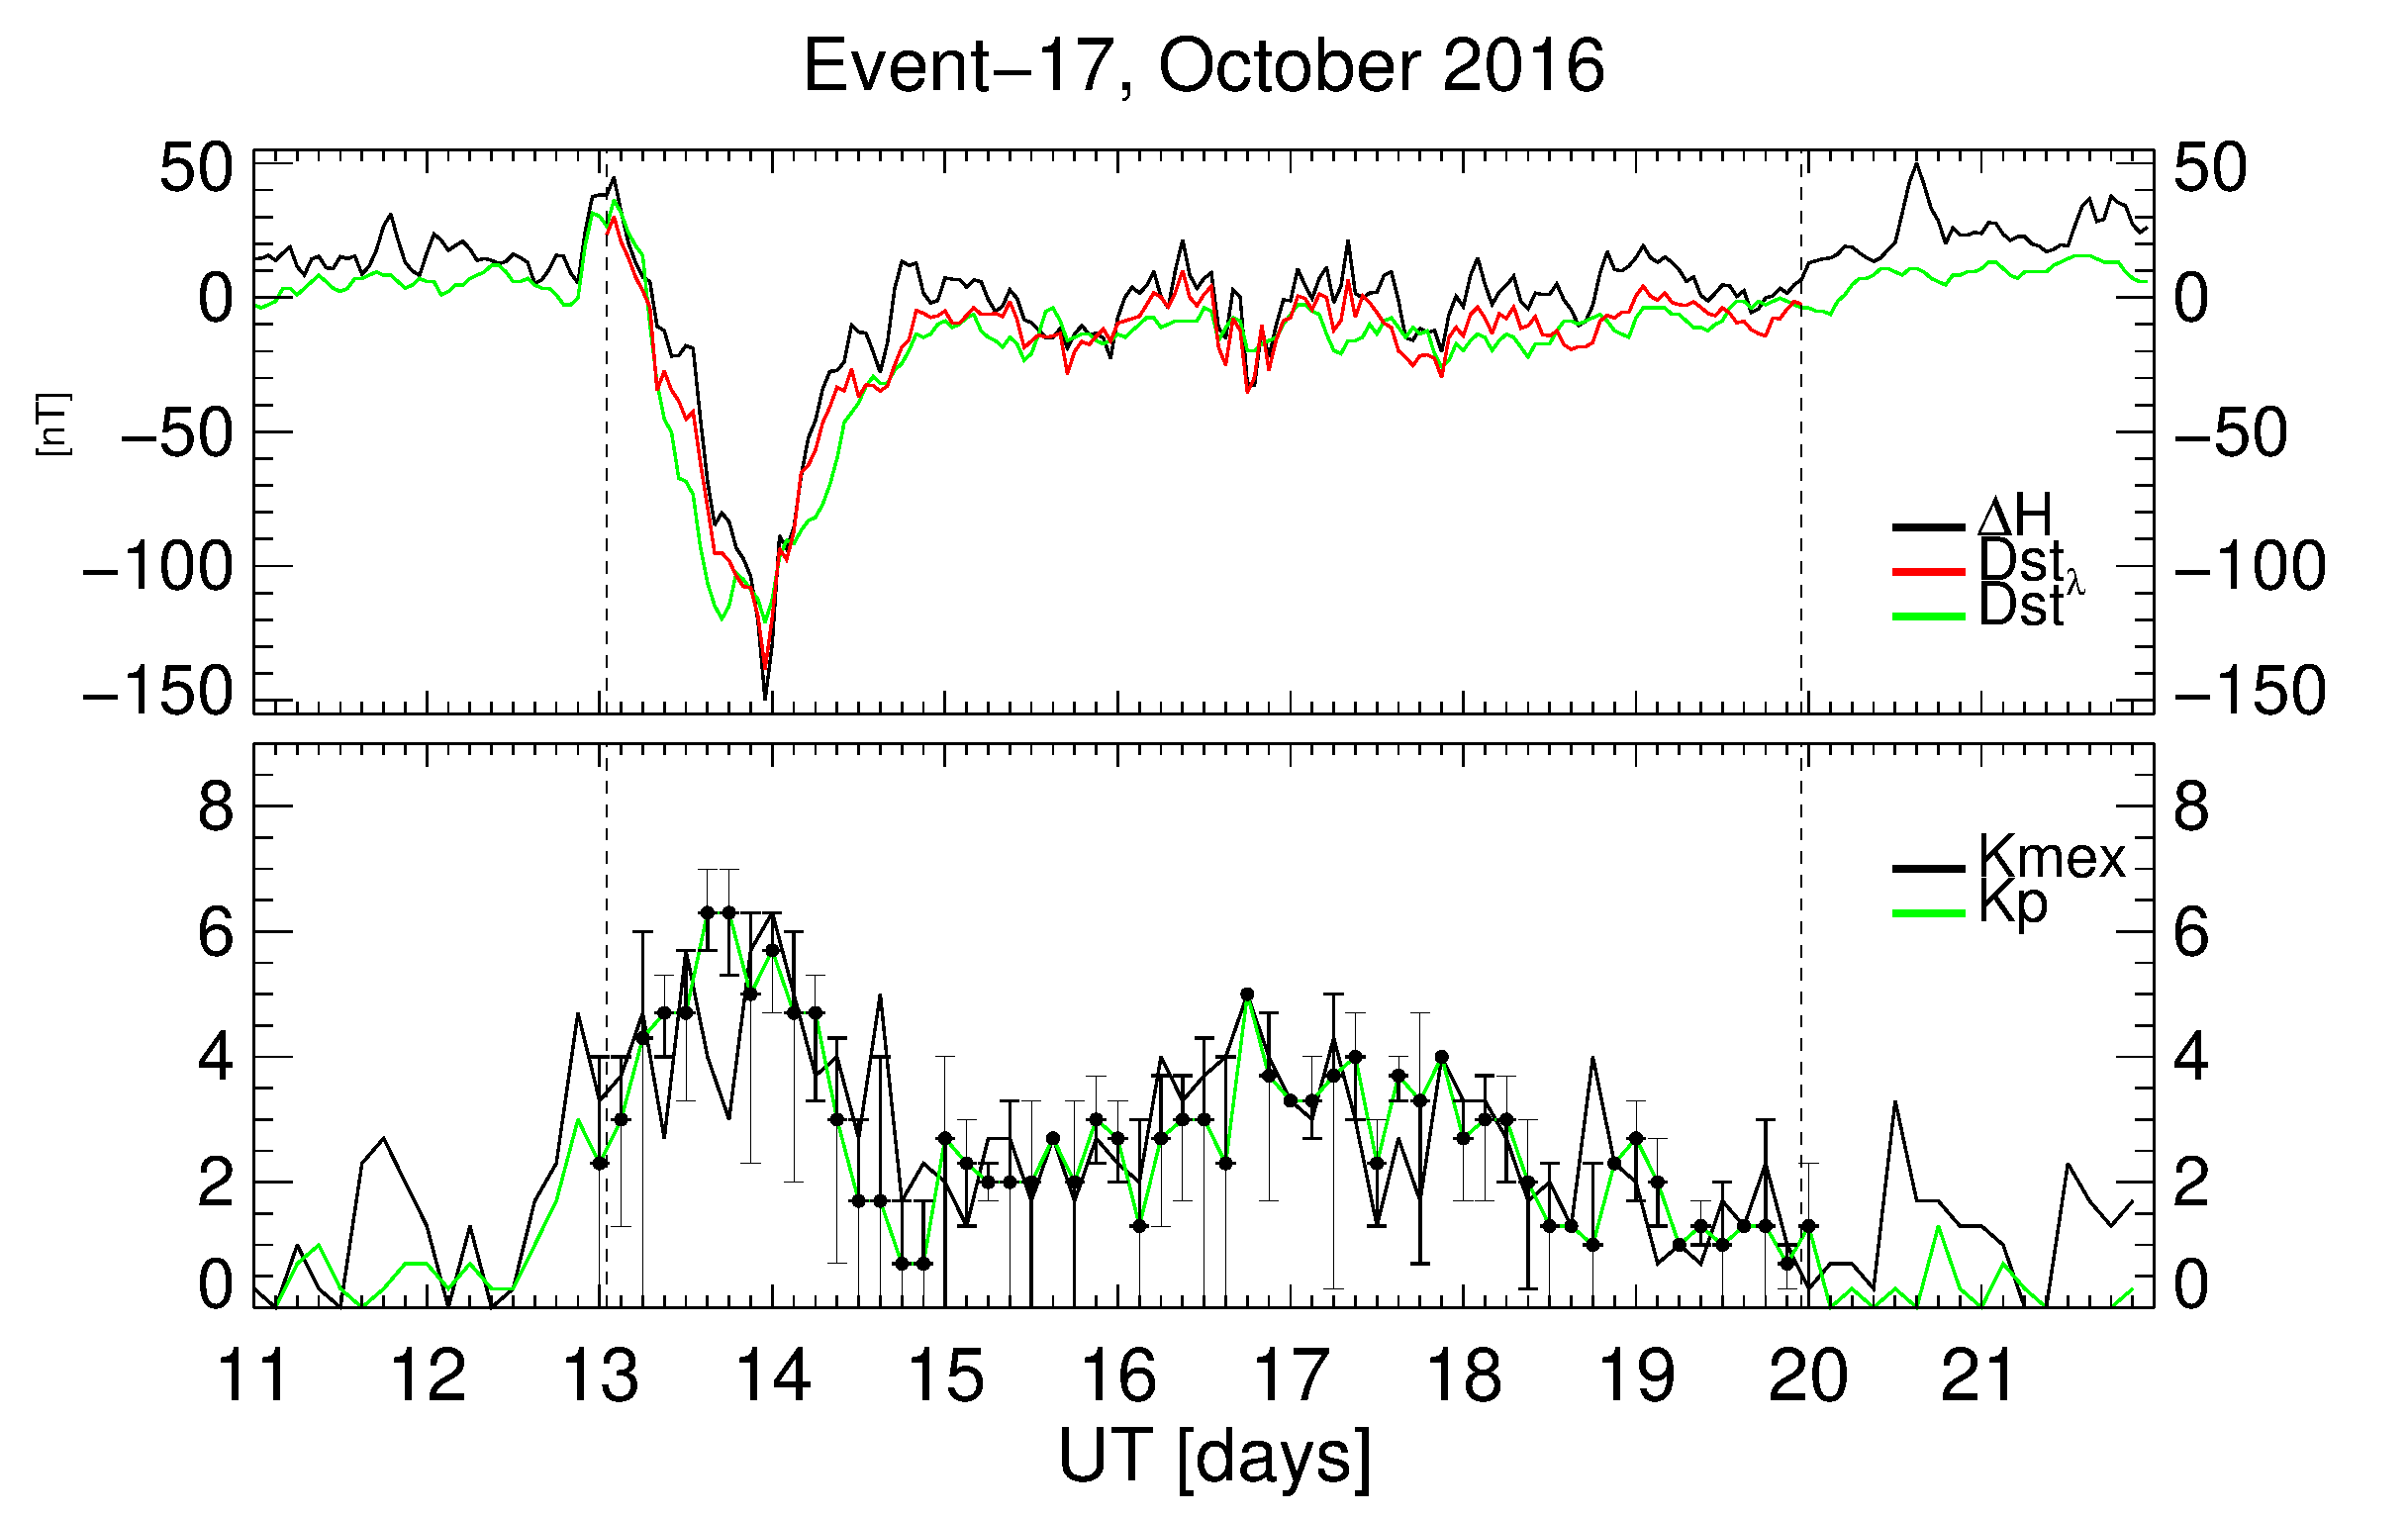
\includegraphics[width=6.0cm]{images/dH_approx/diono_valid_V4_2016-10-11.eps}     
       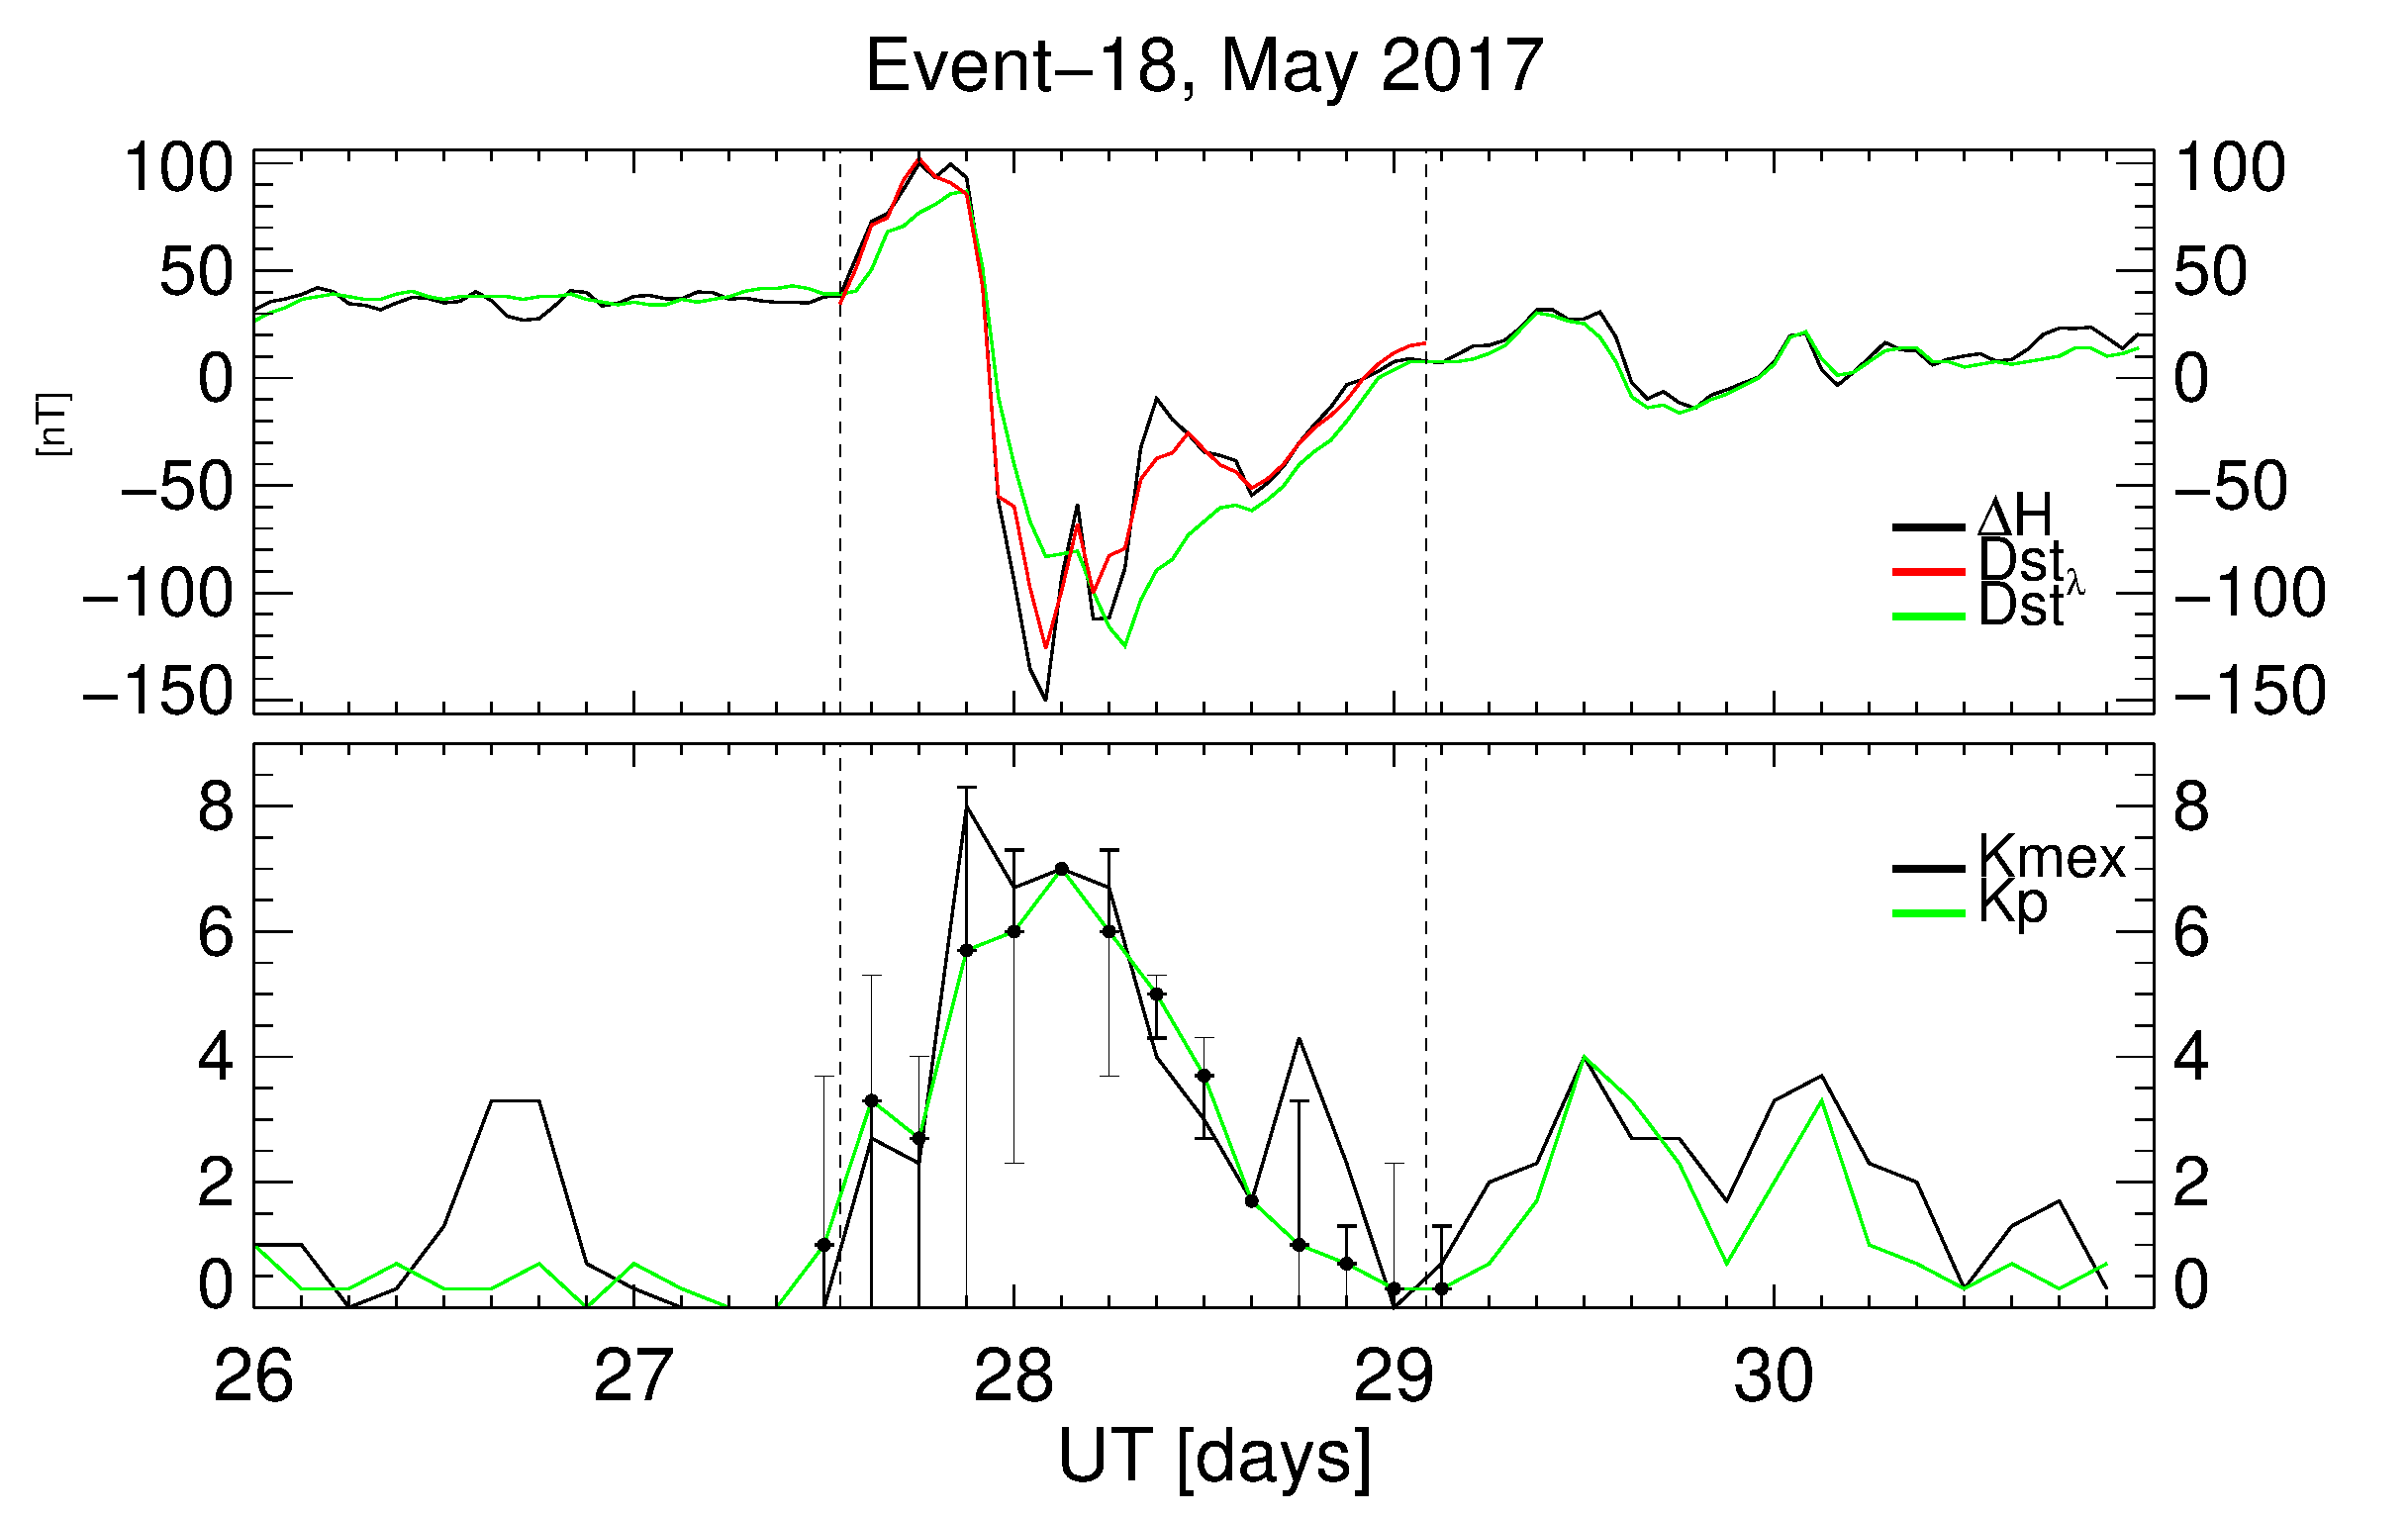
\includegraphics[width=6.0cm]{images/dH_approx/diono_valid_V4_2017-05-26.eps}

       \centerline{\Large \bf   
      \hspace{0.275\textwidth}  \color{black}{}
       \hspace{0.295\textwidth}  \color{black}{}
         \hfill}
       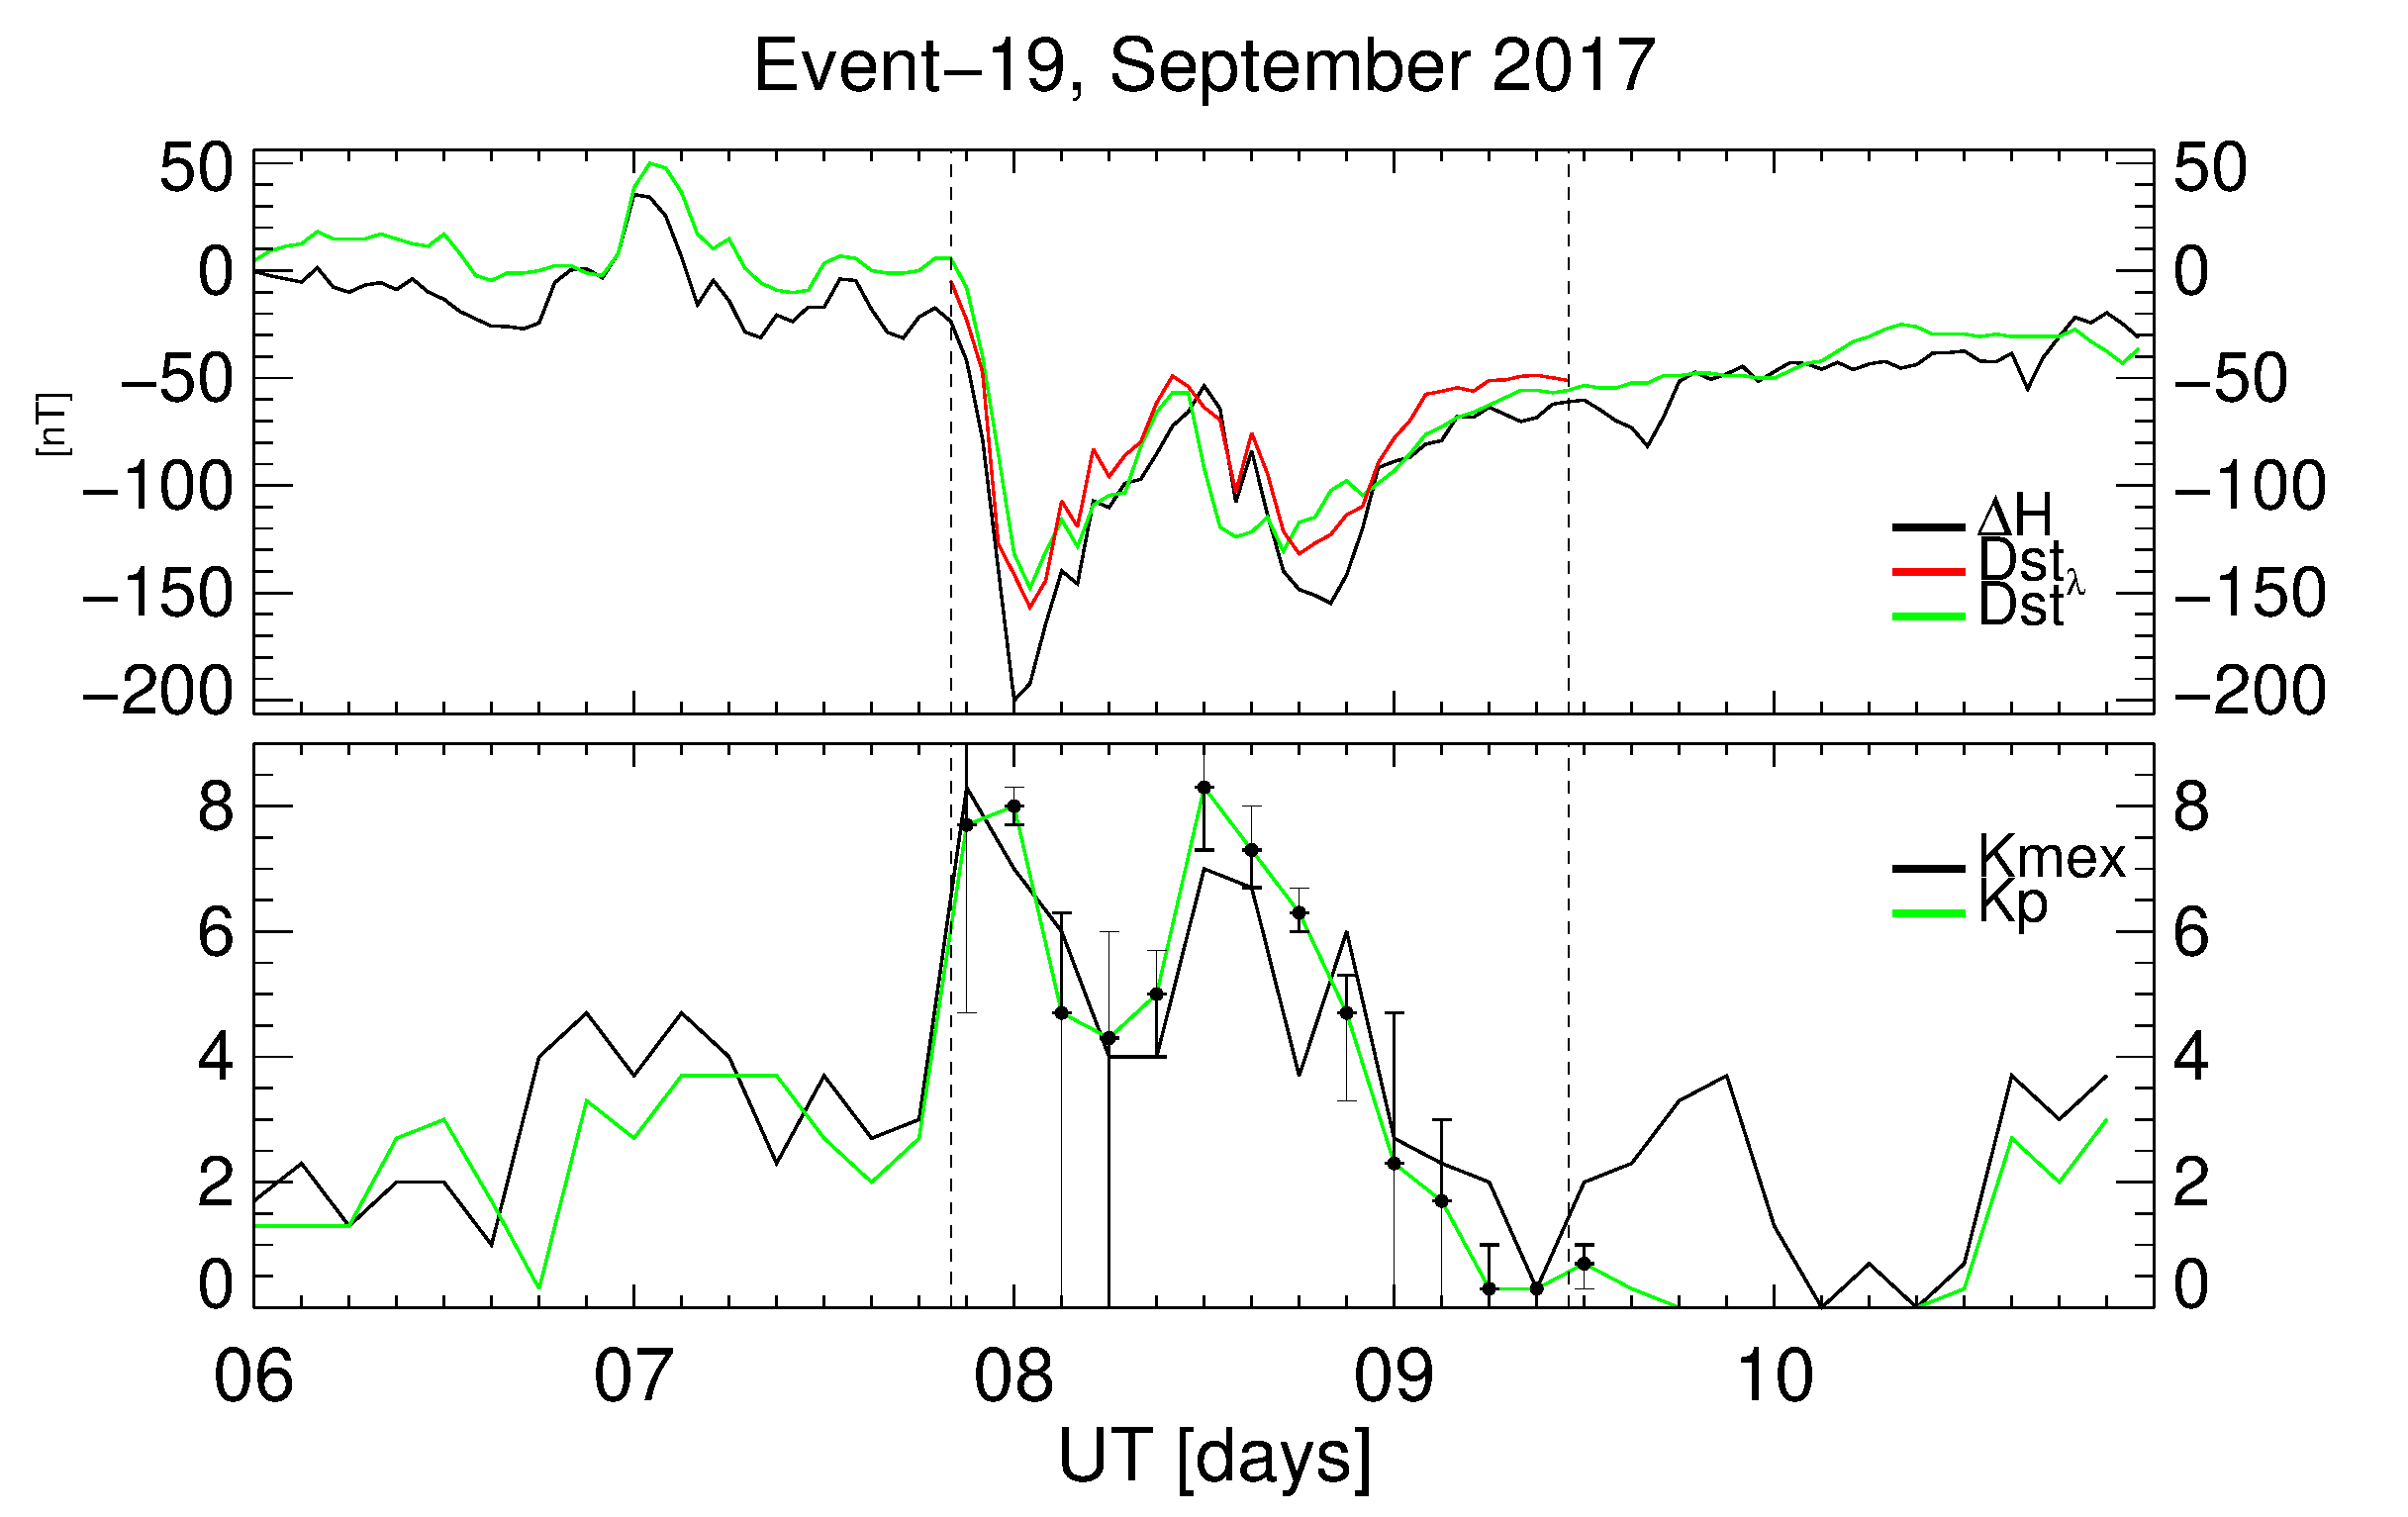
\includegraphics[width=6.0cm]{images/dH_approx/diono_valid_V4_2017-09-06.eps}     
       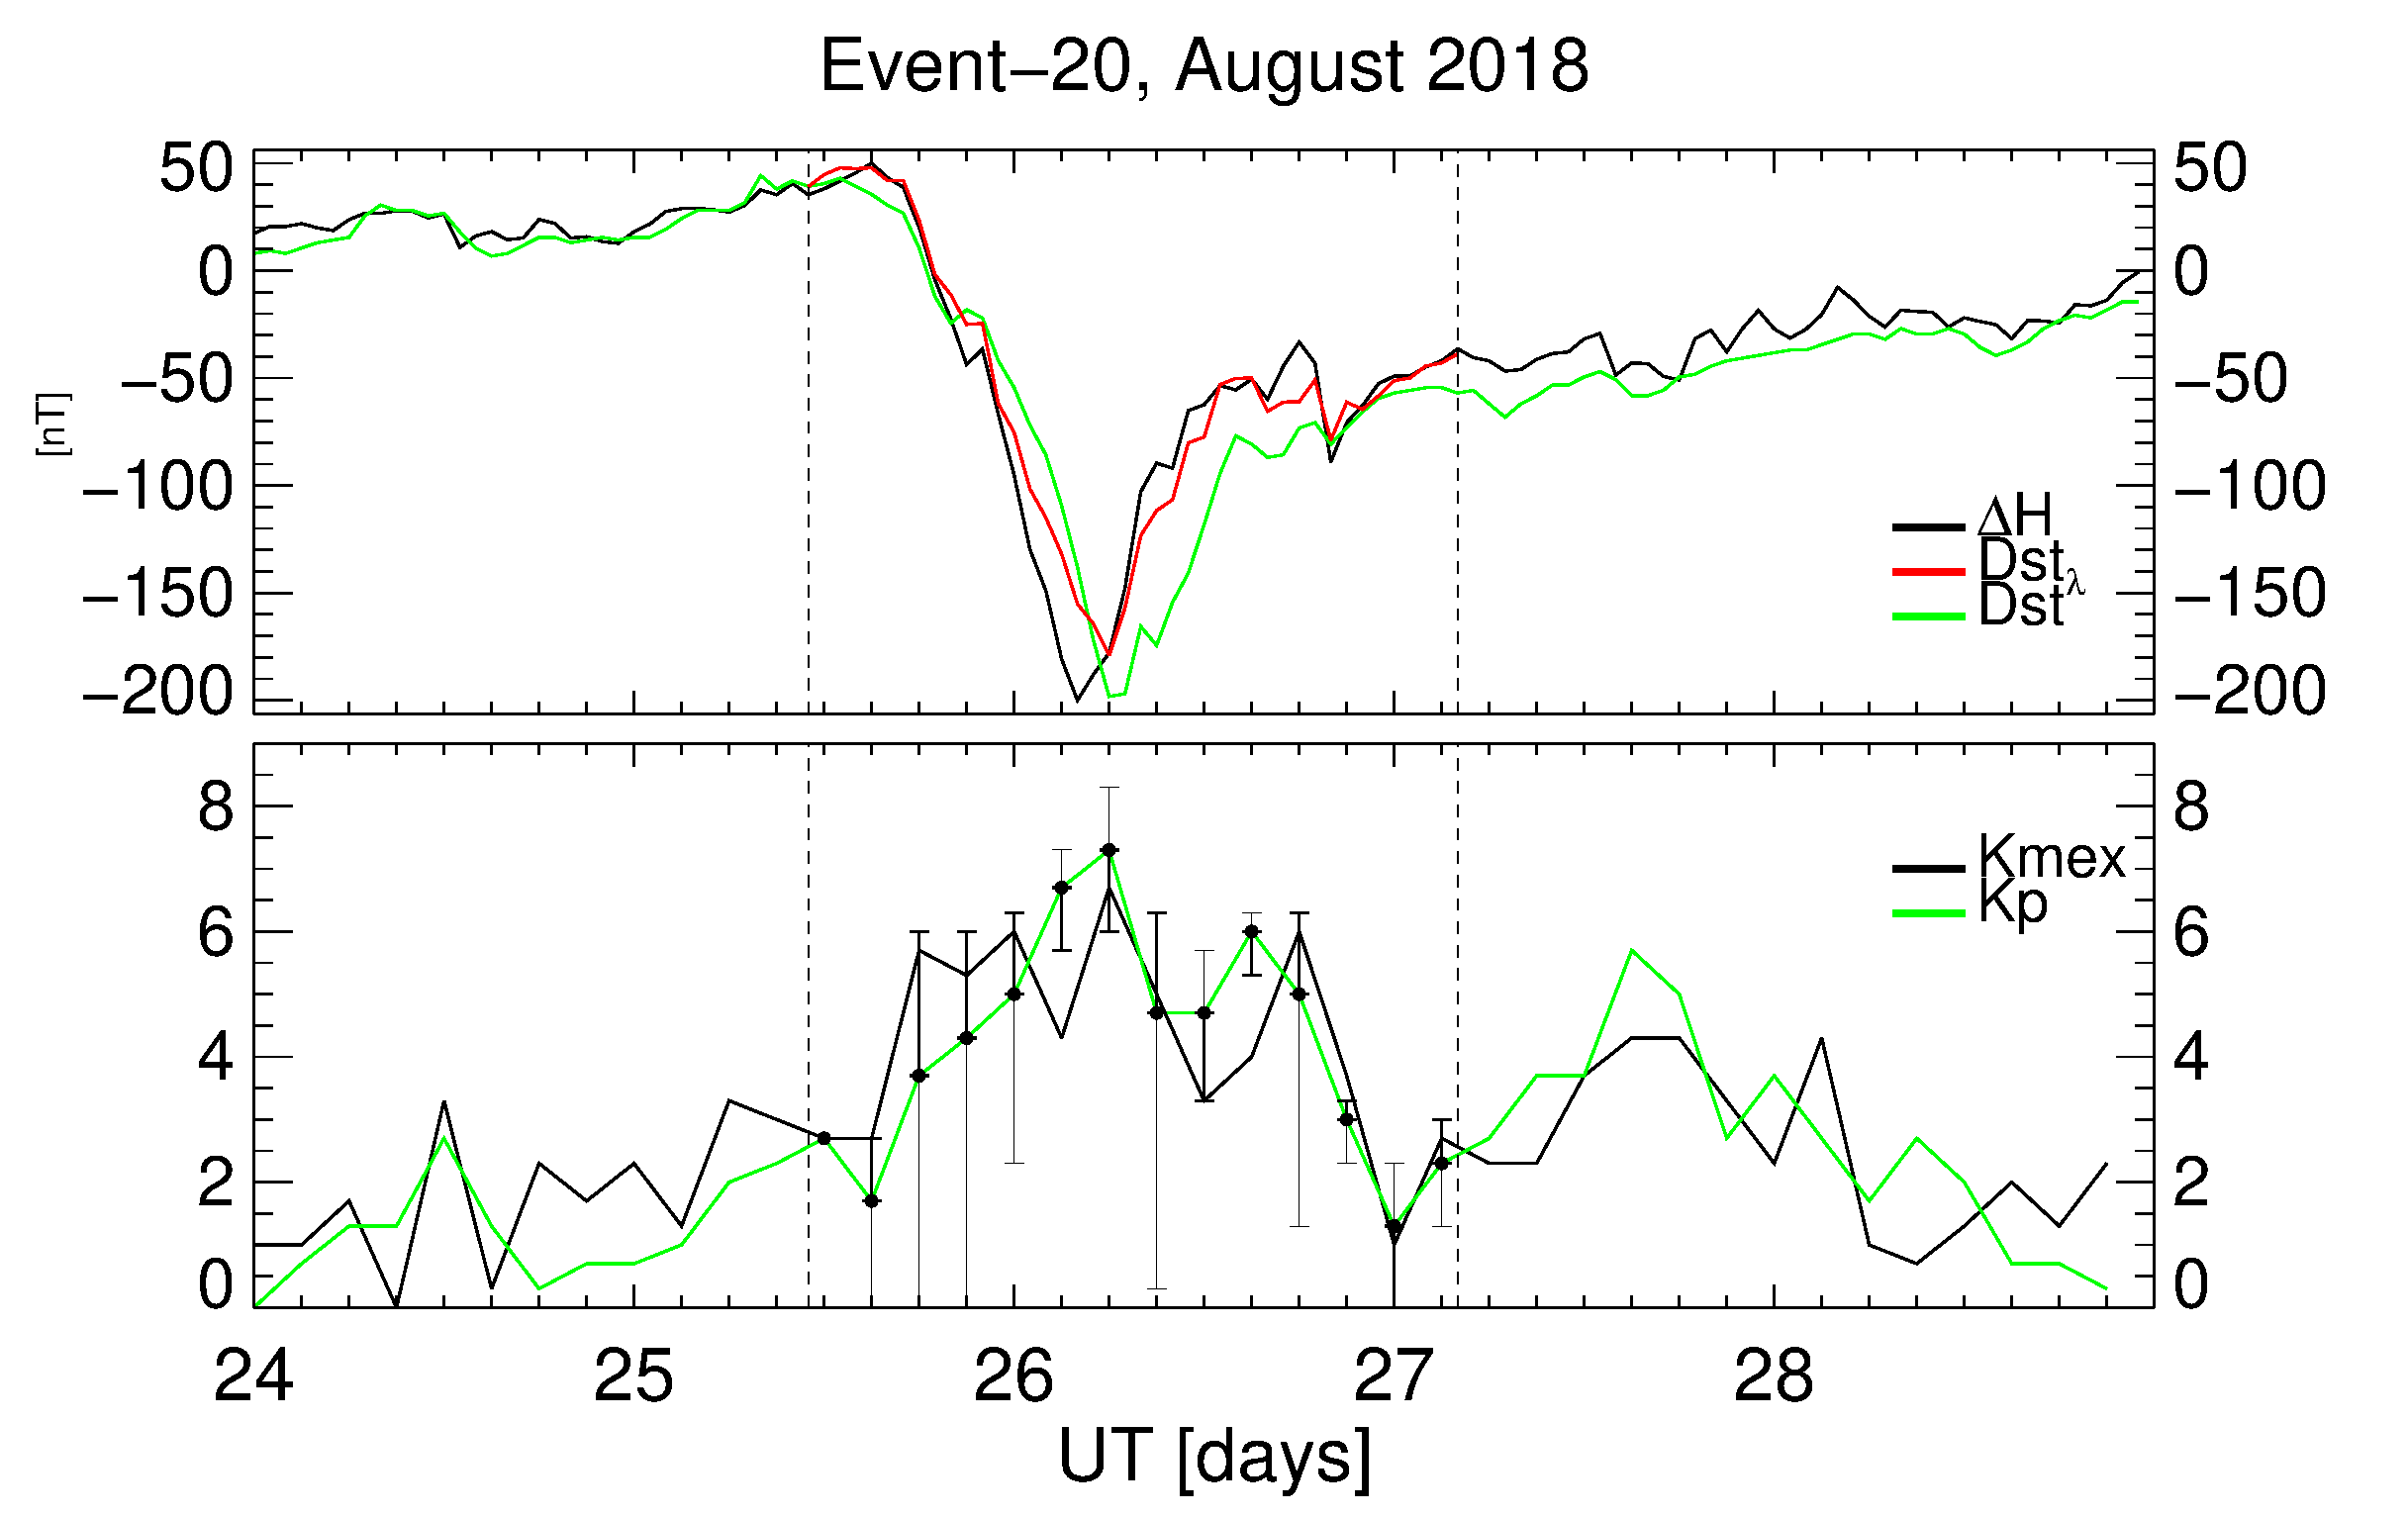
\includegraphics[width=6.0cm]{images/dH_approx/diono_valid_V4_2018-08-24.eps}
       
       \caption{Top: Approximation of $\Delta$H (red line). Bottom: Approximation of K local with a $\Delta$K affection range (error bars).}
    \label{fig:iono_valid3}
\end{figure*}



\end{document}

